% LaTeX Datei f�r Projektarbeiten etc. am MZH

% ------------------------------------------------------------------------------------------
% erlaubt das Anfangen des Draft-Modus und damit Ver�nderungen
% einzustellen
\newif\ifdraft
% Draft-Modus: Arbeitsversion, Bilder werden nur als Rahmen dargestellt
% Vorteil: schnelleres Kompilieren
%\drafttrue % <- daf�r hier die Kommentierung wegnehmen

%-------------------------------------------------------------------------------------------
% folgende Befehle sorgen daf�r, das f�r jede Schrift die richtigen Pakete installiert werden
\newcounter{schrift}
% Schrift ausw�hlen:
% 1 - mathptmx
% 2 - minionpro
% 3 - mathpazo
% 4 - times + computer modern
% 5 - computer modern
\setcounter{schrift}{4} % Hier die entsprechende Zahl setzen !

% ------------------------------------------------------------------------------------------
% ------------------------------------------------------------------------------------------
% Latex - Pr�ambel
% hier werden alle wichtigen Dokumenteinstellungen getroffen, normalerweise m�ssen
% keine �nderungen mehr durchgef�hrt werden.
% Pakete die das Schriftbild, den Satzspiegel oder die R�nder ver�ndern, d�rfen
% nicht hinzugef�gt werden, erst nach Abstimmung mit dem Betreuer.
% n�tzliche Pakete sind willkommen, bitte die Wiki entsprechend aktualisieren
% viele Pakete sind drin, die vielleicht nicht jeder braucht und das Kompilieren verl�ngern
% sollten diese das Layout nicht ver�ndern, k�nnen diese nat�rlich auskommentiert werden.
% ------------------------------------------------------------------------------------------

% ------------------------------------------------------------------------------------------
% Dokumentenklasse definieren:
\ifdraft
    \documentclass[draft, 
                   paper=a4,
                   BCOR5mm,
                   fontsize=12pt, 
                   DIV13, 
                   headsepline, 
                   numbers=noenddot, 
                   %bibtotoc,
                   bibliography = totoc,
                   %version=first,
                   %smallheadings,
                   headings = small,
                   oneside]{scrbook}
\else
    \documentclass[paper=
                   a4,
                   BCOR5mm,
                   fontsize=12pt, 
                   DIV13, 
                   headsepline, 
                   numbers=noenddot, 
                   %bibtotoc,
                   bibliography = totoc, 
                   %version=first,
                   %smallheadings,
                   headings = small,
                   headinclude=true,
                   footinclude=false,
                   fleqn, % formeln links b�ndig
                   oneside,
                   enabledeprecatedfontcommands]{scrbook}
\fi
% Standard-Koma-Dokument mit
%   Papierformat A4
%   Binderand 5 mm
%   Schrift 12-Punkt
%   Seitenlayout nach DIV, siehe scrguide.pdf text b/h rand oben/innen: 168,00 237,60 19,80 14,00 (ist raus)
%   Linie unter der Kopfzeile
%   Nummern ohne Punkt am Ende
%   Literaturverzeichnis im Inhaltsverzeichnis
%   �berschriften etwas kleiner als standard
%   weitere Informationen zum Koma-Skript: www.komascript.de

%---------------------------------------------------------------
% Basis-Pakete
%---------------------------------------------------------------
\usepackage{ifpdf}		%   Ueberprueft, ob LaTeX oder pdfLaTeX verwendet wird (nur ab MikTeX 2.5)
\usepackage[T1]{fontenc}        %   8-Bit-Fonts
\usepackage{textcomp,latexsym}  %   zusaetzliche Symbole
\usepackage[ansinew]{inputenc}   %   Quelltext ist Latin-1 (d.h. Windows-) kodiert
\usepackage[ngerman]{babel}            %   neue deutsche Rechtschreibung
\usepackage{scrtime}            %   fuer die aktuelle Zeit
%\usepackage{scrdate}            %   fuer das aktuelle Datum
%\usepackage{natbib}             %   Literaturverweise mit (Autor Jahr) nach DIN
%\bibpunct[; ]{[}{]}{,}{a}{}{;}  %   eckige Klammern statt runde bei Zitaten
%\usepackage[T1]{url}            %   Web-Addressen auch mit T1-Encoding
%\urlstyle{tt}                   %   und in tt-Font
%\usepackage[activate=normal]{pdfcprot} % dient dem optischen Randausgleich bei k�rzeren Zeichen wie '-', '.', ',', '!'

\usepackage{color}

\PassOptionsToPackage{x11names}{xcolor}
\usepackage{xcolor}


%---------------------------------------------------------------
% n�tzliche Zusatz-Pakete
%---------------------------------------------------------------
%\usepackage{makeidx}            %   Index (wenn gewuenscht)

\usepackage{setspace}           %   Zeilenabstand setzen. Befehl:
                                %   \begin{spacing{Wert}
                                %   Text
                                %   \end{spacing}
%\usepackage{placeins}           %   das Positionieren von float-Umgebungen bestimmen:
                                %   der Befehl \floatbarrier sorgt daf�r, dass alle vorher eingegebenen
                                %   float-Umgebungen VOR diesem Befehl eingef�gt werden.
                                
%\usepackage{subfig}          %   Bilder gruppieren, mehrere Bilder in einer Umgebung einf�gen
                                %   Bsp.:
                                %   \begin{figure}
                                %   \centering
                                %    \subfloat[Text a]
                                %    {\includegraphics{bild a}}
                                %    \subfloat[text b]
                                %    {\includegraphics{bild b}}
                                %    \caption{Untertitel}
                                %    \label{fig.Beziechnung_subfigure} <- am besten mit fig. dann kann mit \bild{Bezeichnung_figure} referenziert werden
                                %   \end{figure}                                

%\usepackage{textcomp}           %   fuer Trademark und Copyright Zeichen
                                %   z.B \texttrademark, \textregistered, \texteuro etc.

\usepackage{tabularx}           %   erweiterte Funktionen f�r Tabellen

\usepackage{longtable}          %   Longtable-Package f�r Tabellen die l�nger als eine DIN-A4-Seite sind

\usepackage{colortbl}						%		farbige Tabellenzeilen

\usepackage{nicefrac}           %   Schr�ge Bruchstriche \nicefrac{Nenner}{Z�hler}

%\usepackage{numprint}           %   Zahlen mit Einheiten n�her an der Zahl/kein Umbruch und 1 000er Format \numprint[Einheit]{Zahl}

%\usepackage{mathcomp}           %   f�r \tcdegree (� Gradzeichen bei numprint) \numprint[\tcdegree]{180} f�r 180�

%\usepackage{hhline}             %   hhline-Package
                                %   Fuer komplexe Linienzuege in Tabellen \hhline{}
                                %   = Spalte mit doppelter Linie      | vertikale Linie die horizontale schneidet
                                %   - Spalte mit einfacher Linie      : vertikale Linie die von horizantaler unterbrochen ist
                                %   ~ Spalte ohne Linie               # doppelte horiz. geschnitten mit doppelter vert. Linie
                                %   t oberer Teil ->                  b unterer Teil einer doppelten Linie

%\usepackage[active]{srcltx}     %   bei verwendung v. \includeonly spring winedt jetzt bei fehlern an die richtige stelle

\usepackage{flafter}            %   Ein float-Objekt immer erst NACH seiner Definition platzieren

\usepackage{ifthen}             %   definiert \ifthenelse{}{}{}

%\usepackage{path}               %   dateinamen und pfade darstellen

%\usepackage{pdfsync}						%   Synchronisation mit SumatraPDF <<-- geht auch ohne

\usepackage{booktabs}

%% Eigene Pakete

\usepackage{scrhack} % L�scht Warnungen von Packages wie hyperref, listings
\usepackage[ locale = DE,            % deutsch
            load-configurations=abbreviations, % zus�tzliche Einheiten siehe manual
            per-mode=symbol,%-or-fraction,
            separate-uncertainty% 
            ]
            {siunitx}								% SI-Einheiten  

            
\usepackage{multirow}               % zwei Zeilen kombinieren (wie multicolumn)
\usepackage[babel]{microtype}       % schickeres Schriftbild -> aber l�ngeres Kompilieren

\usepackage{blindtext}							% sinnlosen text einbauen
\usepackage{subfigure}

\usepackage{newunicodechar}
%\newunicodechar{ }{~}

%\DeclareUnicodeCharacter{00A0}{~}


%%

%---------------------------------------------------------------
% Grafik-Paket f�r eps bzw. pdf
%---------------------------------------------------------------
% �berpr�ft ob Latex oder PDFLatex ausgef�hrt wird, dementsprechend werden pdf/jpg oder eps Bilder eingef�gt
% sollen dvi oder pdf Dokumente erstellt werden m�ssen alle Bilder in beiden Formaten vorliegen
% hierf�r gibt es Tools wie epstopdf oder jpgtoeps
 \ifdraft
    \usepackage[draft]{graphicx}
\else
    \ifpdf
        \usepackage{graphicx}
        \usepackage{pgfplots} % pgfplots zum plotten in LaTeX
    \else
        \usepackage[final]{graphicx}
    \fi
\fi
% von wo sollen die Grafiken kommen?
\graphicspath{{./fotos/}{./skizzen/}{./zeichnungen/}{./plots/}{./bilder/}}

%Einstellungen f�r pgfplots
\pgfplotsset{compat=1.3,
	%enlargelimits=auto,
	tick label style={font=\small,/pgf/number format/use comma}, %Komma nutzen in allen Axen
	%axis x line=center, %alle x-Achsen center
	%axis y line=center, %alle y-achsen center
	%every axis x label/.style={at={(current axis.right of origin)},anchor=west}, % achsenbeschriftung bei allen x-achsen rechts
	%every axis y label/.style={at={(current axis.above origin)},anchor=south},   % achsenbeschriftung bei allen y-achsen oben
	%every x tick scale label/.style={at={(current axis.right of origin)},anchor=north,yshift=-0.5em}, %positionierung des scale faktors ge�ndert
	every axis legend/.append style={at={(1.0,0.5)},anchor=west,nodes=right,font=\small}, % Legende �ber der Grafik, schriftgr��e small
	label style={font=\small}, % label schriftgr��e small
	ticklabel style={% gilt f�r x und y
		/pgf/number format/.cd,
		use comma,% Komma als Dezimaltrenner
		1000 sep = {}% keine Tausendertrennung 
	}
}
\newlength\tikzwidth
\setlength{\tikzwidth}{0.7\textwidth}
\definecolor{mycolor1}{rgb}{0,0.5,0}

\ifpdf
 \ifdraft
    \usepackage[draft]{pdfpages}%   externe PDF Seiten einbinden nur bei PDF-Latex m�glich
    \else
    \usepackage[final]{pdfpages}%   externe PDF Seiten einbinden nur bei PDF-Latex m�glich
 \fi                            %   Befehl: \includepdf{PDF-Datei} soll die Datei im Querformat angezeigt werden
    \else
\fi                             %   \includepdf[landscape=true]{PDF-Datei}

%---------------------------------------------------------------
% Debug-Ausgabe der Labels und References
%---------------------------------------------------------------
\ifdraft
  \usepackage{showkeys} % Label werden im Draft Modus im Text angezeigt
\fi

%---------------------------------------------------------------
% Abweichende PostScript-Schriftarten
% werden in der main Datei ausgew�hlt, hier nichts �ndern
%---------------------------------------------------------------
\ifthenelse{\equal{ 1 }{ \value{schrift} }}
    {
    \usepackage{mathptmx}          %   Times als Hauptschriftart, keine mathematische Fettschrift
    \usepackage{amssymb}
    \usepackage{amsbsy}
    \usepackage{amsmath}
    \usepackage{amsfonts}
    \usepackage{amstext}
    \renewcommand{\boldsymbol}[1]{\mathbf{#1}} % nur bei mathptmx !
                                               % damit boldsymbol wenigstens fette aufrechte Buchstaben macht
    }{}
\ifthenelse{\equal{ 2 }{ \value{schrift} }}
    {
    \usepackage[lf, minionint]{MinionPro} %   OpenType von Adobe, mathematische Fettschrift vorhanden, Schrift ist
                                %   ist im Standard-LaTeX nicht installiert.
                                %   Ist ein wenig Aufwand das Ganze zu installieren, Matthias Dagen fragen
    }{}
\ifthenelse{\equal{ 3 }{ \value{schrift} }}
    {
    \usepackage{mathpazo}          %   nette Buchschrift aber sehr gross, mathematische Fettschrift vorhanden
    \usepackage{amssymb}
    \usepackage{amsbsy}
    \usepackage{amsmath}
    \usepackage{amsfonts}
    \usepackage{amstext}
    }{}
\ifthenelse{\equal{ 4 }{ \value{schrift} }}
    {
    \usepackage{times}
    \usepackage{amssymb}
    \usepackage{amsbsy}
    \usepackage{amsmath}
    \usepackage{amsfonts}
    \usepackage{amstext}
    }{}
\ifthenelse{\equal{ 5 }{ \value{schrift} }}
    {
    \usepackage{amssymb}
    \usepackage{amsbsy}
    \usepackage{amsmath}
    \usepackage{amsfonts}
    \usepackage{amstext}
    \usepackage{lmodern}
    }{}
\usepackage[scaled=.92]{helvet} %   11pt Helvetica f�r �berschriften etc. etwas kleiner da, Helvetica an sich gr��er ist
%\usepackage{courier}            %   Courier bei \texttt
%\usepackage{upgreek}            %   Aufrechte griechische Buchstaben

% ------------------------------------------------------------------------------------------
% Bild- und Tabellentitel FETT
% ------------------------------------------------------------------------------------------
%\def\figurename{\bfseries Bild}
%\def\tablename{\bfseries Tabelle}

%%Andere Beschreibung von figure
\addto\captionsngerman{
	\renewcommand{\figurename}{\bfseries Bild}%%Andere Beschreibung von figure
	\renewcommand{\listfigurename}{Bildverzeichnis}
	\renewcommand{\tablename}{\bfseries Tabelle}
}

%---------------------------------------------------------------
% Quelltexte formatieren
%---------------------------------------------------------------
\usepackage{listings}


%\lstloadlanguages{
		%C,
		%C++,
		%XML
%}

\lstset{
		language=XML,
		basicstyle=\footnotesize\ttfamily, % Standardschrift
		numbers=left,               % Ort der Zeilennummern
		numberstyle=\tiny,          % Stil der Zeilennummern
		numbersep=5pt,              % Abstand der Nummern zum Text
		tabsize=2,                  % Groesse von Tabs
		extendedchars=true,         %
		breaklines=true,            % Zeilen werden Umgebrochen        
		keywordstyle=\color{Red2},
		frame= b,         
		stringstyle=\color{Purple2}\ttfamily, % Farbe der String
		showspaces=false,           % Leerzeichen anzeigen ?
		showtabs=false,             % Tabs anzeigen ?
		xleftmargin=17.5pt,
		framexleftmargin=17pt,
		framexrightmargin=5pt,
		framexbottommargin=4pt,
		linewidth= \dimexpr\textwidth-2\fboxsep-2\fboxrule,
		comment=[l]{\#},
		morecomment=[s]{<!--}{-->},
		commentstyle=\color{Green4},
		%backgroundcolor=\color{grey},
		showstringspaces=false,      % Leerzeichen in Strings anzeigen ?        
		morekeywords={__global__, name, pkg, args, type, from, to, textfile, respawn, value, output, radius, ixx, ixy, ixz, iyy, iyz, xyz, rpy, reference},  % CUDA specific keywords
		aboveskip = 18pt, 
		belowskip = 18pt
}

\usepackage{caption}
\DeclareCaptionFont{white}{\color{white}}
\DeclareCaptionFormat{listing}{\colorbox{darkgray}{\parbox{\dimexpr\textwidth-2\fboxsep-2\fboxrule}{\hspace{15pt}#1#2#3}}}
\captionsetup[lstlisting]{format=listing,labelfont=white,textfont=white, singlelinecheck=false, margin=0pt, font={bf,footnotesize}}

%---------------------------------------------------------------
% ein paar L�ngen einstellen
%---------------------------------------------------------------
%\setlength{\parskip}{1ex plus0.5ex minus0.2ex} % Absatzabstand etwas gr��er
\setlength{\itemsep}{0ex plus0.2ex}            % Abstand zweier Listenelemente kleiner
\setlength{\parindent}{0ex}                     % kein Absatzeinzug
\setlength{\belowcaptionskip}{0.4cm}            % Abstand caption - Tabelle gr��er
\setlength{\abovecaptionskip}{0.4cm}            % Abstand caption - Tabelle gr��er

%---------------------------------------------------------------
% Kopf- und Fusszeilen
%---------------------------------------------------------------
\usepackage[plainheadsepline,  % linie zw. kopf und text auch bei seitenstil "plain"
           %headexclude,       % kopfzeile geh�rt nicht zum textk�rper
           %footexclude        % fusszeile geh�rt nicht zum textk�rper
          ]       
           {scrpage2}
\pagestyle{scrheadings}
\clearscrheadfoot              % voreinstellungen loeschen
\ihead{\normalfont\headmark}   % kolumnentitel innen
\ohead[\pagemark]{\pagemark}   % seitenzahl aussen

%---------------------------------------------------------------
% Nummerierungs-Tiefe des Inhaltsverzeichnis und der Abschnitte einstellen
%---------------------------------------------------------------
\setcounter{secnumdepth}{2} \setcounter{tocdepth}{2}

%---------------------------------------------------------------
% Abk�rzungsverzeichnis
%---------------------------------------------------------------
% mit dem Befehl \nomenclature[l/g/a]{Abk�rzung}{Bezeichnung} kann direkt im Code die Abk�rzung eingef�gt werden
% das Paket sortiert diese und f�gt sie mit dem Befehl \printnomenclature ein
% l, g, oder a steht dabei f�r die Gruppierung Lateinische bzw. Griechische Buchstaben, Abk�rzungen
% Nach Einf�gen neuer Abk�rzungen muss folgender Befehl in der Eingabeaufforderung im Tex-Verzeichnis eingegeben werden:
% -> vorher einmal kompilieren
% -> makeindex main.nlo -s nomencl.ist -o main.nls
% -> nochmal kompilieren
%\makeindex
\usepackage{nomencl}
% \let\abbrev\nomenclature
\renewcommand{\nomname}{Symbolverzeichnis}
\setlength{\nomlabelwidth}{.2\hsize}
\renewcommand{\nomlabel}[1]{#1 \hfill}
\setlength{\nomitemsep}{-\parsep}

\renewcommand{\nomgroup}[1]{%
	\ifthenelse{\equal{#1}{A}}{\item[\textbf{Doppelpendel}]}
	{%	
		\vspace{4.5cm}
		\ifthenelse{\equal{#1}{B}}{\item[\textbf{Zustandsregelung}]}
		{%
%			\vspace{0.5cm}
			\vspace{-2cm}
			\ifthenelse{\equal{#1}{C}}{\item[\textbf{Nichtlineare Zustandsbeobachtung}]}
			{
				\vspace{4.2cm}
				\ifthenelse{\equal{#1}{D}}{\item[\textbf{Beobachtervalidierung}]}{}
			}
		}
	}
}

\makenomenclature

%---------------------------------------------------------------
% Hyperlinks f�r pdfTeX
%---------------------------------------------------------------
\ifpdf
    % hier stehen befehle, die nur f�r pdftex gelten
    \usepackage[pdfpagelabels,  % logische (z.b. auch roemische) seitenzahlen
                bookmarks,       % Bookmarks f�r die einzelnen Abschnitte
                pdftex
                ]{hyperref}
    \hypersetup{
    %   colorlinks,  % Links mit farbigem Text
        pdfborder   = 0 0 0,
        plainpages  = false,
        bookmarksnumbered = true,
    %   bookmarksopen
    }
\else
    % hier stehen befehle, die nur f�r latex gelten
    \usepackage{hyperref} % hier ohne colorlinks und pdf-krams
\fi

%extra inhaltsverzeichnisse m�glich
\usepackage[nohints]{minitoc}     
\renewcommand{\mtctitle}{Anhangsverzeichnis} 				% Name �ndern            
\renewcommand{\mtifont}{\large\bfseries\sffamily}			% Titel font �ndern
\renewcommand{\mtcSfont}{\rm}								% Section eintr�ge normal
\mtcsetrules{minitoc}{off}									% Linien ausmachen

%---------------------------------------------------------------
% SVGs einf�gen
%---------------------------------------------------------------
%% SVG to TeX
% from InkscapePDFLaTeX.pdf
% by Johan Engelen, 2010
% Information: 
% http://tug.ctan.org/tex-archive/info/svg-inkscape
% -shell-escape muss im Ausgabeprofil stehen
% inkscape.exe muss im Path-Folder sein

% Funktion zum ueberpruefen auf Aenderung
\newcommand{\executeiffilenewer}[3]{%
                \ifnum\pdfstrcmp{\pdffilemoddate{#1}}%
                {\pdffilemoddate{#2}}>0%
                {\immediate\write18{#3}}\fi%
}
% Wenn Aenderung dann TeX-Export ausfuehren und einbinden
%\newcommand{\includesvg}[1]{%
                %\executeiffilenewer{#1.svg}{#1.pdf}%
                %{inkscape -z -C --file=#1.svg %
                %--export-pdf=#1.pdf --export-latex}%
                %\input{#1.pdf_tex}%
%}

%% Include svg mit Text aus textext plugin
% text wird im svg mit textext hinzugef�gt.
% falls �nderungen im .svg gefunden werden, wird das Bild 
% neu exportiert und eingef�gt.
% \includesvg{ordner/file} /ohne endung
\newcommand{\includesvg}[4][]{
			\executeiffilenewer{#3.svg}{#3.pdf}
			{inkscape -z -D --file=#3.svg
			--export-pdf=#3.pdf}
			\begin{figure}[#2]
				\centering
				\includegraphics[#1]{#3}
				\caption{#4} \label{fig.#3}
				\vspace*{-3mm}
			\end{figure}
}

\newcommand{\includesinglesvg}[2][]{
			\executeiffilenewer{#2.svg}{#2.pdf}
			{inkscape -z -D --file=#2.svg
			--export-pdf=#2.pdf}
			\includegraphics[#1]{#2}
}

\usepackage[right]{eurosym}

                           % Pr�ambel zur Dokumentenformatierung einf�gen
                                            % braucht nicht zu ver�ndert werden, stehen aber n�tzliche
                                            % Hinweise drin

%---------------------------------------------------------------
% Trennmuster fuer Ausnahmef�lle
%---------------------------------------------------------------
\hyphenation{} % z.B. \hypenation{Trenn-text}
\hyphenation{Kraft-ein-wirk-ung}
\hyphenation{ein-ge-spannt}
\hyphenation{Coch-lea-im-plan-ta-te}
\hyphenation{Deh-nungs-mess-streifen}

%---------------------------------------------------------------
% Dokumentenanfang:
%---------------------------------------------------------------
% Einstellungen f�r PDF-Latex:
% Hier Titel etc. eintragen, dann wird es in den Dokumenteneigenschaften vom PDF richtig angezeigt
\ifpdf
    \hypersetup{
    %   colorlinks,  % Links mit farbigem Text
        pdftitle    = {Nichtlineare Zustandsbeobachtung mit bildbasierter Validierung am inversen Doppelpendel},
        pdfsubject  = {Studienarbeit},
        pdfauthor   = {Andreas Serov},
        pdfkeywords = {Zustandsbeobachtung, Doppelpendel}
        }
\else
\fi

\usepackage{caption}
\usepackage{tikz}							% package f�r blockschaltbilder in latex
\usetikzlibrary{arrows, decorations.markings, positioning,automata, positioning,arrows.meta,shapes.multipart}
\usepackage{pgfplots}
% for double arrows a la chef
% adapt line thickness and line width, if needed
\tikzstyle{vecArrow} = [semithick, decoration={markings,mark=at position
	1 with {\arrow[semithick]{open triangle 60}}},
double distance=1.4pt, shorten >= 5.5pt,
preaction = {decorate},
postaction = {draw,line width=1pt, white,shorten >= 4.5pt}]
\tikzstyle{innerWhite} = [semithick, white,line width=1pt, shorten >= 4.5pt]

\NewDocumentCommand{\angsi}{omom}{%			% f�r �/s
	\ang[#1]{#2}\si[#3]{#4}%
}

\usepackage{setspace}
\usepackage{afterpage}						% leere seite
\newcommand\blankpage{%
	\null
	\thispagestyle{empty}%
	\addtocounter{page}{-1}%
	\newpage}		
\usepackage{algorithmicx}					% f�r algorithmen
\usepackage{algpseudocode}					% f�r algorithmen
\usepackage{algorithm}						% f�r algorithmen
\usepackage{tabu}							% f�r dicke linien in tabellen
\usepackage{bm}								% bold math \bm{math expression}
\usepackage{mathtools}						% f�r *Matrizen zum Ausrichten der Eintr�ge
\usepackage{dsfont}							% $ x \in mathds{R} $
%\usepackage[utf8]{inputenc}				% umlaute
%\usepackage[ansinew]{inputenc}				% umlaute
\usepackage{befehle}                        % eigene Befehle wie:
                                            % \zB\,
                                            % \abbildung{Position h,b,t,p}{Dateiname ohne Endung}{Caption}
                                            % \bild{Dateiname}, referenziert gem�� ...Bild x.xx...
                                            % einfach mal nachschauen was so drin ist und eigene Befehle f�r
                                            % wiederholende Sachen definieren

%\includeonly{ergebnisse}                   % wenn nur ein Kapitel kompilliert werden soll
                                            % geht schneller wenn man nur das Layout des Kapitels sehen will

%\entwurf                                   % Entwurfsdatum auf jede Seite setzen,
                                            % nicht vergessen beim Druck rauszunehmen
%\setlength\overfullrule{5pt}                % Overfull boxes werden angezeigt
%\setlength\underfullrule{5pt} 

% Seitenspiegel neu berechnen
\typearea[current]{last}

%\typearea{last}
\begin{document}                            % Dokumentenanfang
\dominitoc
\begin{spacing}{1.15}                       % Zeilenabstand auf 1,15 fach stellen, ist nicht so eng aber
                                            % auch nicht so eine Seitenschinderei wie 1,5-fach
    \frontmatter                            % mit kleinen r�mischen Seitenzahlen beginnen f�r class scrbook
    %\pagenumbering{roman}                  % das gleiche f�crartcl
    \setcounter{page}{0}
    \pdfbookmark[0]{Titel}{tit}             % damit der Titel auch im Acrobat angezeigt wird
		\begin{titlepage}
\begin{spacing}{2}

\begin{flushright} %rechtsb�ndig (Anfang)
	\vspace*{-20mm}
	\includegraphics[width=\textwidth]{skizzen/CoverLogos}
	%\includegraphics[width=\textwidth]{skizzen/CoverLogos_MZH}
\end{flushright} %rechtsb�ndig (Anfang)

% der Titel der Arbeit:
\vspace{38mm} {\centering {{\LARGE{Test Kartierung und Selbstlokalisierung f�r eine
									 omnidirektionale mobile Roboterplattform
									 in unbekanntem Terrain}}}

\vfill
% hier kommt ne h�bsche Grafik hin:
%\includegraphics[width = 80mm]{youBot}


\vfill }
\end{spacing}
\begin{spacing}{1}
\begin{tabular}{l}
 \Large{Masterarbeit M-Monat/Jahr-Nummer}
\end{tabular}

\vspace{5mm}

\begin{tabular}{l}
\large{Vorname Nachname}\\
\large{Matrikelnummer xxxxxxx}
\end{tabular}

\vspace{5mm}

\begin{tabular}{l}
\large{Hannover, Monat Jahr}
\end{tabular}


\vspace{5mm}
{\large
\begin{tabular}{l l}
Erstpr�fer  & Prof. Dr.-Ing. T. Ortmaier\\
Zweitpr�fer & Prof. Dr.-Ing. x\\
Betreuer    & Dipl.-Ing. Max Musterknabe\\
\end{tabular}
}

\end{spacing}
\end{titlepage}


% --------------------------------------------------
% hier folgt die aufgabenstellung


%\includepdf{pdfs/empty}
%\includepdf{pdfs/AufgabenstellungTeil1}
%\includepdf{pdfs/AufgabenstellungTeil2}

% --------------------------------------------------
% Erkl�rung

\noindent Ich versichere, dass ich diese Masterarbeit selbstst�ndig
verfasst und keine anderen als die angegebenen Hilfsmittel verwendet
habe.

\vspace{25mm}

\noindent Hannover, Tag. Monat Jahr
\newpage

    \clearpage
    \pdfbookmark[0]{\contentsname}{toc}
    %\setcounter{page}{1}
    \begin{spacing}{1}
    \tableofcontents                        % Inhaltsverzeichnis
    \end{spacing}
    \cleardoublepage
    % \phantomsection
    \addcontentsline{toc}{chapter}{\listfigurename}
    \listoffigures
%    \listoftables

    \cleardoublepage
	\addcontentsline{toc}{chapter}{Symbolverzeichnis}
	\printnomenclature                      % Formelverzeichnis einbinden
    %Doppelpendel
\nomenclature[a11]{$ \ell_1 $}{L�nge des inneren Pendels}
\nomenclature[a12]{$ \ell_2 $}{L�nge des �u�eren Pendels}
\nomenclature[a17]{$ M_{\mathrm{Motor}} $ }{Antriebsmoment des Motors}
\nomenclature[a05]{$ F_{\mathrm{a}} $}{Antriebskraft des Wagens}
\nomenclature[a06]{$ F_{\mathrm{r}} $}{Reibkraft zwischen Wagen und Linearf�hrung}
\nomenclature[a23]{$ x $}{Wagenposition}
\nomenclature[a]{$ \varphi_1 $}{Winkel des inneren Pendels}
\nomenclature[a01]{$ \varphi_2 $}{Winkel des �u�eren Pendels}
\nomenclature[a14]{$ m_1 $}{Masse des inneren Pendels}
\nomenclature[a15]{$ m_2 $}{Masse des �u�eren Pendels}
\nomenclature[a16]{$ m_3 $}{Masse des Gelenks}
\nomenclature[a13]{$ m_0 $}{Masse des Wagens}
\nomenclature[a10]{$ L $}{Lagrange-Funktion}
\nomenclature[a18]{$ \bm{q} $}{Vektor der generalisierten Koordinaten}
\nomenclature[a19]{$ \bm{Q}_{\mathrm{n.k.}} $}{Nichtkonservative Kr�fte}
\nomenclature[a08]{$ J^\mathrm{S}_1 $}{Massentr�gheitsmoment des inneren Pendels um den Schwerpunkt}
\nomenclature[a09]{$ J^\mathrm{S}_2 $}{Massentr�gheitsmoment des �u�eren Pendels um den Schwerpunkt}
\nomenclature[a20]{$ T $}{Kinetische Energie}
\nomenclature[a21]{$ U $}{Potentielle Energie}
\nomenclature[a22]{$ v $}{Schwerpunktsgeschwindigkeit}
\nomenclature[a07]{$ g $}{Erdbeschleunigung}
\nomenclature[a03]{$ d_1 $}{D�mpfungskonstante des inneren Pendels}
\nomenclature[a04]{$ d_2 $}{D�mpfungskonstante des �u�eren Pendels}

%Zustandsregelung
\nomenclature[b13]{$ \bm{x}(t) $}{Zustandsvektor}
\nomenclature[b10]{$ u(t) $}{Eingangsgr��e}
\nomenclature[b15]{$ y(t) $}{Ausgangsvektor}
\nomenclature[b]{$ \bm{A} $}{Systemmatrix}
\nomenclature[b02]{$ \bm{b} $}{Steuervektor}
\nomenclature[b03]{$ \bm{C} $}{Beobachtungsmatrix}
\nomenclature[b14]{$ \bm{x}_0 $}{Anfangszustand}
\nomenclature[b09]{$ \bm{S}_\mathrm{S} $}{Steuerbarkeitsmatrix}
\nomenclature[b05]{$ \bm{k}^\mathrm{T} $}{R�ckf�hrvektor}
\nomenclature[b11]{$ V $}{Vorfilter der F�hrungsgr��e}
\nomenclature[b12]{$ w(t) $}{F�hrungsgr��e}
\nomenclature[b01]{$ \tilde{\bm{A}} $}{Systemmatrix des geschlossenen Kreises}
\nomenclature[b04]{$ J $}{G�tefunktional}
\nomenclature[b07]{$ \bm{Q}_{\mathrm{LQ}} $}{Wichtungsmatrix des Zustandsvektors}
\nomenclature[b08]{$ R_{\mathrm{LQ}} $}{Wichtungsfaktor der Eingangsgr��e}
\nomenclature[b06]{$ \bm{P} $}{L�sung der Matrix-Ricattigleichung}

%Nichtlineare Zustandsbeobachtung
\nomenclature[c12]{$ \hat{\bm{x}} $}{Gesch�tzter Zustandsvektor}
\nomenclature[c08]{$ \bm{S}_\mathrm{B} $}{Lineare Beobachtbarkeitsmatrix}
\nomenclature[c09]{$ \bm{S}_{\mathrm{B},\mathrm{nl}}$}{Nichtlineare Beobachtbarkeitsmatrix}
\nomenclature[c11]{$ \bm{w}_k $}{Vektor des Prozessrauschens}
\nomenclature[c10]{$ \bm{v}_k $}{Vektor des Messrauschens}
\nomenclature[c06]{$ \bm{Q}_{\mathrm{EKF}} $}{Matrix des Prozessrauschens}
\nomenclature[c07]{$ \bm{R}_{\mathrm{EKF}} $}{Matrix des Messrauschens}
\nomenclature[c05]{$ \bm{P}_k$}{Matrix der Fehlerkovarianz}
\nomenclature[c04]{$ \bm{P}_0$}{Initiale Fehlerkovarianz}
\nomenclature[c03]{$ \bm{K}_k$}{Kalmanverst�rkung}
\nomenclature[c02]{$ e $}{Fehler der Zustandssch�tzung}
\nomenclature[c13]{$ \ddot{x}(t) $}{Wagenbeschleunigung}
\nomenclature[c14]{$ \ddot{x}_{\mathrm{max}} $}{Amplitude der Wagenbeschleunigung}
\nomenclature[c01]{$ \omega $}{Kreisfrequenz}
\nomenclature[c15]{$ \Delta\ddot{x} $}{Phasenversatz}

%Beobachtervalidierung
\nomenclature[d10]{$ \bm{c}_\mathrm{r} $}{Schwerpunkt des roten Farbmarkers}
\nomenclature[d11]{$ \bm{c}_\mathrm{g} $}{Schwerpunkt des gr�nen Farbmarkers}
\nomenclature[d12]{$ \bm{c}_\mathrm{b} $}{Schwerpunkt des blauen Farbmarkers}
\nomenclature[d03]{$ \varphi_{1,\mathrm{B}} $}{Bildbasierter innerer Pendelwinkel}
\nomenclature[d04]{$ \varphi_{2,\mathrm{B}} $}{Bildbasierter �u�erer Pendelwinkel}
\nomenclature[d01]{$ \alpha_1 $}{innerer Pendelwinkel im Bildkoordinatensystem}
\nomenclature[d02]{$ \alpha_2 $}{�u�erer Pendelwinkel im Bildkoordinatensystem}
\nomenclature[d15]{$ \mathrm{KS}_\mathrm{B} $}{Bildkoordinatensystem}
\nomenclature[d06]{$ \bm{B} $}{RGB-Einzelbild}
\nomenclature[d07]{$ \bm{B}^\mathrm{r} $}{Einzelbild des roten Farbkanals}
\nomenclature[d08]{$ \bm{B}^\mathrm{g} $}{Einzelbild des gr�nen Farbkanals}
\nomenclature[d09]{$ \bm{B}^\mathrm{b} $}{Einzelbild des blauen Farbkanals}
\nomenclature[d13]{$ \bm{G}^\mathrm{r} $}{Einzelbild in Graustufen}
\nomenclature[d14]{$ I $}{Intensit�tsschwellwert}
\nomenclature[d16]{$ \bm{SW} $}{Bin�rmaske eines Einzelbilds}
\nomenclature[d05]{$ A $}{Fl�che eines Bildobjekts}
\nomenclature[d17]{$ u_\mathrm{S} $}{Schwerpunktkoordinate der $ u $-Achse}
\nomenclature[d18]{$ v_\mathrm{S} $}{Schwerpunktkoordinate der $ v $-Achse}

                       % Mathematische Variablen

    
    

    \mainmatter                             % der eigentliche Tex
%		\input{abkuerzungen}                    % Abk�rzungen im Text, z.B. CI = Cochleaimplantat


	\chapter{Einleitung}
\label{ch:einleitung}


In der Regelungstechnik gewinnen Zustandsr�ckf�hrungen immer mehr an Bedeutung. Zum einen ist durch die Zustandsr�ckf�hrung eine Auslegung der dynamischen Eigenschaften des Regelkreises m�glich. Instabile Systeme wie das Doppelpendel k�nnen so durch die Manipulation der Eigenwerte des geschlossenen Regelkreises stabilisiert werden. Zum anderen gen�gen bei der Zustandsr�ckf�hrung proportional wirkende Regler, wodurch die Umsetzung des Reglergesetzes durch einfach Additionen und Multiplikation vollzogen werden kann, vgl. \cite{Lunze2010}. F�r die Anwendung einer Zustandsr�ckf�hrung m�ssen jedoch alle Zust�nde vorhanden sein. In vielen F�llen sind nicht alle Systemzust�nde aufgrund fehlender Sensorik oder finanziellem Mehraufwand messbar. Wenn die Voraussetzungen der Beobachtbarkeit eines Systems erf�llt sind, k�nnen Zustandsbeobachter nicht messbare Gr��en rekonstruieren. \\\\
%
Zu Demonstrations- und Forschungszwecken wurde am \textit{Institut f�r Mechatronische Systeme }ein inverses Pendel auf einem verfahrbaren Wagen aufgebaut. Im Rahmen dieser Studienarbeit wird das inverse Pendel mit einem zweiten Stabs zum Doppelpendel erweitert. W�hrend der innere Pendelwinkel gemessen wird, verf�gt das �u�ere Pendel �ber keine Sensorik zur Lagebestimmung. Es ist mithilfe von Zustandsbeobachtern trotzdem m�glich, den �u�eren Pendelwinkel zu sch�tzen. Beobachter rekonstruieren Systemzust�nde unter Verwendung des zugrundeliegenden mathematischen Modells. Die nichtlineare Beobachtung der Zust�nde des inversen Doppelpendels ist Gegenstand dieser Arbeit. \\\\
%
Die Studienarbeit ist wie folgt gegliedert. Zuerst werden die dynamischen Bewegungsgleichungen des inversen Doppelpendels hergeleitet. Als n�chstes wird die Zustandsregelung des Doppelpendels, welche als Motivation f�r die Zustandsbeobachtung dient, in der oberen, stabilen Gleichgewichtslage simuliert. In Kapitel~\ref{ch:zustandsbeobachtung} wird die Systemeigenschaft der Beobachtbarkeit untersucht, um anschlie�end die Implementierung eines nichtlinearen Beobachterkonzepts f�r das inverse Doppelpendel vorzunehmen. Im Rahmen dieser Arbeit wird das Erweiterte Kalmanfilter als Zustandsbeobachter verwendet. Die Winkelsch�tzung der Pendelst�be wird nach einer Erl�uterung der bildbasierten Winkelbestimmung am realen Versuchsstand validiert und die Ergebnisse werden diskutiert. 										% die einzelnen Kapitel einbinden
	\chapter{Stand der Technik}
\label{ch:standdertechnik}

In der Regelungstechnik ist das inverse Doppelpendel ein vielfach untersuchtes System. Dabei l�sst sich die Grundidee der Stabilisierung dieses Systems auf diverse Anwendungsf�lle �bertragen. In~\cite{Olejnik2013} wird die Regelung eines reibungsbehafteten Einrads, welches mithilfe der dynamischen Gleichungen des Doppelpendels modelliert wird, behandelt.  In der humanoiden Robotik ist der aufrechte Stand unter Einwirkung von St�reinfl�ssen eine zu meisternde H�rde. Die Stabilisierung des aufrechten Stands, welche mithilfe des Doppelpendelmodells abstrahiert wird, ist Gegenstand von~\cite{Hettich2014}. Hierbei wird das Verbindungsgelenk der Pendelst�be in die H�fte des menschlichen Modells gesetzt. Die zur Stabilisierung erforderliche Krafteinwirkung erfolgt �ber die F��e. \\\\
%
Die Zustandssch�tzung des �u�eren Pendelwinkels $ \varphi_2 $ wird in~\cite{Samani2010} behandelt. Es wird ein Vergleich zwischen dem Kalmanfilter und der Zustandsbeobachtung durch die \textit{Active Learning Method} (ALM) vollzogen, wobei die ALM bessere Ergebnisse liefert. Neben der Zustandssch�tzung lassen sich Beobachter auch f�r die Identifikation von Systemparametern nutzen. In~\cite{Merwe2004} wird neben einer Zustandssch�tzung der Pendelwinkel, welche f�r die Stabiliserung des Doppelpendels mittels einer optimalen Regelung verwendet wird, eine  Parameteridentifikation der Wagen- und Pendelmassen sowie der Pendell�ngen durchgef�hrt. Die Zustandssch�tzung und Parameteridentifikation basiert auf verrauschten Messungen der Wagenposition, Wagengeschwindigkeit und des �u�eren Pendelwinkels. Der verwendete Beobachter ist das \textit{Unscented Kalmanfilter}. Das Doppelpendel l�sst sich durch Hinzunahme eines dritten Stabs zu einem Dreifachpendel erweitern. In~\cite{Glueck2013} wird der Aufschwingversuch sowie eine Zustandssch�tzung am Dreifachpendel untersucht. Von gro�er Relevanz ist die technische Umsetzung des realen Dreifachpendels, um dieses erfolgreich aufschwingen zu lassen und dann in der oberen Gleichgewichtslage regeln zu k�nnen. \\\\
%
Das besondere an dieser Arbeit ist, dass die Zustandssch�tzung mittels \textit{Erweitertem Kalmanfilter} zun�chst in der Simulation durchgef�hrt und dann am realen Versuchsstand validiert wird. Die Validierung wird mit einer ber�hrungslosen, bildbasierten Winkelbestimmung der Pendelwinkel realisiert. Diese Art der Pendelwinkelbestimmung ver�ndert die Dynamik des Systems nicht.
	\chapter{Modellierung und Zustandsraumdarstellung des Doppelpendels}

Die Grundlage f�r die Simulation des inversen Doppelpendels bilden die dynamischen Bewegungsgleichungen. In diesem Kapitel wird auf die Herleitung der Gleichungen eingegangen. Des Weiteren wird auf die f�r die hier dargestellten Regelungskonzepte des inversen Doppelpendels notwendige Zustandsraumdarstellung erl�utert.  

\section{Dynamische Gleichungen}

Der Aufbau des inversen Doppelpendels kann \bild{skizze_dp} entnommen werden. Das System besteht aus einem Wagen und zwei miteinander verbundenen St�ben. Der Wagen ist auf einer Linearf�hrung verschiebbar 

\begin{figure}[!ht]
	\begin{center}
		\includegraphics{skizze_dp}
		\caption{Aufbau des inversen Doppelpendels}
		\label{fig.skizze_dp}
	\end{center}
\end{figure}

%\begin{equation}
%sljdsjuhd = luhsdfiuhsf+ spidhfos
%\end{equation}


	\chapter{Zustandsregelung des inversen Doppelpendels}
\label{ch:zustandsregelung}


\section{Zustandsraumdarstellung}
\label{sec:zustandsraumdarstellung}

\begin{figure}[!ht] % signalflussplan zustandsraum
	\begin{center}
		%\begin{scaletikzpicturetowidth}{\textwidth}
		\begin{tikzpicture}[node distance=1.5cm]%[thick, scale = 1, transform canvas={scale=1}] %[scale=\tikzscale]%				%[thick] % scale = 2, transform pose
		\node[draw,rectangle] (int) {$ \int \text{\small{dt}}$};							% Intgralzeichen
		\node[inner sep=0,minimum size=0,right of=int] (int-c-a) {}; 	% Unsichtbarer Knoten zwischen Int und C
		\node[draw,rectangle,right of=int-c-a] (c) { {$\bm{C}$}};			% Beobachtungsmatrix
		\node[draw,rectangle,below of=int] (a) {$\bm{A}$};						% Systemmatrix unter Int
		\node[inner sep=0,minimum size=0,above of=int, node distance = 1cm] (x0) {};  		% Startwert unsichtbarer Knoten
		%\node[inner sep=0,minimum size=0,above of=x0] (x0above) {$ \bm{x}(0) $};
		\node[inner sep=0,minimum size=0,right of=c] (y) {} ;			% Ausgang
		\node[draw, circle, inner sep = 2pt, minimum size =3pt, left of =int] (b-int) {};
		\node[inner sep=0,minimum size=0,below of=b-int] (b-int-a) {};
		\node[draw,rectangle,left of=b-int] (b) { {$\bm{b}$}};
		\node[inner sep=0,minimum size=0,left  of=b] (u) {};
		
		% 1st pass: draw arrows
		\draw[vecArrow] (int) to node [above] {$ \bm{x}(t) $} (c);
		\draw[vecArrow] (int-c-a) |- (a);
		\draw[vecArrow] (x0) to node [right,pos = 0.1] {$\bm{x}_0$} (int);
		\draw[vecArrow] (c) to node [above] {$ \bm{y}(t) $} (y);
		\draw[vecArrow] (a) -| (b-int);
		\draw[vecArrow] (b-int) to node [above] {$ \bm{\dot{x}(t) } $} (int);
		\draw[vecArrow] (b) to (b-int);
		\draw[->] (u) to node [above] {$ u(t) $} (b);
		
		% 2nd pass: copy all from 1st pass, and replace vecArrow with innerWhite
		\draw[innerWhite] (int) to (c);
		\draw[innerWhite] (int-c-a) |- (a);
		\draw[innerWhite] (x0) to (int);
		\draw[innerWhite] (c) to (y);
		\draw[innerWhite] (a) -| (b-int);
		\draw[innerWhite] (b) to (b-int);
		
		% Note: If you have no branches, the 2nd pass is not needed
		\end{tikzpicture}
		%\end{scaletikzpicturetowidth}
	\end{center}
	
	\caption{Signalflussplan des Zustandsraums ohne Durchgangsanteil}
	\label{fig:zustandsraum}
\end{figure}

Das Doppelpendel wird in der oberen Gleichgewichtslage mittels Zustandsregelung stabilisiert. Die Vorteile einer Analyse eines Systems im Zustandsraum ist die gute Interpretierbarkeit der untersuchten physikalischen Zust�nde und eine einfache rechnergest�tzte Simulation~\cite{Lunze2016h}. Der Signalflussplan des Zustandsraums mit den wesentlichen Gr��en kann Bild~\ref{fig:zustandsraum} entnommen werden. Es wird darauf hingewiesen, dass die Zeitab�ngigkeit s�mtlicher Gr��en wieder dargestellt wird. Das Ziel ist es, die in Abschnitt~\ref{sec:dynGleichungen} hergeleiteten, nichtlinearen Bewegungsgleichungen durch geeignete Umformungen im Zustandsraum eines Mehrgr��ensystems
%
\begin{align}
\bm{\dot{x}}(t)  &=  \bm{A x}(t) + \bm{b}  u(t),  \label{eq:zustandsgleichung}\\
\bm{y}(t)  &=  \bm{C x}(t) \label{eq:ausgangsgleichung}
\end{align}

mit einer Eingangsgr��e und mehreren Ausg�ngen darzustellen. Es wird darauf hingewiesen, dass die hier dargestellte Zustandsraumdarstellung nicht der allgemeinen Form entspricht, sondern bereits an das untersuchte inverse Doppelpendel mit verfahrbarem Wagen angepasst ist. So wird bspw. der nicht vorhandene Durchgangsanteil $ \bm{D} = \bm{0}$ nicht aufgef�hrt. Im vorliegenden gelten f�r die einzelnen Variablen die Bezeichnungen und Dimensionen:

\begin{center}
	\begin{tabular}{lcl}
		Zustandsvektor 		& $ \bm{x}(t) $	& $ (n~\times~1) $	\\
		Eingangsgr��e 		&  $ u(t) $		& $ (1~\times~1) $	\\
		Ausgangsvektor 		& $ \bm{y}(t) $	& $ (p~\times~1) $	\\
		Systemmatrix 		& $ \bm{A} $	& $ (n~\times~n) $	\\
		Steuervektor		& $ \bm{b} $	& $ (n~\times~1) $	\\
		Beobachtungsmatrix 	& $ \bm{C} $	& $ (p~\times~n) $	\\
	\end{tabular}
\end{center}

F�r das Aufstellen des Systems ist zun�chst eine geeignete Wahl des Zustandsvektors $ \bm{x} $ notwendig. Nach~\cite{Lunze2014} repr�sentieren Zust�nde die physikalischen Energiespeicher eines Systems. In Anlehnung an den Lagrange-Formalismus aus Abschnitt~\ref{sec:dynGleichungen}, welche den Energieerhalt des inversen Doppelpendels beschreibt, stellen die Position sowie Geschwindigkeit des Wagens und analog der Winkel und die Winkelgeschwindigkeit der beiden Pendelst�be Energiespeicher dar. Demzufolge sind 6 Zust�nde relevant und ein geeigneter Zustandsvektor lautet
% 
\begin{align}
\bm{x}^T(t) = (x(t), \dot{x}(t), \varphi_1(t), \dot{\varphi}_1(t), \varphi_2(t), \dot{\varphi}_2(t) ).
\label{eq:arbeitspunkt}
\end{align}

Die Zustandsgleichung~\ref{eq:zustandsgleichung} beinhaltet die Zust�nde $ \bm{x} $ und deren zeitlichen Ableitungen $ \bm{\dot{x}} $. Ausgehend vom Startpunkt $ t = 0 $ und den Startwerten $ \bm{x}(0) = \bm{x}_0 $ wird das dynamische, zeitinvariante Verhalten des Systems beschrieben und modelliert. Die obigen Gleichungen stellen hierbei ein bereits linearisierte System dar. F�r die Wahl der Ausgangsgr��en eignen sich die Position des Wagens sowie die Winkel der Pendelst�be. Die Gr��en $ x(t), \varphi_1(t) \text{ und } \varphi_2(t) $ werden in der Ausgangsgleichung~\ref{eq:ausgangsgleichung} gebildet. Die in Abschnitt~\ref{sec:dynGleichungen} hergeleiteten Bewegungsgleichungen liegen in nichtlinearer Form vor. Mithilfe einer Taylor-Approximation 1. Ordnung
%
\begin{align}
T_{(1,(\bm{x}_\mathrm{AP},u_0))} (\bm{x}(t), u)(t) = f(\bm{x}_\mathrm{AP}, u_0) + \frac{\partial f}{\partial (\bm{x}(t),u(t))}  \bigg|_{(\bm{x}_\mathrm{AP}, u_0)} (\bm{x} - \bm{x}_\mathrm{AP}) 
(u-u_0)
\label{eq:taylor}
\end{align}  

werden nichtlineare Funktionen durch Abbruch der Taylor-Reihe nach dem ersten Glied angen�hert. Das Ergebnis ist eine Gerade, die durch den Arbeitspunkt l�uft und das nichtlineare Verhalten in der N�he des Arbeitspunktes approximiert. F�r die Regelung des inversen Doppelpendels um die obere, instabile Gleichgewichtslage ergibt sich der Arbeitspunkt 
%
\begin{align*}
\bm{x}^\mathrm{T}_\mathrm{AP} = (x_0 = 0, \dot{x}_0 = 0, \varphi_1 = 0, \dot{\varphi}_1 = 0, \varphi_2 = 0,\dot{\varphi}_2 = 0) \text{ und } u_0 = 0.
\end{align*}


Damit werden die Gleichungen~\ref{eq:ddphi1} und~\ref{eq:ddphi2} linearisiert und liefern
%
\begin{align}
\ddot{\varphi}_1(t) = \frac{1}{J_\mathrm{1,ges}} \Big( &d_2 (\dot{\varphi}_2(t) - \dot{\varphi}_1(t)) - d_1 \dot{\varphi}_1(t)
+(\tfrac{1}{2} m_1 + m_2 + m_3) l_1 u(t) \nonumber \\
\hspace{1cm} &- \tfrac{1}{2} m_2 l_1 l_2 \ddot{\varphi}_2(t) 
+ (\tfrac{1}{2} m_1 + m_2 + m_3) l_1 g \varphi_1(t) \Big) \label{eq:ddphi1Lin} 
\end{align}
\begin{align}
\ddot{\varphi}_2(t) &= \frac{1}{J_\mathrm{2,ges}} \Big( d_2 (\varphi_2(t)-\varphi_1(t)) 
- \tfrac{1}{2} m_2 l_1 l_2 \ddot{\varphi}_1(t) +\tfrac{1}{2} m_2 l_2 u(t) + \tfrac{1}{2} m_2 l_2 g \varphi_2(t)
\Big). \label{eq:ddphi2Lin}
\end{align}

mit
%
\begin{align}
\label{eq:J1Ges}
J_\mathrm{1,ges} = (\tfrac{1}{3} m_1 + m_2 +m_3) l_1^2 \hspace{0.25cm} \text{und}  \hspace{0.25cm}
J_\mathrm{2,ges} = \tfrac{1}{3} m_2 l_2^2 	\nonumber.
\end{align}

Nach einer Entkopplung der Winkelbeschleunigungsterme in den Gleichungen~\ref{eq:ddphi1Lin} und~\ref{eq:ddphi2Entkoppelt} ist das Aufstellen der Systemmatrix $ \bm{A} $, des Steuervektors $ \bm{B} $ und der Beobachtungsmatrix $ \bm{C} $ m�glich. Aus den Gleichungen~\ref{eq:ddphi1Lin} und~\ref{eq:ddphi2Lin} ergeben sich f�r die Matrizen folgende Formen
%
\begin{align*}
\bm{A} = \begin{pmatrix}
0 & 1 & 0 & 0 & 0 & 0 \\
0 & 0 & 0 & 0 & 0 & 0 \\
0 & 0 & 0 & 1 & 0 & 0 \\
0 & 0 & a_{43} & a_{44} & a_{45} & a_{46} \\
0 & 0 & 0 & 0 & 0 & 1 \\
0 & 0 & a_{63} & a_{64} & a_{65} & a_{66}  
\end{pmatrix},
\bm{B} =
\begin{pmatrix}
0 \\ 1 \\ 0 \\ b_4 \\ 0 \\b_6
\end{pmatrix} \text{ und } \hspace{0.1cm}
\bm{ C} =
\begin{pmatrix}
0 & 1 & 0 & 0 & 0 & 0\\
0 & 0 & 0 & 1 & 0 & 0\\ 
0 & 0 & 0 & 0 & 0 & 1\\ 
\end{pmatrix}.
\end{align*}

Die einzelnen Eintr�ge der Matrizen lauten
%
\begin{equation*}
\setlength{\jot}{12pt}
\begin{aligned}
a_{43} &= \dfrac{3g(2 m_1 + 4 m_2 + 4 m_3)}{l_1 (4 m_1 + 3 m_2 +1 2 m_3)}, \\ 
a_{44} &= \dfrac{- 3(4d_1l_2 + d_2(6l_1+4l_2))}{l_1^2l_2(4 m_1 + 3m_2 + 12 m_3)},\\ 
a_{45} &= \dfrac{-9 g m_2}{l_1(4 m_1 + 3m_2 + 12 m_3)},\\
a_{46} &= \dfrac{3d_2}{l_1^2 l_2(4 m_1 + 3m_2 + 12 m_3)},
\end{aligned}
\end{equation*}
\begin{equation*}
\setlength{\jot}{12pt}
\begin{aligned}
a_{63} &= -\dfrac{3g}{l_2} \dfrac{3g(3 m_1 + 6 m_2 + 6 m_3)}{l_1(4 m_1 + 3m_2 + 12 m_3)}, \\
a_{64} &= \dfrac{18d_1l_2m_2+ 3d_2(l_1(4m_1+12m_2+12m_3)+6l_2m_2)}{l_1 l_2^2 m_2(4 m_1 + 3m_2 + 12 m_3)}, \\
a_{65} &= \dfrac{3g(2 m_1 + 6 m_2 + 6 m_3)}{l_2 (4 m_1 + 3 m_2 +1 2 m_3)}, \\
a_{66} &= \dfrac{-3d_2( l_1(4m_1+12m_2+12m_3+6l_2m_2))}{l_1 l_2^2 m_2(4 m_1 + 3m_2 + 12 m_3)}.
\end{aligned}
\end{equation*}

und
%
\begin{equation*}
\setlength{\jot}{12pt}
\begin{aligned}
b_{4} &= \dfrac{3(2m_1 + m_2 + 4 m_3)}{l_1(4 m_1 + 3m_2 + 12 m_3) }, \\
b_{6} &= \dfrac{-3m_1}{l_2(4 m_1 + 3m_2 + 12 m_3)}.
\end{aligned}
\end{equation*}

\section{Stabilisierung des Doppelpendels mittels Optimalregelung}
\label{sec:zustandsregelung}

Bevor die hier angewendete \textit{Optimalregelung} erl�utert wird, werden die grunds�tzlichen Eigenschaften der \textit{vollst�ndigen Steuerbarkeit} und \textit{Beobachtbarkeit} eingef�hrt. Die in diesem Abschnitt dargestellten Zusammenh�nge beziehen sich auf~\ref{Lunze2016x}. 

Es ist f�r eine beliebige Regelung zu kl�ren, ob mithilfe der Eingangsgr��e $ u(t) $ die Zust�nde von einem beliebigen Anfangszustand $ \bm{x}_0 $ in einen gew�nschten Endzustand $ \bm{x}_\mathrm{e} $ �berf�hrt werden k�nnen. Ist diese Bedingung erf�llt, nennt man das System \textit{vollst�ndig steuerbar}. Es gibt diverse Ans�tze die Steuerbarkeit eines Systems zu �berpr�fen, wobei im Rahmen dieser Arbeit das Steuerbarkeitskriterium von \textit{Kalman} herangezogen wird. Der Vorteil dieses Kriteriums ist der einfache Nachweis. Es gen�gt eine Untersuchung der \mbox{$(n\times~n)$-Steuerbarkeitsmatrix}, bestehend aus der System- und Steuervektor:
%
\begin{align}
\label{eq:steuerbarkeitsmatrix}
\bm{S}_\mathrm{S} = (\bm{b} \hspace{0.25cm} \bm{Ab} \hspace{0.25cm} \bm{A^2b} \hspace{0.25cm} ... \hspace{0.25cm} \bm{A^{n-1}b} )
\end{align}

F�r die \textit{vollst�ndige Steuerbarkeit} des Systems muss $ \bm{S}_\mathrm{S} $ den vollen Rang $ n = dim(\bm{x}) $ aufweisen. Eine quadratische Matrix besitzt genau dann vollen Rang, wenn die Determinante der Matrix ungleich null ist. Mit den in Abschnitt~\ref{sec:zustandsraumdarstellung} aufgestellten Systemmatrix  $ \bm{A} $ und dem Steuervektor $ \bm{b} $ wird die \textit{vollst�ndige Steuerbarkeit} nachgewiesen:
%
\begin{align*}
\text{det}(\bm{S}_\mathrm{S}) = \left|
\begin{smallmatrix}
0 & 1 & 0 & 0 &	0 &	0 \\
1 & 0 &	0 &	0 &	0 &	0 \\
0 &	5,70 & -12,22 & 553,55 & -4450,75 & 99131,28 \\
5,70 & -12,22 & 553,55 &	4450,75 & 99131,28 & -1307247,75 \\
0 & -0,86 & 37,45 & -1074,92 & 14488,56 & -293533,44 \\
-0,86 & 37,45 & -1074,92 & 14488,56 & -293533,44 & 4293776,72
\end{smallmatrix}
\right| = \small{ -7.0768e+14 \neq 0}
\end{align*}

F�r die Stabilisierung des inversen Doppelpendels im Zustandsraum m�ssen die Systemvariablen bekannt sein. In der Simulation ist die Bestimmung des Zustandsvektors mithilfe der ermittelten Bewegungsgleichungen m�glich. W�hrend des Betriebs des realen Doppelpendels hingegen ist der zweite Pendelwinkel $ \varphi_2(t) $ aufgrund fehlender Sensorik nicht messbar. Trotzdem ist es mithilfe von Beobachtern m�glich, Zust�nde �ber die Systemgleichungen zu rekonstruieren. Kann ein \mbox{Anfangszustand $ \bm{x}_0 $} aus dem bekannten Verlauf der Eingangsgr��e $ \bm{u} $ und der Ausgangsgr��e $ \bm{y} $ in einem endlichen Zeitintervall bestimmt werden, so hei�t das System \textit{vollst�ndig beobachtbar}. Auch hier wird aufgrund des einfachen Nachweises das Beobachtbarkeitskriterium von \textit{Kalman} angewendet. Die \mbox{$(p\cdot n\times~n)$-Beobachtbarkeitsmatrix}
%
\begin{equation}
\begin{aligned}
\bm{S}_\mathrm{B} = 
\begin{pmatrix}
	\bm{C} 			\\
	\bm{CA} 		\\
	\bm{CA^2}		\\
	\vdots			\\
	\bm{CA^{n-1}}	\\
\end{pmatrix}
\label{eq:test}
\end{aligned}
\end{equation}

muss wiederum den vollen Rang $ n = dim(\bm{x})$ besitzen. Da es sich bei $ \bm{S}_\mathrm{B} $ um eine nicht quadratische Matrix handelt wird hier der Rang der Matrix mit den in Abschnitt~\ref{sec:zustandsraumdarstellung} ermittelten Ergebnissen �berpr�ft. Es ergibt sich: $ 	\text{rg}(\bm{S}_\mathrm{B}) = dim(\bm{x}) = 6 $, womit die \textit{vollst�ndige Beobachtbarkeit} nachgewiesen ist. 

Die allgemeine Zustandsr�ckf�hrung bei einer skalaren Eingangsgr��e lautet
%
\begin{equation}
	u(t) = -\bm{k}^\mathrm{T}\bm{x(t)} + \underbrace{V w(t)}_\text{$ \overset{{ \text{\scriptsize  hier}}}{=} 0 $}, 
	\label{eq:zustandsr�ckf�hrung}
\end{equation}



\begin{figure}[!ht] % signalflussplan zustandsraum
	\begin{center}
		\begin{tikzpicture}[node distance=1.3cm]
		% nodes
		\node[draw,rectangle] (int) {$ \int \text{\small{dt}}$};		% Intgralzeichen
		\node[inner sep=0,minimum size=0,right of=int] (int-c-a) {}; 	% Unsichtbarer Knoten zwischen Int und C
		\node[draw,rectangle,right of=int-c-a] (c) { {$\bm{C}$}};			% Beobachtungsmatrix
		\node[draw,rectangle,below of=int] (a) {$\bm{A}$};						% Systemmatrix unter Int
		\node[inner sep=0,minimum size=0,above of=int, node distance = 1cm] (x0) {};  		% Startwert unsichtbarer Knoten
		%\node[inner sep=0,minimum size=0,above of=x0] (x0above) {$ \bm{x}(0) $};
		\node[inner sep=0,minimum size=0,right of=c] (y) {} ;			% Ausgang
		\node[draw, circle, inner sep = 2pt, minimum size =3pt, left of =int] (b-int) {};
		\node[inner sep=0,minimum size=0,below of=b-int] (b-int-a) {};
		\node[draw,rectangle,left of=b-int] (b) { {$\bm{b}$}};
		\node[draw, circle, inner sep = 2pt, minimum size =3pt,left  of=b] (u) {};
		\node[draw,rectangle,below of =  a] (kt) {$ \bm{k}^{T}$};
		\node[draw,rectangle,left of =  u] (V) {$ V $};
		\node[inner sep=0,minimum size=0,left of=V] (w) {};
		
		% 1st pass: draw arrows
		\draw[vecArrow] (int) to node [above] {$ \bm{x}(t) $} (c);
		\draw[vecArrow] (int-c-a) |- (a);
		\draw[vecArrow] (x0) to node [right,pos = 0.1] {$\bm{x}_0$} (int);
		\draw[vecArrow] (c) to node [above] {$ \bm{y}(t) $} (y);
		\draw[vecArrow] (a) -| (b-int);
		\draw[vecArrow] (b-int) to node [above] {$ \bm{\dot{x}(t) } $} (int);
		\draw[vecArrow] (b) to (b-int);
		\draw[->] (u) to node [above] {$ u(t) $} (b);
		\draw[vecArrow] (int-c-a) |- (kt);
		\draw[->] (V) to node [below, pos = 1.3] {-} (u);
		\draw[->] (w) to node [above, pos = 0.1] {$ w(t)= 0 $} (V);
		\draw[->] (kt) -| (u);
		
		% 2nd pass: copy all from 1st pass, and replace vecArrow with innerWhite
		\draw[innerWhite] (int) to (c);
		\draw[innerWhite] (int-c-a) |- (a);
		\draw[innerWhite] (x0) to (int);
		\draw[innerWhite] (c) to (y);
		\draw[innerWhite] (a) -| (b-int);
		\draw[innerWhite] (b) to (b-int);
		
		% Note: If you have no branches, the 2nd pass is not needed
		\end{tikzpicture}
	\end{center}
	\caption{Signalflussplan der Zustandsr�ckf�hrung}
	\label{fig:zustandsr�ckf�hrung}
\end{figure}


wobei $ \bm{k}^{\mathrm{T}} \in\mathds{R}^n $ der R�ckf�hrvektor ist und der zweite Summand f�r eine F�hrungsregelung ben�tigt wird. Hierbei sind $ V $ ein Vorfilter und $ w(t) $ die neue F�hrungsgr��e. Im Fall der Stabilisierung des Doppelpendels ist keine neue F�hrungsgr��e vorhanden, stattdessen wird versucht das Pendel aus einem ausgelenkten Zustand in den Arbeitspunkt~\ref{eq:arbeitspunkt} zu regeln. Hierf�r gen�gt es f�r die Untersuchung der Regelkreisdynamik den ersten Summanden der Zustandsr�ckf�hrung~\ref{eq:zustandsr�ckf�hrung} zu betrachten. Mithilfe der Gleichung~\ref{eq:zustandsr�ckf�hrung} l�sst sich der Signalflussplan, wie in Bild~\ref{fig:zustandsr�ckf�hrung} zu sehen, ableiten. Unter Ber�cksichtigung der neuen Eingangsgr��e aus Gleichung~\ref{eq:zustandsr�ckf�hrung} ergibt sich das folgende System:
%
\begin{align}
\begin{split}
	\bm{\dot{x}}(t)  &=  \underbrace{(\bm{A}-\bm{k}^\mathrm{T}\bm{b})}_{\bm{\tilde{A}}}\bm{x}(t),  \\
	\bm{y}(t)  &=  \bm{C x}(t). \label{eq:system2}
\end{split}
\end{align}

Hierbei ist $ \bm{\tilde{A}} $ die neue Systemmatrix. Es ist direkt ersichtlich, dass der R�ckf�hrvektor $ \bm{k}^\mathrm{T} $ einen Einfluss auf die Eigenwerte des Systems hat. Somit ist es m�glich, die Systemdynamik �ber die Eintr�ge des R�ckf�hrvektors zu beeinflussen. Zwei beliebte Methoden der Zustandsregelung stellen die \textit{Polvorgabe} und die \textit{Linear-Quadratische-Regelung }(LQ-Regelung) dar. 

Bei der ersten Methode wird die Systemdynamik des geschlossenen Kreises strikt �ber die Wahl bestimmter Pole der �bertragungsfunktion vorgegeben. Der Nachteil hierbei ist, dass es keine eleganten Auswahlkriterien bei der Polvorgabe gibt. Au�erdem nimmt mit zunehmender Systemordnung die Anzahl der zu w�hlenden Pole automatisch zu. Offensichtlich m�ssen die Pole f�r ein stabiles System in der linken s-Halbebene liegen. Jedoch steht dann offen, in welcher Gr��enordnung die Pole vorzuliegen haben, in welchem Abstand sie angeordnet werden und in welcher Weise komplexe Pole ber�cksichtigt werden k�nnen. Besonders bei hoch instabilen Systemen wie dem inversen Doppelpendel, kann das Auffinden geeigneter Pole zur Systemstabilisierung zu Schwierigkeiten f�hren. 

Bei der LQ-Regelung werden die Pole des geschlossenen Kreises auch ver�ndert, jedoch geschieht dies auf indirekte Art und Weise. Die LQ-Regelung geh�rt zur Gruppe der optimalen Regelungsverfahren. �ber die Definition eines G�tefunktionals, welches die Stell- und Regelgr��en bewertet, kann die Regelungsaufgabe in ein Optimierungsproblem umgeformt werden. Der gro�e Vorteil von optimalen Regelung ist die gleichzeitige Ber�cksichtigung der Stell- und Regelgr��en, was bei der Zustandsr�ckf�hrung mittels Polvorgabe nicht m�glich ist. Aus diesem Grund wird im Rahmen dieser Arbeit die LQ-Regelung f�r die Stabilisierung des Doppelpendels verwendet und im folgenden n�her beleuchtet. Die hier aufgef�hrten Darstellungen beziehen sich auf Kapitel 7 von~\cite{Lunze2010}.

Das G�tefunktional eines zeitinvarianten Reglers mit unendlichem Zeithorizont lautet
%
\begin{equation}
	J(\bm{x}_0,u(t)) = \int^{\infty}_0 (\bm{x}^\mathrm{T}(t)\bm{Q}\bm{x}(t) + u(t) \bm{R} u(t)) \text{d}t,
	\label{eq:g�tefunktion}
\end{equation}

wobei $ \bm{Q} $ und $ \bm{R} $ Wichtungsmatrizen darstellen. �ber die Wahl der Wichtungseintr�ge lassen sich die G�tewerte der Zust�nde und der Stellgr��e bewerten. Werden die Eintr�ge von $ \bm{Q} $ bspw. h�her als die von $ \bm{R} $ gew�hlt, werden hohe Zustandswerte st�rker bestraft als die Stellgr��e. Die Einstellregeln der Wichtungsmatrizen werden sp�ter in diesem Abschnitt behandelt. In Gleichung~\ref{eq:g�tefunktion} ist ersichtlich, dass sowohl die Ausg�nge als auch die Stellgr��e quadratisch auftauchen. 
%Da sich das G�tefunktional auf ein lineares Regelungssystem~\ref{eq:system2} bezieht wird kommt der Name Linear-Quadratische-Regelung her. 
Damit die G�tefunktion einen endlichen Wert liefert, muss $ \lim\limits_{t \rightarrow \infty}{\bm{x}(t)} = \bm{0} $ gelten. Dies ist bei einer erfolgreichen Regelung in der oberen Gleichgewichtslage in Anlehnung an den Arbeitspunkt~\ref{eq:arbeitspunkt}, der in den Nullpunkt des Systems f�hrt, der Fall. Es l�sst sich nun das dynamische Optimierungsproblem 
%
\begin{equation}
	\min\limits_{u(t)}{J(\bm{x}_0,u(t))} 
	\label{eq:minDyn}
\end{equation}

definieren. Wird die Eingangsgr��e durch die Zustandsr�ckf�hrung ersetzt, erh�lt man
%
\begin{equation}
	\min\limits_{\bm{k}^\mathrm{T}}{J(\bm{x}_0,-\bm{k}^\mathrm{T}\bm{x}(t))}.
	\label{eq:minStat}
\end{equation}

Das Optimierungsproblem~\ref{eq:minStat} ist nun statisch und l�sst sich �ber Ermittlung des bestm�glichen G�tewerts $ J_\mathrm{opt} $ mit dem optimalen R�ckf�hrvektor $ \bm{k}^\mathrm{T}_\mathrm{opt} $ l�sen.
	\chapter{Nichtlineare Zustandsbeobachtung}
\label{ch:zustandsbeobachtung}

In diesem Kapitel wird zun�chst die lineare und nichtlineare Beobachtbarkeit des inversen Doppelpendels untersucht. Als n�chstes wird das f�r die Zustandsbeobachtung verwendete EKF vorgestellt. Im Anschluss werden die Simulationsergebnisse der Zustandsbeobachtung des Doppelpendels dargestellt und diskutiert. 

W�hrend des Betriebs des realen Doppelpendels ist der zweite Pendelwinkel $ \varphi_2(t) $ aufgrund fehlender Sensorik nicht messbar. Trotzdem ist es mithilfe von Beobachtern m�glich, Zust�nde �ber die Systemgleichungen zu rekonstruieren. Der schematische Aufbau einer Zustandsbeobachtung ist in Bild~\ref{fig:zustandsbeobachter} dargestellt. Gesch�tzte Gr��en sind mit einem Dach �ber der Variable versehen. 

\begin{figure}[!bh]		
	\begin{center}
		\begin{tikzpicture}[node distance=1.25cm]
		\node[draw,rectangle, align = center] (real) {\footnotesize reales\\\footnotesize System};		% reales System
		\node[inner sep=0,minimum size=0,right of=real] (real-y) {}; 	% Unsichtbarer Knoten zwischen real und y
		\node[inner sep=0,minimum size=0,right of=real-y] (real-y2) {};	 	% y
		\node[inner sep=0,minimum size=0,right of=real-y2] (y) {};	 	% y
		\node[inner sep=0,minimum size=0,below of=real] (real-beobachter) {};	 	% y		 
		\node[draw,rectangle, below of=real-beobachter, align = center, node distance = 1cm] (beobachter) {\footnotesize Zustands- \\\footnotesize beobachter};
		\node[inner sep=0,minimum size=0,left of=real] (u-real) {};
		\node[inner sep=0,minimum size=0,left of=u-real] (u-real2) {};		
		\node[inner sep=0,minimum size=0,left of=u-real2] (u) {};
		\node[inner sep=0,minimum size=0,below of=beobachter] (xdach) {};				
		
		%		% 1st pass: draw arrows
		\draw[vecArrow] (real) to node [above right, align = center] {\footnotesize Ausg�nge\\$ \bm{y}(t) $} (y);
		\draw[vecArrow] (real-y2) |- (beobachter);		
		\draw[->] (u) to node [above, align = center] {\footnotesize Eingang\\$ u(t) $} (real);			
		\draw[->] (u-real2) |-  (beobachter);					
		\draw[vecArrow] (beobachter) to node [below right, align = center] {\footnotesize gesch�tzte Zust�nde\\$ \bm{\hat{x}}(t) $} (xdach);						
		
		% 2nd pass: copy all from 1st pass, and replace vecArrow with innerWhite
		\draw[innerWhite] (real) to (y);
		
		\end{tikzpicture}
	\end{center}
	\caption{Signalflussplan der allgemeinen Zustandsbeobachtung}
	\label{fig:zustandsbeobachter}
\end{figure}

\section{Lineare Beobachtbarkeit des Doppelpendels}
\label{sec:lineareBeobachtbarkeit}

Bevor die Beobachtung des �u�eren Pendelwinkels simuliert wird, wird die Systemeigenschaft der Beobachtbarkeit eingef�hrt und untersucht. An dieser Stelle wird die lineare Beobachtbarkeit des Doppelpendels in dem Arbeitspunkt~\eqref{eq:arbeitspunkt} aus Abschnitt~\ref{sec:zustandsraumdarstellung} nachgewiesen. Es wird der Begriff der \textit{vollst�ndigen Beobachtbarkeit} eingef�hrt. 

Kann ein \mbox{Anfangszustand $ \bm{x}_0 $} aus dem bekannten Verlauf der Eingangsgr��e $ \bm{u}(t) $ und der Ausgangsgr��e $ \bm{y}(t) $ in einem endlichen Zeitintervall $ 0 \leq t \leq t_\mathrm{e} $ rekonstruiert werden, so hei�t das System \textit{vollst�ndig beobachtbar}. Aufgrund des einfachen Nachweises wird das Beobachtbarkeitskriterium nach \textit{Kalman} herangezogen. Die \mbox{$(p\cdot n\times n)$-Beobachtbarkeitsmatrix}
%
\begin{equation}
\begin{aligned}
\bm{S}_\mathrm{B} = 
\begin{bmatrix}
\bm{C} 			\\
\bm{CA} 		\\
\bm{CA}^2		\\
\vdots			\\
\bm{CA}^{n-1}	\\
\end{bmatrix}
\label{eq:sbl}
\end{aligned}
\end{equation}

muss den vollen Rang $ \mathrm{rang}\left(\bm{S_\mathrm{B}}\right) =  \mathrm{dim}(\bm{x}) = n$ besitzen. Da es sich bei $ \bm{S}_\mathrm{B} $ um eine nicht quadratische Matrix handelt wird hier anstelle der Determinante der Rang der Matrix ermittelt. Mit der in Abschnitt~\ref{sec:zustandsraumdarstellung} ermittelten Systemmatrix $ \bm{A} $ und der Beobachtungsmatrix $  \bm{C}$ ergibt sich: $ 	\mathrm{rang}(\bm{S}_\mathrm{B}) = \mathrm{dim}(\bm{x}) = 6 $, womit die \textit{vollst�ndige Beobachtbarkeit} nachgewiesen ist. Das bedeutet, dass in dem linearisierten Zustandsraum in der N�he der oberen, instabilen Gleichgewichtslage eine Rekonstruktion des �u�eren Pendelwinkels $ \varphi_2(t) $ m�glich ist.

\section{Nichtlineare Beobachtbarkeit des Doppelpendels}
\label{sec:nichtlineareBeobachtbarkeit}

Mit dem im vorigen Abschnitt angewandten Kriterium nach \textit{Kalman} ist es nur m�glich, die Beobachtbarkeit linearer Systeme nachzuweisen. Da die Beobachtung des �u�eren Pendelwinkels jedoch auf dem gesamten Arbeitsraum des Doppelpendels geschehen soll, wird die nichtlineare Beobachtbarkeit des Systems betrachtet. Aus Gr�nden der �bersichtlichkeit wird die explizite Zeitabh�ngigkeit der Eingangs- und Ausgangsgr��en sowie der Zust�nde nur in den Definitionen der \textit{globalen} und \textit{schwachen Beobachtbarkeit} aufgef�hrt. Nach~\cite{Adamy2014} wird das allgemeine nichtlineare System
%
\begin{align}
	\dot{\bm{x}}& = \bm{f}(\bm{x},u), \text{ mit } \bm{x}(t_0) =\bm{x}_0, \nonumber\\
	y &= g(\bm{x},u) 
	\label{eq:nonlinsys}
\end{align}

betrachtet. Es soll darauf hingewiesen sein, dass eine skalare Ausgangsgr��e in~\eqref{eq:nonlinsys} verwendet wird.  Es werden zun�chst die Begriffe der \textit{globalen} und \textit{schwachen Beobachtbarkeit} definiert. \\\\
Das System~\eqref{eq:nonlinsys} sei f�r $ \bm{x} \in D_{\bm{x}} \subseteq \mathds{R}^n $ und $ u \in C_u \subseteq \mathds{R} $ definiert und es sei $ y\in \mathds{R} $. Das System hei�t \textit{global beobachtbar}, wenn alle Anfangsvektoren $ \bm{x}_0 \in D_{\bm{x}} $ aus der Kenntnis von $ u(t) \text{ und } y(t)$ in einem Zeitintervall $ [t_0,t_1<\infty) $ f�r alle $ u \subseteq  C_u$ eindeutig bestimmbar sind. $ C_u $ ist dabei der Raum der $ (n-1)$~mal stetig differenzierbaren Funktion $ u(t) $ und $ D_{\bm{x}} $ ist der Definitionsbereich der Zust�nde. \\
%
Bei der Definiton der \textit{schwachen Beobachtbarkeit} wird nicht der exakte Anfangszustand $ \bm{x}_0 $ rekonstruiert sondern ein Anfangszustand, der sich in einer Umgebung von $ \bm{x}_0 $ befindet. \\\\
%
Das System~\eqref{eq:nonlinsys} sei f�r $ \bm{x}\in D_{\bm{x}} \subseteq\mathds{R}^n $ und $ u\in C_u \subseteq \mathds{R} $ definiert und es sei $ y \in \mathds{R} $. Sind alle Anfangsvektoren $ \bm{x}_0 \in D_{\bm{x}} $ in einer Umgebung
%
\begin{equation*}
	U = \left\lbrace  \bm{x}_0 \in \mathds{R}^n | \parallel \bm{x}_0 -\bm{x}_\mathrm{p} \parallel < \rho \right\rbrace 
\end{equation*}

eines Punktes $ \bm{x}_\mathrm{p} \in D_{\bm{x}}$ aus der Kenntnis von $ u(t) $ und $ y(t) $ in einem 
Zeitintervall $ [t_0,t_1<\infty) $ f�r alle $ u \in D_{\bm{x}} $ eindeutig bestimmbar, so hei�t das System \textit{schwach beobachtbar}. 
\newline \newline
F�r den rechnerischen Nachweis der nichtlinearen Beobachtbarkeit werden $ n-1 $ zeitliche Ableitungen des Systemausgans $ y $ der Art
%
\begin{align*}
	\dot{y} &= \frac{\partial g}{\partial \bm{x}}\bm{f}(\bm{x,u})+\frac{\partial g}{\partial u}\dot{u} &= &h_1(\bm{x},u,\dot{u}), \\
	\ddot{y} &= \frac{h_1}{\partial \bm{x}}\bm{f}(\bm{x,u})+\frac{\partial h_1}{\partial u}\dot{u} + \frac{\partial h_1}{\partial \dot{u}}\ddot{u} &= &h_2(\bm{x},u,\dot{u},\ddot{u}), \\
	\dddot{y}  &= \frac{\partial h_2}{\partial \bm{x}}\bm{f}(\bm{x,u})+\frac{\partial h_2}{\partial u}\dot{u}+\frac{\partial h_2}{\partial \dot{u}}\ddot{u}+\frac{\partial h_2}{\partial \ddot{u}}\dddot{u} &=&h_3(\bm{x},u, \dot{u},\ddot{u},\dddot{u}),\\
	\hspace{2cm} \vdots \hspace{-3.5cm}\\
	y^{(n-1)} &= \frac{\partial h_{n-1}}{\partial \bm{x}}\bm{f}(\bm{x},u)+\sum_{i=1}^{n-1}\frac{\partial h_{n-2}}{\partial u^{(i-1)}}u^{(i)} &= &h_{n-1}\left(\bm{x},u,\dot{u},...,u^{(n-1)}\right)
\end{align*}

ben�tigt. Im Anschluss wird der nichtlineare Vektor
%
\begin{equation}
	\bm{z} = 
	\begin{bmatrix}
	y\\
	\dot{y}\\
	\ddot{y}\\
	\vdots\\
	y^{(n-1)}
	\end{bmatrix}
	=
	\begin{bmatrix}
		g(\bm{x},u)\\
		h_1(\bm{x},u,\dot{u})\\
		h_2(\bm{x},u,\dot{u},\ddot{u})\\
		\vdots\\
		h_{n-1}\left(\bm{x},u,\dot{u},...,u^{(n-1)}\right)
	\end{bmatrix}
	=
	\bm{q}\left(\bm{x},u,\dot{u},...,u^{(n-1)}\right)
	\label{eq:z}
\end{equation}

definiert. Die vektorwertige Funktion $ \bm{q} $ h�ngt von den Zust�nden $ \bm{x} $, der Eingangsgr��e $ u $ und den $ n-1 $ Ableitungen der Eingangsgr��e ab. Mit~\eqref{eq:z} ist es nun m�glich, Kritierien f�r die \textit{globale} und \textit{schwache Beobachtbarkeit} aufzustellen. 

Das in~\eqref{eq:nonlinsys} definierte System ist \textit{global beobachtbar}, wenn die Abbildung
%
\begin{equation*}
	\bm{z} = 	\bm{q}\left(\bm{x},u,\dot{u},...,u^{(n-1)}\right)
\end{equation*}

f�r alle $ \bm{x}\in D_{\bm{x}} $ und $ u\in C_u $ eindeutig nach $ \bm{x} $ aufl�sbar ist, d.h. die Umkehrfunktion 
%
\begin{equation}
\bm{x} = \bm{q}^{-1}\left(\bm{z},u,\dot{u},...,u^{(n-1)}\right)
\label{eq:umkehrfuntionx}
\end{equation}

existiert und berechnet werden kann. Der Nachweis der \textit{globalen Beobachtbarkeit} ist jedoch nur f�r einfache Systeme m�glich, da die analytische L�sung der Umkehrfunktion schwierig zu bestimmen ist. Im Fall des inversen Doppelpendels ist das Auffinden von~\eqref{eq:umkehrfuntionx} aufgrund der Vielzahl von nichtlinearen Termen in~\eqref{eq:ddphi1Entkoppelt} und~\eqref{eq:ddphi2Entkoppelt} nicht zu bewerkstelligen. Aus diesem Grund wird hier auf den Nachweis der \textit{schwachen Beobachtbarkeit} zur�ckgegriffen. Dazu wird zun�chst die nichtlineare Beobachtbarkeitsmatrix
%
\begin{equation}
\bm{S}_{\mathrm{B,nl}}\left( \bm{x},u,\dot{u},...,u^{(n-1)} \right) = \frac{\partial \bm{q}\left(\bm{x},u,\dot{u},...,u^{(n-1)}\right)}{\partial \bm{x}}
\end{equation}

definiert. Das in~\eqref{eq:nonlinsys} definierte System ist \textit{schwach beobachtbar}, wenn die Bedingung
%
\begin{equation}
\mathrm{rang}\left( \bm{S}_{\mathrm{B,nl}}\left( \bm{x},u,\dot{u},...,u^{(n-1)} \right) \right)
=
\mathrm{rang}
\begin{bmatrix}
\dfrac{\partial g (\bm{x},u)}{\partial \bm{x}} \\
\dfrac{\partial h_1(\bm{x},u,\dot{u})}{\partial \bm{x}} \\
\dfrac{\partial h_2(\bm{x},u,\dot{u},\ddot{u})}{\partial \bm{x}} \\
\vdots \\
\dfrac{\partial h_{n-1} (\bm{x},u,\dot{u},...,u^{(n-1)})}{\partial \bm{x}}
\end{bmatrix}
= n
\label{eq:bedingungnichtlinearebeobachtbarkeit}
\end{equation}

erf�llt ist. Mit~\eqref{eq:bedingungnichtlinearebeobachtbarkeit} wird die Beobachtbarkeit an beliebigen \mbox{St�tzstellen $ \left( \bm{x},u,\dot{u},...,u^{(n-1)} \right) $} des Arbeitsraums �berpr�ft. 

F�r den Nachweis der nichtlinearen Beobachtbarkeit des Doppelpendels wird zun�chst der Zustandsvektor an die in dieser Arbeit durchgef�hrte Zustandsbeobachtung angepasst. Im Rahmen dieser Arbeit werden die Zust�nde $ \varphi_1 $, $ \dot{\varphi}_1 $, $ \varphi_2 $, und $ \dot{\varphi}_2 $ beobachtet. Die Wagenbeschleunigung $ \ddot{x} $ ist die Eingangsgr��e $ u $ des Systems. Der innere Pendelwinkel $ \varphi_1 $ stellt den Systemausgang $ y $ in~\eqref{eq:nonlinsys} dar. Die Wagenposition ist mittels des Inkrementalgebers des Servomotors bestimmbar und wird im Fall der Zustandsbeobachtung nicht rekonstruiert. Au�erdem wird im Zusammenhang mit der Modellierung des mechatronischen Systemss in Kapitel~\ref{ch:modellbildung} die R�ckwirkung der Pendelbewegung auf die Wagenposition ausgeschlossen. Dementsprechend kann aus der Winkelmessung $ \varphi_1 $ die Wagenposition nicht rekonstruiert werden. Der reduzierte Zustandsvektor lautet:
%
\begin{equation*}
	\bm{x} = \Big[\varphi_1, \dot{\varphi}_1, \varphi_2, \dot{\varphi}_2 \Big]^\mathrm{T} 
\end{equation*}

Das reduzierte Gesamtsystem ergibt sich damit zu
%
\begin{align}
	\dot{\bm{x}} &= \bm{f}(\bm{x},u) = 
	\begin{bmatrix}
		\dot{\varphi}_1 \\
		\ddot{\varphi}_1\left(\bm{x}, u\right) \\
		\dot{\varphi}_2 \\
		\ddot{\varphi}_2\left(\bm{x}, u\right)
	\end{bmatrix} \nonumber\\ 
	y &= 	g(\bm{x},u) = \varphi_1.
	\label{eq:nichtlinearegesamtsystem}
\end{align}

Mit~\eqref{eq:nichtlinearegesamtsystem} wird die Abbildung
%
\begin{align}
	\bm{z} &=
	\begin{bmatrix}
		z_1 \\
		z_2 \\
		z_3 \\
		z_4
	\end{bmatrix}
	=
	\begin{bmatrix*}[c]
		g(\bm{x},u) = \varphi_1 \vspace{0.2cm}\\
		\dfrac{\partial g}{\partial \bm{x}}\bm{f}(\bm{x,u})+\underbrace{\dfrac{\partial g}{\partial u}\dot{u}}_{=0} = h_1(\bm{x}) = \dot{\varphi}_1 \vspace{0.2cm}\\
		\dfrac{h_1}{\partial \bm{x}}\bm{f}(\bm{x,u})+\underbrace{\dfrac{\partial h_1}{\partial u}\dot{u}}_{=0} + \underbrace{\dfrac{\partial h_1}{\partial \dot{u}}\ddot{u}}_{=0} = h_2(\bm{x},u) = \ddot{\varphi}_1\left(\bm{x}, u\right) \vspace{0.3cm}\\ 
		\dfrac{\partial h_2}{\partial \bm{x}}\bm{f}(\bm{x,u})+\dfrac{\partial h_2}{\partial u}\dot{u}+\underbrace{\frac{\partial h_2}{\partial \dot{u}}\ddot{u}}_{=0}+\underbrace{\frac{\partial h_2}{\partial \ddot{u}}\dddot{u}}_{=0} = h_3(\bm{x},u, \dot{u})
	\end{bmatrix*} \nonumber\\\nonumber\\
	&= \bm{q}(\bm{x}, u, \dot{u}). 
	\label{eq:q}
\end{align}

gem��~\eqref{eq:z} ermittelt. Hierbei entspricht $ \ddot{\varphi}_1(\bm{x},u) $~\eqref{eq:ddphi1Entkoppelt}. Auf eine genaue Darstellung von $ h_3(\bm{x},u,\dot{u}) $ wird aus Gr�nden der �bersichtlichkeit verzichtet. Mit der nichtlinearen Abbildung~\eqref{eq:q} wird die Beobachtbarkeitsmatrix mit der Form
%
\begin{equation}
	\bm{S}_{\mathrm{B,nl}}\left( \bm{x},u,\dot{u} \right) =
	\begin{bmatrix}
		1 & 0 & 0 & 0\\
		0 & 1 & 0 & 0\\
		\dfrac{\partial \ddot{\varphi}_1(\bm{x},u)}{\partial \varphi_1} & \dfrac{\partial \ddot{\varphi}_1(\bm{x},u)}{\partial \dot{\varphi}_1} & \dfrac{\partial \ddot{\varphi}_1(\bm{x},u)}{\partial \varphi_2} & \dfrac{\partial \ddot{\varphi}_1(\bm{x},u)}{\partial \dot{\varphi}_2} \vspace{0.3cm}\\
		\dfrac{\partial h_3(\bm{x},u,\dot{u})}{\partial \varphi_1} & \dfrac{\partial h_3(\bm{x},u,\dot{u})}{\partial \dot{\varphi}_1} & \dfrac{\partial h_3(\bm{x},u,\dot{u})}{\partial \varphi_2} & \dfrac{\partial h_3(\bm{x},u,\dot{u})}{\partial \dot{\varphi}_2}
	\end{bmatrix}
	\label{eq:sbnl}
\end{equation}

gebildet. An dieser Stelle wird darauf hingewiesen, dass die Beobachtbarkeit eines nichtlinearen Systems von der Eingangsgr��e $ u $ abh�ngen kann. Die lineare Beobachtbarkeit hingegen h�ngt nie von der Eingangsgr��e $ u $ ab, vgl.~\cite{Lunze2010}. Dieser Unterschied ist auch an der Struktur der linearen und nichtlinearen Beobachtbarkeitsmatrizen zu erkennen. In der nichtlinearen Beobachtbarkeitsmatrix~\eqref{eq:sbnl} taucht $ u $ auf in der linearen~\eqref{eq:sbl} hingegen nicht. Wie bereits erw�hnt, l�sst sich nun die nichtlineare Beobachtbarkeit an beliebigen Stellen des Arbeitsraums auswerten. Examplarisch wird f�r die St�tzstelle 
%
\begin{equation*}
\left( \bm{x}_\mathrm{S},u_\mathrm{S},\dot{u}_\mathrm{S} \right) =  \left[ \dfrac{\pi}{2},~ 0,~  \pi,~ 0,~ \SI{1}{m.s^{-2}},~ 0\right]
\end{equation*}

die Determinante der Beobachtbarkeitsmatrix 
%
\begin{equation*}
	\det \left(\bm{S}_{\mathrm{B,nl}}\left[ \dfrac{\pi}{2},~ 0,~  \pi,~ 0,~ \SI{1}{m.s^{-2}},~ 0\right] \right) = \left|
	\begin{array}{cccc} 1 & 0 & 0 & 0\\ 0 & 1 & 0 & 0\\ -3.86 & -0.73& -1.67 & 0.37\\ -64.12 & -2.30 & 39.11 & -6.29 \end{array}\right| 
	= -3.83 \neq 0
\end{equation*}

berechnet. Die Determinante ist ungleich null,  wodurch die Bedingung~\eqref{eq:bedingungnichtlinearebeobachtbarkeit} erf�llt ist. Die nichtlineare Beobachtbarkeit ist damit in der St�tzstelle nachgewiesen. Da der Nachweis der \textit{globalen Beobachtbarkeit} nicht m�glich ist, wird angenommen, dass das Doppelpendel f�r beide Pendelwinkel und -winkelgeschwindigkeiten im gesamten Arbeitsraum beobachtbar ist. Damit wird nun das in dieser Arbeit verwendete EKF vorgestellt. 
 

\section{Das Erweiterte Kalmanfilter}
\label{sec:ekf}

In diesem Abschnitt werden zuerst die Grundlagen und dann die Arbeitsweise des EKF erl�utert. Die im Rahmen dieser Arbeit angewendeten Einstellregeln des EKF sind Gegenstand des folgenden Abschnitts. Zuletzt wird die Zustandsbeobachtung des inversen Doppelpendels in der Simulation durchgef�hrt und die Ergebnisse werden diskutiert. 

\subsection{Voraussetzungen des EKF}
\label{subsec:grundlagenekf}

Das EKF erm�glicht die Beobachtung nichtlinearer Systeme mithilfe einer Approximation zeitdiskreter Differenzengleichungen. An dieser Stelle werden zun�chst die Voraussetzungen f�r eine Zustandsbeobachtung mit dem EKF aufgef�hrt. Das zeitdiskrete, nichtlineare System besitzt die Zustandsdifferenzengleichung
%
\begin{align}
	\bm{x}_{k+1}  = \bm{f}(\bm{x}_{k},u_{k},\bm{w}_{k})
	\label{eq:ekfzustandsgleichung}
\end{align}

und die Ausgangsgleichung
%
\begin{align}
	\bm{y}_k = \bm{g}(\bm{x}_k,\bm{v}_k).
	\label{eq:ekfmessgleichung}
\end{align}

Da es unter realen Umst�nden nicht m�glich ist, Zust�nde exakt zu bestimmen, h�ngt das diskrete System neben dem Zustandsvektor $ \bm{x}_k $ und der Eingangsgr��e $ u_k $ zus�tzlich von zwei weiteren, zuf�llig verteilten Variablen $ \bm{w}_k $ und $ \bm{v}_k $ ab. Es sind $ \bm{w}_k $ das Prozessrauschen und $ \bm{v}_k $ das Messrauschen des Systems. Ungenau identifizierte Systemparameter des mathematischen Modells oder Sensorrauschen der Messeinrichtungen sind Gr�nde f�r nicht exakt bestimmbare Zust�nde. Das EKF ber�cksichtigt stochastische St�rgr��en, wobei diese bestimmte Eigenschaften erf�llen m�ssen, vgl.~\cite{Ortmaier2015}.
Das Prozess- und Messrauschen sind gegenseitig unkorreliert:
%
\begin{align*}
	E\left\lbrace \bm{w}_k \bm{v}_k^\mathrm{T}\right\rbrace = \bm{0},
\end{align*}

mittelwertfrei:
%
\begin{align*}
	E\left\lbrace \bm{w}_k\right\rbrace &= \bm{0},\\
	E\left\lbrace \bm{v}_k\right\rbrace &= \bm{0},
\end{align*}

und normalverteilt. Desweiteren sind die Kovarianzmatrizen des Prozess- und Messrauschens positiv semidefinit:
%
\begin{align*}
	E\left\lbrace \bm{w}_k \bm{w}_k^\mathrm{T}\right\rbrace &= \bm{Q}_{\mathrm{EKF}} \\
	E\left\lbrace \bm{v}_k \bm{v}_k^\mathrm{T}\right\rbrace &= \bm{R}_{\mathrm{EKF}}.
\end{align*}

$ \bm{Q}_{\mathrm{EKF}} $ ist die Matrix des Prozessrauschens und $ \bm{R}_{\mathrm{EKF}} $ die Matrix des Messrauschens.
Sind die genannten Bedingungen erf�llt, wird die Sch�tzfehlerkovarianz zwischen dem realen und gesch�tzten Zustand
%
\begin{equation}
	\bm{P}_k = E\left\lbrace (\bm{x}_k-\bm{\hat{x}_k})(\bm{x}_k-\bm{\hat{x}_k})\right\rbrace,
\end{equation}

welche im folgenden Abschnitt vorgestellt wird, bei Anwendung des EKF minimiert. Dadurch wird der gesch�tzte Zustand $ \bm{\hat{x}}_k $ im Zeitschritt $ k $ im Sinne einer Minimierung der Fehlerkovarianz optimal bestimmt. 

\subsection{Algorithmus des EKF}
\label{subsec:algorithmusekf}

Der EKF-Algorithmus basiert auf zwei sich wiederholenden Schritten: einer \textit{a priori} Zustandspr�diktion und einer \textit{a posteriori} Zustandskorrektur. Sp�ter in diesem Abschnitt werden die Schritte im Detail erkl�rt. Zun�chst werden~\eqref{eq:ekfzustandsgleichung} und~\eqref{eq:ekfmessgleichung} verwendet, um die Zust�nde und die Messung ohne das Rauschen zu approximieren, vgl.~\cite{Welch2006}:
%
\begin{align}
\bm{\hat{x}}_{k+1}^{\text{--}} &= \bm{f}(\bm{\hat{x}_{k},u_{k},\bm{0}})
\label{eq:xtilde}
\end{align}
und
%
\begin{align}
\bm{\hat{y}}_k^{\text{--}} &= \bm{g}(\hat{\bm{x}}_k^{\text{--}},\bm{0}).
\label{eq:ztilde}
\end{align}

Dieser Schritt ist notwendig, da in Realit�t das genaue Prozess- und Modellrauschen nicht ermittelbar ist. Die Gleichungen~\eqref{eq:xtilde} und~\eqref{eq:ztilde} bilden die Grundlage f�r die linearisierte Zustandssch�tzung
%
\begin{align}
	\bm{x}_{k+1} &\approx \bm{\hat{x}}_k^{\text{--}} + \bm{A}_k\left( \bm{x}_{k} - \bm{\hat{x}}_{k}\right) + \bm{W}_k \bm{w}_{k}, \\
	\bm{y}_{k+1} &\approx \bm{\hat{y}}_k^{\text{--}} + \bm{C}_k\left( \bm{x}_k - \bm{\hat{x}}_k^{\text{--}} \right) + \bm{V}_k \bm{v}_k, 
\end{align}

wobei folgende Notation gilt:
%
\begin{align*}
	&\bullet \bm{x}_{k+1}  \text{ und } \bm{y}_{k+1} \text{ sind die realen Zust�nds- und Ausgangsvektoren im Zeitschritt } k+1  \\
	&\bullet \bm{\hat{x}}_k^{\text{--}}  \text{ und } \bm{\hat{y}}_k^{\text{--}} \text{ sind die \textit{a priori} gesch�tzten Zust�nds- und Messungsvektoren}\\
	&\bullet \bm{\hat{x}}_k \text{ ist die \textit{a posteriori} Zustandssch�tzung} \\
	&\bullet \bm{A}_k \text{ ist die Jacobi-Matrix von $ \bm{f} $ in Bezug zu $ \bm{x}_k $} \text{ mit } \\
	&\hspace{1cm}\bm{A}_{k} = \dfrac{\partial \bm{f}}{\partial \bm{x}_k}\bigg|_{(\bm{\hat{x}_{k}},u_{k},\bm{0})}\\
	&\bullet \bm{C}_k \text{ ist die Jacobi-Matrix von $ \bm{g} $ in Bezug zu $ \bm{x}_k $} \text{ mit} \\
	&\hspace{1cm}\bm{C}_{k} = \dfrac{\partial \bm{g}}{\partial \bm{x}_k}\bigg|_{(\bm{\tilde{x}_{k}},\bm{0})}\\
	&\bullet \bm{W}_k \text{ ist die Jacobi-Matrix von $ \bm{f} $ in Bezug zu $ \bm{w}_k $} \text{ mit} \\
	&\hspace{1cm}\bm{W}_{k} = \dfrac{\partial \bm{f}}{\partial \bm{w}_k}\bigg|_{(\bm{\hat{x}_{k}},u_{k},\bm{0})}\\
	&\bullet \bm{V}_k \text{ ist die Jacobi-Matrix von $ \bm{g} $ in Bezug zu $ \bm{w}_k $} \text{ mit} \\
	&\hspace{1cm}\bm{V}_{k} = \dfrac{\partial \bm{g}}{\partial \bm{w}_k}\bigg|_{(\bm{\tilde{x}_{k}},\bm{0})}
\end{align*}

Die Matrizen $ \bm{A}_k $ und $ \bm{C}_k $ stellen die lineare Approximation des Systems im Arbeitspunkt dar. $ \bm{W}_k $ und $ \bm{V}_k $ repr�sentieren das Prozess- und Messrauschen, wobei f�r die Matrizen die in Abschnitt~\ref{subsec:grundlagenekf} aufgef�hrten Bedingungen gelten. Das besondere dieser Jacobi-Matrizen gegen�ber linearer Beobachter ist, dass sie in jedem Zeitschritt in Abh�ngigkeit des vorliegenden Zustands $ \bm{x}_k $ neu berechnet werden und so nichtlineare Systeme auf dem gesamten Arbeitsraum beobachtet werden k�nnen. Mithilfe der angegeben Matrizen und Vektoren k�nnen nun die eingangs erw�hnten Schritte der Pr�diktion und Korrektur formuliert werden. 
\newline
Im \textbf{Pr�diktionsschritt} werden die Zust�nde
%
\begin{align*}
	\bm{\hat{x}}_{k}^{\text{--}} = \bm{f}(\bm{\hat{x}}_{k-1},u_{k-1},\bm{0})
\end{align*}

und die Fehlerkovarianzmatrix
%
\begin{align*}
	\bm{P}^{\text{--}}_{k} = \bm{A}_k\bm{P}_{k-1}\bm{A}_{k-1}^\mathrm{T} + \bm{W}_{k-1} \bm{Q}_{\mathrm{EKF}} \bm{W}_{k-1}^\mathrm{T}
\end{align*}

f�r den Zeitschritt $ k+1 $ mit den im vorigen Zeitschritt gesch�tzten Zustandsvektor $ \bm{\hat{x}}_k $ und der Fehlerkovarianzmatrix $ \bm{P}_k $. F�r die Initialisierung des Algorithmus ist es deswegen notwendig, einen Sch�tzvektor $ \bm{\hat{x}}_0 $ und eine Fehlerkovarianzmatrix $  \bm{P}_0  $ vorzugeben.

Nun erfolgt die \textbf{Korrektur} im aktualisierten Schritt $ k $ unter Verwendung der Messung $ \bm{y}_k $ und der \textit{a priori} Pr�diktion $ \bm{\hat{x}}_k^{\text{--}} $. Zuerst wird die Kalmanverst�rkung
%
\begin{align*}
	\bm{K}_k = \bm{P}_k^{\text{--}} \bm{C}_k^\mathrm{T}\left(\bm{C}_k \bm{P}_k^{\text{--}} \bm{C}_k^\mathrm{T} + \bm{V}_k \bm{R}_{\mathrm{EKF}} \bm{V}_k^\mathrm{T}\right)^{-1}
\end{align*}

ermittelt. Als n�chstes erfolgt die \textit{a posteriori} Zustandssch�tzung 
%
\begin{align*}
	\bm{\hat{x}}_k = \bm{\hat{x}}_k^{\text{--}} +\bm{K}_k \left( \bm{y}_k - \bm{g}(\bm{\hat{x}}_k^{\text{--}},\bm{0})\right)
	= \bm{\hat{x}}_k^{\text{--}} -\bm{K}_k (\bm{y}_k -\bm{\hat{y}}_k^{\text{--}})
\end{align*}

und die Aktualisierung der Sch�tzfehlerkovarianzmatrix
%
\begin{align*}
	\bm{P}_k = \left( \bm{E} - \bm{K}_k \bm{C}_k \right) \bm{P}_k^{\text{--}}.
\end{align*}

Der gesamte Ablauf des Algorithmus kann Bild~\ref{fig:ekfschema} entnommen werden. Die Jacobi-Matrizen des Prozess- und Messrauschens $ \bm{W}_k $ und $ \bm{V}_k $ sind in den einzelnen Zeitschritten nicht bekannt, weshalb die Annahme $ \bm{V}_k = \bm{W}_k =\bm{E} $ getroffen wird. Folglich wird die Zustandssch�tzung des EKF ma�geblich durch die Kovarianzmatrizen $ \bm{Q}_{\mathrm{EKF}} $ und $ \bm{R}_{\mathrm{EKF}} $ und die Initialisierung mit $ \bm{x}_0 $ und $ \bm{P}_0 $ beeinflusst. Der Umgang mit diesen Einstellfaktoren ist Gegenstand des folgenden Abschnitts. 

\begin{figure}[!b]
	\begin{center}
		\begin{tikzpicture}[node distance=1.3cm]
		% nodes
		
		\node[inner sep=0,minimum size=0] (middle) {}; 	
		
		\node[draw,rectangle, right of = middle, align = left, node distance = 4cm] (korrektur) 
		{\textbf{Korrektur \textit{(a posteriori)}}: \\
			(1) Berechnung der Kalmanverst�rkung \\
			$ 	\bm{K}_k = \bm{P}_k^{\text{--}} \bm{C}_k^\mathrm{T}\left(\bm{C}_k \bm{P}_k^{\text{--}} \bm{C}_k^\mathrm{T} + \bm{V}_k \bm{R}_{\mathrm{EKF}} \bm{V}_k^\mathrm{T}\right)^{-1} $  \\\\
			(2) Korrektur des Zustands mit $ \bm{y}_k $  \\
			$ 	\bm{\hat{x}}_k = \bm{\hat{x}}_k^{\text{--}} -\bm{K}_k (\bm{y}_k -\bm{\hat{y}}_k^{\text{--}}) $ \\\\
			(3) Korrektur der Fehlerkovarianz \\
			$ 	\bm{P}_k = \left( \bm{E} - \bm{K}_k \bm{C}_k \right) \bm{P}_k^{\text{--}}. $};
		
		\node[draw,rectangle, left of = middle, align = left, node distance = 4cm] (pr�diktion) 
		{\textbf{Pr�diktion \textit{(a priori)}}: \\
			(1) Pr�diktion des folgenden Zustands \\
			$ 	\bm{\hat{x}}_{k}^{\text{--}} = \bm{f}(\bm{\hat{x}}_{k-1},u_{k-1},\bm{0}) $\\\\
			(2) Pr�diktion der folgenden Fehlerkovarianz  \\
			$ 	\bm{P}^{\text{--}}_{k} = \bm{A}_{k-1}\bm{P}_{k-1}\bm{A}_{k-1}^\mathrm{T} + \bm{W}_{k-1} \bm{Q}_{\mathrm{EKF}} \bm{W}_{k-1}^\mathrm{T} $};
		
		\node[inner sep=0,minimum size=0, below  of = pr�diktion, node distance = 3.5cm, align = center] (init) {Initialisierung\\$ \bm{\hat{x}}_0, \bm{P}_0 $};
		\node[inner sep=0,minimum size=0, above of = korrektur, node distance = 3.75cm, align = center] (messung) 
		{Messung $ \bm{y}_k $};
		
		\draw[-latex, ultra thick, out = 70, in = 130] (pr�diktion) to 
		node [below, align = center]{$ \bm{\hat{x}}_k^{\text{--}} $} 
		node [above, align = center]{Zeitschrittaktualisierung}   (korrektur);
		\draw[-latex, ultra thick, out = -130, in = -60 ] (korrektur) to 
		node [below, align = center] {$ \bm{\hat{x}}_k $}(pr�diktion);
		\draw[-latex, ultra thick] (init) to 
		node [below, align = center] {} (pr�diktion);
		\draw[-latex, ultra thick] (messung) to (korrektur);
		\end{tikzpicture}
	\end{center}
	\caption{Schematischer Ablauf des EKF Algorithmus}
	\label{fig:ekfschema}
\end{figure}

\subsection{Einstellregeln des EKF}
\label{subsec:einstellregeln}

Bevor die Zustandsbeobachtung in der Simulation durchgef�hrt wird, soll an dieser Stelle auf die Einstellregeln des EKF eingegangen werden. Obwohl in Realit�t das Prozess- und Messrauschen vom jeweiligen Zustand abh�ngt, werden sie in dieser Arbeit als konstant angenommen. Dies hat den Vorteil, dass die Voraussetzungen aus Abschnitt~\ref{subsec:grundlagenekf} leicht erf�llt werden k�nnen.
F�r das Einschwingverhalten und die Dynamik des Filters ist vor allem das Verh�ltnis des Prozessrauschens $ \bm{Q}_{\mathrm{EKF}} $ und des Messrauschens $ \bm{R}_{\mathrm{EKF}} $ zueinander ausschlaggebend. F�r hohe Eintr�ge in $ \bm{Q}_{\mathrm{EKF}} $ wird eine hohe Prozessg�te unterstellt. Das hei�t, das Vertrauen in das aufgestellte mathematische Modell ist hoch. Das EKF vertraut dem Prozess und wird diesem eher folgen. Ein geringes  $ \bm{Q}_{\mathrm{EKF}} $ hingegen impliziert, dass die Modellg�te gering ist. M�glicherweise spielen falsch identifizierte Systemparameter eine Rolle f�r ein ungenaues Modell. F�r das Messrauschen folgern wir analog, dass bei einer genauen Messung  $ \bm{R}_{\mathrm{EKF}} $ gering eingestellt werden sollte, da der Messung hohes Vertrauen geschenkt wird. Das Filter folgt der Messung verst�rkt. Insbesondere ist �ber eine Grenzwertbetrachtung der Kalmanverst�rkung mit einer "`perfekten"'  Messung $ \bm{R_{\mathrm{EKF}}}\rightarrow\bm{0} $
%
\begin{align*}
	\lim\limits_{\bm{R_{\mathrm{EKF}}}\rightarrow\bm{0}} \bm{K}_k 
	&= \lim\limits_{\bm{R}_{\mathrm{EKF}}\rightarrow\bm{0}} \bm{P}_k^{\text{--}} \bm{C}_k^\mathrm{T}\left(\bm{C}_k \bm{P}_k^{\text{--}} \bm{C}_k^\mathrm{T} + \bm{V}_k \bm{R}_{\mathrm{EKF}} \bm{V}_k^\mathrm{T}\right)^{-1} \\
	&= \bm{P}_k^{\text{--}} \bm{C}_k^\mathrm{T}\left(\bm{C}_k \bm{P}_k^{\text{--}} \bm{C}_k^\mathrm{T} \right)^{-1} 
	= \bm{P}_k^{\text{--}} \underbrace{\bm{C}_k^\mathrm{T} \bm{C}_k^\mathrm{-T}}_{\bm{E}} (\bm{P_k^{\text{--}}})^{-1}\bm{C}^{-1}\\
	&= \underbrace{\bm{P_k^{\text{--}}}(\bm{P}_k^{\text{--}})^{-1}}_{\bm{E}} \bm{C}^{-1}
	= \bm{C}^{-1},
\end{align*}

wodurch f�r die \textit{a posteriori} Zustandssch�tzung folgt
%
\begin{align*}
	\bm{\hat{x}}_k  = \bm{\hat{x}}_k^{\text{--}}  + \bm{C}_k^{-1} (\bm{y}_k-\bm{C}\bm{\hat{x}}_k^{\text{--}})
	= \bm{C}_k^{\text{-1}}\bm{y}_k,
\end{align*}

ersichtlich, dass die Bildung der Zustandssch�tzung alleinig �ber das zugrunde liegende Modell erfolgt. 
Andererseits impliziert ein hohes $ \bm{R}_{\mathrm{EKF}}  $, dass der Messung kein gro�es Vertrauen geschenkt wird. 

Insgesamt l�sst sich sagen, dass das Verh�ltnis des Prozess- und Messrauschens f�r die Dynamik des Filters ausschlaggebend sind. �hnlich wie f�r die Wichtungsmatrizen der LQ-Regelung im Abschnitt~\ref{sec:lqr} werden nur die Diagonaleintr�ge der Kovarianzmatrizen des Prozess- und Messrauschens mit positiven Eintr�gen besetzt, um positive Definitheit zu garantieren. Das Ziel der Beobachtung ist es, den �u�eren Pendelwinkel $ \varphi_2 $ m�glichst gut zu sch�tzen. Dementsprechend macht es Sinn, ein G�tema� an den beobachteten zweiten Pendelwinkel $ \hat{\varphi}_2 $ zu kn�pfen. In der Simulation liegt der anhand der Bewegungsgleichungen exakt berechnete �u�ere Pendelwinkel $ \varphi_2 $ als Referenz vor. Also ist es m�glich, die Sch�tzung auf den tats�chlichen Winkel zu beziehen und die Abweichung auszurechnen. Ein Mittel f�r die Berechnung des Fehlers zwischen dem gesch�tzten und realen Winkelverlauf ist die Summe der Fehlerquadrate. Demzufolge wird Fehler
%
\begin{align}
	e = \sqrt{\sum_{i=0}^{N}(\varphi_{2,i}- \hat{\varphi}_{2,i})^2}\text{ ,}
	\label{eq:fehlerekf}
\end{align}

definiert, wobei $ N $ der Anzahl der Zeitschritte entspricht. Der Winkel $ \varphi_{2} $ ist die simulierte Referenz und $ \hat{\varphi}_{2} $ der beobachtete Zustand.  Da nur das Verh�ltnis von $ \bm{Q}_{\mathrm{EKF}} $ und $ \bm{R}_{\mathrm{EKF}} $ eine Rolle spielt, wird das Messrauschen auf einen konstanten Wert gesetzt. Die Ermittlung von $ \bm{Q}_{\mathrm{EKF}} $ erfolgt, indem der Fehler~\eqref{eq:fehlerekf} als G�tema� beim Iterieren der einzelnen Diagonaleintr�ge von $ \bm{Q}_{\mathrm{EKF}} $ minimiert wird. In dem Algorithmus~\ref{alg:optimierungQEKF} ist die Ermittlung der optimalen Eintr�ge des Prozessrauschens vereinfacht dargestellt. 
%
\begin{algorithm}
	\floatname{algorithm}{Algorithmus}
	\caption{Ermittlung der optimalen $ \bm{Q}_{\mathrm{EKF},\mathrm{opt}} $-Eintr�ge}
	\label{alg:optimierungQEKF}
	\begin{algorithmic}
		%	\State \textbf{Initialisierung}
		\State (1) Setze $ e_{\mathrm{min}} = \infty$
		\State (2) Setze $ \bm{R}_{\mathrm{EKF}} = const $		
		\For{$(  q_{\mathrm{11}} = q_{\mathrm{min}} \text{ to } q_{\mathrm{max}}  )$}
		\For{$( q_{\mathrm{22}} = q_{\mathrm{min}} \text{ to } q_{\mathrm{max}}  )$} 
		\For{$(  q_{\mathrm{33}} = q_{\mathrm{min}} \text{ to } q_{\mathrm{max}}  )$} 
		\For{$( q_{\mathrm{44}} = q_{\mathrm{min}} \text{ to } q_{\mathrm{max}}  )$} 
		\State  (3) Ermittle $\hat{\varphi}_{2} $ in Abh�ngigkeit von $ \bm{Q}_{\mathrm{EKF}} = \mathrm{diag}\Big( \left[  q_{\mathrm{11}},q_{\mathrm{22}},q_{\mathrm{33}},q_{\mathrm{44}}\right]^\mathrm{T}  \Big) $
		\State  (4) Berechne den Fehler $ e $
		\If{$( e < e_{\mathrm{min}} )$}
		\State (5) Aktualisiere $ e_{\mathrm{min}} = e  $
		\State (6) Aktualisiere $ \bm{Q}_{\mathrm{EKF,opt}}  = \bm{Q}_{\mathrm{EKF}} $
		\EndIf
		\EndFor
		\EndFor
		\EndFor
		\EndFor	
	\end{algorithmic}
\end{algorithm}

Hierbei repr�sentieren $ e_{\mathrm{min}} $ den Fehler mit der minimalen Abweichung zwischen dem gesch�tzten und dem tats�chlichen Winkelverlauf gem��~\eqref{eq:fehlerekf} und $ \bm{Q}_{\mathrm{EKF,opt}} $ ist die dazugeh�rige Matrix des Prozessrauschens. Die Variablen $ q_{\mathrm{min}} $ und $ q_{\mathrm{max}} $ stellen die Grenzen des Suchbereichs f�r die Eintr�ge von $ \bm{Q}_{\mathrm{EKF}} $ dar, wobei die Werte zwischen dem kleinsten und gr��ten Eintrag mit logarithmischen Abstand bestimmt werden. 

Neben den Wichtungseintr�gen von $ \bm{Q}_{\mathrm{EKF}} $ und $ \bm{R}_{\mathrm{EKF}} $ spielt die initiale Fehlerkovarianz eine wichtige Rolle f�r das Verhalten des EKF. Es wird als erstes die Annahme getroffen, dass zwischen dem vorliegenden Zustand $ \bm{x}_k $ und der \textit{a priori} Sch�tzung $ \bm{x}_k^{\text{--}} $ eine sehr geringe Abweichung vorliegt. Damit l�sst sich �ber die Grenzwertbetrachtung zeigen:
%
\begin{align*}
	\lim\limits_{\bm{P_k^{\text{--}}}\rightarrow\bm{0}} \bm{K}_k  =  \lim\limits_{\bm{P_k^{\text{--}}}\rightarrow\bm{0}}
	\bm{P}_k^{\text{--}} \bm{C}_k^\mathrm{T}\left(\bm{C}_k \bm{P}_k^{\text{--}} \bm{C}_k^\mathrm{T} + \bm{V}_k \bm{R}_{\mathrm{EKF}} \bm{V}_k^\mathrm{T}\right)^{-1} = \bm{0}
\end{align*}

und folglich
%
\begin{align*}
	\bm{\hat{x}}_k = \bm{\hat{x}}_k^{\text{--}}.
\end{align*}

Dies bedeutet, dass der Fehler zwischen dem Modell und dem realen System keine Rolle bei der Sch�tzung spielt. Hingegen reagiert das Filter st�rker auf den genannten Fehler, wenn der Sch�tzfehler ungleich null angenommen wird. Da die Fehlerkovarianzmatrix nach~\cite{Welch2006} schlussendlich f�r fast alle $ \bm{P}_0 $ konvergiert,  gen�gt es bei der Initialisierung $ \bm{P}_0 \neq \bm{0}$ anzunehmen. Aus diesem Grund wird $ \bm{P}_0 = \bm{E} $ gew�hlt. 

Als letztes wird die Initialisierung des Zustandsbeobachter mit der Anfangssch�tzung $ \hat{\bm{x}}_0 $ betrachtet. Man kann das EKF einerseits mit dem korrekten Anfangszustand $ \hat{\bm{x}}_0 = \bm{x}_0$ initialisieren. Dies ist hilfreich, wenn das EKF direkt nach der Initialisierung die Zustandsvariablen schnell rekonstruieren soll. Daf�r muss aber der reale Anfangszustand $ \bm{x}_0 $ bekannt sein. Andererseits kann der Beobachter mit einem abweichenden Anfangszustand $ \hat{\bm{x}}_0 \neq \bm{x}_0$ initialisiert werden. In diesem Fall kann das Einschwingverhalten des Filters untersucht werden. Au�erdem gibt die Zustandssch�tzung bei falscher Initialisierung Aufschluss dar�ber, wie robust der Zustandsbeobachter gegen�ber falschen Startwerten ist. Im Rahmen dieser Arbeit wird das EKF vorrangig falsch initialisiert. 

Mit den hier aufgef�hrten Einstellregeln f�r das Prozessrauschen $ \bm{Q}_\mathrm{EKF} $, das Messrauschen $ \bm{R}_{\mathrm{EKF}} $ sowie der Initialisierung durch die Fehlerkovarianzmatrix $ \bm{P}_0 $ und den gesch�tzten Anfangszustand $ \bm{x}_0 $ folgt die simulierte Zustandsbeobachtung des inversen Doppelpendels im n�chsten Abschnitt.


\subsection{Simuationsergebnisse der Zustandsbeobachtung}
\label{subsec:simulationsergebnisse}

In der Simulation des Doppelpendels mit einer Zustandsbeobachtung durch das EKF wird exemplarisch der Fall betrachtet, in dem der verfahrbare Wagen harmonisch beschleunigt wird. In Bild~\ref{fig:zustandsbeobachterspeziell} ist der Signalflussplan der Zustandsbeobachtung zu sehen. Wie im vorigen Abschnitt erw�hnt sind die Eing�nge des EKF die Wagenbeschleunigung $ \ddot{x}(t) $ und der \mbox{Systemausgang $ \varphi_1(t) $}. Um eine Aussagekraft �ber das Verhalten des Filters unter Bedingungen mit St�reinfl�ssen zu erhalten, wird der Winkel $ \varphi_1(t) $ mit einem normalverteilten Rauschsignal beaufschlagt. Das EKF basiert auf zeitdiskreten Differenzengleichungen, weshalb der Filtereingang und die Messung mit der Messfrequenz von \SI{1000}{\hertz} abgetastet werden. 

\begin{figure}[!ht]		% signalflussplan EKF mit Gr��en
	\begin{center}
		% Knoten
		\begin{tikzpicture}[node distance=1.25cm]
		
		\tikzset{%
			block/.style    = {draw, thick, rectangle, minimum height = 3em,
				minimum width = 3em},
			sum/.style      = {draw, circle, node distance = 2cm}, % Adder
			input/.style    = {coordinate}, % Input
			output/.style   = {coordinate} % Output
		}
	
	
		\node[draw,rectangle, align = center] (real) {\footnotesize reales\\\footnotesize System};		% reales System
		\node[inner sep=0,minimum size=0,right of=real, node distance = 2.5cm] (ausgang) {}; 	% Unsichtbarer Knoten zwischen real und y
		\node[inner sep=0,minimum size=0,right of=ausgang] (phi1) {};	
		\node[draw,rectangle, below of= real, align = center, node distance = 2cm] (ekf) {\footnotesize Erweitertes \\\footnotesize Kalmanfilter};
		\node[inner sep=0,minimum size=0,left of=real, node distance = 2.5cm] (eingang) {};
		\node[inner sep=0,minimum size=0,left of=eingang] (leftofeingang) {};
		\node[draw, circle, inner sep = 2pt, minimum size =3pt, right  of =ekf, , node distance = 2.5cm] (add) {};
		\node[draw,rectangle, right of=add, align = center] (rauschen) {\footnotesize Wei�es \\\footnotesize Rauschen};	
		\node[inner sep=0,minimum size=0,below of=add, node distance = 1cm] (xdach) {};	
				
		% Pfeile
		\draw[->] (real) to node [above right, align = center] {\footnotesize Ausgang\\$ \varphi_1(t) $} (phi1);
		\draw[->] (ausgang) to (add);		
		\draw[->] (leftofeingang) to node [above left, align = center] {\footnotesize Eingang\\$ \ddot{x}(t) $} (real);			
		\draw[->] (eingang) |-  (ekf);
		\draw[vecArrow] (ekf) |- node [below right, align = center] {gesch�tzte Zust�nde\\$ \hat{\varphi}_{1,k},~ \dot{\hat{\varphi}}_{1,k},~ \hat{\varphi}_{2,k},~ \dot{\hat{\varphi}}_{2,k}$} (xdach);						
		\draw[->] (rauschen) to (add);
		\draw[->] (add) to (ekf);
		
		
		\draw [color=gray,thick, dashed](-4.25,-4.4) rectangle (5,-1.2);
		\node at (-4,-4) [below=0mm, right=0mm, align = center] {zeitdiskret};
		\draw [color=gray,thick, dashed](-4.25,-1) rectangle (5,2);
		\node at (-4,1.65) [below=0mm, right=0mm, align = center] {zeitkontinuierlich};
		\end{tikzpicture}
	\end{center}
	\caption{Signalflussplan der Zustandsbeobachtung in der Simulation}
	\label{fig:zustandsbeobachterspeziell}
\end{figure}

F�r die Wagenbeschleunigung wird eine harmonische Anregung
%
\begin{align}
	\ddot{x}(t) = \ddot{x}_{\mathrm{max}} \sin(\omega t + \Delta\ddot{x})
	\label{eq:harmonischenanregung}
\end{align}

festgelegt. Es sind $ \ddot{x}_{\mathrm{max}} $ ist die Amplitude der Beschleunigung, $ \omega $ die Kreisfrequenz und $ \Delta\ddot{x} $ der Phasenversatz. Die in der Simulation verwendeten Parameter weisen die Werte
%
\begin{equation*}
	\ddot{x}_{\mathrm{max}} = \SI{5}{m.s^{-2}}\text{, }\omega = \SI{2\pi}{\radian.s^{-1}} ~ \text{ und } ~\Delta\ddot{x} = 0 
\end{equation*}

auf. Der reale Anfangszustand in der unteren, stabilen Gleichgewichtslage lautet
%
\begin{equation*}
	\bm{x}_0 = \Big[ \varphi_{1,0} = \ang{180}, \dot{\varphi}_{1,0} = 0, \varphi_{2,0} = \ang{180}, \dot{\varphi}_{2,0} = 0 \Big]^{\mathrm{T}}.
\end{equation*}

Das EKF wird mit einem abweichenden Anfangszustand 
%
\begin{equation*}
	\bm{\hat{x}}_{0} = \Big[ \hat{\varphi}_{1,0} = \ang{0}, \dot{\hat{\varphi}}_{1,0} = \angsi{573}{\,s^{-1}}, \hat{\varphi}_{2,0} = \ang{300}, \dot{\hat{\varphi}}_{2,0} = \angsi{-573}{\,s^{-1}} \Big]^{\mathrm{T}}.
\end{equation*}

abweichend vom realen Zustand initialisiert. Die initiale Zustandssch�tzung weicht damit stark vom tats�chlichen Anfangszustand ab. Die Zustandsbeobachtung der Pendelwinkel ist in Bild~\ref{fig:simuanregungphi} zu sehen. 
\begin{figure}[!b]
	\centering
	% This file was created by matlab2tikz.
%
%The latest updates can be retrieved from
%  http://www.mathworks.com/matlabcentral/fileexchange/22022-matlab2tikz-matlab2tikz
%where you can also make suggestions and rate matlab2tikz.
%
\begin{tikzpicture}

\begin{axis}[%
width=4.521in,
height=1.443in,
at={(0.758in,2.604in)},
scale only axis,
xmin=0,
xmax=5,
xlabel style={font=\color{white!15!black}},
xlabel={Zeit [s]},
xtick = {0,1,2,3,4,5},
ymin=0,
ymax=1200,
ylabel style={font=\color{white!15!black}},
ylabel={Winkel [Grad]},
axis background/.style={fill=white},
xmajorgrids,
ymajorgrids,
grid style={dotted},
ticklabel style={% gilt f�r x und y
	/pgf/number format/.cd,
	use comma,% Komma als Dezimaltrenner
	1000 sep = {}% keine Tausendertrennung 
},
%legend style={legend cell align=left, align=left, draw=white!15!black}
legend style={at={(1,0)},anchor=south east}
]
\addplot [color=blue, line width=1.1pt]
  table[row sep=crcr]{%
0	180.025017875781\\
0.005	179.972473512435\\
0.01	180.032957625248\\
0.015	179.840715182159\\
0.02	179.91611744808\\
0.025	180.055149916311\\
0.03	179.872833662166\\
0.035	179.93235757493\\
0.04	179.776425825224\\
0.045	179.705351846928\\
0.05	179.4863000756\\
0.055	179.466299112133\\
0.06	179.375702481864\\
0.065	179.23837222704\\
0.07	178.888461737076\\
0.075	178.66894966094\\
0.08	178.461557370161\\
0.085	178.00366783846\\
0.09	177.719566651081\\
0.095	177.351136112406\\
0.1	177.124868235242\\
0.105	176.4260485263\\
0.11	176.021993354119\\
0.115	175.508057744655\\
0.12	175.001076690951\\
0.125	174.279300981445\\
0.13	173.662940094855\\
0.135	172.882911404987\\
0.14	172.296083614356\\
0.145	171.384070660537\\
0.15	170.795196384743\\
0.155	169.823465393974\\
0.16	168.830230252311\\
0.165	167.907429206983\\
0.17	167.016209385376\\
0.175	166.022034718554\\
0.18	164.923409375411\\
0.185	163.875321942538\\
0.19	162.729782545662\\
0.195	161.524947324258\\
0.2	160.514368559262\\
0.205	159.254668813935\\
0.21	157.910172224462\\
0.215	156.857521057351\\
0.22	155.4821989615\\
0.225	154.182326751699\\
0.23	152.899652483878\\
0.235	151.45702772636\\
0.24	150.156095898093\\
0.245	148.677793628745\\
0.25	147.443227258945\\
0.255	146.10135036409\\
0.26	144.746958134903\\
0.265	143.177259128464\\
0.27	141.991486703782\\
0.275	140.622450707877\\
0.28	139.254021594161\\
0.285	137.78473327424\\
0.29	136.593447280544\\
0.295	135.171161944663\\
0.3	133.830957810105\\
0.305	132.643161309506\\
0.31	131.260526419406\\
0.315	130.041279419688\\
0.32	128.791656123714\\
0.325	127.561967073706\\
0.33	126.209406997011\\
0.335	125.075946493274\\
0.34	123.838852666643\\
0.345	122.714800632321\\
0.35	121.714197036956\\
0.355	120.547651586407\\
0.36	119.412748051522\\
0.365	118.392855472502\\
0.37	117.456786687321\\
0.375	116.556484498342\\
0.38	115.409546715616\\
0.385	114.710845260592\\
0.39	113.836588347347\\
0.395	112.957641105882\\
0.4	112.182387851542\\
0.405	111.393684984022\\
0.41	110.728977082001\\
0.415	110.003457671893\\
0.42	109.442017514774\\
0.425	108.837173304979\\
0.43	108.397682748974\\
0.435	107.899874518209\\
0.44	107.438177952714\\
0.445	106.977583223148\\
0.45	106.701236233008\\
0.455	106.543513794528\\
0.46	106.366371773238\\
0.465	106.247197514571\\
0.47	106.045875765292\\
0.475	105.955884588685\\
0.48	106.019064330342\\
0.485	106.208472034664\\
0.49	106.333103770418\\
0.495	106.428946324261\\
0.5	106.831173655525\\
0.505	107.212979668045\\
0.51	107.508972761613\\
0.515	107.840176982262\\
0.52	108.397533575574\\
0.525	109.121951991127\\
0.53	109.686587233107\\
0.535	110.470610328348\\
0.54	111.220900785362\\
0.545	112.195427704348\\
0.55	113.018135006234\\
0.555	114.038862746079\\
0.56	115.117637147986\\
0.565	116.099279776542\\
0.57	117.598562925273\\
0.575	118.67862702151\\
0.58	120.135560186964\\
0.585	121.604030152991\\
0.59	123.069061869625\\
0.595	124.526780676024\\
0.6	126.192905135032\\
0.605	128.053689426329\\
0.61	129.686327934436\\
0.615	131.629267697243\\
0.62	133.515169288125\\
0.625	135.474544429936\\
0.63	137.457336143221\\
0.635	139.536180301743\\
0.64	141.952928727766\\
0.645	144.059322157779\\
0.65	146.408408098675\\
0.655	148.9388294625\\
0.66	151.462495364051\\
0.665	153.914516514377\\
0.67	156.531210854413\\
0.675	159.091731969187\\
0.68	161.795296584526\\
0.685	164.36301940399\\
0.69	167.069411026372\\
0.695	169.798572680313\\
0.7	172.585944143433\\
0.705	175.283893288004\\
0.71	177.745530825911\\
0.715	180.51174962302\\
0.72	183.136254844535\\
0.725	185.652850298222\\
0.73	188.122053839653\\
0.735	190.440547725174\\
0.74	192.819427913889\\
0.745	195.076852966744\\
0.75	197.097829761817\\
0.755	199.103892966236\\
0.76	201.275425353916\\
0.765	203.326146259782\\
0.77	205.405000900729\\
0.775	207.452929847145\\
0.78	209.63039462051\\
0.785	211.739946893816\\
0.79	214.251565026728\\
0.795	216.8981172397\\
0.8	219.601706642916\\
0.805	222.385150912547\\
0.81	225.335383577763\\
0.815	228.35644030366\\
0.82	231.560699436752\\
0.825	234.912223219431\\
0.83	238.232051779983\\
0.835	241.534556277224\\
0.84	244.898505234585\\
0.845	248.447684530415\\
0.85	251.916948949096\\
0.855	255.417029563955\\
0.86	258.785812031932\\
0.865	262.435697821008\\
0.87	265.693893545058\\
0.875	268.929602469832\\
0.88	272.221976654969\\
0.885	275.56260331822\\
0.89	278.766098155587\\
0.895	281.879856328734\\
0.9	284.788440297429\\
0.905	287.638512192316\\
0.91	290.555486228018\\
0.915	293.210578940458\\
0.92	295.928688031395\\
0.925	298.236600391125\\
0.93	300.722644840322\\
0.935	303.104920244365\\
0.94	305.24501674751\\
0.945	307.360540000778\\
0.95	309.273845976566\\
0.955	311.179879462522\\
0.96	313.00446608494\\
0.965	314.789708991557\\
0.97	316.473254758732\\
0.975	318.200756788638\\
0.98	319.647914238885\\
0.985	321.049680445415\\
0.99	322.566273528635\\
0.995	323.864691866773\\
1	325.174415156108\\
1.005	326.430159857276\\
1.01	327.594012477017\\
1.015	328.74401277002\\
1.02	329.849582636453\\
1.025	330.919365452467\\
1.03	332.047762913979\\
1.035	333.054418592799\\
1.04	334.031655110913\\
1.045	335.170911833298\\
1.05	336.02950730582\\
1.055	337.054578874842\\
1.06	338.003126371106\\
1.065	338.879414337207\\
1.07	339.974160815856\\
1.075	340.891826984707\\
1.08	341.812797453339\\
1.085	342.933918087026\\
1.09	343.924076023371\\
1.095	344.957569514581\\
1.1	345.965905873943\\
1.105	347.209724937917\\
1.11	348.093573487859\\
1.115	349.356015398857\\
1.12	350.431396482759\\
1.125	351.835009076142\\
1.13	353.017129847427\\
1.135	354.311425616036\\
1.14	355.621133957592\\
1.145	357.098751265371\\
1.15	358.563239998639\\
1.155	359.992349921506\\
1.16	361.578263461235\\
1.165	363.321149150419\\
1.17	365.016192024136\\
1.175	366.737615090992\\
1.18	368.599688844139\\
1.185	370.566236103972\\
1.19	372.595172560675\\
1.195	374.525892001845\\
1.2	376.730195786279\\
1.205	379.007494722374\\
1.21	381.370835579188\\
1.215	383.664323526456\\
1.22	386.24765472889\\
1.225	388.729945435148\\
1.23	391.515534640892\\
1.235	394.297273853807\\
1.24	397.12260251908\\
1.245	399.944981309092\\
1.25	403.078733795711\\
1.255	406.115817567882\\
1.26	409.303570968445\\
1.265	412.396528113523\\
1.27	415.683916024331\\
1.275	419.081874319288\\
1.28	422.371335665237\\
1.285	425.826138339758\\
1.29	429.21430264426\\
1.295	432.834484780487\\
1.3	436.224451136124\\
1.305	439.934464335032\\
1.31	443.43002019193\\
1.315	447.098141079851\\
1.32	450.478467385892\\
1.325	454.151058817541\\
1.33	457.8824741925\\
1.335	461.305644196469\\
1.34	465.03386878993\\
1.345	468.587785870974\\
1.35	472.175196013889\\
1.355	475.877787980339\\
1.36	479.460008542564\\
1.365	483.302744974588\\
1.37	487.09358467793\\
1.375	490.753294007884\\
1.38	494.56296360508\\
1.385	498.475203155938\\
1.39	502.362523356288\\
1.395	506.326490634138\\
1.4	510.400745838736\\
1.405	514.46695611233\\
1.41	518.592674483276\\
1.415	522.833078698551\\
1.42	526.960781192256\\
1.425	531.243642433282\\
1.43	535.500840271463\\
1.435	539.799783570347\\
1.44	543.952889945361\\
1.445	548.091128763023\\
1.45	552.415939353673\\
1.455	556.551434847727\\
1.46	560.534634188034\\
1.465	564.652685916764\\
1.47	568.8145762192\\
1.475	572.735743049508\\
1.48	576.768277614614\\
1.485	580.565260940386\\
1.49	584.225859992907\\
1.495	588.086269490007\\
1.5	591.801069473408\\
1.505	595.292452071622\\
1.51	599.022423917361\\
1.515	602.274309342318\\
1.52	605.657744885208\\
1.525	608.843754756841\\
1.53	612.02189994701\\
1.535	615.123920361356\\
1.54	618.106171813489\\
1.545	620.960386726363\\
1.55	623.896489642246\\
1.555	626.735281573636\\
1.56	629.186692639873\\
1.565	631.989468331211\\
1.57	634.512782371895\\
1.575	636.873856845969\\
1.58	639.185897355941\\
1.585	641.693493769112\\
1.59	643.952497395386\\
1.595	646.186681838545\\
1.6	648.122194616525\\
1.605	650.210398216281\\
1.61	652.148051568184\\
1.615	654.07805351788\\
1.62	655.917123251661\\
1.625	657.552546316302\\
1.63	659.210291809182\\
1.635	660.819748295742\\
1.64	662.390417836477\\
1.645	663.850818351445\\
1.65	665.021727721159\\
1.655	666.275256872015\\
1.66	667.526550907852\\
1.665	668.638766113314\\
1.67	669.572445314478\\
1.675	670.578323092136\\
1.68	671.3912429198\\
1.685	672.15878635111\\
1.69	672.789449315567\\
1.695	673.400176066503\\
1.7	674.028298934183\\
1.705	674.380188358235\\
1.71	674.637999926249\\
1.715	674.855034927521\\
1.72	674.944304890842\\
1.725	675.100086746762\\
1.73	674.899360775682\\
1.735	674.814879671832\\
1.74	674.415302531878\\
1.745	674.285203412492\\
1.75	673.806071242327\\
1.755	673.244036100888\\
1.76	672.609344375933\\
1.765	671.902075020763\\
1.77	671.198335245105\\
1.775	670.346235690887\\
1.78	669.27245373735\\
1.785	668.260396918695\\
1.79	667.136312922597\\
1.795	665.874490205893\\
1.8	664.503541788289\\
1.805	663.129611021485\\
1.81	661.385679658325\\
1.815	659.935235892365\\
1.82	658.220942249132\\
1.825	656.402317905189\\
1.83	654.508521538376\\
1.835	652.619535936351\\
1.84	650.426856883684\\
1.845	648.201122561958\\
1.85	645.903083613385\\
1.855	643.50881558688\\
1.86	641.272893156203\\
1.865	638.563320456566\\
1.87	636.112614388606\\
1.875	633.344647667629\\
1.88	630.541215770407\\
1.885	627.726974054549\\
1.89	624.973042628505\\
1.895	621.937528575847\\
1.9	619.022077713646\\
1.905	615.896209163845\\
1.91	612.810438549806\\
1.915	609.897506762957\\
1.92	606.804938814587\\
1.925	603.619343990074\\
1.93	600.620555850267\\
1.935	597.740709098983\\
1.94	595.001820813914\\
1.945	591.992511038453\\
1.95	589.290971079246\\
1.955	586.654536980343\\
1.96	584.249180344261\\
1.965	581.936141135074\\
1.97	579.70652053531\\
1.975	577.782271265895\\
1.98	575.896667055188\\
1.985	574.240152612004\\
1.99	572.613817561194\\
1.995	571.280089472198\\
2	570.027938394767\\
2.005	568.871569648084\\
2.01	567.810419229701\\
2.015	566.507926640421\\
2.02	565.533171553798\\
2.025	564.32000664595\\
2.03	562.58799706318\\
2.035	561.08682925075\\
2.04	558.989189268115\\
2.045	556.858299337274\\
2.05	554.382873825411\\
2.055	551.969473203654\\
2.06	549.170812639143\\
2.065	546.210405580706\\
2.07	543.060112868557\\
2.075	539.713328304924\\
2.08	536.332555682139\\
2.085	532.878509229893\\
2.09	529.180218257931\\
2.095	525.495173529064\\
2.1	521.720290976607\\
2.105	517.714332425482\\
2.11	513.786651424307\\
2.115	509.839999580271\\
2.12	505.649103587092\\
2.125	501.520124630726\\
2.13	497.367490757669\\
2.135	493.156643740462\\
2.14	489.015509066609\\
2.145	484.740861503133\\
2.15	480.614504996742\\
2.155	476.620299490031\\
2.16	472.510253075003\\
2.165	468.463994442288\\
2.17	464.763182871925\\
2.175	460.97462819196\\
2.18	457.51100055176\\
2.185	453.954339970663\\
2.19	450.606226395764\\
2.195	447.468625316151\\
2.2	444.497148424249\\
2.205	441.686804634963\\
2.21	438.896384481519\\
2.215	436.426242735792\\
2.22	433.937143768488\\
2.225	431.539801519869\\
2.23	429.479939876509\\
2.235	427.625145687751\\
2.24	425.657401118025\\
2.245	423.88481697521\\
2.25	422.442765678087\\
2.255	420.865545971917\\
2.26	419.692049523783\\
2.265	418.50089890434\\
2.27	417.286291374693\\
2.275	416.367192225342\\
2.28	415.598312069669\\
2.285	414.942090918849\\
2.29	414.307561813302\\
2.295	413.819074503525\\
2.3	413.332508670059\\
2.305	413.061628531932\\
2.31	412.853605452599\\
2.315	412.798252412217\\
2.32	412.672383081748\\
2.325	412.78988859811\\
2.33	412.901688991995\\
2.335	412.984673696785\\
2.34	413.271330948915\\
2.345	413.663893426298\\
2.35	414.133894204247\\
2.355	414.729201928493\\
2.36	415.00402945847\\
2.365	415.7082441916\\
2.37	416.488046305924\\
2.375	417.20863294594\\
2.38	418.08692679219\\
2.385	418.826996189521\\
2.39	419.838860040311\\
2.395	420.767745818119\\
2.4	421.894417088297\\
2.405	423.095337931413\\
2.41	424.223346049585\\
2.415	425.553596688815\\
2.42	426.891324849148\\
2.425	428.375246149878\\
2.43	429.886625018138\\
2.435	431.291765907706\\
2.44	432.995200767472\\
2.445	434.682211335508\\
2.45	436.442841948949\\
2.455	438.204662931398\\
2.46	440.048559347387\\
2.465	441.925469059841\\
2.47	444.014766877433\\
2.475	446.245590551867\\
2.48	448.336677346247\\
2.485	450.6242588979\\
2.49	452.82153863201\\
2.495	455.342844172763\\
2.5	457.558740854916\\
2.505	460.153072107614\\
2.51	462.739468298178\\
2.515	465.487448597409\\
2.52	468.166847485957\\
2.525	470.905169684396\\
2.53	473.873611938398\\
2.535	476.733567101263\\
2.54	479.672691598852\\
2.545	482.833818116345\\
2.55	485.928929782889\\
2.555	489.045694978282\\
2.56	492.331063040695\\
2.565	495.535079761804\\
2.57	498.687999689406\\
2.575	502.021264004233\\
2.58	505.185458995582\\
2.585	508.584574393002\\
2.59	511.570745319959\\
2.595	514.598661107018\\
2.6	517.790302097689\\
2.605	520.911344110433\\
2.61	523.834262950505\\
2.615	526.686581198353\\
2.62	529.328352379836\\
2.625	531.947876633284\\
2.63	534.221383568744\\
2.635	536.464873980509\\
2.64	538.543498968839\\
2.645	540.350192184029\\
2.65	542.018138484112\\
2.655	543.639310585746\\
2.66	545.029231884839\\
2.665	546.443891048274\\
2.67	547.807031218998\\
2.675	549.384472594276\\
2.68	551.056890769663\\
2.685	552.981407797444\\
2.69	555.142523955512\\
2.695	557.542124524778\\
2.7	560.170305770275\\
2.705	563.177170587638\\
2.71	566.391101623052\\
2.715	569.80879655862\\
2.72	573.263084290938\\
2.725	576.992677735729\\
2.73	580.916333973768\\
2.735	584.927294010863\\
2.74	588.828972628402\\
2.745	593.014292686305\\
2.75	597.127551341802\\
2.755	601.426672588681\\
2.76	605.687183845109\\
2.765	610.043054540043\\
2.77	614.30375074486\\
2.775	618.436724637951\\
2.78	622.729009516076\\
2.785	626.972922438227\\
2.79	631.124246925037\\
2.795	635.128785765751\\
2.8	638.957480108054\\
2.805	642.714214132265\\
2.81	646.399663419526\\
2.815	650.048325583012\\
2.82	653.215402668035\\
2.825	656.506981484303\\
2.83	659.539879304061\\
2.835	662.484359153754\\
2.84	665.088502669948\\
2.845	667.790143889618\\
2.85	670.153562392947\\
2.855	672.462679708907\\
2.86	674.761226578969\\
2.865	676.863484607961\\
2.87	678.766292315462\\
2.875	680.638325478993\\
2.88	682.291156538984\\
2.885	683.866382738658\\
2.89	685.392691899439\\
2.895	686.906447990012\\
2.9	688.140631016691\\
2.905	689.39316320847\\
2.91	690.596347162191\\
2.915	691.70730845527\\
2.92	692.452937895766\\
2.925	693.532709968965\\
2.93	694.366967904319\\
2.935	695.149279087273\\
2.94	695.858849127711\\
2.945	696.544543225521\\
2.95	697.314743427502\\
2.955	697.854421350272\\
2.96	698.27048165956\\
2.965	698.884423974251\\
2.97	699.300926155468\\
2.975	699.76316950514\\
2.98	700.119920554003\\
2.985	700.501288244371\\
2.99	701.0573026533\\
2.995	701.216785967028\\
3	701.689924549025\\
3.005	701.769409529422\\
3.01	702.153506119605\\
3.015	702.192250381938\\
3.02	702.682684656078\\
3.025	702.842557275399\\
3.03	703.149329901864\\
3.035	703.308939480799\\
3.04	703.609038395809\\
3.045	703.739503364589\\
3.05	704.129410849985\\
3.055	704.475679425068\\
3.06	704.540667201245\\
3.065	704.924979756708\\
3.07	705.285839386014\\
3.075	705.529048425722\\
3.08	705.834574716802\\
3.085	706.121937319272\\
3.09	706.515398975652\\
3.095	706.888048406104\\
3.1	707.387471307405\\
3.105	707.74031087338\\
3.11	708.298276582692\\
3.115	708.77342489266\\
3.12	709.325608235779\\
3.125	709.906298423312\\
3.13	710.668612098266\\
3.135	711.269967055772\\
3.14	712.008438761351\\
3.145	712.720120186171\\
3.15	713.501147540095\\
3.155	714.26206273465\\
3.16	715.328962839463\\
3.165	716.186864434841\\
3.17	717.317113764992\\
3.175	718.393003674954\\
3.18	719.471729146935\\
3.185	720.654975256326\\
3.19	721.996843594055\\
3.195	723.437384776884\\
3.2	724.804960832924\\
3.205	726.342353897675\\
3.21	728.026162748402\\
3.215	729.504647857693\\
3.22	731.370644145303\\
3.225	733.134850928562\\
3.23	735.092160069738\\
3.235	737.17105195919\\
3.24	739.210883309757\\
3.245	741.194526011817\\
3.25	743.581831221646\\
3.255	745.935323078546\\
3.26	748.409115385753\\
3.265	750.892156184793\\
3.27	753.447617835068\\
3.275	756.208626768751\\
3.28	758.908477542839\\
3.285	761.77304347298\\
3.29	764.623518594104\\
3.295	767.67563769121\\
3.3	770.745825696549\\
3.305	773.749314238278\\
3.31	776.996051969988\\
3.315	780.381317022038\\
3.32	783.428622716802\\
3.325	786.70629635225\\
3.33	790.08386383656\\
3.335	793.401692730263\\
3.34	796.710873463242\\
3.345	800.270577334276\\
3.35	803.535029455906\\
3.355	806.941256926684\\
3.36	810.398005765721\\
3.365	813.754585693103\\
3.37	817.227839794921\\
3.375	820.757670543643\\
3.38	824.096001028796\\
3.385	827.408091437265\\
3.39	830.858013974394\\
3.395	834.156916011389\\
3.4	837.785009471434\\
3.405	841.131464235332\\
3.41	844.680089881708\\
3.415	848.217778833255\\
3.42	852.058976764271\\
3.425	855.684793388763\\
3.43	859.662308111707\\
3.435	863.337010679727\\
3.44	867.251764422954\\
3.445	871.332787988019\\
3.45	875.53341554874\\
3.455	879.794724121036\\
3.46	883.86997141939\\
3.465	888.169738283887\\
3.47	892.481997787393\\
3.475	896.782498532321\\
3.48	901.019087107572\\
3.485	905.568194122547\\
3.49	909.993497005688\\
3.495	914.314602190204\\
3.5	918.810771807534\\
3.505	923.120227725849\\
3.51	927.440804915763\\
3.515	931.696536538927\\
3.52	936.003980544246\\
3.525	940.08816276044\\
3.53	944.315495503308\\
3.535	948.22775231545\\
3.54	952.135023116346\\
3.545	956.112646843293\\
3.55	959.863830511531\\
3.555	963.604415231782\\
3.56	967.24136329595\\
3.565	970.814876395817\\
3.57	974.16967821305\\
3.575	977.679809642105\\
3.58	980.901403201686\\
3.585	984.120529489563\\
3.59	987.222243476528\\
3.595	990.065699399594\\
3.6	993.11938509998\\
3.605	996.032820971848\\
3.61	998.634426099214\\
3.615	1001.5393886139\\
3.62	1004.08448184666\\
3.625	1006.59485140099\\
3.63	1008.97150545296\\
3.635	1011.39860010687\\
3.64	1013.8116203785\\
3.645	1016.13240280919\\
3.65	1018.2836145978\\
3.655	1020.23300033486\\
3.66	1022.28305552395\\
3.665	1024.21947532461\\
3.67	1026.2334850087\\
3.675	1027.97724333207\\
3.68	1029.64341629381\\
3.685	1031.14289322598\\
3.69	1032.74792277992\\
3.695	1034.2133631643\\
3.7	1035.56182459446\\
3.705	1037.03728642209\\
3.71	1038.17895364126\\
3.715	1039.27512121761\\
3.72	1040.23537243344\\
3.725	1041.13352553567\\
3.73	1042.11591050226\\
3.735	1042.95235896434\\
3.74	1043.5960404473\\
3.745	1044.30734730061\\
3.75	1044.79066039717\\
3.755	1045.06308298666\\
3.76	1045.31031613153\\
3.765	1045.62038795894\\
3.77	1045.78035396651\\
3.775	1045.78603411058\\
3.78	1045.74502267682\\
3.785	1045.64473034103\\
3.79	1045.36836208062\\
3.795	1045.07308600969\\
3.8	1044.76287909656\\
3.805	1044.27837279755\\
3.81	1043.64669027972\\
3.815	1043.07301714438\\
3.82	1042.33720800319\\
3.825	1041.59037499766\\
3.83	1040.64540693507\\
3.835	1039.68100121101\\
3.84	1038.57117800944\\
3.845	1037.51926797599\\
3.85	1036.29031045323\\
3.855	1034.90974451494\\
3.86	1033.65833708678\\
3.865	1032.23298256723\\
3.87	1030.67558679395\\
3.875	1029.01230344108\\
3.88	1027.23956619293\\
3.885	1025.3159188415\\
3.89	1023.61790863662\\
3.895	1021.62933542477\\
3.9	1019.46033972775\\
3.905	1017.26321149931\\
3.91	1015.02728972172\\
3.915	1012.5536750808\\
3.92	1010.14884581169\\
3.925	1007.48320000047\\
3.93	1004.89806936526\\
3.935	1002.01702374245\\
3.94	999.008098399721\\
3.945	996.129082646922\\
3.95	992.894088243678\\
3.955	989.652819622568\\
3.96	986.505160336866\\
3.965	982.839933763271\\
3.97	979.339269504123\\
3.975	975.609658441712\\
3.98	972.086338340523\\
3.985	968.198748683091\\
3.99	964.215551536773\\
3.995	960.286021402279\\
4	956.149599948945\\
4.005	952.039485823499\\
4.01	947.668818989316\\
4.015	943.527860405992\\
4.02	939.097557578001\\
4.025	934.710876298964\\
4.03	930.245518837185\\
4.035	925.677094235836\\
4.04	921.245085743667\\
4.045	916.949217934744\\
4.05	912.3022021135\\
4.055	907.769571860653\\
4.06	903.545198677329\\
4.065	899.195806540549\\
4.07	895.020989790736\\
4.075	891.061851101223\\
4.08	887.102776755576\\
4.085	883.490729274671\\
4.09	880.313620156912\\
4.095	876.964215982325\\
4.1	874.2650837134\\
4.105	871.77265627984\\
4.11	869.608240457885\\
4.115	867.736951039491\\
4.12	866.265276600339\\
4.125	865.325037292441\\
4.13	864.62093263503\\
4.135	864.196468933916\\
4.14	864.010461507189\\
4.145	864.068177478358\\
4.15	863.992819460208\\
4.155	863.706405618127\\
4.16	863.206275487267\\
4.165	862.510360458579\\
4.17	861.080987973273\\
4.175	859.567256979441\\
4.18	857.797110131668\\
4.185	855.678050503602\\
4.19	853.45532330676\\
4.195	851.180591715598\\
4.2	848.560350929418\\
4.205	845.700224841773\\
4.21	842.790035116614\\
4.215	839.80471992971\\
4.22	836.812829803827\\
4.225	833.868264365407\\
4.23	830.602329743502\\
4.235	827.704764540365\\
4.24	824.611566988788\\
4.245	821.548994637166\\
4.25	818.639124224259\\
4.255	815.771418978664\\
4.26	813.095513739103\\
4.265	810.118186682003\\
4.27	807.467042364266\\
4.275	804.9055817976\\
4.28	802.445604666416\\
4.285	799.825270180591\\
4.29	797.830494408639\\
4.295	795.408394998188\\
4.3	793.32730283589\\
4.305	791.18148695255\\
4.31	789.120240130346\\
4.315	787.278773500313\\
4.32	785.509855410292\\
4.325	783.802107318427\\
4.33	782.151744559869\\
4.335	780.663876926225\\
4.34	779.461104529168\\
4.345	777.962016002355\\
4.35	776.79681727504\\
4.355	775.779985377166\\
4.36	774.813727708857\\
4.365	773.933975931073\\
4.37	773.125814256873\\
4.375	772.555256912503\\
4.38	772.008418891552\\
4.385	771.561086863313\\
4.39	771.113232561205\\
4.395	771.04422483809\\
4.4	770.88366288626\\
4.405	770.885255443745\\
4.41	770.916433518167\\
4.415	770.849877564984\\
4.42	771.232573375001\\
4.425	771.527004442096\\
4.43	772.017594753756\\
4.435	772.516437578002\\
4.44	772.97674724168\\
4.445	773.585106684049\\
4.45	774.523373582219\\
4.455	775.302493806488\\
4.46	776.183491371466\\
4.465	777.190531626086\\
4.47	778.23144026243\\
4.475	779.289219788577\\
4.48	780.46359147429\\
4.485	781.679862628436\\
4.49	783.00459312398\\
4.495	784.480317598642\\
4.5	785.912491802881\\
4.505	787.382889694156\\
4.51	788.771212353226\\
4.515	790.462775240436\\
4.52	792.127327456156\\
4.525	794.062379523366\\
4.53	795.800335863365\\
4.535	797.658218480038\\
4.54	799.448548659955\\
4.545	801.535506885496\\
4.55	803.603929455175\\
4.555	805.529759735603\\
4.56	807.644856395065\\
4.565	809.758749279153\\
4.57	812.173817552422\\
4.575	814.368565246093\\
4.58	816.683615623607\\
4.585	819.114426765008\\
4.59	821.465991260019\\
4.595	824.192275158175\\
4.6	826.597746493176\\
4.605	829.154234320154\\
4.61	831.716443107168\\
4.615	834.549044542902\\
4.62	837.216795496673\\
4.625	839.966169233502\\
4.63	842.732862651797\\
4.635	845.664793344305\\
4.64	848.510488631085\\
4.645	851.519032964649\\
4.65	854.333173694402\\
4.655	857.348595617783\\
4.66	860.279968612131\\
4.665	863.230330006027\\
4.67	866.255411466056\\
4.675	869.107762258899\\
4.68	872.186011834415\\
4.685	875.168684330116\\
4.69	877.960705173119\\
4.695	880.959026210905\\
4.7	883.804278665737\\
4.705	886.728796130382\\
4.71	889.630120755982\\
4.715	892.637184156358\\
4.72	895.56188135361\\
4.725	898.719169583558\\
4.73	901.780802120566\\
4.735	905.275733580994\\
4.74	908.455872595214\\
4.745	912.097667607415\\
4.75	915.580648450923\\
4.755	919.459444763457\\
4.76	923.500357444879\\
4.765	927.56818252918\\
4.77	931.772443593302\\
4.775	935.982906791335\\
4.78	940.502677484417\\
4.785	945.171564296883\\
4.79	949.570973573727\\
4.795	954.333771526167\\
4.8	958.969139282095\\
4.805	963.526148007235\\
4.81	968.325187651705\\
4.815	973.151948344178\\
4.82	977.475698386929\\
4.825	982.062072673544\\
4.83	986.664980854486\\
4.835	990.789211773858\\
4.84	994.992339809567\\
4.845	999.176378016394\\
4.85	1003.18893379865\\
4.855	1006.99528841857\\
4.86	1010.8091905519\\
4.865	1014.44776774266\\
4.87	1017.87072710939\\
4.875	1021.07152082837\\
4.88	1024.51856287571\\
4.885	1027.493518734\\
4.89	1030.51740170042\\
4.895	1033.35269492727\\
4.9	1036.0244922637\\
4.905	1038.7847042494\\
4.91	1041.33544856643\\
4.915	1043.860845329\\
4.92	1046.18851947214\\
4.925	1048.44515821275\\
4.93	1050.76490555699\\
4.935	1052.93074931034\\
4.94	1055.03579320217\\
4.945	1057.28688092991\\
4.95	1059.11554144075\\
4.955	1061.32737119012\\
4.96	1063.19827974074\\
4.965	1065.11968962735\\
4.97	1067.01221572758\\
4.975	1068.86569085796\\
4.98	1070.8193236276\\
4.985	1072.83248834232\\
4.99	1074.72089318705\\
4.995	1076.57628734103\\
5	1078.49339839057\\
};
\addlegendentry{$ \varphi_1(t) $}

\addplot [color=red, dashed, line width=1.1pt]
  table[row sep=crcr]{%
0	240\\
0.005	190.449096794622\\
0.01	186.297607917456\\
0.015	184.965468505109\\
0.02	184.417122423443\\
0.025	184.178139009935\\
0.03	184.065811393025\\
0.035	183.980788286591\\
0.04	183.864352008183\\
0.045	183.687234717723\\
0.05	183.426259962192\\
0.055	183.073747541931\\
0.06	182.636042011076\\
0.065	182.122690898479\\
0.07	181.53283318217\\
0.075	180.910308763069\\
0.08	180.26734716374\\
0.085	179.585427000878\\
0.09	178.906607049299\\
0.095	178.205875788064\\
0.1	177.515619296989\\
0.105	176.803544341356\\
0.11	176.096936332563\\
0.115	175.380913248416\\
0.12	174.64753844712\\
0.125	173.889335209221\\
0.13	173.11284044731\\
0.135	172.306372392374\\
0.14	171.493456631069\\
0.145	170.643684302373\\
0.15	169.775951001034\\
0.155	168.867131992805\\
0.16	167.924618600128\\
0.165	166.945569328451\\
0.17	165.956918691188\\
0.175	164.924211418604\\
0.18	163.887520691912\\
0.185	162.817536809935\\
0.19	161.748692731854\\
0.195	160.673389121308\\
0.2	159.599211136584\\
0.205	158.518513435828\\
0.21	157.418673060823\\
0.215	156.322688483254\\
0.22	155.193655999064\\
0.225	154.02204130133\\
0.23	152.832548198946\\
0.235	151.60104022315\\
0.24	150.348108452734\\
0.245	149.063026000204\\
0.25	147.770378684064\\
0.255	146.468573377558\\
0.26	145.155876135225\\
0.265	143.823655041402\\
0.27	142.494768934536\\
0.275	141.15827337767\\
0.28	139.830948228304\\
0.285	138.500967292314\\
0.29	137.180141624616\\
0.295	135.866656092064\\
0.3	134.553412802672\\
0.305	133.271057820343\\
0.31	131.984797184321\\
0.315	130.731171720121\\
0.32	129.486435393416\\
0.325	128.268020470903\\
0.33	127.071905943703\\
0.335	125.902451851544\\
0.34	124.746640119967\\
0.345	123.615904362167\\
0.35	122.509061230848\\
0.355	121.404521181259\\
0.36	120.346909806971\\
0.365	119.297920771601\\
0.37	118.270555931271\\
0.375	117.26413997722\\
0.38	116.264357979427\\
0.385	115.315045192262\\
0.39	114.386683264556\\
0.395	113.478900472463\\
0.4	112.627045180228\\
0.405	111.808409769516\\
0.41	111.026199351527\\
0.415	110.302449145935\\
0.42	109.640280639941\\
0.425	109.004614303142\\
0.43	108.435580453436\\
0.435	107.911100408739\\
0.44	107.451612213035\\
0.445	107.038787204527\\
0.45	106.694638641046\\
0.455	106.417914841408\\
0.46	106.199139068\\
0.465	106.031751032168\\
0.47	105.913544533147\\
0.475	105.87406325364\\
0.48	105.899696908889\\
0.485	105.992949336262\\
0.49	106.132844271973\\
0.495	106.343129853579\\
0.5	106.616712783968\\
0.505	106.954196750768\\
0.51	107.367108424704\\
0.515	107.830329691482\\
0.52	108.365504614671\\
0.525	108.976467666902\\
0.53	109.649614588093\\
0.535	110.379272232382\\
0.54	111.172238548125\\
0.545	112.041873061772\\
0.55	112.968887758052\\
0.555	113.980601025387\\
0.56	115.048420071982\\
0.565	116.184678733801\\
0.57	117.403698317275\\
0.575	118.675397099652\\
0.58	120.031967535314\\
0.585	121.468970864585\\
0.59	122.967961039305\\
0.595	124.54424879291\\
0.6	126.185614929232\\
0.605	127.905077306509\\
0.61	129.692538265872\\
0.615	131.551977221519\\
0.62	133.489479574359\\
0.625	135.504456014967\\
0.63	137.569075567929\\
0.635	139.706349020142\\
0.64	141.917336595258\\
0.645	144.19917345276\\
0.65	146.540264768162\\
0.655	148.958876538029\\
0.66	151.429296393959\\
0.665	153.958718883732\\
0.67	156.537969551244\\
0.675	159.155910767313\\
0.68	161.804034564107\\
0.685	164.479847469384\\
0.69	167.175488175323\\
0.695	169.874466082701\\
0.7	172.585844786901\\
0.705	175.272571765912\\
0.71	177.922873194417\\
0.715	180.555107930067\\
0.72	183.144875217439\\
0.725	185.672488888206\\
0.73	188.132100902204\\
0.735	190.511393067646\\
0.74	192.819189773763\\
0.745	195.038224608881\\
0.75	197.184991755064\\
0.755	199.25016014152\\
0.76	201.272748401316\\
0.765	203.288548043408\\
0.77	205.360946669547\\
0.775	207.441469124394\\
0.78	209.61983520941\\
0.785	211.88906346569\\
0.79	214.309460011661\\
0.795	216.839684958995\\
0.8	219.548741467035\\
0.805	222.378785976645\\
0.81	225.331125865889\\
0.815	228.406569609599\\
0.82	231.578836096215\\
0.825	234.843850067196\\
0.83	238.201030457146\\
0.835	241.611200721945\\
0.84	245.047111455739\\
0.845	248.512188378064\\
0.85	251.990521674837\\
0.855	255.459439110203\\
0.86	258.920922739959\\
0.865	262.374595602828\\
0.87	265.774735623706\\
0.875	269.115481800091\\
0.88	272.400342726799\\
0.885	275.636023324352\\
0.89	278.800845543713\\
0.895	281.880077654447\\
0.9	284.860992537358\\
0.905	287.759472315914\\
0.91	290.564331705601\\
0.915	293.258570484337\\
0.92	295.869684155621\\
0.925	298.340837979993\\
0.93	300.726993375475\\
0.935	303.039494675858\\
0.94	305.237195576082\\
0.945	307.33618365525\\
0.95	309.332860998886\\
0.955	311.236331004417\\
0.96	313.074013216406\\
0.965	314.826747314883\\
0.97	316.497360715571\\
0.975	318.107532599872\\
0.98	319.624897830013\\
0.985	321.086069373488\\
0.99	322.477206877511\\
0.995	323.828532942127\\
1	325.114959737421\\
1.005	326.354562457628\\
1.01	327.552145207505\\
1.015	328.71564887381\\
1.02	329.833539697676\\
1.025	330.911590484142\\
1.03	331.984540992932\\
1.035	333.02583381492\\
1.04	334.053759727653\\
1.045	335.057500179363\\
1.05	336.047701925043\\
1.055	337.031095825343\\
1.06	338.006491533739\\
1.065	338.971560572567\\
1.07	339.939355128748\\
1.075	340.912108631848\\
1.08	341.902617265109\\
1.085	342.913511086188\\
1.09	343.929645281452\\
1.095	344.967398090656\\
1.1	346.020913602984\\
1.105	347.110129681769\\
1.11	348.219787063903\\
1.115	349.368674164924\\
1.12	350.537538954281\\
1.125	351.753385888989\\
1.13	353.006114015392\\
1.135	354.307300776395\\
1.14	355.660220870469\\
1.145	357.06971542478\\
1.15	358.533453522751\\
1.155	360.041450903179\\
1.16	361.6165681597\\
1.165	363.25899271839\\
1.17	364.963055231933\\
1.175	366.735691808273\\
1.18	368.570493029955\\
1.185	370.503442698017\\
1.19	372.50628073219\\
1.195	374.582433982126\\
1.2	376.744992272009\\
1.205	378.981399816118\\
1.21	381.299408310932\\
1.215	383.70639262892\\
1.22	386.200638262881\\
1.225	388.775527968082\\
1.23	391.467536558322\\
1.235	394.214400393356\\
1.24	397.052939054639\\
1.245	399.984821887965\\
1.25	402.986492508328\\
1.255	406.082087131529\\
1.26	409.233252147731\\
1.265	412.447499356835\\
1.27	415.725595208167\\
1.275	419.059403420575\\
1.28	422.427625845621\\
1.285	425.855673796824\\
1.29	429.306273340292\\
1.295	432.78558347437\\
1.3	436.296754385025\\
1.305	439.860208881668\\
1.31	443.432585234628\\
1.315	447.006824072526\\
1.32	450.578061390555\\
1.325	454.141526472508\\
1.33	457.740505664596\\
1.335	461.34318762822\\
1.34	464.94461835041\\
1.345	468.558225300733\\
1.35	472.167278750139\\
1.355	475.810520636234\\
1.36	479.485131251223\\
1.365	483.203496538926\\
1.37	486.943445121084\\
1.375	490.716991692692\\
1.38	494.561117816988\\
1.385	498.446931858685\\
1.39	502.392337993104\\
1.395	506.380438619239\\
1.4	510.409733021355\\
1.405	514.499766407884\\
1.41	518.630271085928\\
1.415	522.807825006211\\
1.42	527.010216079851\\
1.425	531.246439505419\\
1.43	535.481037247987\\
1.435	539.736596408542\\
1.44	543.979217272102\\
1.445	548.202070432948\\
1.45	552.408979938939\\
1.455	556.585274426923\\
1.46	560.722266430862\\
1.465	564.793135392862\\
1.47	568.84623015711\\
1.475	572.836309816153\\
1.48	576.777129976671\\
1.485	580.628171529174\\
1.49	584.415596246485\\
1.495	588.141502946693\\
1.5	591.790329621719\\
1.505	595.368535330198\\
1.51	598.862734509748\\
1.515	602.263969938143\\
1.52	605.596031789622\\
1.525	608.831673636627\\
1.53	612.009060016538\\
1.535	615.088449868603\\
1.54	618.091034730165\\
1.545	621.015527774115\\
1.55	623.858777781145\\
1.555	626.638019980408\\
1.56	629.313086862767\\
1.565	631.923580477962\\
1.57	634.475961719404\\
1.575	636.953156124821\\
1.58	639.340070672475\\
1.585	641.673314687969\\
1.59	643.924602223672\\
1.595	646.096970019913\\
1.6	648.203394547439\\
1.605	650.233714036111\\
1.61	652.189257049827\\
1.615	654.065441690925\\
1.62	655.877247074543\\
1.625	657.623837284427\\
1.63	659.271680192291\\
1.635	660.845661431273\\
1.64	662.355226177506\\
1.645	663.780870121055\\
1.65	665.122005794049\\
1.655	666.382118070239\\
1.66	667.559824475899\\
1.665	668.667634585662\\
1.67	669.66917962193\\
1.675	670.5953038823\\
1.68	671.44270806673\\
1.685	672.203112642961\\
1.69	672.874466408895\\
1.695	673.452310879058\\
1.7	673.942828948795\\
1.705	674.350841130282\\
1.71	674.647140049359\\
1.715	674.85616080433\\
1.72	674.971772046013\\
1.725	674.99490975153\\
1.73	674.941295646348\\
1.735	674.796885238922\\
1.74	674.545836593157\\
1.745	674.211262269966\\
1.75	673.776824948522\\
1.755	673.270896035017\\
1.76	672.670361061192\\
1.765	671.968506843898\\
1.77	671.171759355517\\
1.775	670.291641110561\\
1.78	669.305845222462\\
1.785	668.240687330426\\
1.79	667.081654568048\\
1.795	665.832644565839\\
1.8	664.487933167945\\
1.805	663.04785726754\\
1.81	661.513414061438\\
1.815	659.880766036077\\
1.82	658.161792858161\\
1.825	656.368381201233\\
1.83	654.479069704753\\
1.835	652.493363520744\\
1.84	650.41403364227\\
1.845	648.239469430199\\
1.85	645.957911167055\\
1.855	643.595157263612\\
1.86	641.149812128278\\
1.865	638.620452947958\\
1.87	636.018435522812\\
1.875	633.331437348598\\
1.88	630.567130181663\\
1.885	627.749968774983\\
1.89	624.870021939501\\
1.895	621.924074026094\\
1.9	618.953427088748\\
1.905	615.930764759217\\
1.91	612.869529195317\\
1.915	609.820392031604\\
1.92	606.76904436635\\
1.925	603.714813001736\\
1.93	600.702185627154\\
1.935	597.731628356657\\
1.94	594.84029264035\\
1.945	592.027254385237\\
1.95	589.301508294813\\
1.955	586.680450187208\\
1.96	584.188310232575\\
1.965	581.874869527879\\
1.97	579.679284758077\\
1.975	577.668103715547\\
1.98	575.821562972502\\
1.985	574.145331110946\\
1.99	572.627440019174\\
1.995	571.292181946857\\
2	570.058731364496\\
2.005	568.918455569361\\
2.01	567.834155696026\\
2.015	566.70057541744\\
2.02	565.483065262662\\
2.025	564.132456913698\\
2.03	562.62467700399\\
2.035	560.925886253562\\
2.04	558.960834556976\\
2.045	556.773013716625\\
2.05	554.390739780855\\
2.055	551.822513747976\\
2.06	549.045972298567\\
2.065	546.103211662513\\
2.07	542.990979044457\\
2.075	539.71374138613\\
2.08	536.303296497\\
2.085	532.791158764243\\
2.09	529.143983932796\\
2.095	525.414003624306\\
2.1	521.584772569621\\
2.105	517.682891119259\\
2.11	513.717761273033\\
2.115	509.691246111841\\
2.12	505.60240173692\\
2.125	501.477001201986\\
2.13	497.307460885394\\
2.135	493.114368079934\\
2.14	488.915036560565\\
2.145	484.710735895091\\
2.15	480.543966299242\\
2.155	476.426520570128\\
2.16	472.375325158835\\
2.165	468.432822627124\\
2.17	464.608807582435\\
2.175	460.894923648167\\
2.18	457.320463947265\\
2.185	453.9075761142\\
2.19	450.614188448542\\
2.195	447.477829947849\\
2.2	444.485626960065\\
2.205	441.633889732959\\
2.21	438.916495097208\\
2.215	436.350648100493\\
2.22	433.933515231242\\
2.225	431.649704126161\\
2.23	429.507971713574\\
2.235	427.506446021455\\
2.24	425.648699107953\\
2.245	423.933743396179\\
2.25	422.356554823857\\
2.255	420.915624326274\\
2.26	419.610076955085\\
2.265	418.435889412449\\
2.27	417.372223454475\\
2.275	416.426517489399\\
2.28	415.610863276522\\
2.285	414.916028895551\\
2.29	414.329758025503\\
2.295	413.845957672724\\
2.3	413.442342402995\\
2.305	413.13952350812\\
2.31	412.911935440511\\
2.315	412.777567482705\\
2.32	412.721344626981\\
2.325	412.755056923821\\
2.33	412.876187154784\\
2.335	413.062886284146\\
2.34	413.32255329246\\
2.345	413.656793968926\\
2.35	414.064746871808\\
2.355	414.559410367108\\
2.36	415.108143319913\\
2.365	415.72104683254\\
2.37	416.412365482796\\
2.375	417.158592103137\\
2.38	417.979024294401\\
2.385	418.858204517858\\
2.39	419.813413988436\\
2.395	420.834870026359\\
2.4	421.922654794285\\
2.405	423.059599012935\\
2.41	424.267117705325\\
2.415	425.551912065474\\
2.42	426.899507042517\\
2.425	428.319295193554\\
2.43	429.786139137422\\
2.435	431.313878139555\\
2.44	432.926453948709\\
2.445	434.61075988978\\
2.45	436.356247304918\\
2.455	438.168437042896\\
2.46	440.051326714703\\
2.465	441.991661927894\\
2.47	444.008475367896\\
2.475	446.110500251813\\
2.48	448.273403235753\\
2.485	450.512869429331\\
2.49	452.819739369905\\
2.495	455.206435662832\\
2.5	457.655573629599\\
2.505	460.18441317167\\
2.51	462.776516052563\\
2.515	465.436747384314\\
2.52	468.175936514159\\
2.525	470.972044997549\\
2.53	473.850056096568\\
2.535	476.776848451555\\
2.54	479.770954254987\\
2.545	482.834853981985\\
2.55	485.955574852015\\
2.555	489.092879187462\\
2.56	492.283735984721\\
2.565	495.513120623816\\
2.57	498.748569460026\\
2.575	501.9989517298\\
2.58	505.244286356522\\
2.585	508.508217426588\\
2.59	511.70971072709\\
2.595	514.84140823654\\
2.6	517.943876146686\\
2.605	520.972824858213\\
2.61	523.887785912224\\
2.615	526.710119126422\\
2.62	529.410501870098\\
2.625	531.967340762205\\
2.63	534.338770815285\\
2.635	536.549975397029\\
2.64	538.577107915389\\
2.645	540.427092880892\\
2.65	542.09969920754\\
2.655	543.617769217952\\
2.66	545.04044661296\\
2.665	546.422134376578\\
2.67	547.821646744933\\
2.675	549.327984059063\\
2.68	551.03287776206\\
2.685	552.974010847899\\
2.69	555.145771219498\\
2.695	557.610079192569\\
2.7	560.311401404741\\
2.705	563.244159328959\\
2.71	566.420772052687\\
2.715	569.809253981212\\
2.72	573.373906533048\\
2.725	577.084628984505\\
2.73	580.951955463475\\
2.735	584.925785443171\\
2.74	588.976350388883\\
2.745	593.079972083172\\
2.75	597.251588322133\\
2.755	601.48978154301\\
2.76	605.735625284191\\
2.765	610.013869126775\\
2.77	614.303938830465\\
2.775	618.567791676255\\
2.78	622.798638585079\\
2.785	626.981056358855\\
2.79	631.103165159737\\
2.795	635.137404112933\\
2.8	639.045900209967\\
2.805	642.835080860557\\
2.81	646.494473132936\\
2.815	650.024187647463\\
2.82	653.358652068356\\
2.825	656.544513405981\\
2.83	659.583093071134\\
2.835	662.473860911607\\
2.84	665.18750988236\\
2.845	667.788332508848\\
2.85	670.246112369337\\
2.855	672.562023920064\\
2.86	674.751897256744\\
2.865	676.820328310378\\
2.87	678.777376853067\\
2.875	680.598946297531\\
2.88	682.31747048596\\
2.885	683.917723673081\\
2.89	685.418487191755\\
2.895	686.836741222707\\
2.9	688.151326503484\\
2.905	689.376480661294\\
2.91	690.513612205284\\
2.915	691.58624635569\\
2.92	692.565299898103\\
2.925	693.482081424118\\
2.93	694.341396300599\\
2.935	695.124851091487\\
2.94	695.868382131989\\
2.945	696.545109227617\\
2.95	697.170516788239\\
2.955	697.752085022924\\
2.96	698.296014942702\\
2.965	698.804303622555\\
2.97	699.280735339795\\
2.975	699.724580136271\\
2.98	700.139451483819\\
2.985	700.518410500106\\
2.99	700.884107243079\\
2.995	701.225589138677\\
3	701.546620775903\\
3.005	701.846609544797\\
3.01	702.124596694253\\
3.015	702.384105863675\\
3.02	702.646156756178\\
3.025	702.893763551565\\
3.03	703.140553928116\\
3.035	703.38641988273\\
3.04	703.626267017146\\
3.045	703.866729931064\\
3.05	704.116758149648\\
3.055	704.387220789288\\
3.06	704.638975090907\\
3.065	704.918118519824\\
3.07	705.23793279459\\
3.075	705.546112413974\\
3.08	705.86273597512\\
3.085	706.198024283609\\
3.09	706.577072475972\\
3.095	706.962380569568\\
3.1	707.371664103014\\
3.105	707.820239161827\\
3.11	708.299470337599\\
3.115	708.813692758017\\
3.12	709.349111526738\\
3.125	709.929605968079\\
3.13	710.563784159239\\
3.135	711.219063288355\\
3.14	711.942943990352\\
3.145	712.690508742017\\
3.15	713.477330613826\\
3.155	714.336610488414\\
3.16	715.267481414352\\
3.165	716.228874115631\\
3.17	717.268097961961\\
3.175	718.353753750424\\
3.18	719.490854319425\\
3.185	720.705488487839\\
3.19	722.013230786784\\
3.195	723.370491533132\\
3.2	724.808212047501\\
3.205	726.309016050727\\
3.21	727.902403673819\\
3.215	729.551805895094\\
3.22	731.296302035671\\
3.225	733.131427834508\\
3.23	735.059958078327\\
3.235	737.069433991733\\
3.24	739.163288810053\\
3.245	741.332422497074\\
3.25	743.594762640236\\
3.255	745.932733088517\\
3.26	748.3675550051\\
3.265	750.885661320925\\
3.27	753.481459483415\\
3.275	756.15644099026\\
3.28	758.914991310237\\
3.285	761.741205853154\\
3.29	764.650455967055\\
3.295	767.622510264995\\
3.3	770.666451232064\\
3.305	773.783783510638\\
3.31	776.949545865777\\
3.315	780.169817192647\\
3.32	783.43402697627\\
3.325	786.712613559382\\
3.33	790.045605836095\\
3.335	793.413025820401\\
3.34	796.776159158917\\
3.345	800.189190952447\\
3.35	803.586700048804\\
3.355	806.987933244015\\
3.36	810.404762789006\\
3.365	813.799839542748\\
3.37	817.207356390271\\
3.375	820.620613098598\\
3.38	824.01473183891\\
3.385	827.402352208471\\
3.39	830.794678581138\\
3.395	834.197757316479\\
3.4	837.682891933058\\
3.405	841.169435202987\\
3.41	844.719575398152\\
3.415	848.308736377077\\
3.42	851.99025429595\\
3.425	855.710212642503\\
3.43	859.519295959507\\
3.435	863.396884670119\\
3.44	867.359387275116\\
3.445	871.396752796598\\
3.45	875.500325759016\\
3.455	879.674433492447\\
3.46	883.901018095286\\
3.465	888.176622784354\\
3.47	892.51424129034\\
3.475	896.868180024898\\
3.48	901.238054606634\\
3.485	905.627937050892\\
3.49	910.03056211879\\
3.495	914.423167796132\\
3.5	918.798563948544\\
3.505	923.160143608127\\
3.51	927.485515566138\\
3.515	931.757817117416\\
3.52	935.983739109284\\
3.525	940.147291520505\\
3.53	944.262759246791\\
3.535	948.285988195003\\
3.54	952.235931617132\\
3.545	956.123000722219\\
3.55	959.918356617597\\
3.555	963.627912991531\\
3.56	967.2644352339\\
3.565	970.797863300443\\
3.57	974.229461400277\\
3.575	977.597850761794\\
3.58	980.874671128711\\
3.585	984.056477497202\\
3.59	987.161796862957\\
3.595	990.17259666204\\
3.6	993.106367682221\\
3.605	995.949256117327\\
3.61	998.711354156572\\
3.615	1001.41184052763\\
3.62	1004.05078390218\\
3.625	1006.5846783785\\
3.63	1009.05220724737\\
3.635	1011.42880787088\\
3.64	1013.75946888804\\
3.645	1016.01484878131\\
3.65	1018.19653299449\\
3.655	1020.2812257704\\
3.66	1022.31265853191\\
3.665	1024.25516540143\\
3.67	1026.138094168\\
3.675	1027.93417691604\\
3.68	1029.65919488239\\
3.685	1031.29416570928\\
3.69	1032.83988171775\\
3.695	1034.29958047183\\
3.7	1035.67551778227\\
3.705	1036.97591198889\\
3.71	1038.18760858774\\
3.715	1039.33226720459\\
3.72	1040.35959632176\\
3.725	1041.30964035852\\
3.73	1042.16615574989\\
3.735	1042.92712091895\\
3.74	1043.60350228443\\
3.745	1044.20562323431\\
3.75	1044.70741795338\\
3.755	1045.10591890325\\
3.76	1045.414348949\\
3.765	1045.64640176541\\
3.77	1045.78467198278\\
3.775	1045.83827586497\\
3.78	1045.79114855455\\
3.785	1045.66705066701\\
3.79	1045.4518485997\\
3.795	1045.14754121873\\
3.8	1044.75874706835\\
3.805	1044.27913152524\\
3.81	1043.70858928508\\
3.815	1043.07119577621\\
3.82	1042.35239326667\\
3.825	1041.54822724514\\
3.83	1040.67282000921\\
3.835	1039.69712540724\\
3.84	1038.64389162542\\
3.845	1037.51622291468\\
3.85	1036.30396538283\\
3.855	1035.00066588852\\
3.86	1033.62998328595\\
3.865	1032.17095610666\\
3.87	1030.61441549197\\
3.875	1028.98519882844\\
3.88	1027.25916766635\\
3.885	1025.43880395373\\
3.89	1023.53638112544\\
3.895	1021.53969162662\\
3.9	1019.44547225536\\
3.905	1017.25461399002\\
3.91	1014.97034719873\\
3.915	1012.58678923792\\
3.92	1010.09035219209\\
3.925	1007.49791857343\\
3.93	1004.80691860767\\
3.935	1001.99690939409\\
3.94	999.080088746348\\
3.945	996.063671813881\\
3.95	992.925234904508\\
3.955	989.688189908857\\
3.96	986.363761803811\\
3.965	982.913829770849\\
3.97	979.364312246504\\
3.975	975.721000652806\\
3.98	971.98212467888\\
3.985	968.139409257558\\
3.99	964.212204668526\\
3.995	960.210211486189\\
4	956.108975311171\\
4.005	951.94412845217\\
4.01	947.704071670818\\
4.015	943.403380658663\\
4.02	939.033760816858\\
4.025	934.635589291158\\
4.03	930.205916921319\\
4.035	925.704261680046\\
4.04	921.209024698137\\
4.045	916.748983158889\\
4.05	912.304071108399\\
4.055	907.860017710339\\
4.06	903.492207592417\\
4.065	899.219198377362\\
4.07	895.072519658697\\
4.075	891.061435033404\\
4.08	887.213111208882\\
4.085	883.580496946657\\
4.09	880.21004911512\\
4.095	877.105873445552\\
4.1	874.301702091662\\
4.105	871.76746661311\\
4.11	869.620196319073\\
4.115	867.794732962863\\
4.12	866.36245051182\\
4.125	865.30891811986\\
4.13	864.618232490192\\
4.135	864.232390952738\\
4.14	864.089915348293\\
4.145	864.074478472777\\
4.15	864.041129537661\\
4.155	863.783256827135\\
4.16	863.237336459771\\
4.165	862.362903783272\\
4.17	861.147375413949\\
4.175	859.598522028312\\
4.18	857.805168328609\\
4.185	855.724583605472\\
4.19	853.439312012704\\
4.195	850.978880969401\\
4.2	848.364916164693\\
4.205	845.587166545116\\
4.21	842.709067120242\\
4.215	839.746910137795\\
4.22	836.738560629573\\
4.225	833.701077177849\\
4.23	830.646989212548\\
4.235	827.604908356171\\
4.24	824.575032392173\\
4.245	821.594044850825\\
4.25	818.66257394174\\
4.255	815.768790612549\\
4.26	812.965861217251\\
4.265	810.201466494614\\
4.27	807.528359319041\\
4.275	804.92550743763\\
4.28	802.414445254629\\
4.285	799.978519990038\\
4.29	797.656118020089\\
4.295	795.400844637178\\
4.3	793.243816448101\\
4.305	791.161420152193\\
4.31	789.174517033791\\
4.315	787.298190204194\\
4.32	785.51046484544\\
4.325	783.811284541235\\
4.33	782.221240648702\\
4.335	780.734219853219\\
4.34	779.349080602811\\
4.345	778.061968873146\\
4.35	776.87008705419\\
4.355	775.792936748384\\
4.36	774.830055547066\\
4.365	773.959141397576\\
4.37	773.19489350005\\
4.375	772.544030176945\\
4.38	771.995720055726\\
4.385	771.547417670497\\
4.39	771.193850296274\\
4.395	770.958295077423\\
4.4	770.821490844577\\
4.405	770.782514232591\\
4.41	770.829535198187\\
4.415	770.970550507269\\
4.42	771.203118622901\\
4.425	771.534635009243\\
4.43	771.948074877789\\
4.435	772.452709406568\\
4.44	773.030567920226\\
4.445	773.695778981221\\
4.45	774.445838501654\\
4.455	775.27204204449\\
4.46	776.174281832196\\
4.465	777.143951118202\\
4.47	778.181089207566\\
4.475	779.298571572772\\
4.48	780.46859551712\\
4.485	781.712903109029\\
4.49	783.025979292215\\
4.495	784.405470264461\\
4.5	785.855514139801\\
4.505	787.34746445378\\
4.51	788.906613369356\\
4.515	790.533031076176\\
4.52	792.211378540475\\
4.525	793.960616439052\\
4.53	795.763015064884\\
4.535	797.613032099731\\
4.54	799.520535653939\\
4.545	801.475435009871\\
4.55	803.493146621508\\
4.555	805.574107998974\\
4.56	807.695269977243\\
4.565	809.873343310862\\
4.57	812.116542460683\\
4.575	814.396980501514\\
4.58	816.737167902529\\
4.585	819.123331810485\\
4.59	821.568377449532\\
4.595	824.065079266323\\
4.6	826.619514662042\\
4.605	829.205613784425\\
4.61	831.832110399391\\
4.615	834.525743179244\\
4.62	837.265209714898\\
4.625	840.036633570942\\
4.63	842.858805526954\\
4.635	845.711247128376\\
4.64	848.590047329677\\
4.645	851.50120584398\\
4.65	854.426734715184\\
4.655	857.373922786689\\
4.66	860.334301657907\\
4.665	863.298246587473\\
4.67	866.263669689449\\
4.675	869.227267871596\\
4.68	872.168807355218\\
4.685	875.125554076058\\
4.69	878.047636312407\\
4.695	880.947568930443\\
4.7	883.846934195051\\
4.705	886.733139014267\\
4.71	889.615132631161\\
4.715	892.546633042031\\
4.72	895.54670830463\\
4.725	898.623473191679\\
4.73	901.785346798988\\
4.735	905.07192723666\\
4.74	908.4486460688\\
4.745	912.012992674904\\
4.75	915.70456882208\\
4.755	919.514642495675\\
4.76	923.480417307962\\
4.765	927.594834432426\\
4.77	931.851565514182\\
4.775	936.193196875235\\
4.78	940.636744072661\\
4.785	945.15836026395\\
4.79	949.739421919411\\
4.795	954.398305217963\\
4.8	959.072369573022\\
4.805	963.736645585859\\
4.81	968.404706421456\\
4.815	973.058422838719\\
4.82	977.634019586032\\
4.825	982.155036761774\\
4.83	986.60014505731\\
4.835	990.919448331887\\
4.84	995.141923087436\\
4.845	999.23786843353\\
4.85	1003.22194953098\\
4.855	1007.08110473928\\
4.86	1010.80086640359\\
4.865	1014.4041292008\\
4.87	1017.85774937342\\
4.875	1021.18370589576\\
4.88	1024.40509360386\\
4.885	1027.49421704325\\
4.89	1030.46247994982\\
4.895	1033.30642490954\\
4.9	1036.0443019021\\
4.905	1038.70528232673\\
4.91	1041.26519647318\\
4.915	1043.75045444711\\
4.92	1046.14035069081\\
4.925	1048.46454404051\\
4.93	1050.73133205749\\
4.935	1052.91776300679\\
4.94	1055.0546051044\\
4.945	1057.1469930706\\
4.95	1059.19299210285\\
4.955	1061.20095727345\\
4.96	1063.17912641888\\
4.965	1065.12405117195\\
4.97	1067.05706421383\\
4.975	1068.95491805832\\
4.98	1070.86599004997\\
4.985	1072.7738973829\\
4.99	1074.67979070157\\
4.995	1076.60446135475\\
5	1078.54211338044\\
};
\addlegendentry{$ \hat{\varphi}_1(t) $}

\end{axis}

\begin{axis}[%
width=4.521in,
height=1.443in,
at={(0.758in,0.531in)},
scale only axis,
xmin=0,
xmax=5,
xlabel style={font=\color{white!15!black}},
xlabel={Zeit [s]},
xtick = {0,1,2,3,4,5},
ymin=0,
ymax=1200,
ylabel style={font=\color{white!15!black}},
ylabel={Winkel [Grad]},
axis background/.style={fill=white},
xmajorgrids,
ymajorgrids,
grid style={dotted},
ticklabel style={% gilt f�r x und y
	/pgf/number format/.cd,
	use comma,% Komma als Dezimaltrenner
	1000 sep = {}% keine Tausendertrennung 
},
%legend style={legend cell align=left, align=left, draw=white!15!black}
legend style={at={(1,0)},anchor=south east}
]
\addplot [color=blue, line width=1.1pt]
  table[row sep=crcr]{%
0	180\\
0.005	180.000044154337\\
0.01	180.000394285926\\
0.015	180.001312438503\\
0.02	180.002965098918\\
0.025	180.00541823703\\
0.03	180.008633068135\\
0.035	180.012462522212\\
0.04	180.016648390115\\
0.045	180.020819102705\\
0.05	180.024488085827\\
0.055	180.027052623074\\
0.06	180.027793150247\\
0.065	180.025872901066\\
0.07	180.020337823645\\
0.075	180.010116691745\\
0.08	179.994021344229\\
0.085	179.970747000333\\
0.09	179.938872617233\\
0.095	179.896861279516\\
0.1	179.843060636948\\
0.105	179.775703436639\\
0.11	179.692908227318\\
0.115	179.592680345761\\
0.12	179.472913327215\\
0.125	179.331390911324\\
0.13	179.16578984122\\
0.135	178.973683674344\\
0.14	178.752547837849\\
0.145	178.499766167699\\
0.15	178.212639167728\\
0.155	177.888394212206\\
0.16	177.524197892573\\
0.165	177.11717067603\\
0.17	176.664404001291\\
0.175	176.16297988607\\
0.18	175.609993063282\\
0.185	175.002575600256\\
0.19	174.337923889501\\
0.195	173.613327832631\\
0.2	172.826201972893\\
0.205	171.974118267973\\
0.21	171.054840134704\\
0.215	170.066357341967\\
0.22	169.006921278025\\
0.225	167.875080074036\\
0.23	166.669713026564\\
0.235	165.390063728353\\
0.24	164.035771288208\\
0.245	162.606898997523\\
0.25	161.103959782865\\
0.255	159.527937771833\\
0.26	157.880305294341\\
0.265	156.163034645905\\
0.27	154.378603956478\\
0.275	152.529996542364\\
0.28	150.620693175047\\
0.285	148.6546567854\\
0.29	146.636309240896\\
0.295	144.570499992163\\
0.3	142.462466586715\\
0.305	140.31778729109\\
0.31	138.1423263426\\
0.315	135.94217265671\\
0.32	133.723573128086\\
0.325	131.492861959658\\
0.33	129.256387708253\\
0.335	127.020439921318\\
0.34	124.791177334078\\
0.345	122.574559584915\\
0.35	120.376284283615\\
0.355	118.20173103885\\
0.36	116.05591373542\\
0.365	113.943441974688\\
0.37	111.868492184778\\
0.375	109.83478850278\\
0.38	107.845593158579\\
0.385	105.90370577186\\
0.39	104.011470725213\\
0.395	102.170791603582\\
0.4	100.383151592502\\
0.405	98.6496386977654\\
0.41	96.9709746765403\\
0.415	95.3475466417746\\
0.42	93.7794404049864\\
0.425	92.2664747451856\\
0.43	90.8082359233627\\
0.435	89.4041118944084\\
0.44	88.053325795283\\
0.445	86.7549684054325\\
0.45	85.5080293801465\\
0.455	84.3114271483948\\
0.46	83.1640374432148\\
0.465	82.0647204952378\\
0.47	81.0123469691544\\
0.475	80.0058227598493\\
0.48	79.0441127907583\\
0.485	78.1262639729495\\
0.49	77.2514274907611\\
0.495	76.4188805797555\\
0.5	75.6280479564341\\
0.505	74.8785230477077\\
0.51	74.170089152536\\
0.515	73.5027406493748\\
0.52	72.8767043418994\\
0.525	72.292461012595\\
0.53	71.7507672297288\\
0.535	71.2526774282572\\
0.54	70.7995662594529\\
0.545	70.3931511772643\\
0.55	70.0355152011324\\
0.555	69.7291297643744\\
0.56	69.4768775231391\\
0.565	69.2820749619146\\
0.57	69.1484945859691\\
0.575	69.0803864371346\\
0.58	69.0824986052676\\
0.585	69.1600963320199\\
0.59	69.3189792152128\\
0.595	69.5654959208886\\
0.6	69.9065556969574\\
0.605	70.3496358597132\\
0.61	70.9027842967923\\
0.615	71.5746159041966\\
0.62	72.374301760359\\
0.625	73.3115497494641\\
0.63	74.3965752950843\\
0.635	75.6400608722472\\
0.64	77.0531030522377\\
0.645	78.6471460216489\\
0.65	80.4339008262365\\
0.655	82.4252500374526\\
0.66	84.6331381325606\\
0.665	87.069448609762\\
0.67	89.7458696951275\\
0.675	92.6737513692861\\
0.68	95.8639572281486\\
0.685	99.3267152017396\\
0.69	103.071471101922\\
0.695	107.106747943705\\
0.7	111.440011421961\\
0.705	116.077537078473\\
0.71	121.024266621949\\
0.715	126.28362847852\\
0.72	131.857279931284\\
0.725	137.744704807692\\
0.73	143.942573391023\\
0.735	150.443747096242\\
0.74	157.235807158362\\
0.745	164.299039371862\\
0.75	171.603969882719\\
0.755	179.108869100667\\
0.76	186.758087927481\\
0.765	194.482426364432\\
0.77	202.202512495788\\
0.775	209.835087359562\\
0.78	217.300581699037\\
0.785	224.529574451069\\
0.79	231.46637476814\\
0.795	238.069502269151\\
0.8	244.310051765463\\
0.805	250.169229642879\\
0.81	255.635997116656\\
0.815	260.70525226521\\
0.82	265.376617856455\\
0.825	269.653723934301\\
0.83	273.543825471519\\
0.835	277.057610319848\\
0.84	280.209088485669\\
0.845	283.015489453671\\
0.85	285.497122036651\\
0.855	287.677169703045\\
0.86	289.581405058966\\
0.865	291.237812900936\\
0.87	292.676115229738\\
0.875	293.92719692647\\
0.88	295.022439713396\\
0.885	295.992985168991\\
0.89	296.868963258011\\
0.895	297.678737175976\\
0.9	298.448223338733\\
0.905	299.200343099287\\
0.91	299.954649254149\\
0.915	300.727148392589\\
0.92	301.530315205152\\
0.925	302.373273078117\\
0.93	303.26210098874\\
0.935	304.200221329166\\
0.94	305.18882564793\\
0.945	306.227302745183\\
0.95	307.313643196978\\
0.955	308.444803928724\\
0.96	309.617024535225\\
0.965	310.826093109948\\
0.97	312.067563423016\\
0.975	313.33692769869\\
0.98	314.629750408536\\
0.985	315.941768814124\\
0.99	317.268965786525\\
0.995	318.607619936286\\
1	319.954337467667\\
1.005	321.306069525176\\
1.01	322.660118186619\\
1.015	324.014133703947\\
1.02	325.366105112233\\
1.025	326.714345918701\\
1.03	328.057476242862\\
1.035	329.394402497938\\
1.04	330.724295474703\\
1.045	332.046567503751\\
1.05	333.360849223913\\
1.055	334.666966367023\\
1.06	335.964916877417\\
1.065	337.25484861425\\
1.07	338.537037832713\\
1.075	339.8118686038\\
1.08	341.079813309556\\
1.085	342.341414340011\\
1.09	343.597267118262\\
1.095	344.8480045905\\
1.1	346.094283337479\\
1.105	347.336771492634\\
1.11	348.576138689155\\
1.115	349.81304830344\\
1.12	351.048152314727\\
1.125	352.282089159374\\
1.13	353.515485021699\\
1.135	354.748959069244\\
1.14	355.983133205484\\
1.145	357.218646972691\\
1.15	358.456178285488\\
1.155	359.69647070299\\
1.16	360.940367943411\\
1.165	362.188856295904\\
1.17	363.443115474078\\
1.175	364.704578265809\\
1.18	365.974999045798\\
1.185	367.256530813234\\
1.19	368.551809884065\\
1.195	369.864046702237\\
1.2	371.197120447731\\
1.205	372.555674242232\\
1.21	373.945206841483\\
1.215	375.372155837939\\
1.22	376.843966682034\\
1.225	378.369141380526\\
1.23	379.957260655671\\
1.235	381.618973730666\\
1.24	383.365950774173\\
1.245	385.210794350276\\
1.25	387.166907867167\\
1.255	389.248320825948\\
1.26	391.469472437931\\
1.265	393.844956712077\\
1.27	396.389233268762\\
1.275	399.116308840231\\
1.28	402.039394681592\\
1.285	405.170545021526\\
1.29	408.520281369417\\
1.295	412.09720715353\\
1.3	415.907617035598\\
1.305	419.955105648954\\
1.31	424.240181860406\\
1.315	428.75989747805\\
1.32	433.507504148643\\
1.325	438.472159326727\\
1.33	443.638711353992\\
1.335	448.987603415025\\
1.34	454.494943411911\\
1.345	460.132787139979\\
1.35	465.869670775966\\
1.355	471.671402926318\\
1.36	477.502088538723\\
1.365	483.325315319359\\
1.37	489.105400660631\\
1.375	494.8085851058\\
1.38	500.404071607606\\
1.385	505.864843167356\\
1.39	511.168232843931\\
1.395	516.296256758483\\
1.4	521.235744323594\\
1.405	525.978308689481\\
1.41	530.520197477692\\
1.415	534.862054463931\\
1.42	539.008611798609\\
1.425	542.968322906564\\
1.43	546.752940056342\\
1.435	550.377038203272\\
1.44	553.857487816384\\
1.445	557.212883275217\\
1.45	560.462939023179\\
1.455	563.62787168845\\
1.46	566.72779140446\\
1.465	569.78212827174\\
1.47	572.809119428466\\
1.475	575.825378363746\\
1.48	578.845561515636\\
1.485	581.882139051684\\
1.49	584.945268488443\\
1.495	588.042762769152\\
1.5	591.180139434714\\
1.505	594.36073488106\\
1.51	597.585867195008\\
1.515	600.855032189688\\
1.52	604.166119396348\\
1.525	607.515637332901\\
1.53	610.898939914913\\
1.535	614.3104481157\\
1.54	617.743862778788\\
1.545	621.192365810358\\
1.55	624.648807878406\\
1.555	628.105881307615\\
1.56	631.556277188214\\
1.565	634.99282591417\\
1.57	638.408620515912\\
1.575	641.797122317135\\
1.58	645.15224865965\\
1.585	648.468442714863\\
1.59	651.740725724392\\
1.595	654.964732360192\\
1.6	658.136730234157\\
1.605	661.25362488641\\
1.61	664.312951814779\\
1.615	667.312857258719\\
1.62	670.252069513656\\
1.625	673.129862530457\\
1.63	675.946013461128\\
1.635	678.700755662437\\
1.64	681.394728482405\\
1.645	684.028924948777\\
1.65	686.604638270064\\
1.655	689.123407862036\\
1.66	691.58696543605\\
1.665	693.997181537298\\
1.67	696.356012805185\\
1.675	698.665450145844\\
1.68	700.927467957403\\
1.685	703.143974528781\\
1.69	705.31676373774\\
1.695	707.447468197017\\
1.7	709.537514031019\\
1.705	711.588077501384\\
1.71	713.600043729245\\
1.715	715.573967777453\\
1.72	717.510038351259\\
1.725	719.408044346977\\
1.73	721.267344424454\\
1.735	723.086839703257\\
1.74	724.864949590784\\
1.745	726.599590652206\\
1.75	728.288158338675\\
1.755	729.927511314126\\
1.76	731.513958074055\\
1.765	733.043245542413\\
1.77	734.510549372444\\
1.775	735.910465768133\\
1.78	737.237004784754\\
1.785	738.483585256253\\
1.79	739.643031726053\\
1.795	740.707574015522\\
1.8	741.668850336397\\
1.805	742.517915122471\\
1.81	743.245253001544\\
1.815	743.840800527664\\
1.82	744.293977420957\\
1.825	744.593729091746\\
1.83	744.728582132718\\
1.835	744.686714227818\\
1.84	744.456039538375\\
1.845	744.024310087754\\
1.85	743.379232994286\\
1.855	742.508602634963\\
1.86	741.400446011864\\
1.865	740.043178800926\\
1.87	738.425768847965\\
1.875	736.5379032825\\
1.88	734.370154958304\\
1.885	731.914143572468\\
1.89	729.162686494272\\
1.895	726.109933956655\\
1.9	722.7514827342\\
1.905	719.08446170147\\
1.91	715.107581769311\\
1.915	710.821141790893\\
1.92	706.226981407021\\
1.925	701.328371874053\\
1.93	696.129837167689\\
1.935	690.636900555772\\
1.94	684.855756785893\\
1.945	678.792877367489\\
1.95	672.454566518453\\
1.955	665.846498922787\\
1.96	658.973289125516\\
1.965	651.838169403677\\
1.97	644.442893837761\\
1.975	636.788048796507\\
1.98	628.874040791017\\
1.985	620.703144873956\\
1.99	612.283077046087\\
1.995	603.632436865474\\
2	594.78770979483\\
2.005	585.80994618512\\
2.01	576.787090006117\\
2.015	567.827412205141\\
2.02	559.043569007397\\
2.025	550.533940292576\\
2.03	542.370589197818\\
2.035	534.59781911936\\
2.04	527.238233314017\\
2.045	520.300952509266\\
2.05	513.788507810146\\
2.055	507.70135249179\\
2.06	502.040266749934\\
2.065	496.807297715503\\
2.07	492.005810957935\\
2.075	487.640059584272\\
2.08	483.714526743028\\
2.085	480.233190635908\\
2.09	477.198789761643\\
2.095	474.612117165103\\
2.1	472.471336178893\\
2.105	470.771281009484\\
2.11	469.50268215249\\
2.115	468.651242329789\\
2.12	468.196493123557\\
2.125	468.110403908117\\
2.13	468.355818818251\\
2.135	468.884985933369\\
2.14	469.638699431718\\
2.145	470.546793286056\\
2.15	471.530685361453\\
2.155	472.508158826622\\
2.16	473.399649287823\\
2.165	474.134491469964\\
2.17	474.655493034048\\
2.175	474.920953066719\\
2.18	474.904276976086\\
2.185	474.592011304521\\
2.19	473.981227051649\\
2.195	473.076924965495\\
2.2	471.889806364422\\
2.205	470.434507691696\\
2.21	468.728265540405\\
2.215	466.789930701746\\
2.22	464.639246421661\\
2.225	462.29632054413\\
2.23	459.78123922013\\
2.235	457.113785371659\\
2.24	454.313236494747\\
2.245	451.398223920019\\
2.25	448.386640190675\\
2.255	445.295583692864\\
2.26	442.141330882481\\
2.265	438.939327036782\\
2.27	435.704186923351\\
2.275	432.449697513467\\
2.28	429.188816151763\\
2.285	425.933659574515\\
2.29	422.695481814413\\
2.295	419.484642101118\\
2.3	416.310566923728\\
2.305	413.181712898482\\
2.31	410.105538437951\\
2.315	407.088492097821\\
2.32	404.136023867129\\
2.325	401.252622913749\\
2.33	398.441882011642\\
2.335	395.706585751538\\
2.34	393.048817243894\\
2.345	390.470076680273\\
2.35	387.971404860679\\
2.355	385.553505429151\\
2.36	383.216860778103\\
2.365	380.961838058164\\
2.37	378.788783196013\\
2.375	376.698102098432\\
2.38	374.690329215867\\
2.385	372.7661843329\\
2.39	370.926618871876\\
2.395	369.172853188356\\
2.4	367.50640635908\\
2.405	365.929119867077\\
2.41	364.443176418582\\
2.415	363.051114916359\\
2.42	361.755842388467\\
2.425	360.560643447033\\
2.43	359.469187638806\\
2.435	358.485534854638\\
2.44	357.61413879225\\
2.445	356.859848318133\\
2.45	356.227906451677\\
2.455	355.72394659946\\
2.46	355.353985601424\\
2.465	355.124413115391\\
2.47	355.04197686314\\
2.475	355.113763290846\\
2.48	355.347173257915\\
2.485	355.749892458198\\
2.49	356.329856390219\\
2.495	357.095209819731\\
2.5	358.054260807041\\
2.505	359.215429490025\\
2.51	360.587191908564\\
2.515	362.178019217156\\
2.52	363.996312655919\\
2.525	366.050334642267\\
2.53	368.348136326282\\
2.535	370.897481958333\\
2.54	373.705770501355\\
2.545	376.779955150511\\
2.55	380.126461877265\\
2.555	383.751108867892\\
2.56	387.659029834764\\
2.565	391.854605657396\\
2.57	396.341410607407\\
2.575	401.12218138061\\
2.58	406.198819035326\\
2.585	411.572435321052\\
2.59	417.243455241949\\
2.595	423.211786368244\\
2.6	429.477061568525\\
2.605	436.038954433648\\
2.61	442.897554162817\\
2.615	450.053766535204\\
2.62	457.509675275358\\
2.625	465.268745720339\\
2.63	473.335667482427\\
2.635	481.71549814924\\
2.64	490.411576413485\\
2.645	499.421459070632\\
2.65	508.730096593362\\
2.655	518.300123763756\\
2.66	528.061344334964\\
2.665	537.905274849975\\
2.67	547.692653207367\\
2.675	557.275986436425\\
2.68	566.526789356802\\
2.685	575.352250198809\\
2.69	583.695749625233\\
2.695	591.527320177701\\
2.7	598.83247485291\\
2.705	605.60390856435\\
2.71	611.836821045412\\
2.715	617.527004650219\\
2.72	622.670623641665\\
2.725	627.264865836032\\
2.73	631.308944894623\\
2.735	634.805157585456\\
2.74	637.75985355876\\
2.745	640.184276429785\\
2.75	642.095300099168\\
2.755	643.516119547684\\
2.76	644.476958339927\\
2.765	645.015816351047\\
2.77	645.179188888566\\
2.775	645.022539951504\\
2.78	644.610138433461\\
2.785	644.013757369156\\
2.79	643.309837607478\\
2.795	642.575135072561\\
2.8	641.881511220289\\
2.805	641.291036687162\\
2.81	640.852576784826\\
2.815	640.600470992812\\
2.82	640.555170789179\\
2.825	640.725192672669\\
2.83	641.109636548151\\
2.835	641.70069416358\\
2.84	642.485828458598\\
2.845	643.449513103829\\
2.85	644.574545240269\\
2.855	645.842998365718\\
2.86	647.236894237465\\
2.865	648.738664928515\\
2.87	650.331462108114\\
2.875	651.999356598711\\
2.88	653.727459631181\\
2.885	655.501988370924\\
2.89	657.310291851751\\
2.895	659.140848876158\\
2.9	660.983246206711\\
2.905	662.828143081922\\
2.91	664.667226451569\\
2.915	666.493160141129\\
2.92	668.299530288688\\
2.925	670.080788760776\\
2.93	671.832195785329\\
2.935	673.549762698164\\
2.94	675.230195453123\\
2.945	676.870839371767\\
2.95	678.469625487417\\
2.955	680.025018755118\\
2.96	681.535968341597\\
2.965	683.001860167652\\
2.97	684.422471842486\\
2.975	685.797930100244\\
2.98	687.128670820256\\
2.985	688.41540168275\\
2.99	689.659067480742\\
2.995	690.860818077017\\
3	692.021978963474\\
3.005	693.144024349992\\
3.01	694.228552682347\\
3.015	695.277264464745\\
3.02	696.291942242761\\
3.025	697.274432587425\\
3.03	698.226629910931\\
3.035	699.150461938856\\
3.04	700.047876662565\\
3.045	700.920830598184\\
3.05	701.771278184706\\
3.055	702.601162162796\\
3.06	703.412404787367\\
3.065	704.206899740363\\
3.07	704.986504625167\\
3.075	705.753033940302\\
3.08	706.508252447427\\
3.085	707.253868866961\\
3.09	707.991529853977\\
3.095	708.722814227437\\
3.1	709.449227447525\\
3.105	710.172196359068\\
3.11	710.893064244197\\
3.115	711.613086254801\\
3.12	712.333425325551\\
3.125	713.05514870171\\
3.13	713.779225253099\\
3.135	714.506523786984\\
3.14	715.237812618523\\
3.145	715.973760708123\\
3.15	716.714940730359\\
3.155	717.461834498752\\
3.16	718.214841233419\\
3.165	718.974289222809\\
3.17	719.74045149328\\
3.175	720.513566157036\\
3.18	721.29386215371\\
3.185	722.081591125484\\
3.19	722.877066159423\\
3.195	723.680708080252\\
3.2	724.493099866495\\
3.205	725.315049574841\\
3.21	726.147661873802\\
3.215	726.992417891597\\
3.22	727.851262563816\\
3.225	728.726698022449\\
3.23	729.621880813702\\
3.235	730.54071990259\\
3.24	731.487971577447\\
3.245	732.469326592165\\
3.25	733.491484282842\\
3.255	734.562208080796\\
3.26	735.690356915483\\
3.265	736.885887522519\\
3.27	738.159823648653\\
3.275	739.524189509204\\
3.28	740.991906464851\\
3.285	742.576653553338\\
3.29	744.292694032227\\
3.295	746.154671283346\\
3.3	748.17737818306\\
3.305	750.375504321543\\
3.31	752.763365301338\\
3.315	755.354617854621\\
3.32	758.161963801386\\
3.325	761.196845027337\\
3.33	764.46913076876\\
3.335	767.98679762417\\
3.34	771.755601980753\\
3.345	775.778744170348\\
3.35	780.05652407066\\
3.355	784.585989714974\\
3.36	789.360584684819\\
3.365	794.369807623354\\
3.37	799.598908741481\\
3.375	805.028663170968\\
3.38	810.635276801775\\
3.385	816.39049134758\\
3.39	822.261954009496\\
3.395	828.213895794203\\
3.4	834.208118958133\\
3.405	840.205235615134\\
3.41	846.166043823755\\
3.415	852.052895564194\\
3.42	857.830916441866\\
3.425	863.468977485426\\
3.43	868.94037827837\\
3.435	874.223256261325\\
3.44	879.300773691692\\
3.445	884.161146751091\\
3.45	888.797575078887\\
3.455	893.208112949662\\
3.46	897.39550318567\\
3.465	901.366976819821\\
3.47	905.134007979242\\
3.475	908.71200527666\\
3.48	912.119918366945\\
3.485	915.379741329745\\
3.49	918.515903109682\\
3.495	921.554548721464\\
3.5	924.522731529027\\
3.505	927.44755356514\\
3.51	930.355303706772\\
3.515	933.270649054506\\
3.52	936.21593126776\\
3.525	939.210607581389\\
3.53	942.270858789219\\
3.535	945.409367815131\\
3.54	948.63525647688\\
3.545	951.954157123797\\
3.55	955.368390652995\\
3.555	958.877222188849\\
3.56	962.47716888638\\
3.565	966.162339206702\\
3.57	969.924788222232\\
3.575	973.754878107556\\
3.58	977.641636468488\\
3.585	981.573107415131\\
3.59	985.536691396171\\
3.595	989.51947003784\\
3.6	993.508511915158\\
3.605	997.491154696653\\
3.61	1001.45525878868\\
3.615	1005.38942772127\\
3.62	1009.28319119797\\
3.625	1013.12714796883\\
3.63	1016.91306734122\\
3.635	1020.63394999256\\
3.64	1024.28405054127\\
3.645	1027.85886584482\\
3.65	1031.3550940754\\
3.655	1034.77057021191\\
3.66	1038.104183699\\
3.665	1041.35578373819\\
3.67	1044.52607710187\\
3.675	1047.61652261376\\
3.68	1050.62922562303\\
3.685	1053.56683499418\\
3.69	1056.43244439791\\
3.695	1059.22949905265\\
3.7	1061.9617085464\\
3.705	1064.63296596725\\
3.71	1067.24727328033\\
3.715	1069.80867269775\\
3.72	1072.32118368248\\
3.725	1074.78874519104\\
3.73	1077.21516277767\\
3.735	1079.60406023903\\
3.74	1081.95883555719\\
3.745	1084.28262098516\\
3.75	1086.57824719894\\
3.755	1088.84821150125\\
3.76	1091.09465009364\\
3.765	1093.31931443063\\
3.77	1095.52355162756\\
3.775	1097.70828881683\\
3.78	1099.8740212404\\
3.785	1102.02080374096\\
3.79	1104.148245183\\
3.795	1106.25550521257\\
3.8	1108.34129266447\\
3.805	1110.40386486031\\
3.81	1112.44102701902\\
3.815	1114.45013102895\\
3.82	1116.42807290939\\
3.825	1118.371288419\\
3.83	1120.27574644634\\
3.835	1122.13694004131\\
3.84	1123.94987521001\\
3.845	1125.70905789884\\
3.85	1127.40847992993\\
3.855	1129.04160501639\\
3.86	1130.60135637219\\
3.865	1132.08010782515\\
3.87	1133.4696807186\\
3.875	1134.76134921474\\
3.88	1135.94585684248\\
3.885	1137.01344720418\\
3.89	1137.95391159853\\
3.895	1138.75665585607\\
3.9	1139.4107878586\\
3.905	1139.90522598778\\
3.91	1140.22882713946\\
3.915	1140.37053103292\\
3.92	1140.31951550527\\
3.925	1140.06535554993\\
3.93	1139.59817732365\\
3.935	1138.90879749428\\
3.94	1137.98883835736\\
3.945	1136.83081021438\\
3.95	1135.42815452405\\
3.955	1133.77524409374\\
3.96	1131.86733973624\\
3.965	1129.70050599357\\
3.97	1127.27149137678\\
3.975	1124.5775808411\\
3.98	1121.61642980822\\
3.985	1118.38588999895\\
3.99	1114.88383780489\\
3.995	1111.10801611914\\
4	1107.0559006799\\
4.005	1102.72460221599\\
4.01	1098.11081606793\\
4.015	1093.21083137381\\
4.02	1088.02061202108\\
4.025	1082.53596076778\\
4.03	1076.75277533423\\
4.035	1070.6673997065\\
4.04	1064.27706414615\\
4.045	1057.58039253497\\
4.05	1050.57793570783\\
4.055	1043.27266610045\\
4.06	1035.67034656809\\
4.065	1027.77967127794\\
4.07	1019.61207697005\\
4.075	1011.18114478174\\
4.08	1002.50155716236\\
4.085	993.587634481974\\
4.09	984.451538619114\\
4.095	975.101282311544\\
4.1	965.53871832417\\
4.105	955.757716072514\\
4.11	945.742811596052\\
4.115	935.468835788894\\
4.12	924.902557801892\\
4.125	914.008471144003\\
4.13	902.76255511546\\
4.135	891.178734395599\\
4.14	879.346824218348\\
4.145	867.458947336264\\
4.15	855.779718632168\\
4.155	844.554559794935\\
4.16	833.931531791069\\
4.165	823.955715259985\\
4.17	814.609072644046\\
4.175	805.849494629371\\
4.18	797.633158369425\\
4.185	789.923649610263\\
4.19	782.694067272447\\
4.195	775.92611102644\\
4.2	769.608130802791\\
4.205	763.733009064654\\
4.21	758.296231630526\\
4.215	753.294277891732\\
4.22	748.723363273355\\
4.225	744.578522076727\\
4.23	740.852997156352\\
4.235	737.537892491318\\
4.24	734.622040947501\\
4.245	732.092040088312\\
4.25	729.932412208892\\
4.255	728.125849626887\\
4.26	726.653511792145\\
4.265	725.495346452991\\
4.27	724.630412682867\\
4.275	724.037188922524\\
4.28	723.693854265294\\
4.285	723.578535920477\\
4.29	723.669520012032\\
4.295	723.945426469598\\
4.3	724.385351621047\\
4.305	724.968984108566\\
4.31	725.676700875388\\
4.315	726.489650204746\\
4.32	727.389828178923\\
4.325	728.360153557189\\
4.33	729.384544100143\\
4.335	730.447995018279\\
4.34	731.53665778884\\
4.345	732.637915411348\\
4.35	733.740448604868\\
4.355	734.83428676968\\
4.36	735.910837885699\\
4.365	736.962892857316\\
4.37	737.984601906984\\
4.375	738.971423094645\\
4.38	739.920045470579\\
4.385	740.828291374855\\
4.39	741.695003720973\\
4.395	742.519924647663\\
4.4	743.303571744775\\
4.405	744.047117316724\\
4.41	744.75227505014\\
4.415	745.421197209607\\
4.42	746.056384267831\\
4.425	746.660607802225\\
4.43	747.236846622704\\
4.435	747.78823545501\\
4.44	748.318025078446\\
4.445	748.829552576715\\
4.45	749.326220268218\\
4.455	749.81148189989\\
4.46	750.288834782463\\
4.465	750.761816686554\\
4.47	751.234006485996\\
4.475	751.709027710503\\
4.48	752.19055434188\\
4.485	752.682318348162\\
4.49	753.188118592394\\
4.495	753.711830873825\\
4.5	754.257418957009\\
4.505	754.828946517946\\
4.51	755.430589986323\\
4.515	756.066652289982\\
4.52	756.741577513698\\
4.525	757.459966471137\\
4.53	758.226593158808\\
4.535	759.046422016241\\
4.54	759.92462585993\\
4.545	760.866604291823\\
4.55	761.878002308477\\
4.555	762.96472875593\\
4.56	764.132974189684\\
4.565	765.389227610137\\
4.57	766.740291453026\\
4.575	768.193294123404\\
4.58	769.755699272312\\
4.585	771.435310929815\\
4.59	773.240273528968\\
4.595	775.179065785139\\
4.6	777.260487336201\\
4.605	779.493637002323\\
4.61	781.887881487744\\
4.615	784.452813314291\\
4.62	787.198196732899\\
4.625	790.133900277725\\
4.63	793.269814462382\\
4.635	796.615752798826\\
4.64	800.181333743346\\
4.645	803.975840198674\\
4.65	808.00805164379\\
4.655	812.286041612652\\
4.66	816.816929900975\\
4.665	821.606574455182\\
4.67	826.659182599399\\
4.675	831.976815944107\\
4.68	837.558760057435\\
4.685	843.400732768391\\
4.69	849.493920365622\\
4.695	855.823867689429\\
4.7	862.369313991681\\
4.705	869.101160367179\\
4.71	875.981853950415\\
4.715	882.965525587399\\
4.72	889.999149921902\\
4.725	897.024770118239\\
4.73	903.982500373042\\
4.735	910.813747916307\\
4.74	917.464045686984\\
4.745	923.885088046457\\
4.75	930.035884839545\\
4.755	935.88321574953\\
4.76	941.40167977504\\
4.765	946.57360705904\\
4.77	951.389001305778\\
4.775	955.845573817449\\
4.78	959.948846748474\\
4.785	963.712249149078\\
4.79	967.157098470946\\
4.795	970.312345975954\\
4.8	973.213966369427\\
4.805	975.903896025256\\
4.81	978.428478558281\\
4.815	980.836462737181\\
4.82	983.176701688099\\
4.825	985.495792735218\\
4.83	987.835937322575\\
4.835	990.233268767585\\
4.84	992.716800888329\\
4.845	995.308028257809\\
4.85	998.02110098399\\
4.855	1000.86343112659\\
4.86	1003.8365692245\\
4.865	1006.93720611384\\
4.87	1010.15818972413\\
4.875	1013.48948415058\\
4.88	1016.91903042287\\
4.885	1020.43349189699\\
4.89	1024.01888234519\\
4.895	1027.6610833343\\
4.9	1031.34626137156\\
4.905	1035.0611962933\\
4.91	1038.79353179134\\
4.915	1042.53195772688\\
4.92	1046.26633255672\\
4.925	1049.98775311847\\
4.93	1053.68857831674\\
4.935	1057.36241290543\\
4.94	1061.00405746217\\
4.945	1064.60943065379\\
4.95	1068.17546985294\\
4.955	1071.70001598286\\
4.96	1075.18168808947\\
4.965	1078.61975256949\\
4.97	1082.01399126349\\
4.975	1085.36457181861\\
4.98	1088.67192290723\\
4.985	1091.93661611852\\
4.99	1095.1592556652\\
4.995	1098.34037649862\\
5	1101.48035101391\\
};
\addlegendentry{$ \varphi_2(t) $}

\addplot [color=red, dashed, line width=1.1pt]
  table[row sep=crcr]{%
0	100\\
0.005	99.2123707631128\\
0.01	98.6045476962013\\
0.015	98.1762977361956\\
0.02	97.9335330852354\\
0.025	97.8849711690493\\
0.03	98.0419928456986\\
0.035	98.415842899792\\
0.04	99.0167646834069\\
0.045	99.8399734583177\\
0.05	100.876010068917\\
0.055	102.098370401845\\
0.06	103.472529509762\\
0.065	104.964912139389\\
0.07	106.561876952496\\
0.075	108.194705946072\\
0.08	109.844515766447\\
0.085	111.541119263533\\
0.09	113.212650815309\\
0.095	114.900809423387\\
0.1	116.535848702272\\
0.105	118.184329470823\\
0.11	119.774447395963\\
0.115	121.332505807129\\
0.12	122.875076864098\\
0.125	124.421743208765\\
0.13	125.953980733385\\
0.135	127.51073308292\\
0.14	129.039648414783\\
0.145	130.646289931381\\
0.15	132.309268456814\\
0.155	134.114957392897\\
0.16	136.079627087378\\
0.165	138.251780578554\\
0.17	140.663483076332\\
0.175	143.3497093371\\
0.18	146.383936649703\\
0.185	149.671816173539\\
0.19	153.26653162272\\
0.195	157.003381584089\\
0.2	160.767453909884\\
0.205	164.319007679264\\
0.21	167.44814173267\\
0.215	170.277775542735\\
0.22	172.512357836744\\
0.225	174.15693799568\\
0.23	175.445350591262\\
0.235	176.263599044799\\
0.24	176.796805188224\\
0.245	177.009200779762\\
0.25	177.058548978318\\
0.255	176.928342547935\\
0.26	176.607690213787\\
0.265	176.056741667942\\
0.27	175.375191318222\\
0.275	174.504712481003\\
0.28	173.502184492378\\
0.285	172.308731227001\\
0.29	170.962075764751\\
0.295	169.443055233597\\
0.3	167.718870885663\\
0.305	165.8891640166\\
0.31	163.820491630629\\
0.315	161.635865372274\\
0.32	159.243212646649\\
0.325	156.699901175602\\
0.33	153.985733081728\\
0.335	151.116754239295\\
0.34	148.037374134688\\
0.345	144.800706875842\\
0.35	141.414332580964\\
0.355	137.778301061319\\
0.36	134.159324374584\\
0.365	130.371562431681\\
0.37	126.53881153058\\
0.375	122.699719335137\\
0.38	118.797565396744\\
0.385	115.174292353522\\
0.39	111.637394991341\\
0.395	108.196679432618\\
0.4	105.098395216402\\
0.405	102.153831331923\\
0.41	99.3809702620633\\
0.415	96.8895057331811\\
0.42	94.664787318497\\
0.425	92.4522821437744\\
0.43	90.4922956515388\\
0.435	88.6150475917203\\
0.44	86.9294890061383\\
0.445	85.2980847964457\\
0.45	83.8397943716461\\
0.455	82.5238761746379\\
0.46	81.2764526688126\\
0.465	80.0551069193214\\
0.47	78.8425210993877\\
0.475	77.7866471282516\\
0.48	76.8006685762832\\
0.485	75.8892190736591\\
0.49	74.9432116441948\\
0.495	74.0763700068148\\
0.5	73.2496698336534\\
0.505	72.4616995153793\\
0.51	71.7564432191683\\
0.515	71.0256234755065\\
0.52	70.3598570101575\\
0.525	69.7680400426171\\
0.53	69.1965121848475\\
0.535	68.6282306124084\\
0.54	68.0904451145681\\
0.545	67.6259313405505\\
0.55	67.1757614667999\\
0.555	66.8200772514873\\
0.56	66.48106788204\\
0.565	66.1966927740273\\
0.57	65.9993615120672\\
0.575	65.8311724352453\\
0.58	65.7563763276534\\
0.585	65.7670384780471\\
0.59	65.8451140617798\\
0.595	66.0140145516035\\
0.6	66.2748806884717\\
0.605	66.6343289679781\\
0.61	67.1124247574137\\
0.615	67.7112156896022\\
0.62	68.4345250388394\\
0.625	69.2832441562806\\
0.63	70.3728229551377\\
0.635	71.630036454044\\
0.64	73.0428500859152\\
0.645	74.6432444174344\\
0.65	76.5062646261039\\
0.655	78.4642140452626\\
0.66	80.7283184950527\\
0.665	83.2234355725997\\
0.67	85.9902355478362\\
0.675	89.0964909118212\\
0.68	92.5589386970632\\
0.685	96.3310129378555\\
0.69	100.389701063972\\
0.695	104.81972149566\\
0.7	109.385126743177\\
0.705	114.390945867155\\
0.71	119.824146498914\\
0.715	125.33250942559\\
0.72	131.085162394409\\
0.725	137.166351999449\\
0.73	143.523918296126\\
0.735	150.181007983682\\
0.74	157.028469449186\\
0.745	164.160173058996\\
0.75	171.491059707174\\
0.755	178.990486257887\\
0.76	186.692553299448\\
0.765	194.594913673762\\
0.77	202.792139916077\\
0.775	210.493916351785\\
0.78	218.125644740083\\
0.785	225.380359923459\\
0.79	232.450567803055\\
0.795	239.047459602662\\
0.8	245.402583680373\\
0.805	251.28410850869\\
0.81	256.74577991991\\
0.815	261.813530377817\\
0.82	266.453620661477\\
0.825	270.705441141701\\
0.83	274.609945199116\\
0.835	278.105017507003\\
0.84	281.179153222259\\
0.845	283.90786420734\\
0.85	286.304960546385\\
0.855	288.371113810245\\
0.86	290.171145477007\\
0.865	291.759217423765\\
0.87	293.076889935879\\
0.875	294.171431644045\\
0.88	295.114187009034\\
0.885	295.973304890453\\
0.89	296.745344560656\\
0.895	297.440754004258\\
0.9	298.069854999183\\
0.905	298.716849793532\\
0.91	299.382968867392\\
0.915	300.04348152553\\
0.92	300.798417844698\\
0.925	301.490747462336\\
0.93	302.29727685865\\
0.935	303.242341896759\\
0.94	304.192219096432\\
0.945	305.190918368862\\
0.95	306.216132384697\\
0.955	307.283506649086\\
0.96	308.464901353139\\
0.965	309.677090154676\\
0.97	310.911432676821\\
0.975	312.219505233907\\
0.98	313.470379031909\\
0.985	314.776077227418\\
0.99	316.066043474477\\
0.995	317.429043922367\\
1	318.753468074518\\
1.005	320.088589097912\\
1.01	321.431841368938\\
1.015	322.793475180441\\
1.02	324.117039363689\\
1.025	325.411030748431\\
1.03	326.768080317907\\
1.035	328.091670522168\\
1.04	329.421461212114\\
1.045	330.719224748648\\
1.05	332.00534484262\\
1.055	333.283861371418\\
1.06	334.549142067517\\
1.065	335.797689403534\\
1.07	337.03788364991\\
1.075	338.270297253235\\
1.08	339.488962861147\\
1.085	340.683088427432\\
1.09	341.88593675701\\
1.095	343.070852612841\\
1.1	344.276289515612\\
1.105	345.429484692054\\
1.11	346.617483593957\\
1.115	347.759598145148\\
1.12	348.992247759175\\
1.125	350.16526092149\\
1.13	351.370071298597\\
1.135	352.549862071422\\
1.14	353.698734111505\\
1.145	354.809463514371\\
1.15	355.929062382013\\
1.155	357.155357122951\\
1.16	358.330612357869\\
1.165	359.487896631163\\
1.17	360.677209896325\\
1.175	361.870663527636\\
1.18	363.076829082327\\
1.185	364.311407066182\\
1.19	365.566926097633\\
1.195	366.811654420178\\
1.2	368.151145008653\\
1.205	369.438902860882\\
1.21	370.74451043957\\
1.215	372.235112668743\\
1.22	373.898269212827\\
1.225	375.479513196643\\
1.23	378.156227810379\\
1.235	379.924837691657\\
1.24	382.033184516777\\
1.245	384.457680457922\\
1.25	386.698957972959\\
1.255	389.353862856307\\
1.26	391.697741649647\\
1.265	394.070581594701\\
1.27	396.611695200289\\
1.275	399.301431216111\\
1.28	401.995573223586\\
1.285	405.082537453206\\
1.29	408.250407652358\\
1.295	411.672031778997\\
1.3	415.404776101916\\
1.305	419.561909772151\\
1.31	423.891715533533\\
1.315	428.421198909675\\
1.32	433.148213861137\\
1.325	438.088819331291\\
1.33	443.349448050107\\
1.335	448.785950216753\\
1.34	454.373649662726\\
1.345	460.104807756627\\
1.35	465.88304495546\\
1.355	471.789832990818\\
1.36	477.728774159722\\
1.365	483.697456024171\\
1.37	489.540147610908\\
1.375	495.253459512653\\
1.38	500.928948030207\\
1.385	506.415919879603\\
1.39	511.753791930438\\
1.395	516.867176207105\\
1.4	521.761643236143\\
1.405	526.49661319181\\
1.41	531.018137389239\\
1.415	535.358491711131\\
1.42	539.477696310292\\
1.425	543.42762288138\\
1.43	547.152713803081\\
1.435	550.749219869263\\
1.44	554.166508292499\\
1.445	557.43382471164\\
1.45	560.610981316533\\
1.455	563.704764119754\\
1.46	566.725475987946\\
1.465	569.655902119814\\
1.47	572.662103634969\\
1.475	575.642723646524\\
1.48	578.666350096937\\
1.485	581.648291873147\\
1.49	584.683009413149\\
1.495	587.796258373066\\
1.5	590.9521823295\\
1.505	594.170760587168\\
1.51	597.428671456677\\
1.515	600.693046319466\\
1.52	604.049757260682\\
1.525	607.395525587196\\
1.53	610.858954583603\\
1.535	614.294565003665\\
1.54	617.765825744134\\
1.545	621.254657426636\\
1.55	624.746471586409\\
1.555	628.293337703869\\
1.56	631.716231227175\\
1.565	635.183469455187\\
1.57	638.693889714388\\
1.575	642.158520741452\\
1.58	645.509016798665\\
1.585	648.904796338221\\
1.59	652.208480889368\\
1.595	655.435510255798\\
1.6	658.632468508809\\
1.605	661.75285795611\\
1.61	664.806614043087\\
1.615	667.776388244042\\
1.62	670.730153435616\\
1.625	673.65693666223\\
1.63	676.414566926711\\
1.635	679.126131859686\\
1.64	681.839155629844\\
1.645	684.467377212547\\
1.65	687.013311887172\\
1.655	689.500853799386\\
1.66	691.939002398478\\
1.665	694.379349711345\\
1.67	696.671919851661\\
1.675	698.963338089812\\
1.68	701.239234361035\\
1.685	703.469337472384\\
1.69	705.649575896345\\
1.695	707.769139550472\\
1.7	709.858858524532\\
1.705	711.938747119979\\
1.71	713.896972418249\\
1.715	715.837558921206\\
1.72	717.736455228657\\
1.725	719.59930659049\\
1.73	721.48072220583\\
1.735	723.326878703803\\
1.74	725.07820769994\\
1.745	726.818686874775\\
1.75	728.487616040201\\
1.755	730.175401230228\\
1.76	731.798689424813\\
1.765	733.332706439616\\
1.77	734.795923744253\\
1.775	736.217063828701\\
1.78	737.524880379706\\
1.785	738.787647136449\\
1.79	739.957576962437\\
1.795	741.036729788546\\
1.8	742.005717315427\\
1.805	742.858474311375\\
1.81	743.593538295453\\
1.815	744.19410421941\\
1.82	744.659698851433\\
1.825	744.96218009087\\
1.83	745.09993407847\\
1.835	745.063500237207\\
1.84	744.848374500682\\
1.845	744.451534552354\\
1.85	743.936168720433\\
1.855	743.144866612078\\
1.86	742.058711394437\\
1.865	740.715326896986\\
1.87	739.015261686881\\
1.875	737.118562803493\\
1.88	734.970820702287\\
1.885	732.357073869458\\
1.89	729.46616160164\\
1.895	726.426557026757\\
1.9	722.837340993434\\
1.905	719.157210043994\\
1.91	715.307377962395\\
1.915	710.854251925128\\
1.92	706.144456005634\\
1.925	701.307497608626\\
1.93	696.040700486284\\
1.935	690.510420442725\\
1.94	684.535666508483\\
1.945	678.317852411418\\
1.95	671.893730801111\\
1.955	665.257488744727\\
1.96	658.324020626939\\
1.965	650.87323366675\\
1.97	643.434294630672\\
1.975	635.594806670139\\
1.98	627.544606360383\\
1.985	619.263812553423\\
1.99	610.801122959895\\
1.995	601.973102322053\\
2	593.097188176988\\
2.005	584.071531277489\\
2.01	575.006394385233\\
2.015	565.876690505795\\
2.02	556.984431747553\\
2.025	548.482851787414\\
2.03	540.473178371615\\
2.035	532.892343258482\\
2.04	525.472422585947\\
2.045	518.501137008561\\
2.05	512.045293245922\\
2.055	506.077002452795\\
2.06	500.47127023894\\
2.065	495.329512534266\\
2.07	490.593970241934\\
2.075	486.250699560051\\
2.08	482.358489196771\\
2.085	478.958763075736\\
2.09	475.944986580697\\
2.095	473.412138571594\\
2.1	471.305995612492\\
2.105	469.653421546854\\
2.11	468.441042328266\\
2.115	467.649588276976\\
2.12	467.262241908647\\
2.125	467.255733850401\\
2.13	467.596346508263\\
2.135	468.242190549028\\
2.14	469.143161184868\\
2.145	470.219660129769\\
2.15	471.418673818747\\
2.155	472.640187875575\\
2.16	473.770391749832\\
2.165	474.776727422903\\
2.17	475.56973001701\\
2.175	476.021719367366\\
2.18	476.181439667916\\
2.185	476.061331547125\\
2.19	475.551011617085\\
2.195	474.751564342805\\
2.2	473.643715197123\\
2.205	472.240728245127\\
2.21	470.557171147588\\
2.215	468.644061977402\\
2.22	466.512263372233\\
2.225	464.162024216802\\
2.23	461.631482159963\\
2.235	458.939198651175\\
2.24	456.110526215966\\
2.245	453.164971347084\\
2.25	450.116368580431\\
2.255	446.981443173431\\
2.26	443.782734590992\\
2.265	440.529207331405\\
2.27	437.181430771282\\
2.275	433.787279425846\\
2.28	430.428734215717\\
2.285	427.107231035315\\
2.29	423.789303265792\\
2.295	420.468790717845\\
2.3	417.00601383362\\
2.305	413.657289647695\\
2.31	410.221561424992\\
2.315	406.927157866342\\
2.32	403.672729710647\\
2.325	400.618789189972\\
2.33	397.752663673443\\
2.335	394.859089254793\\
2.34	392.062341081149\\
2.345	389.394469844227\\
2.35	386.851237253723\\
2.355	384.549708804549\\
2.36	382.18054352588\\
2.365	379.870550845668\\
2.37	377.740526219276\\
2.375	375.595551885292\\
2.38	373.600324962671\\
2.385	371.634543862092\\
2.39	369.827722276229\\
2.395	368.105027134633\\
2.4	366.469298070429\\
2.405	364.828071906421\\
2.41	363.311596020724\\
2.415	361.944718669859\\
2.42	360.655371108896\\
2.425	359.483435264818\\
2.43	358.344846203777\\
2.435	357.303565558092\\
2.44	356.415281424315\\
2.445	355.643468534978\\
2.45	354.975855362075\\
2.455	354.435003474085\\
2.46	354.0254133792\\
2.465	353.772516158576\\
2.47	353.652938785217\\
2.475	353.635396822251\\
2.48	353.817014067415\\
2.485	354.149006265495\\
2.49	354.694278402883\\
2.495	355.372751662053\\
2.5	356.349655060719\\
2.505	357.470210053855\\
2.51	358.909035507434\\
2.515	360.593282716636\\
2.52	362.432007667365\\
2.525	364.659424492293\\
2.53	366.954534828347\\
2.535	369.699345985442\\
2.54	372.619886377275\\
2.545	375.658798622114\\
2.55	378.953422430703\\
2.555	382.872548353987\\
2.56	386.87954348401\\
2.565	391.106542356266\\
2.57	395.791933818831\\
2.575	400.715592956557\\
2.58	405.970245770078\\
2.585	411.222817350781\\
2.59	417.108116875411\\
2.595	423.481586017077\\
2.6	429.858555554589\\
2.605	436.498622560325\\
2.61	443.573966854071\\
2.615	450.791256805306\\
2.62	458.267668250555\\
2.625	466.03981638957\\
2.63	474.291501061213\\
2.635	482.764107278665\\
2.64	491.566999666045\\
2.645	500.651020338047\\
2.65	510.050980960164\\
2.655	519.722844947638\\
2.66	529.538469729662\\
2.665	539.459626991101\\
2.67	549.276731791927\\
2.675	558.8713757645\\
2.68	568.229296825827\\
2.685	577.140854340188\\
2.69	585.427442687164\\
2.695	593.315224863987\\
2.7	600.576969256584\\
2.705	607.270348591732\\
2.71	613.486595436815\\
2.715	619.173624397205\\
2.72	624.291648596894\\
2.725	628.829208850621\\
2.73	632.862023121479\\
2.735	636.321823435824\\
2.74	639.203698457652\\
2.745	641.521993421905\\
2.75	643.345869581221\\
2.755	644.698760044464\\
2.76	645.563921200606\\
2.765	646.00436181212\\
2.77	646.055664864392\\
2.775	645.760159002141\\
2.78	645.181026638423\\
2.785	644.387744018189\\
2.79	643.467840157275\\
2.795	642.493148637272\\
2.8	641.501616178664\\
2.805	640.637289403845\\
2.81	639.96538027249\\
2.815	639.55301814532\\
2.82	639.250124679309\\
2.825	639.225387239485\\
2.83	639.464312597173\\
2.835	639.94143260745\\
2.84	640.573122924035\\
2.845	641.471047224671\\
2.85	642.529232076698\\
2.855	643.727331801115\\
2.86	645.06944753555\\
2.865	646.534440842716\\
2.87	648.113589497862\\
2.875	649.730511601923\\
2.88	651.429649409445\\
2.885	653.152502345169\\
2.89	654.917962559981\\
2.895	656.739355276514\\
2.9	658.54807259283\\
2.905	660.3563860057\\
2.91	662.150274919034\\
2.915	663.957180670045\\
2.92	665.708088659778\\
2.925	667.447175305105\\
2.93	669.167101336712\\
2.935	670.829578104141\\
2.94	672.476272456792\\
2.945	674.062932451736\\
2.95	675.603367480529\\
2.955	677.099592670317\\
2.96	678.550782272667\\
2.965	679.95231861375\\
2.97	681.301559652596\\
2.975	682.597153704374\\
2.98	683.839690969804\\
2.985	685.040954477311\\
2.99	686.163228782308\\
2.995	687.245716152043\\
3	688.283089740933\\
3.005	689.309613018767\\
3.01	690.344696572672\\
3.015	691.415739292956\\
3.02	692.3482449098\\
3.025	693.34848656576\\
3.03	694.274171689882\\
3.035	695.194065076218\\
3.04	696.188490330101\\
3.045	697.217773199628\\
3.05	698.132208364051\\
3.055	698.74870305966\\
3.06	700.015255302319\\
3.065	700.868174685116\\
3.07	701.010381703115\\
3.075	701.929252779907\\
3.08	703.11718407301\\
3.085	704.309724800715\\
3.09	704.845716503404\\
3.095	705.9399915299\\
3.1	707.069120985314\\
3.105	707.853658937911\\
3.11	708.646885713795\\
3.115	709.392614582715\\
3.12	710.58714003658\\
3.125	711.519163116736\\
3.13	711.980310448763\\
3.135	713.141554436725\\
3.14	713.503750096128\\
3.145	714.664623045667\\
3.15	716.088005930715\\
3.155	716.832339170963\\
3.16	717.024635344165\\
3.165	718.093166729566\\
3.17	718.550023152769\\
3.175	719.503461592452\\
3.18	720.829258379235\\
3.185	721.768717583688\\
3.19	721.970177862936\\
3.195	722.852507562699\\
3.2	723.527935676016\\
3.205	724.547623642216\\
3.21	725.176485644306\\
3.215	726.3418231018\\
3.22	727.208940879244\\
3.225	727.9649877938\\
3.23	728.775027228322\\
3.235	729.741440255045\\
3.24	730.804325399239\\
3.245	731.651445766547\\
3.25	732.804091011988\\
3.255	733.556623641242\\
3.26	734.919013205635\\
3.265	736.281689460504\\
3.27	737.401637202815\\
3.275	738.608931062472\\
3.28	740.14970499904\\
3.285	741.498760285557\\
3.29	743.350867641675\\
3.295	745.142547015308\\
3.3	747.272599996063\\
3.305	749.794195455166\\
3.31	752.281672688366\\
3.315	754.996351273517\\
3.32	757.853987562796\\
3.325	760.611966620156\\
3.33	763.920686034823\\
3.335	767.523602049722\\
3.34	771.147530781587\\
3.345	775.322931798502\\
3.35	779.556566239959\\
3.355	784.058645972555\\
3.36	788.895302649526\\
3.365	793.885301431259\\
3.37	799.177290889876\\
3.375	804.701617860796\\
3.38	810.340222892992\\
3.385	816.117229296362\\
3.39	822.018835508249\\
3.395	827.996565208187\\
3.4	834.224829340905\\
3.405	840.301345298887\\
3.41	846.401779984602\\
3.415	852.341857752501\\
3.42	858.28133013705\\
3.425	863.935686953465\\
3.43	869.47163619772\\
3.435	874.771151317688\\
3.44	879.882392746431\\
3.445	884.756890612631\\
3.45	889.385631741726\\
3.455	893.793120994983\\
3.46	897.937928182558\\
3.465	901.854955121235\\
3.47	905.604398880431\\
3.475	909.106577155668\\
3.48	912.410500069342\\
3.485	915.585687725484\\
3.49	918.655943868168\\
3.495	921.614961305886\\
3.5	924.504216705942\\
3.505	927.382069509909\\
3.51	930.236211136958\\
3.515	933.078536426952\\
3.52	935.976780289238\\
3.525	938.922098413907\\
3.53	941.992898769713\\
3.535	945.086842340343\\
3.54	948.289756372338\\
3.545	951.6464026639\\
3.55	955.076583263854\\
3.555	958.612439437659\\
3.56	962.286297458711\\
3.565	966.003510042955\\
3.57	969.763399774996\\
3.575	973.689002820041\\
3.58	977.659065942954\\
3.585	981.645074424513\\
3.59	985.699868380546\\
3.595	989.729748541553\\
3.6	993.790534048795\\
3.605	997.80606611367\\
3.61	1001.79188513703\\
3.615	1005.81573378867\\
3.62	1009.84042706947\\
3.625	1013.68211589269\\
3.63	1017.49458426957\\
3.635	1021.16996159755\\
3.64	1024.89124404701\\
3.645	1028.51557838033\\
3.65	1032.04834370731\\
3.655	1035.39922188099\\
3.66	1038.75960364034\\
3.665	1041.97851632635\\
3.67	1045.18702843153\\
3.675	1048.26838202711\\
3.68	1051.29990864442\\
3.685	1054.2087700163\\
3.69	1057.0146754463\\
3.695	1059.74217636414\\
3.7	1062.41151101369\\
3.705	1065.06870329112\\
3.71	1067.65607015384\\
3.715	1070.2739102431\\
3.72	1072.71774108883\\
3.725	1075.16824477386\\
3.73	1077.56317145438\\
3.735	1079.90222288789\\
3.74	1082.23257528264\\
3.745	1084.5972000427\\
3.75	1086.89147847361\\
3.755	1089.11200382965\\
3.76	1091.31485045117\\
3.765	1093.54977130263\\
3.77	1095.74767506132\\
3.775	1097.94224426368\\
3.78	1100.07299910857\\
3.785	1102.22723163217\\
3.79	1104.34771367318\\
3.795	1106.43962896433\\
3.8	1108.51522862706\\
3.805	1110.54731876095\\
3.81	1112.53125832982\\
3.815	1114.55289845724\\
3.82	1116.54811137384\\
3.825	1118.49741280477\\
3.83	1120.44772208179\\
3.835	1122.28443723759\\
3.84	1124.08985157235\\
3.845	1125.86989099912\\
3.85	1127.58003787925\\
3.855	1129.19414571916\\
3.86	1130.78937318689\\
3.865	1132.28716814669\\
3.87	1133.66033440986\\
3.875	1134.97419361383\\
3.88	1136.16168696507\\
3.885	1137.22901466459\\
3.89	1138.18271219569\\
3.895	1138.99711404156\\
3.9	1139.6700559221\\
3.905	1140.191500855\\
3.91	1140.52867307645\\
3.915	1140.69067236456\\
3.92	1140.70161210461\\
3.925	1140.476040027\\
3.93	1139.99722860769\\
3.935	1139.39311179827\\
3.94	1138.56200493954\\
3.945	1137.42974523114\\
3.95	1136.19689148855\\
3.955	1134.63661858257\\
3.96	1132.63624235717\\
3.965	1130.62559743492\\
3.97	1128.32337704563\\
3.975	1125.6851914727\\
3.98	1122.75854260057\\
3.985	1119.69140884025\\
3.99	1116.26975663687\\
3.995	1112.37684047036\\
4	1108.48262575144\\
4.005	1104.03419980515\\
4.01	1099.34046133411\\
4.015	1094.20067719036\\
4.02	1088.97394025716\\
4.025	1082.94159580097\\
4.03	1076.48176693408\\
4.035	1070.71133455145\\
4.04	1064.1054588501\\
4.045	1056.65923316006\\
4.05	1049.19791396859\\
4.055	1042.07830764885\\
4.06	1034.41934836274\\
4.065	1026.43458444504\\
4.07	1018.12245946363\\
4.075	1009.65710015965\\
4.08	1001.06186829423\\
4.085	992.153798175021\\
4.09	982.87609248549\\
4.095	973.442819649227\\
4.1	963.782024822007\\
4.105	954.171008457496\\
4.11	944.05719748021\\
4.115	933.878248042078\\
4.12	923.265712072221\\
4.125	912.290890107581\\
4.13	900.965081188473\\
4.135	889.408671509719\\
4.14	877.595433622968\\
4.145	865.650353097336\\
4.15	853.854455569235\\
4.155	842.269899812489\\
4.16	831.398569213871\\
4.165	821.321553960398\\
4.17	811.881321473325\\
4.175	803.010569770687\\
4.18	794.873756772063\\
4.185	787.144701313977\\
4.19	779.96767881641\\
4.195	773.306911518204\\
4.2	767.110991185976\\
4.205	761.267735284423\\
4.21	755.875707299821\\
4.215	750.902337948825\\
4.22	746.372694270416\\
4.225	742.263818065175\\
4.23	738.55669982115\\
4.235	735.255353472868\\
4.24	732.336581153108\\
4.245	729.797216986321\\
4.25	727.614636545305\\
4.255	725.800678000958\\
4.26	724.267998326175\\
4.265	723.139528253839\\
4.27	722.262442697798\\
4.275	721.711883448319\\
4.28	721.380123350799\\
4.285	721.361277321829\\
4.29	721.384372086309\\
4.295	721.769353727825\\
4.3	722.273975570004\\
4.305	723.072132708714\\
4.31	723.977426575321\\
4.315	724.859274373987\\
4.32	725.889427594964\\
4.325	727.055405124811\\
4.33	728.184152969089\\
4.335	729.326368161951\\
4.34	730.486235263317\\
4.345	731.686933210916\\
4.35	732.929802013054\\
4.355	734.095239340028\\
4.36	735.200613434946\\
4.365	736.337701505839\\
4.37	737.434533762848\\
4.375	738.479202273798\\
4.38	739.493613996549\\
4.385	740.467971935193\\
4.39	741.39132258687\\
4.395	742.301587012231\\
4.4	743.171237069798\\
4.405	744.003588428434\\
4.41	744.759160295532\\
4.415	745.470155007917\\
4.42	746.146867956646\\
4.425	746.833991315777\\
4.43	747.461019204385\\
4.435	748.088336326883\\
4.44	748.638124052941\\
4.445	749.197554247897\\
4.45	749.769184104454\\
4.455	750.317987059178\\
4.46	750.857710468731\\
4.465	751.363741184877\\
4.47	751.85115730779\\
4.475	752.382239254865\\
4.48	752.858801812271\\
4.485	753.374861973999\\
4.49	753.916086235195\\
4.495	754.481493365748\\
4.5	755.090696303744\\
4.505	755.66290373772\\
4.51	756.285433650083\\
4.515	756.963645119475\\
4.52	757.659753830296\\
4.525	758.433150973623\\
4.53	759.240722064361\\
4.535	760.076538280135\\
4.54	760.973505247483\\
4.545	761.914602511507\\
4.55	762.94088127206\\
4.555	764.055783849946\\
4.56	765.226518719274\\
4.565	766.488946957632\\
4.57	767.852190450574\\
4.575	769.306177467034\\
4.58	770.870738233367\\
4.585	772.553470873753\\
4.59	774.354791749192\\
4.595	776.278561912986\\
4.6	778.324568131233\\
4.605	780.578794811023\\
4.61	783.027298544861\\
4.615	785.543223046395\\
4.62	788.232580741434\\
4.625	791.164772631604\\
4.63	794.230334868313\\
4.635	797.539095718195\\
4.64	801.095639588721\\
4.645	804.857171688239\\
4.65	808.875824492024\\
4.655	813.114629749284\\
4.66	817.591281606975\\
4.665	822.28564319532\\
4.67	827.216516980762\\
4.675	832.383342203059\\
4.68	837.658496018239\\
4.685	843.625138461513\\
4.69	849.463351025885\\
4.695	855.540970157365\\
4.7	862.008518808676\\
4.705	868.625871720039\\
4.71	875.380976011073\\
4.715	882.499925209539\\
4.72	889.812438823231\\
4.725	897.108183023979\\
4.73	904.255962256871\\
4.735	911.300622194636\\
4.74	917.976025930346\\
4.745	924.591751203945\\
4.75	930.817492265124\\
4.755	936.633062649414\\
4.76	942.154508299874\\
4.765	947.345579619348\\
4.77	952.194411025748\\
4.775	956.572114539996\\
4.78	960.598578483412\\
4.785	964.264706825171\\
4.79	967.58534776551\\
4.795	970.689869973423\\
4.8	973.48972056658\\
4.805	976.02861591764\\
4.81	978.445572637248\\
4.815	980.785691066698\\
4.82	982.983152644568\\
4.825	985.203566206387\\
4.83	987.476097702816\\
4.835	989.747298319348\\
4.84	992.15825252494\\
4.845	994.681564611497\\
4.85	997.379165427703\\
4.855	1000.22857070648\\
4.86	1003.20585940543\\
4.865	1006.36334582899\\
4.87	1009.60328101419\\
4.875	1012.96563356949\\
4.88	1016.50661696881\\
4.885	1020.1024428313\\
4.89	1023.76603321171\\
4.895	1027.44900726147\\
4.9	1031.18342407218\\
4.905	1035.04352569647\\
4.91	1038.8892071477\\
4.915	1042.79155204295\\
4.92	1046.60768321388\\
4.925	1050.44129933693\\
4.93	1054.2912386139\\
4.935	1058.00399310753\\
4.94	1061.69902063351\\
4.945	1065.37457522277\\
4.95	1068.97226045887\\
4.955	1072.51854557398\\
4.96	1076.01772951409\\
4.965	1079.42384539691\\
4.97	1082.82537466369\\
4.975	1086.06245986858\\
4.98	1089.38694670836\\
4.985	1092.66663440671\\
4.99	1095.87891911594\\
4.995	1099.10797548933\\
5	1102.2893309725\\
};
\addlegendentry{$ \hat{\varphi}_2(t) $}

\end{axis}
\end{tikzpicture}%
	\caption[Zustandssch�tzung der Pendelwinkel in der Simulation]{Zustandssch�tzung der Pendelwinkel in der Simulation bei der harmonischen Wagenanregung: innerer Pendelwinkel (oben),  �u�erer Pendelwinkel (unten)}
	\label{fig:simuanregungphi}
\end{figure}
Nach Anwendung des Algorithmus~\ref{alg:optimierungQEKF} ergibt sich f�r das Prozess- und Messrauschen:
%
\begin{align*}
&\bm{Q}_{\mathrm{EKF},\mathrm{opt}} = \mathrm{diag}\left( \left[ \SI{1d-4}{\radian^2},~~~ \SI{1}{rad^2.s^{-2}},~~~ \SI{0,1}{rad^2},~~~ \SI{1d-6}{rad^2.s^{-2}} \right]^\mathrm{T}\right), \\
&R_{\mathrm{EKF}} = \SI{1}{\radian^2}.
\end{align*}
Aufgrund der hier gew�hlten Wagenbeschleunigung $ \ddot{x}(t) $ schwingt der innere Pendelstab um die stabile, untere Ruhelage. Der �u�ere Pendelstab hingegen rotiert mehrere Male um die Gelenkachse. Das ist aus dem Wertebereich des Winkelverlaufs ersichtlich, der Werte von �ber $ \pm\ang{360} $ annimmt. Der gesch�tzte innere Pendelwinkel $ \hat{\varphi}_1 $ folgt der Messung $ \varphi_1 $ bereits nach \SI{0,1}{\second}. Bis der rekonstruierte Winkelverlauf  des �u�eren Pendelstabs $ \hat{\varphi}_2 $ der Referenz $ \varphi_2 $ folgt, vergehen etwa \SI{0,8}{s}. Die Einschwingzeit des Zustands, welcher gemessen wird, ist demnach wesentlich geringer als bei dem zu rekonstruierenden Zustand. Aufgrund des Wertebereichs von mehreren Hundert Grad ist die geringe Abweichung zwischen dem Referenzverlauf und der Rekonstruktion der Zust�nde nicht in den Graphen erkennbar, kann jedoch rechnerisch bestimmt werden. Damit die zun�chst hohe Abweichung der Winkelverl�ufe bedingt durch die absichtlich falsche Initialisierung des EKF ausgeschlossen wird, wird die maximale Differenz der Winkelverl�ufe nach Ablauf von einer Sekunde berechnet. Die Abweichung betr�gt $ \Delta\varphi_{ 1,{\mathrm{max}}} = \ang{0,27} $ f�r den inneren Pendelwinkel und $ \Delta\varphi_{2,{\mathrm{max}}} = \ang{2,7} $ f�r den �u�eren. Das EKF ist demnach in der Lage, die Messung $ \varphi_1 $ besser zu sch�tzen als den prinzipiell unbekannten �u�eren Pendelwinkel $ \varphi_2 $.



In Bild~\ref{fig:simuanregungdphi} wird die Zustandssch�tzung der Pendelwinkelgeschwindigkeiten abgebildet. Die Winkelgeschwindigkeit des inneren Pendels $ \dot{\varphi}_1 $ resultiert aus der ungefilterten Bildung des Vorw�rtsdifferenzenquotienten der rauschbehafteten Messung $ \varphi_1 $. Hierbei wird das Rauschen Ableiten des Winkelverlaufs zus�tzlich verst�rkt. Die Sch�tzung $ \hat{\dot{\varphi}}_1 $ rekonstruiert den Winkelgeschwindigkeitsverlauf, wobei sie entlang des Mittelwerts des verrauschten Signals $ \dot{\varphi}_1 $ verl�uft. Die Winkelgeschwindigkeitssch�tzung des �u�eren Pendels $ \hat{\dot{\varphi}}_2 $ ben�tigt nach der unkorrekten Initialisierung etwa \SI{0,8}{s}, bis sie dem tats�chlichen Verlauf folgt.

\begin{figure}[!htb]
	\centering
	% This file was created by matlab2tikz.
%
%The latest updates can be retrieved from
%  http://www.mathworks.com/matlabcentral/fileexchange/22022-matlab2tikz-matlab2tikz
%where you can also make suggestions and rate matlab2tikz.
%
\begin{tikzpicture}

\begin{axis}[%
width=4.521in,
height=1.443in,
at={(0.758in,2.604in)},
scale only axis,
xmin=0,
xmax=5,
xlabel style={font=\color{white!15!black}},
xlabel={Zeit [s]},
xtick = {0,1,2,3,4,5},
ymin=-1000,
ymax=1200,
ylabel style={font=\color{white!15!black}},
ylabel={Winkelgeschw. [Grad/s]},
axis background/.style={fill=white},
xmajorgrids,
ymajorgrids,
grid style={dotted},
%legend style={legend cell align=left, align=left, draw=white!15!black}
legend style={at={(1,0)},anchor=south east,font=\fontsize{7}{4}\selectfont}
]
\addplot [color=blue, line width=0.7pt]
  table[row sep=crcr]{%
0	180025.017875781\\
0.005	-41.150629830518\\
0.01	17.3496679667235\\
0.015	-114.668723644303\\
0.02	4.87178649356218\\
0.025	113.850727013887\\
0.03	-73.0952541263079\\
0.035	-92.7067242900925\\
0.04	-86.8274845687336\\
0.045	-103.972883988706\\
0.05	-148.071731142663\\
0.055	-114.433318669516\\
0.06	-8.03372187601421\\
0.065	57.2074428410687\\
0.07	-104.690355828779\\
0.075	-108.193308252394\\
0.08	-57.7697795919229\\
0.085	-178.783203659247\\
0.09	-34.1535268291355\\
0.095	-51.5236838827096\\
0.1	21.6104395473315\\
0.105	-172.754794872896\\
0.11	-112.241436007217\\
0.115	-253.892080661386\\
0.12	-144.877896312704\\
0.125	-112.696463829861\\
0.13	-130.58664790017\\
0.135	-209.481556078966\\
0.14	-127.489130485416\\
0.145	-276.867139446869\\
0.15	-30.1139912440816\\
0.155	-93.2091809829663\\
0.16	-147.607825079356\\
0.165	-253.248316378301\\
0.17	-185.193830437098\\
0.175	-58.8254334856928\\
0.18	-317.150795339111\\
0.185	-119.025525144373\\
0.19	-164.452051083053\\
0.195	-271.160790785949\\
0.2	-98.1779690034014\\
0.205	-184.436216281089\\
0.21	-336.358559706146\\
0.215	-26.8072234101978\\
0.22	-291.265826668033\\
0.225	-302.6461724446\\
0.23	-230.793383952428\\
0.235	-421.125117113981\\
0.24	-196.456653192993\\
0.245	-377.090879325545\\
0.25	-287.407244486452\\
0.255	-316.643693279408\\
0.26	-327.422461078927\\
0.265	-470.750938206193\\
0.27	-213.562096588652\\
0.275	-209.890926746453\\
0.28	-263.754358256525\\
0.285	-294.991182365239\\
0.29	-180.076624506613\\
0.295	-285.103742390665\\
0.3	-307.961829536349\\
0.305	-342.870546356549\\
0.31	-249.563840106708\\
0.315	-184.025868624197\\
0.32	-60.8791494224225\\
0.325	-6.19912544708777\\
0.33	-232.670895050501\\
0.335	-240.879891201089\\
0.34	-254.813586378566\\
0.345	-257.891475808739\\
0.35	-145.018999157687\\
0.355	18.9623914520481\\
0.36	-323.340566440048\\
0.365	-279.451600933339\\
0.37	-133.503622863234\\
0.375	-144.023361301492\\
0.38	-288.600482846234\\
0.385	-114.424153839685\\
0.39	-151.15090566395\\
0.395	-49.0783978801252\\
0.4	-184.636573560765\\
0.405	-127.834873101035\\
0.41	-148.721331828009\\
0.415	-200.721092375208\\
0.42	-208.27443691542\\
0.425	-184.698313494559\\
0.43	-142.054110508294\\
0.435	-83.2945825943819\\
0.44	-197.282481542987\\
0.445	-144.12868478994\\
0.45	-133.206252929944\\
0.455	-45.4999617856702\\
0.46	110.575270854915\\
0.465	138.055641692919\\
0.47	34.1047916221603\\
0.475	-43.0948206133777\\
0.48	103.651197897438\\
0.485	103.287723127179\\
0.49	121.457342654218\\
0.495	-40.2313941211359\\
0.5	166.310791090393\\
0.505	198.220198593813\\
0.51	60.8301609199465\\
0.515	5.94177117916888\\
0.52	-32.3368363526706\\
0.525	230.291526447855\\
0.53	29.8479203648066\\
0.535	202.823407897784\\
0.54	105.847679741379\\
0.545	284.490490637514\\
0.55	313.311376187608\\
0.555	128.743812090865\\
0.56	234.223147702125\\
0.565	174.144810708593\\
0.57	496.228202672593\\
0.575	377.952166524853\\
0.58	355.866618026964\\
0.585	436.932943438538\\
0.59	473.596957532181\\
0.595	217.896388108317\\
0.6	463.329899381507\\
0.605	449.770440557321\\
0.61	387.073136331068\\
0.615	508.459126305764\\
0.62	460.998786637348\\
0.625	288.908205930263\\
0.63	349.571535787164\\
0.635	321.956980585431\\
0.64	573.876417138639\\
0.645	326.635477846769\\
0.65	365.630079274697\\
0.655	433.19028074846\\
0.66	558.058047402095\\
0.665	569.945324732695\\
0.67	679.35408093369\\
0.675	506.979058143038\\
0.68	548.018401316481\\
0.685	541.289634111876\\
0.69	488.178436326189\\
0.695	560.05402279805\\
0.7	725.101647041261\\
0.705	678.497852498185\\
0.71	447.170153498548\\
0.715	608.665211395636\\
0.72	516.195495828205\\
0.725	564.989916719729\\
0.73	492.632046537311\\
0.735	421.082480216917\\
0.74	486.022016674348\\
0.745	509.406632268941\\
0.75	393.24240401232\\
0.755	219.303566315583\\
0.76	278.637772825706\\
0.765	412.235377660686\\
0.77	202.098338355111\\
0.775	455.943074538671\\
0.78	362.500429989835\\
0.785	333.979255230205\\
0.79	149.678231085379\\
0.795	616.661612317874\\
0.8	489.297453451384\\
0.805	671.699722553394\\
0.81	620.67288178013\\
0.815	564.175437660056\\
0.82	701.648720362884\\
0.825	764.872913895295\\
0.83	656.461354318233\\
0.835	566.130092097037\\
0.84	588.04419454714\\
0.845	679.691548398959\\
0.85	673.673207571371\\
0.855	769.011925785872\\
0.86	624.263599086054\\
0.865	815.296221974585\\
0.87	571.927491905208\\
0.875	694.6636065834\\
0.88	598.559827101756\\
0.885	729.82935221491\\
0.89	650.270812951274\\
0.895	572.267819304508\\
0.9	667.111011017894\\
0.905	459.490577657777\\
0.91	492.640119405514\\
0.915	588.819354977159\\
0.92	554.351338469237\\
0.925	492.61411175562\\
0.93	511.858419705418\\
0.935	477.078473132491\\
0.94	487.318388185556\\
0.945	425.910521683878\\
0.95	367.297659331897\\
0.955	366.734833254961\\
0.96	187.519921349234\\
0.965	126.504957850345\\
0.97	184.696600887287\\
0.975	392.285928595736\\
0.98	369.298826017529\\
0.985	11.0659616342388\\
0.99	511.945859938397\\
0.995	230.169757820832\\
1	399.123669848677\\
1.005	272.234877841224\\
1.01	275.273764850314\\
1.015	49.2657853627808\\
1.02	252.191984403943\\
1.025	110.175461124069\\
1.03	278.52726090154\\
1.035	264.132535383945\\
1.04	143.642200866689\\
1.045	290.096853773849\\
1.05	171.452490960452\\
1.055	225.248389460382\\
1.06	273.988232137363\\
1.065	53.9447095320464\\
1.07	221.507378400086\\
1.075	109.986115472994\\
1.08	40.1399070494196\\
1.085	218.857565828359\\
1.09	197.203902096813\\
1.095	88.1333228525636\\
1.1	231.886444672204\\
1.105	380.122275584484\\
1.11	40.3092622743056\\
1.115	96.5317221408539\\
1.12	66.2876888056599\\
1.125	424.317215030331\\
1.13	386.902636955359\\
1.135	364.318421188326\\
1.14	141.973729940254\\
1.145	227.709811392204\\
1.15	247.271040684001\\
1.155	236.164101607584\\
1.16	355.770934339161\\
1.165	317.577945626132\\
1.17	461.293423988016\\
1.175	430.086414150832\\
1.18	431.334778785827\\
1.185	392.401024105259\\
1.19	483.698021035558\\
1.195	239.936324609209\\
1.2	503.004391309412\\
1.205	409.524257768028\\
1.21	568.371437338428\\
1.215	345.326624997179\\
1.22	519.232993212636\\
1.225	468.788212755247\\
1.23	505.026006311962\\
1.235	590.920399134034\\
1.24	540.016427599117\\
1.245	596.410124661809\\
1.25	711.473056789176\\
1.255	628.56629860242\\
1.26	764.533238535785\\
1.265	665.186924560707\\
1.27	600.048611300658\\
1.275	728.027284957917\\
1.28	695.306323303652\\
1.285	616.267347135959\\
1.29	685.164612037314\\
1.295	867.84857254591\\
1.3	651.894228550847\\
1.305	641.66206580423\\
1.31	680.645707449502\\
1.315	816.191998436669\\
1.32	657.124048403927\\
1.325	800.369726184034\\
1.33	908.010715047878\\
1.335	642.213309062715\\
1.34	722.041694083807\\
1.345	646.198100460051\\
1.35	712.320644840723\\
1.355	742.829831566473\\
1.36	741.796157795811\\
1.365	807.044270384005\\
1.37	950.175802203463\\
1.375	928.132438649267\\
1.38	807.70818762322\\
1.385	821.53833920538\\
1.39	691.589932634836\\
1.395	759.099340226149\\
1.4	832.916708749029\\
1.405	803.154833271752\\
1.41	891.918380268441\\
1.415	926.329533794158\\
1.42	747.295846894242\\
1.425	951.164813353594\\
1.43	910.40202144125\\
1.435	1007.49297584567\\
1.44	866.519631016911\\
1.445	861.680781660759\\
1.45	1068.72184025952\\
1.455	851.089532335984\\
1.46	657.424514217357\\
1.465	776.514351981399\\
1.47	824.29436759944\\
1.475	685.131706565818\\
1.48	762.593340460652\\
1.485	689.972631390154\\
1.49	581.485097548277\\
1.495	760.720622300618\\
1.5	784.911654833708\\
1.505	717.165450043249\\
1.51	928.866200436394\\
1.515	729.360098410589\\
1.52	774.747044971155\\
1.525	725.320267040022\\
1.53	654.109495508208\\
1.535	620.056981771687\\
1.54	624.282196580487\\
1.545	591.777254021235\\
1.55	598.805777359129\\
1.555	702.526491985558\\
1.56	463.027112243072\\
1.565	652.009978265937\\
1.57	461.839517267139\\
1.575	377.928114103529\\
1.58	419.057595499315\\
1.585	518.69398715347\\
1.59	561.204947693717\\
1.595	535.990120886427\\
1.6	272.940480673193\\
1.605	451.142077494002\\
1.61	424.039582116891\\
1.615	492.02866057018\\
1.62	451.658301863079\\
1.625	249.865081514846\\
1.63	296.293054848622\\
1.635	456.041343838846\\
1.64	412.978479192423\\
1.645	333.827293041525\\
1.65	149.781538077344\\
1.655	288.244823726746\\
1.66	113.169381677286\\
1.665	198.484426749636\\
1.67	140.314919842873\\
1.675	190.843246747251\\
1.68	217.894434792713\\
1.685	123.740361063127\\
1.69	34.696248842501\\
1.695	26.6220315973531\\
1.7	206.776733212621\\
1.705	173.961731125027\\
1.71	124.32191415004\\
1.715	23.7524510327832\\
1.72	6.95945695296651\\
1.725	167.044640451226\\
1.73	-52.2594941801861\\
1.735	-153.409690965407\\
1.74	-306.106340028525\\
1.745	66.6297186986556\\
1.75	-107.919520411461\\
1.755	-129.574854592625\\
1.76	-315.910304902124\\
1.765	-193.872677083043\\
1.77	-90.1679539432082\\
1.775	-251.99120767314\\
1.78	-196.103520548087\\
1.785	-279.513931641849\\
1.79	-117.964215895059\\
1.795	-230.007892507539\\
1.8	-249.448834712905\\
1.805	-156.255809653212\\
1.81	-417.591242627051\\
1.815	-206.092203433512\\
1.82	-136.81152619947\\
1.825	-390.579577444228\\
1.83	-369.189236804619\\
1.835	-249.877765008235\\
1.84	-327.026457801752\\
1.845	-487.427985245429\\
1.85	-393.15375201839\\
1.855	-470.176334218133\\
1.86	-324.850727967926\\
1.865	-641.428389324102\\
1.87	-324.552111609766\\
1.875	-472.271970603113\\
1.88	-603.026329191446\\
1.885	-677.272342366822\\
1.89	-501.066148559535\\
1.895	-479.748967827759\\
1.9	-593.840445099277\\
1.905	-561.523937652606\\
1.91	-532.04538157654\\
1.915	-506.393557107436\\
1.92	-591.643821043726\\
1.925	-772.259969930514\\
1.93	-773.409533286839\\
1.935	-491.471515004391\\
1.94	-482.229598035572\\
1.945	-629.074645034736\\
1.95	-588.125648764227\\
1.955	-448.425280397527\\
1.96	-417.865254498548\\
1.965	-462.761258735719\\
1.97	-274.473622304817\\
1.975	-186.817254666252\\
1.98	-405.486809283095\\
1.985	-243.575619297185\\
1.99	-323.909207126847\\
1.995	-288.012018449461\\
2	-242.624326207974\\
2.005	-247.91001584797\\
2.01	-273.507922538004\\
2.015	-520.74572617383\\
2.02	-138.47398133221\\
2.025	-1.2553825662492\\
2.03	-445.395129725031\\
2.035	-253.177769934914\\
2.04	-359.08346394175\\
2.045	-286.698622100373\\
2.05	-479.141675964095\\
2.055	-533.030678339921\\
2.06	-496.927403116658\\
2.065	-687.150218581307\\
2.07	-579.933961028937\\
2.075	-727.147133633751\\
2.08	-672.166967991688\\
2.085	-684.924020557245\\
2.09	-825.068675254713\\
2.095	-672.495104975849\\
2.1	-629.754115055231\\
2.105	-724.479372146611\\
2.11	-821.55626267022\\
2.115	-779.299637041787\\
2.12	-710.662624396837\\
2.125	-874.851909562959\\
2.13	-747.681183573687\\
2.135	-835.064496970462\\
2.14	-825.589571283396\\
2.145	-872.000690773339\\
2.15	-841.849398170143\\
2.155	-659.756620161991\\
2.16	-823.349295792974\\
2.165	-769.628436962974\\
2.17	-676.532771728244\\
2.175	-774.94025804947\\
2.18	-517.898539934733\\
2.185	-726.326482285193\\
2.19	-709.161186133733\\
2.195	-814.797774700121\\
2.2	-618.599567259477\\
2.205	-479.319471386442\\
2.21	-621.120794899216\\
2.215	-458.33815833413\\
2.22	-421.012883311017\\
2.225	-559.612245161001\\
2.23	-436.678284282263\\
2.235	-183.905381039547\\
2.24	-309.482266361586\\
2.245	-299.822761712687\\
2.25	-85.1675257491102\\
2.255	-338.531228809599\\
2.26	-83.503086124324\\
2.265	-44.5667759528551\\
2.27	-144.394417918283\\
2.275	-148.038587037889\\
2.28	-113.69179610884\\
2.285	-33.51948896216\\
2.29	-116.365107263815\\
2.295	-34.0385448383397\\
2.3	-52.7468924972525\\
2.305	-125.048126535831\\
2.31	-135.435506719553\\
2.315	184.710857200935\\
2.32	31.6961897193513\\
2.325	139.162752828724\\
2.33	133.700579457749\\
2.335	60.9426180571915\\
2.34	125.279180035617\\
2.345	50.8453183821828\\
2.35	157.048207833753\\
2.355	285.427837665465\\
2.36	-26.4219428265056\\
2.365	118.116020283634\\
2.37	176.498840811013\\
2.375	240.834696527076\\
2.38	328.339756062336\\
2.385	219.463856109699\\
2.39	68.7784981390982\\
2.395	6.39790238761477\\
2.4	116.106529393903\\
2.405	233.147209554877\\
2.41	249.950438693488\\
2.415	275.209642313076\\
2.42	339.849083218343\\
2.425	339.641643302207\\
2.43	436.493034166434\\
2.435	292.779181928601\\
2.44	383.985338212449\\
2.445	395.349582332037\\
2.45	272.916845985377\\
2.455	378.171043793899\\
2.46	423.916509811187\\
2.465	363.461201965311\\
2.47	483.720201537527\\
2.475	530.080800450163\\
2.48	386.138289282694\\
2.485	604.85663968597\\
2.49	428.632782125961\\
2.495	587.698031918933\\
2.5	384.71610683233\\
2.505	445.7158065173\\
2.51	511.524269764128\\
2.515	537.32456292124\\
2.52	506.031576834685\\
2.525	541.802072529039\\
2.53	596.714839634348\\
2.535	558.406702674234\\
2.54	476.679830269353\\
2.545	575.34144055308\\
2.55	602.477940236249\\
2.555	745.142332404938\\
2.56	738.932768823361\\
2.565	695.923795604815\\
2.57	631.95643377871\\
2.575	654.095734097034\\
2.58	639.438499991938\\
2.585	660.641766547654\\
2.59	423.824439107135\\
2.595	499.608843022693\\
2.6	540.255703827543\\
2.605	504.918437212023\\
2.61	583.901235139764\\
2.615	526.62641946306\\
2.62	499.934083820925\\
2.625	492.017798426628\\
2.63	395.656034013001\\
2.635	428.83601966425\\
2.64	356.60400412066\\
2.645	413.960295842375\\
2.65	297.510573015148\\
2.655	394.089185567702\\
2.66	264.214987018133\\
2.665	238.409000518308\\
2.67	229.804206549916\\
2.675	360.848746048429\\
2.68	360.148904791758\\
2.685	453.360416137802\\
2.69	511.440642849859\\
2.695	395.391127291117\\
2.7	361.11166353608\\
2.705	673.143647291656\\
2.71	607.943182148239\\
2.715	711.97684742664\\
2.72	625.758681745839\\
2.725	713.554702819128\\
2.73	753.057563187115\\
2.735	841.441426196785\\
2.74	646.806912645596\\
2.745	1031.85092015027\\
2.75	881.680171684665\\
2.755	813.766475153178\\
2.76	945.757045865239\\
2.765	955.712357311618\\
2.77	769.140246397481\\
2.775	766.32200237327\\
2.78	874.998578330046\\
2.785	993.524760035567\\
2.79	926.982091109873\\
2.795	819.874616921743\\
2.8	903.420920764707\\
2.805	650.119471021722\\
2.81	595.75434141667\\
2.815	683.413315279956\\
2.82	593.060827154831\\
2.825	606.477554051426\\
2.83	591.674840756802\\
2.835	589.117049328932\\
2.84	516.136671918997\\
2.845	393.172400125279\\
2.85	427.805264779349\\
2.855	335.672956079269\\
2.86	380.698655368706\\
2.865	408.981018932264\\
2.87	241.508219279631\\
2.875	410.174958290053\\
2.88	190.483794922705\\
2.885	255.310774230857\\
2.89	304.453407703504\\
2.895	249.442222557848\\
2.9	158.065284007735\\
2.905	297.483161224853\\
2.91	253.070361755309\\
2.915	322.422743260641\\
2.92	19.2106370071232\\
2.925	141.326487456991\\
2.93	156.959599651975\\
2.935	195.228501734221\\
2.94	25.7496127996948\\
2.945	123.682655448177\\
2.95	300.679111055885\\
2.955	251.998239309639\\
2.96	38.1554576312478\\
2.965	165.367667001123\\
2.97	61.8294744261956\\
2.975	114.171504055358\\
2.98	121.944590715278\\
2.985	115.341548835519\\
2.99	128.257705009045\\
2.995	39.0050124069282\\
3	246.216891551067\\
3.005	22.2516768933824\\
3.01	176.923889124983\\
3.015	-152.630118058772\\
3.02	184.230220917681\\
3.025	77.3900491958352\\
3.03	-71.1018652649197\\
3.035	118.768885716065\\
3.04	88.4550161800763\\
3.045	-79.0741228556145\\
3.05	128.534942684796\\
3.055	237.692073932275\\
3.06	-8.59638975214339\\
3.065	122.660763976239\\
3.07	52.7437199984574\\
3.075	133.814861920931\\
3.08	147.880054759153\\
3.085	21.6586704066366\\
3.09	51.1338377073156\\
3.095	7.49725122160852\\
3.1	71.1879551795251\\
3.105	-24.2860151633764\\
3.11	94.2321320194733\\
3.115	162.120064379342\\
3.12	181.239335557186\\
3.125	190.690917016807\\
3.13	197.765338782882\\
3.135	197.9910188477\\
3.14	33.4603617630732\\
3.145	284.417897853659\\
3.15	114.612776022167\\
3.155	47.6820402048212\\
3.16	184.68548644393\\
3.165	104.315605344504\\
3.17	210.122273348388\\
3.175	323.528999603055\\
3.18	230.770858356573\\
3.185	201.772638473008\\
3.19	174.080143726352\\
3.195	344.16582382288\\
3.2	199.638637138805\\
3.205	318.28298417938\\
3.21	497.940185129364\\
3.215	302.169979502396\\
3.22	344.524244622471\\
3.225	441.425957676951\\
3.23	359.001226823818\\
3.235	524.369455398935\\
3.24	456.904062019168\\
3.245	189.610403548673\\
3.25	438.247113235002\\
3.255	491.164319198257\\
3.26	589.566783313256\\
3.265	376.996775425109\\
3.27	480.684304185905\\
3.275	652.493876040341\\
3.28	363.615493336121\\
3.285	586.207516388962\\
3.29	491.989368320015\\
3.295	688.622090402647\\
3.3	718.865091888711\\
3.305	501.282020072707\\
3.31	632.203957245917\\
3.315	1024.24716372339\\
3.32	720.309274478651\\
3.325	782.773762379005\\
3.33	578.719656966048\\
3.335	629.706364255484\\
3.34	643.355987916755\\
3.345	674.810538479995\\
3.35	591.916092735893\\
3.355	679.34834704306\\
3.36	599.817599014784\\
3.365	693.513372131703\\
3.37	696.586725764343\\
3.375	710.213645389686\\
3.38	822.94445596338\\
3.385	645.450363260029\\
3.39	834.342449683657\\
3.395	673.436309531312\\
3.4	676.309932794243\\
3.405	535.494640640522\\
3.41	610.22490890614\\
3.415	688.049449467583\\
3.42	772.983151925851\\
3.425	729.775220573879\\
3.43	1007.98398876454\\
3.435	733.074912005338\\
3.44	518.508687953889\\
3.445	811.161141826108\\
3.45	838.297377761485\\
3.455	964.0711835764\\
3.46	914.443153789118\\
3.465	956.077208248333\\
3.47	864.687965749842\\
3.475	819.404888741733\\
3.48	605.919693698462\\
3.485	845.251923319436\\
3.49	1038.83155890692\\
3.495	795.460033589972\\
3.5	934.462328516918\\
3.505	811.205771199076\\
3.51	884.314310392406\\
3.515	901.895433314186\\
3.52	1006.3121251619\\
3.525	834.97200434767\\
3.53	842.431886042691\\
3.535	877.886162676919\\
3.54	754.356696312793\\
3.545	772.310080068074\\
3.55	767.858581331257\\
3.555	653.670615439442\\
3.56	642.754539985602\\
3.565	800.447453509953\\
3.57	738.13338021497\\
3.575	806.253473745254\\
3.58	535.884946024434\\
3.585	673.690469447564\\
3.59	588.393499670961\\
3.595	381.902817850384\\
3.6	515.963879973998\\
3.605	686.326208687693\\
3.61	607.808400152819\\
3.615	633.658131415334\\
3.62	516.602145604751\\
3.625	558.41410149291\\
3.63	350.224211241853\\
3.635	586.984579121453\\
3.64	494.597795511212\\
3.645	607.6876374128\\
3.65	562.196522212613\\
3.655	417.486455341608\\
3.66	323.332381427447\\
3.665	317.041666510195\\
3.67	426.324471585883\\
3.675	317.021121109823\\
3.68	355.80798278073\\
3.685	132.932409292215\\
3.69	234.65088332985\\
3.695	361.607389797925\\
3.7	208.407350444177\\
3.705	307.5811869986\\
3.71	374.066025013892\\
3.715	75.6557466604895\\
3.72	126.946859616697\\
3.725	-78.7205729881918\\
3.73	109.718481317784\\
3.735	241.374443179435\\
3.74	257.020861754359\\
3.745	137.387538558681\\
3.75	174.662581526618\\
3.755	77.3170130047233\\
3.76	-150.720383350648\\
3.765	-101.04243996894\\
3.77	38.9357132656084\\
3.775	-41.0972314085384\\
3.78	10.6958318204364\\
3.785	-51.6971666126357\\
3.79	-132.934326050528\\
3.795	-188.73564991959\\
3.8	39.0891437863627\\
3.805	-0.938881441227787\\
3.81	-100.815591168459\\
3.815	-168.527843068126\\
3.82	-147.935223322347\\
3.825	-82.1606891826909\\
3.83	-216.881247907662\\
3.835	-240.298729646646\\
3.84	-210.057316021983\\
3.845	-249.360576449402\\
3.85	-351.403185881746\\
3.855	-309.605724709924\\
3.86	-328.677532142417\\
3.865	-267.415122412455\\
3.87	-189.553988682416\\
3.875	-333.735651708911\\
3.88	-326.840847290369\\
3.885	-505.530836644686\\
3.89	-233.138717744652\\
3.895	-248.22179953488\\
3.9	-448.901695175361\\
3.905	-285.164052105126\\
3.91	-415.814788066056\\
3.915	-517.374851470398\\
3.92	-284.536680088114\\
3.925	-544.412766775873\\
3.93	-454.676437364773\\
3.935	-477.467611054418\\
3.94	-681.92438770534\\
3.945	-481.395199423292\\
3.95	-622.09870327951\\
3.955	-617.909684935758\\
3.96	-551.610225114328\\
3.965	-814.571449709574\\
3.97	-745.904524783512\\
3.975	-968.875747454091\\
3.98	-647.300633031917\\
3.985	-691.726085423355\\
3.99	-719.596834053121\\
3.995	-868.680746056325\\
4	-678.372242161522\\
4.005	-677.539369678494\\
4.01	-977.188206588449\\
4.015	-694.673176967425\\
4.02	-848.81184604425\\
4.025	-861.731654938869\\
4.03	-969.172839291538\\
4.035	-972.252455068308\\
4.04	-888.931391118571\\
4.045	-587.358441254535\\
4.05	-943.951235168805\\
4.055	-960.392889096847\\
4.06	-841.112899961356\\
4.065	-845.931048412043\\
4.07	-796.044526674159\\
4.075	-826.616603928539\\
4.08	-844.496637648662\\
4.085	-858.889224935809\\
4.09	-597.436216146988\\
4.095	-771.456671531264\\
4.1	-575.42995779181\\
4.105	-390.559310811061\\
4.11	-467.53267519771\\
4.115	-370.707209425488\\
4.12	-444.386359689841\\
4.125	-256.937005792694\\
4.13	-170.766148306085\\
4.135	-6.34686019760116\\
4.14	67.794326115358\\
4.145	123.838137082785\\
4.15	-138.473776678435\\
4.155	-75.4121417747158\\
4.16	-111.730584758416\\
4.165	-122.696800883582\\
4.17	-276.009582122038\\
4.175	-233.793596080189\\
4.18	-417.317714930672\\
4.185	-523.91559129335\\
4.19	-450.777206624924\\
4.195	-401.487271746006\\
4.2	-473.042013625568\\
4.205	-534.032764173625\\
4.21	-680.47699912355\\
4.215	-627.442919920254\\
4.22	-771.32711299013\\
4.225	-612.261751695279\\
4.23	-858.98291876747\\
4.235	-572.515760135814\\
4.24	-589.995387614109\\
4.245	-759.321554633014\\
4.25	-718.148769319393\\
4.255	-481.100461812793\\
4.26	-439.96515884634\\
4.265	-621.815927020807\\
4.27	-641.559239669995\\
4.275	-418.553732261545\\
4.28	-492.467794776782\\
4.285	-566.923226626811\\
4.29	-332.273940150604\\
4.295	-421.551191611164\\
4.3	-355.169456084506\\
4.305	-148.015136208384\\
4.31	-248.517306472766\\
4.315	-409.567556413508\\
4.32	-327.408747347524\\
4.325	-193.425509347824\\
4.33	-408.719333612573\\
4.335	-311.092358903347\\
4.34	-108.748621508761\\
4.345	-303.614774785297\\
4.35	-284.990965652513\\
4.355	-319.700165449882\\
4.36	-326.865396478305\\
4.365	-141.266899993086\\
4.37	-269.205490268371\\
4.375	-158.822221386795\\
4.38	-52.6599994991534\\
4.385	-83.8224716021404\\
4.39	-163.844301276706\\
4.395	94.2025093436555\\
4.4	67.0954297515136\\
4.405	62.5446337472633\\
4.41	125.025861800108\\
4.415	-56.769164844838\\
4.42	124.822621367253\\
4.425	-11.7180448793703\\
4.43	254.580348666492\\
4.435	116.237981541306\\
4.44	102.830682412581\\
4.445	109.522104348238\\
4.45	63.9843683570166\\
4.455	177.354021734648\\
4.46	222.506863395493\\
4.465	220.404129019585\\
4.47	327.324019165407\\
4.475	256.147739183643\\
4.48	279.39905314117\\
4.485	226.493299647059\\
4.49	198.28444293547\\
4.495	434.527811698311\\
4.5	323.523683509847\\
4.505	400.374373348009\\
4.51	249.521850052639\\
4.515	195.520572679453\\
4.52	219.847720692655\\
4.525	420.449043358751\\
4.53	317.733622774228\\
4.535	486.899535942475\\
4.54	261.039050182065\\
4.545	590.486191397617\\
4.55	526.228836850887\\
4.555	279.144747891007\\
4.56	369.943133763366\\
4.565	326.654296860497\\
4.57	444.44226682529\\
4.575	423.439231910092\\
4.58	442.960032317773\\
4.585	503.657904716907\\
4.59	451.493994166019\\
4.595	654.704455202794\\
4.6	403.806712038429\\
4.605	522.417387407412\\
4.61	444.426764447713\\
4.615	582.322124181936\\
4.62	445.048551496602\\
4.625	477.978720811174\\
4.63	375.138188859142\\
4.635	413.002981774866\\
4.64	578.046440886288\\
4.645	635.676234991535\\
4.65	510.425461094336\\
4.655	594.324508655324\\
4.66	563.727724479578\\
4.665	551.789914901095\\
4.67	690.41808875944\\
4.675	585.372170152864\\
4.68	677.77091728477\\
4.685	609.630407982008\\
4.69	674.046558018428\\
4.695	625.914581304314\\
4.7	531.388331556947\\
4.705	643.129826281391\\
4.71	577.65425576034\\
4.715	704.873818367468\\
4.72	477.762179326752\\
4.725	680.346711431895\\
4.73	518.395972197968\\
4.735	889.237629980248\\
4.74	714.551188227467\\
4.745	767.906662049693\\
4.75	484.967499609604\\
4.755	781.741668701675\\
4.76	896.841126648894\\
4.765	789.915415675705\\
4.77	696.501019973986\\
4.775	719.566325340872\\
4.78	675.62288736848\\
4.785	1075.3071987347\\
4.79	907.730696091342\\
4.795	836.182478676717\\
4.8	905.120263894447\\
4.805	712.468248391151\\
4.81	906.199626423908\\
4.815	1016.3062751852\\
4.82	877.299656380404\\
4.825	894.416996996008\\
4.83	1038.85330467177\\
4.835	913.049627231915\\
4.84	776.214076104362\\
4.845	814.130628718574\\
4.85	689.60061301555\\
4.855	622.277863836153\\
4.86	757.646750721798\\
4.865	754.939491854744\\
4.87	639.376271014591\\
4.875	571.916123997696\\
4.88	756.006153313313\\
4.885	598.37819359772\\
4.89	614.484541892463\\
4.895	659.297676768971\\
4.9	615.202540595893\\
4.905	655.94453923847\\
4.91	451.294337263158\\
4.915	457.074157941259\\
4.92	513.068197628592\\
4.925	382.773930060869\\
4.93	374.591855092087\\
4.935	334.446066284763\\
4.94	454.260794701381\\
4.945	549.544583587214\\
4.95	261.46320898526\\
4.955	622.489015047653\\
4.96	364.679823033704\\
4.965	380.475766668362\\
4.97	289.36192781414\\
4.975	415.012203198334\\
4.98	310.672054941005\\
4.985	495.097880820086\\
4.99	490.126522268051\\
4.995	258.473404588079\\
5	344.210882837634\\
};
\addlegendentry{$ \dot{\varphi}_1(t) $}

\addplot [color=red, dashed, line width=1.1pt]
  table[row sep=crcr]{%
0	171.887338539247\\
0.005	167.281903928772\\
0.01	163.304135270693\\
0.015	158.421526714756\\
0.02	152.277556805477\\
0.025	144.522443426161\\
0.03	134.783631531429\\
0.035	122.731095692142\\
0.04	108.105205003823\\
0.045	91.0237686900478\\
0.05	71.7411801125581\\
0.055	50.8636829626774\\
0.06	29.1552629584229\\
0.065	7.31387093211864\\
0.07	-14.3668855158911\\
0.075	-34.7706453409124\\
0.08	-53.7107616893394\\
0.085	-71.7332266301589\\
0.09	-88.0549594147756\\
0.095	-103.409175746751\\
0.1	-117.233466096179\\
0.105	-130.416684525025\\
0.11	-142.442489656818\\
0.115	-153.722657079166\\
0.12	-164.490105492996\\
0.125	-174.93939392012\\
0.13	-184.921207557657\\
0.135	-194.681241837871\\
0.14	-203.703062231201\\
0.145	-212.639093219142\\
0.15	-221.021392622874\\
0.155	-229.291373473315\\
0.16	-237.183915204531\\
0.165	-244.594651791847\\
0.17	-250.826326353705\\
0.175	-256.42771633195\\
0.18	-260.292742538062\\
0.185	-262.956638208289\\
0.19	-263.523813417413\\
0.195	-262.359625879706\\
0.2	-259.616812532342\\
0.205	-256.092369650739\\
0.21	-252.65010596699\\
0.215	-248.946654349144\\
0.22	-246.264967045527\\
0.225	-244.733091463014\\
0.23	-243.555371034485\\
0.235	-243.231243054822\\
0.24	-243.099864053406\\
0.245	-243.331270802905\\
0.25	-243.311497576117\\
0.255	-243.107944435421\\
0.26	-242.758223665609\\
0.265	-242.43218448367\\
0.27	-241.648000748137\\
0.275	-240.64537614497\\
0.28	-239.113431380648\\
0.285	-237.317569828842\\
0.29	-235.005514464667\\
0.295	-232.264654028768\\
0.3	-229.252523656039\\
0.305	-225.400940074442\\
0.31	-221.487717177865\\
0.315	-216.833177876233\\
0.32	-212.003917350944\\
0.325	-206.739717945944\\
0.33	-201.235050648836\\
0.335	-195.508979784479\\
0.34	-189.9560487946\\
0.345	-184.448010186055\\
0.35	-179.113881398494\\
0.355	-174.557296819597\\
0.36	-169.794927108599\\
0.365	-165.791614211236\\
0.37	-162.188613026708\\
0.375	-158.943322594432\\
0.38	-156.353042769952\\
0.385	-153.078168440356\\
0.39	-149.858230146486\\
0.395	-146.61249705901\\
0.4	-142.295533409445\\
0.405	-137.581335758552\\
0.41	-132.350132438545\\
0.415	-126.095560660367\\
0.42	-118.828434036602\\
0.425	-111.543347432479\\
0.43	-103.245182418112\\
0.435	-94.6028888441324\\
0.44	-85.1578166705218\\
0.445	-75.4694031137348\\
0.45	-65.0369301166306\\
0.455	-53.9821431690573\\
0.46	-42.6217607848363\\
0.465	-31.1408319107757\\
0.47	-19.6265474737347\\
0.475	-7.42551723296933\\
0.48	5.07140862980735\\
0.485	17.8867871660724\\
0.49	30.4916797658356\\
0.495	43.4245130736058\\
0.5	56.4970805655484\\
0.505	69.693124980323\\
0.51	83.2284019209178\\
0.515	96.5124566189432\\
0.52	110.048347423328\\
0.525	123.878644342487\\
0.53	137.680630675835\\
0.535	151.327657506539\\
0.54	164.987106953745\\
0.545	178.938398305222\\
0.55	192.729207484197\\
0.555	206.958310432551\\
0.56	220.982340026063\\
0.565	235.068453703544\\
0.57	249.518248556185\\
0.575	263.663932439366\\
0.58	278.202076943103\\
0.585	292.988737366567\\
0.59	307.622031185797\\
0.595	322.415663315326\\
0.6	337.098583584629\\
0.605	351.941646758902\\
0.61	366.682476775993\\
0.615	381.404960047041\\
0.62	396.18725902556\\
0.625	410.982942961363\\
0.63	425.14697065577\\
0.635	439.160893491819\\
0.64	453.005131176165\\
0.645	466.524030738134\\
0.65	479.394327706047\\
0.655	492.013955941727\\
0.66	503.670564320958\\
0.665	514.464533783667\\
0.67	524.12800487742\\
0.675	532.326469799934\\
0.68	538.831156459895\\
0.685	543.57251567756\\
0.69	546.410078022038\\
0.695	546.952344249591\\
0.7	545.63888817582\\
0.705	541.566776433646\\
0.71	534.676805628802\\
0.715	525.900927586888\\
0.72	514.864335346714\\
0.725	501.511949967751\\
0.73	486.316538159327\\
0.735	469.695588663317\\
0.74	452.694906800703\\
0.745	435.951965836931\\
0.75	420.980943221112\\
0.755	408.677118725069\\
0.76	401.47263433728\\
0.765	401.347038585151\\
0.77	410.997043145126\\
0.775	424.711893314231\\
0.78	445.524974255867\\
0.785	469.736677406579\\
0.79	498.043932683471\\
0.795	526.138204188988\\
0.8	555.502931417351\\
0.805	582.670515315815\\
0.81	607.475974277205\\
0.815	629.772140199014\\
0.82	648.87151087153\\
0.825	664.97863305443\\
0.83	678.405866896119\\
0.835	688.487431626486\\
0.84	695.062212356659\\
0.845	698.818983196573\\
0.85	699.842992007653\\
0.855	698.046971208022\\
0.86	693.966122550257\\
0.865	688.021026254852\\
0.87	679.403977038007\\
0.875	668.39570690909\\
0.88	655.531376668037\\
0.885	641.341114009718\\
0.89	625.62128435384\\
0.895	608.370165883141\\
0.9	589.649687980206\\
0.905	570.259163416077\\
0.91	550.251663682514\\
0.915	529.509245992861\\
0.92	509.017759685354\\
0.925	487.588815736036\\
0.93	466.833192759622\\
0.935	447.081219497226\\
0.94	427.399886057935\\
0.945	408.258577548552\\
0.95	389.602967233266\\
0.955	371.650342994939\\
0.96	354.98315196765\\
0.965	339.077510294173\\
0.97	323.937824741693\\
0.975	309.947613977339\\
0.98	296.307575217718\\
0.985	283.768500463585\\
0.99	271.915153662807\\
0.995	261.306056319532\\
1	251.272512514102\\
1.005	242.133000307364\\
1.01	233.87066249037\\
1.015	226.561817776045\\
1.02	219.833077936488\\
1.025	213.748210381532\\
1.03	208.94079606758\\
1.035	204.71378557531\\
1.04	201.375807607115\\
1.045	198.612737240145\\
1.05	196.553515147036\\
1.055	195.263224444066\\
1.06	194.622363738686\\
1.065	194.515487140414\\
1.07	195.150725001579\\
1.075	196.485855956938\\
1.08	198.70452155327\\
1.085	201.778161855588\\
1.09	205.287417810744\\
1.095	209.532787993214\\
1.1	214.285400983573\\
1.105	219.944196659325\\
1.11	226.061789133666\\
1.115	233.005488556791\\
1.12	240.245813109146\\
1.125	248.348537282816\\
1.13	256.990991100938\\
1.135	266.357204264821\\
1.14	276.447136210855\\
1.145	287.27257195465\\
1.15	298.691566463783\\
1.155	310.412142726867\\
1.16	322.880350702349\\
1.165	336.009352818608\\
1.17	349.575960065882\\
1.175	363.65792527228\\
1.18	378.039345452426\\
1.185	393.398384707505\\
1.19	409.006490197727\\
1.195	424.852892184745\\
1.2	441.143634574646\\
1.205	457.495708670614\\
1.21	473.990865740726\\
1.215	490.752180028804\\
1.22	507.665787007728\\
1.225	524.366172777458\\
1.23	542.241501005344\\
1.235	558.710102930361\\
1.24	575.231289680044\\
1.245	591.776250749642\\
1.25	607.406465076113\\
1.255	623.080348419558\\
1.26	637.238071941044\\
1.265	650.297538996174\\
1.27	662.414831322646\\
1.275	673.400410909745\\
1.28	682.592888637254\\
1.285	691.158948376445\\
1.29	697.861352739898\\
1.295	703.23882224499\\
1.3	707.604804283588\\
1.305	711.880766867343\\
1.31	714.755488425121\\
1.315	716.405103667404\\
1.32	716.971030072662\\
1.325	716.77850554193\\
1.33	717.544499792365\\
1.335	718.460803554145\\
1.34	719.736575317336\\
1.345	722.002073518206\\
1.35	724.803738269701\\
1.355	729.592720944905\\
1.36	735.998269753136\\
1.365	744.318644711052\\
1.37	753.195505247936\\
1.375	762.673771448495\\
1.38	773.814644857433\\
1.385	784.909319437299\\
1.39	796.288607310922\\
1.395	806.920712706687\\
1.4	816.614902298049\\
1.405	825.936284895829\\
1.41	834.035965930406\\
1.415	841.128877060644\\
1.42	846.501080256963\\
1.425	850.587690847131\\
1.43	852.422663595883\\
1.435	852.986007603701\\
1.44	851.416707625503\\
1.445	847.825799270029\\
1.45	842.697585333574\\
1.455	835.907682330898\\
1.46	827.46630495503\\
1.465	816.95882438473\\
1.47	806.25679841494\\
1.475	794.168761901079\\
1.48	781.443975056594\\
1.485	767.114782460452\\
1.49	752.275467244456\\
1.495	737.23490184116\\
1.5	721.691962147221\\
1.505	705.979368065366\\
1.51	689.896141553043\\
1.515	673.266348386672\\
1.52	656.984339099376\\
1.525	640.234232696741\\
1.53	624.278195440056\\
1.535	607.91698741155\\
1.54	591.823118769315\\
1.545	575.942620509471\\
1.55	560.207063676077\\
1.555	545.112784511059\\
1.56	529.341304133417\\
1.565	514.190536392168\\
1.57	499.724877859796\\
1.575	485.321339049165\\
1.58	470.49385018224\\
1.585	456.365244096759\\
1.59	441.981688787525\\
1.595	427.435239964235\\
1.6	413.049229194043\\
1.605	398.491459116333\\
1.61	383.802006362031\\
1.615	368.846903937043\\
1.62	354.042105836331\\
1.625	339.304107213377\\
1.63	323.721623099237\\
1.635	308.036392560315\\
1.64	292.514291380031\\
1.645	276.62056063844\\
1.65	260.360858308334\\
1.655	243.864927437703\\
1.66	227.172011557746\\
1.665	210.580502382205\\
1.67	193.208456411539\\
1.675	175.910736159007\\
1.68	158.602753608329\\
1.685	141.110715636257\\
1.69	123.413858671595\\
1.695	105.457051105544\\
1.7	87.4336782673875\\
1.705	69.4727791149084\\
1.71	50.9083056188416\\
1.715	32.3955397629764\\
1.72	13.8002861475302\\
1.725	-4.81815166363931\\
1.73	-23.0993977045981\\
1.735	-41.3579781556604\\
1.74	-59.9777258508847\\
1.745	-78.3645675140557\\
1.75	-96.9014135287101\\
1.755	-114.962616379817\\
1.76	-133.086003612774\\
1.765	-151.425682415893\\
1.77	-169.804239249572\\
1.775	-187.980569296924\\
1.78	-206.477682998885\\
1.785	-224.683442251095\\
1.79	-242.961484485221\\
1.795	-261.225788043648\\
1.8	-279.611716937405\\
1.805	-298.101002216452\\
1.81	-316.682473872519\\
1.815	-335.401397492174\\
1.82	-353.999848508105\\
1.825	-372.21362597339\\
1.83	-390.523840623824\\
1.835	-408.894580715156\\
1.84	-427.236853199605\\
1.845	-445.536019736989\\
1.85	-464.03090332715\\
1.855	-481.991898704958\\
1.86	-499.370936115039\\
1.865	-516.187429631034\\
1.87	-532.038046344934\\
1.875	-547.271783938876\\
1.88	-561.594423847619\\
1.885	-574.184827522514\\
1.89	-585.39652404164\\
1.895	-595.426926675492\\
1.9	-602.816557074703\\
1.905	-608.784712368601\\
1.91	-612.949630154789\\
1.915	-613.551701860072\\
1.92	-611.544305452683\\
1.925	-607.293472641646\\
1.93	-599.438567305187\\
1.935	-588.495297756829\\
1.94	-573.552026138648\\
1.945	-555.41941862077\\
1.95	-534.337572244006\\
1.955	-510.388369850293\\
1.96	-483.342764707392\\
1.965	-452.341561658915\\
1.97	-420.449221184883\\
1.975	-386.166597737422\\
1.98	-351.229975882819\\
1.985	-316.629922739638\\
1.99	-284.090704182829\\
1.995	-254.777024717821\\
2	-232.727138695582\\
2.005	-220.088736561699\\
2.01	-218.99611799364\\
2.015	-232.356446244613\\
2.02	-257.748285988798\\
2.025	-291.967737160679\\
2.03	-331.115146902341\\
2.035	-373.100894183815\\
2.04	-418.581540179243\\
2.045	-463.195469162882\\
2.05	-505.189073467898\\
2.055	-544.222790398029\\
2.06	-581.135420214301\\
2.065	-614.795370124113\\
2.07	-645.716777311337\\
2.075	-674.12304004978\\
2.08	-699.616865736504\\
2.085	-721.972430296649\\
2.09	-742.573204785093\\
2.095	-760.610212275785\\
2.1	-777.016881262368\\
2.105	-791.571133529803\\
2.11	-804.416231843055\\
2.115	-815.81400100196\\
2.12	-825.969695806853\\
2.125	-834.20540145676\\
2.13	-840.587619616392\\
2.135	-844.314827084422\\
2.14	-844.629999027166\\
2.145	-841.21362058795\\
2.15	-832.946088044222\\
2.155	-819.86693835716\\
2.16	-802.373838828388\\
2.165	-780.571360716893\\
2.17	-755.561917858125\\
2.175	-728.941278116296\\
2.18	-700.847982073019\\
2.185	-671.531760063216\\
2.19	-642.512399125011\\
2.195	-613.068735119992\\
2.2	-583.659744119994\\
2.205	-554.403422619906\\
2.21	-525.413934870066\\
2.215	-496.321046413156\\
2.22	-467.236215589884\\
2.225	-438.472033519631\\
2.23	-409.85931145967\\
2.235	-381.476209840719\\
2.24	-353.311616208723\\
2.245	-325.436608696789\\
2.25	-297.995056101508\\
2.255	-271.068161128014\\
2.26	-244.695103757363\\
2.265	-218.997231412605\\
2.27	-194.421510403728\\
2.275	-170.753589497803\\
2.28	-147.671805450464\\
2.285	-125.330756426051\\
2.29	-103.952643227866\\
2.295	-83.587329267687\\
2.3	-64.7172254862274\\
2.305	-46.5130647716248\\
2.31	-29.5763405376048\\
2.315	-13.1527123825511\\
2.32	2.49779954456773\\
2.325	17.9249286874941\\
2.33	33.1692780417487\\
2.335	47.6702800780659\\
2.34	61.8446105054054\\
2.345	75.8474959856485\\
2.35	89.7224321968125\\
2.355	103.863050067229\\
2.36	117.386354622132\\
2.365	130.700604312095\\
2.37	144.199797710962\\
2.375	157.301684526558\\
2.38	170.547930580065\\
2.385	183.553347446623\\
2.39	196.781331638673\\
2.395	209.978124045008\\
2.4	223.167174178992\\
2.405	235.991300222599\\
2.41	248.951921571201\\
2.415	262.221272441508\\
2.42	275.453915272879\\
2.425	288.87828197341\\
2.43	301.941201474404\\
2.435	314.984604992184\\
2.44	328.554423303473\\
2.445	342.321936810427\\
2.45	356.059932178822\\
2.455	369.878170753251\\
2.46	383.869588949601\\
2.465	397.722800337551\\
2.47	411.885695271991\\
2.475	426.538046386631\\
2.48	441.050701202551\\
2.485	455.781458341064\\
2.49	470.461981426554\\
2.495	485.395954778838\\
2.5	500.033363753465\\
2.505	514.840269007418\\
2.51	529.266154727087\\
2.515	543.446787329498\\
2.52	557.612114285735\\
2.525	571.014614816305\\
2.53	584.44385922975\\
2.535	596.721306159099\\
2.54	608.472654300837\\
2.545	619.759139888504\\
2.55	630.055581237534\\
2.555	637.934137245052\\
2.56	644.883417088724\\
2.565	650.328368088712\\
2.57	653.149341442744\\
2.575	653.884328007723\\
2.58	651.936289435146\\
2.585	648.505974651118\\
2.59	640.643835007932\\
2.595	628.610196681093\\
2.6	614.514654586243\\
2.605	597.086888476725\\
2.61	575.402942605082\\
2.615	550.975833790213\\
2.62	523.371465606002\\
2.625	492.658818995327\\
2.63	458.353882333285\\
2.635	422.515040859406\\
2.64	385.722004615217\\
2.645	349.867995930334\\
2.65	317.225210933847\\
2.655	291.262561678795\\
2.66	276.369927816615\\
2.665	276.181492067563\\
2.67	291.855908553122\\
2.675	322.709537308926\\
2.68	366.481515578469\\
2.685	417.47656173936\\
2.69	469.909946186715\\
2.695	523.580092636122\\
2.7	573.928376748705\\
2.705	620.385393179803\\
2.71	663.300139951525\\
2.715	701.767109785709\\
2.72	735.278991838785\\
2.725	763.808841122135\\
2.73	788.435756856015\\
2.735	808.688042854997\\
2.74	824.750410529842\\
2.745	836.8960671949\\
2.75	846.285598832795\\
2.755	853.509781065763\\
2.76	857.535211733762\\
2.765	859.384743001433\\
2.77	858.650395058224\\
2.775	854.419490557704\\
2.78	846.565421648144\\
2.785	834.747434148352\\
2.79	818.874360688961\\
2.795	798.743365006211\\
2.8	774.235457042957\\
2.805	746.732589039441\\
2.81	717.1652259461\\
2.815	686.669408518932\\
2.82	654.401296591761\\
2.825	622.409151081556\\
2.83	591.068527570475\\
2.835	560.542216075964\\
2.84	530.269862879982\\
2.845	501.705201563454\\
2.85	474.027672230612\\
2.855	447.224055876358\\
2.86	421.53606139842\\
2.865	396.93420356186\\
2.87	373.495342398899\\
2.875	350.647308455694\\
2.88	328.950010264274\\
2.885	307.993153547888\\
2.89	288.0658185835\\
2.895	269.397204010045\\
2.9	251.436028287065\\
2.905	234.376802317197\\
2.91	218.160402915522\\
2.915	203.13335837774\\
2.92	188.586064144652\\
2.925	175.084730108248\\
2.93	162.585213249577\\
2.935	150.605659224035\\
2.94	139.785017792552\\
2.945	129.453069033212\\
2.95	119.848380149407\\
2.955	111.013981744708\\
2.96	102.973256884969\\
2.965	95.6691364267233\\
2.97	89.0808242892004\\
2.975	83.1000369052035\\
2.98	77.7165713018591\\
2.985	72.7184048953238\\
2.99	68.5259164052867\\
2.995	64.7910708135865\\
3	61.5441641530492\\
3.005	58.6876213689792\\
3.01	56.1630212315916\\
3.015	53.9722611163864\\
3.02	52.5569979378554\\
3.025	51.4219763875343\\
3.03	50.8551594310207\\
3.035	50.7501730117002\\
3.04	50.949080687181\\
3.045	51.5430308106675\\
3.05	52.7212757100137\\
3.055	54.7015654840394\\
3.06	56.320775404459\\
3.065	58.8497327805341\\
3.07	62.5901949622903\\
3.075	65.9119018750373\\
3.08	69.3791060982705\\
3.085	73.2630503896341\\
3.09	78.244267062797\\
3.095	83.0947188090424\\
3.1	88.334251710728\\
3.105	94.348374936262\\
3.11	100.794396103933\\
3.115	107.733608262628\\
3.12	114.691671667216\\
3.125	122.350734771087\\
3.13	130.904214150361\\
3.135	139.271151208861\\
3.14	148.840444138682\\
3.145	158.15998021884\\
3.15	167.71574562488\\
3.155	178.366045467391\\
3.16	189.98262423119\\
3.165	201.322446502785\\
3.17	213.67204029439\\
3.175	226.084631723933\\
3.18	238.675800283586\\
3.185	252.069910054723\\
3.19	266.525822499672\\
3.195	280.885676797646\\
3.2	295.852020077032\\
3.205	310.964473053352\\
3.21	326.803395441043\\
3.215	342.524114199555\\
3.22	358.898331045212\\
3.225	375.69681370389\\
3.23	392.915803341516\\
3.235	410.225987198744\\
3.24	427.629543962371\\
3.245	444.782740867446\\
3.25	462.153846387235\\
3.255	479.044109966152\\
3.26	496.225537369828\\
3.265	513.114095410171\\
3.27	529.377324254212\\
3.275	545.167474780844\\
3.28	560.68257470778\\
3.285	575.212403045839\\
3.29	589.52413006925\\
3.295	602.7781249292\\
3.3	615.456485999937\\
3.305	627.643570530086\\
3.31	638.47825186581\\
3.315	648.332808699519\\
3.32	656.926682283077\\
3.325	663.412344380358\\
3.33	669.47958370825\\
3.335	674.505923796202\\
3.34	677.392467356947\\
3.345	680.353121868337\\
3.35	681.306717395331\\
3.355	681.310876927904\\
3.36	681.142172201456\\
3.365	679.848703608536\\
3.37	679.051608403626\\
3.375	678.844209782828\\
3.38	678.663283873296\\
3.385	679.311920910101\\
3.39	681.377350080372\\
3.395	685.095474026324\\
3.4	693.027810098335\\
3.405	701.586010080984\\
3.41	712.847806991628\\
3.415	725.128159594366\\
3.42	740.093614370958\\
3.425	754.707644921356\\
3.43	770.564289507954\\
3.435	786.216668059683\\
3.44	801.954296934417\\
3.445	817.022816741087\\
3.45	831.000177726997\\
3.455	843.944057160302\\
3.46	855.145474099518\\
3.465	864.664610103754\\
3.47	872.99868116729\\
3.475	878.82516573028\\
3.48	882.39080589246\\
3.485	884.149599893186\\
3.49	884.097270250774\\
3.495	881.817072123167\\
3.5	877.466422722542\\
3.505	871.501655982254\\
3.51	863.56340048738\\
3.515	853.566984527309\\
3.52	842.169900445549\\
3.525	829.22886244065\\
3.53	815.613077625244\\
3.535	800.220413600813\\
3.54	784.055751135492\\
3.545	767.731524607376\\
3.55	750.546566170564\\
3.555	732.972594730373\\
3.56	715.565387032647\\
3.565	697.544012054266\\
3.57	679.112057264774\\
3.575	661.640632977069\\
3.58	644.220837602526\\
3.585	626.788249263731\\
3.59	609.98415036969\\
3.595	593.167879120518\\
3.6	576.929323367839\\
3.605	560.74487321782\\
3.61	544.859476727055\\
3.615	529.859740389107\\
3.62	515.54006898606\\
3.625	500.427739148639\\
3.63	485.734543303035\\
3.635	470.609585157031\\
3.64	456.418349382676\\
3.645	442.084432029599\\
3.65	427.613136929894\\
3.655	412.309440540142\\
3.66	397.495488938546\\
3.665	382.078778255822\\
3.67	366.927253606222\\
3.675	351.226478692828\\
3.68	335.463406410593\\
3.685	319.135227292558\\
3.69	302.348698452288\\
3.695	285.248172961175\\
3.7	267.949310686187\\
3.705	250.730926807598\\
3.71	233.226486496558\\
3.715	216.060242020544\\
3.72	197.945746293607\\
3.725	180.019411343096\\
3.73	161.89212854626\\
3.735	143.566433679516\\
3.74	125.347416419859\\
3.745	107.525293367771\\
3.75	89.422713602492\\
3.755	71.0274166537883\\
3.76	52.7240179668924\\
3.765	34.8546299440984\\
3.77	16.9632311935667\\
3.775	-0.710512703469913\\
3.78	-18.5620818370535\\
3.785	-35.9858253445647\\
3.79	-53.3623582059022\\
3.795	-70.6428517132164\\
3.8	-87.7375540906479\\
3.805	-104.815897732632\\
3.81	-121.896091235586\\
3.815	-138.418605648359\\
3.82	-154.808400992388\\
3.825	-171.185155151455\\
3.83	-187.256713385315\\
3.835	-203.739130780626\\
3.84	-220.114093191825\\
3.845	-236.340547590269\\
3.85	-252.707778255536\\
3.855	-269.390884355819\\
3.86	-285.837450548707\\
3.865	-302.599320245766\\
3.87	-319.897208590824\\
3.875	-337.141669932954\\
3.88	-354.918090611663\\
3.885	-373.145708590067\\
3.89	-391.509744206289\\
3.895	-410.286860288733\\
3.9	-429.53277103632\\
3.905	-449.174869231109\\
3.91	-469.057492787531\\
3.915	-489.293961908854\\
3.92	-510.122206398047\\
3.925	-531.022393145424\\
3.93	-551.975468867333\\
3.935	-573.442483127049\\
3.94	-594.980386993988\\
3.945	-616.309513042294\\
3.95	-637.961023001292\\
3.955	-659.213073174743\\
3.96	-679.733933362811\\
3.965	-700.531837094861\\
3.97	-720.83986239231\\
3.975	-740.498725299354\\
3.98	-759.560752228671\\
3.985	-778.275065884272\\
3.99	-796.121305235124\\
3.995	-812.813455082058\\
4	-829.185412579242\\
4.005	-844.074941874962\\
4.01	-857.928813085047\\
4.015	-870.18750139607\\
4.02	-881.346491874086\\
4.025	-889.509462854563\\
4.03	-894.912846881878\\
4.035	-900.449722636226\\
4.04	-901.558763083582\\
4.045	-896.943527257075\\
4.05	-888.887157837198\\
4.055	-879.157899842886\\
4.06	-863.37120184106\\
4.065	-841.809963358403\\
4.07	-813.91876762016\\
4.075	-780.585842898253\\
4.08	-741.8843329858\\
4.085	-696.473750949382\\
4.09	-643.914460039903\\
4.095	-586.156818508054\\
4.1	-523.242064775702\\
4.105	-458.139682021193\\
4.11	-387.227192033515\\
4.115	-315.065774791033\\
4.12	-240.399907832365\\
4.125	-166.284700551737\\
4.13	-96.9425239183841\\
4.135	-39.6220210430734\\
4.14	-3.20320163148482\\
4.145	3.12936025101029\\
4.15	-23.0775342875383\\
4.155	-77.5080325818978\\
4.16	-144.509481363072\\
4.165	-213.576362575918\\
4.17	-280.341668736902\\
4.175	-342.431584382092\\
4.18	-396.484177369624\\
4.185	-445.252285871407\\
4.19	-486.889133696115\\
4.195	-521.698027154688\\
4.2	-550.253498127812\\
4.205	-573.817586459771\\
4.21	-591.651647543726\\
4.215	-604.431333666735\\
4.22	-612.207512851214\\
4.225	-615.591141734539\\
4.23	-615.285905958138\\
4.235	-611.455179763101\\
4.24	-604.965943438775\\
4.245	-595.65120926566\\
4.25	-584.219886198164\\
4.255	-571.569399466739\\
4.26	-556.848549137965\\
4.265	-541.893172618863\\
4.27	-525.650403830599\\
4.275	-509.005076605681\\
4.28	-491.607869700492\\
4.285	-474.130718129716\\
4.29	-455.618507601874\\
4.295	-437.517922372327\\
4.3	-418.996754213973\\
4.305	-400.759944003606\\
4.31	-382.229527081386\\
4.315	-363.054094148123\\
4.32	-343.849062344393\\
4.325	-324.612542294731\\
4.33	-304.85502190818\\
4.335	-284.786260458543\\
4.34	-264.464212018889\\
4.345	-244.042967021253\\
4.35	-223.591368961056\\
4.355	-202.744661786867\\
4.36	-181.613952324852\\
4.365	-160.726362810071\\
4.37	-139.812052439895\\
4.375	-118.795122983549\\
4.38	-97.9558135318847\\
4.385	-77.3864891262794\\
4.39	-57.2117718136832\\
4.395	-36.953179375357\\
4.4	-17.0568344045775\\
4.405	2.47053320016726\\
4.41	21.3935587529542\\
4.415	39.9035548519613\\
4.42	58.0060481428795\\
4.425	75.8774677051799\\
4.43	93.1892124022835\\
4.435	110.186691296015\\
4.44	126.533071124563\\
4.445	142.583176737814\\
4.45	158.358255611574\\
4.455	173.690257824183\\
4.46	188.63972222198\\
4.465	203.090093501958\\
4.47	217.101863011667\\
4.475	230.985435319974\\
4.48	244.232210422261\\
4.485	257.347256644113\\
4.49	270.252579764451\\
4.495	282.94290857078\\
4.5	295.532816273655\\
4.505	307.49481977293\\
4.51	319.393298761451\\
4.515	331.267582349158\\
4.52	342.835681651362\\
4.525	354.515156101652\\
4.53	365.964526440384\\
4.535	377.112522721066\\
4.54	388.192752856197\\
4.545	399.046841081697\\
4.55	409.992087142131\\
4.555	421.030760826325\\
4.56	431.723987874819\\
4.565	442.423035828576\\
4.57	453.284539518293\\
4.575	463.761270153111\\
4.58	474.291299729773\\
4.585	484.607789561147\\
4.59	494.933969618595\\
4.595	505.128018513712\\
4.6	515.251168780391\\
4.605	524.783169400442\\
4.61	533.889144810628\\
4.615	543.066844814485\\
4.62	551.81462163486\\
4.625	559.842926577905\\
4.63	567.484727911805\\
4.635	574.306211711712\\
4.64	580.213182287848\\
4.645	585.332808262025\\
4.65	589.294919606869\\
4.655	592.294148160385\\
4.66	594.213538620732\\
4.665	594.921127499113\\
4.67	594.530415300362\\
4.675	593.146118989719\\
4.68	590.398286975912\\
4.685	588.409468401543\\
4.69	585.104220138836\\
4.695	581.878707367808\\
4.7	580.301774117165\\
4.705	580.158010733345\\
4.71	582.242772638941\\
4.715	589.461209069126\\
4.72	602.167603112752\\
4.725	619.610629506509\\
4.73	640.864641332205\\
4.735	666.377236833161\\
4.74	692.879183882513\\
4.745	723.43311113271\\
4.75	753.741790421823\\
4.755	782.746872366018\\
4.76	811.298841789731\\
4.765	838.521589827757\\
4.77	863.848886436751\\
4.775	885.233270054173\\
4.78	903.59960499093\\
4.785	918.386186908623\\
4.79	929.2972378474\\
4.795	937.369913011517\\
4.8	940.965372869119\\
4.805	939.923735073819\\
4.81	935.35676147872\\
4.815	927.345027295726\\
4.82	914.619901436082\\
4.825	898.899745402062\\
4.83	880.405665834934\\
4.835	858.451489431131\\
4.84	834.891615364434\\
4.845	809.587123693571\\
4.85	783.634877055497\\
4.855	757.136766556005\\
4.86	730.141740584161\\
4.865	703.649644613359\\
4.87	676.947411940751\\
4.875	650.860423742061\\
4.88	626.204290841854\\
4.885	602.152423537464\\
4.89	579.084030600243\\
4.895	556.85491900978\\
4.9	535.936315486968\\
4.905	517.048525760544\\
4.91	499.285490156497\\
4.915	483.254111036605\\
4.92	468.089194407449\\
4.925	454.508806900396\\
4.93	442.522292762212\\
4.935	431.203468065915\\
4.94	421.276097850458\\
4.945	412.693660008179\\
4.95	405.129848504095\\
4.955	398.684624124805\\
4.96	393.373134333381\\
4.965	388.916947290872\\
4.97	385.76875029551\\
4.975	383.062221577696\\
4.98	382.095696568681\\
4.985	382.172422841132\\
4.99	383.165032651524\\
4.995	385.510562403946\\
5	388.872065741518\\
};
\addlegendentry{$ \dot{\hat{\varphi}}_1(t) $}

\end{axis}

\begin{axis}[%
width=4.521in,
height=1.443in,
at={(0.758in,0.531in)},
scale only axis,
xmin=0,
xmax=5,
xlabel style={font=\color{white!15!black}},
xlabel={Zeit [s]},
xtick = {0,1,2,3,4,5},
ymin=-2500,
ymax=2000,
ylabel style={font=\color{white!15!black}},
ylabel={Winkelgeschw. [Grad/s]},
ytick = {-2000,-1000,0,1000,2000},
axis background/.style={fill=white},
xmajorgrids,
ymajorgrids,
grid style={dotted},
ticklabel style={% gilt f�r x und y
	/pgf/number format/.cd,
	use comma,% Komma als Dezimaltrenner
	1000 sep = {}% keine Tausendertrennung 
},
%legend style={legend cell align=left, align=left, draw=white!15!black}
legend style={at={(1,0)},anchor=south east,font=\fontsize{7}{4}\selectfont}
]
\addplot [color=blue, line width=1.1pt]
  table[row sep=crcr]{%
0	0\\
0.005	0.0288977734781901\\
0.01	0.119393248274575\\
0.015	0.252919482634995\\
0.02	0.409844877513698\\
0.025	0.569618363086959\\
0.03	0.710912794127216\\
0.035	0.811763805563711\\
0.04	0.849701262189975\\
0.045	0.801870545233723\\
0.05	0.645141238626846\\
0.055	0.356201287075634\\
0.06	-0.0883646314878053\\
0.065	-0.712012976780041\\
0.07	-1.53819502384472\\
0.075	-2.59032495872615\\
0.08	-3.89176003057225\\
0.085	-5.46578944378466\\
0.09	-7.33562777607676\\
0.095	-9.52440790734489\\
0.1	-12.0551677802297\\
0.105	-14.9508248260658\\
0.11	-18.2341316182085\\
0.115	-21.9276062940886\\
0.12	-26.0534315480104\\
0.125	-30.6333165606141\\
0.13	-35.6883171085232\\
0.135	-41.2386102847252\\
0.14	-47.3032217350872\\
0.145	-53.8997050384618\\
0.15	-61.0437747674435\\
0.155	-68.7488967871728\\
0.16	-77.0258413907388\\
0.165	-85.8822068347359\\
0.17	-95.3219226309373\\
0.175	-105.344743482231\\
0.18	-115.945745952048\\
0.185	-127.114840778917\\
0.19	-138.836314171285\\
0.195	-151.088411450527\\
0.2	-163.842976086599\\
0.205	-177.06515654654\\
0.21	-190.713192520548\\
0.215	-204.738291078621\\
0.22	-219.084602214922\\
0.225	-233.689302118763\\
0.23	-248.482791414496\\
0.235	-263.389014559479\\
0.24	-278.325905573287\\
0.245	-293.20596425453\\
0.25	-307.936965949347\\
0.255	-322.422806653515\\
0.26	-336.564483602404\\
0.265	-350.261209336821\\
0.27	-363.411654309773\\
0.275	-375.915309200598\\
0.28	-387.673953049095\\
0.285	-398.593207027602\\
0.29	-408.584146207859\\
0.295	-417.5649333527\\
0.3	-425.462430147678\\
0.305	-432.213733251993\\
0.31	-437.767576204209\\
0.315	-442.085534807489\\
0.32	-445.142974325359\\
0.325	-446.929682535012\\
0.33	-447.450143776669\\
0.335	-446.723425263812\\
0.34	-444.78266696817\\
0.345	-441.674188569118\\
0.35	-437.456249019027\\
0.355	-432.197513889437\\
0.36	-425.975300783121\\
0.365	-418.873682299427\\
0.37	-410.981528721206\\
0.375	-402.390569003324\\
0.38	-393.193539768676\\
0.385	-383.482479334244\\
0.39	-373.347208981107\\
0.395	-362.874028371513\\
0.4	-352.144637563498\\
0.405	-341.235285461264\\
0.41	-330.216134343112\\
0.415	-319.150822534623\\
0.42	-308.096202259094\\
0.425	-297.102226919541\\
0.43	-286.211961159102\\
0.435	-275.4616875874\\
0.44	-264.881085645232\\
0.445	-254.493460353677\\
0.45	-244.316001365177\\
0.455	-234.36005557792\\
0.46	-224.631399426056\\
0.465	-215.130499703173\\
0.47	-205.852754341741\\
0.475	-196.788706914029\\
0.48	-187.924230719038\\
0.485	-179.240680168605\\
0.49	-170.715008786939\\
0.495	-162.319854499943\\
0.5	-154.023594026181\\
0.505	-145.79036910499\\
0.51	-137.580088026421\\
0.515	-129.348406482602\\
0.52	-121.046692165251\\
0.525	-112.621977818929\\
0.53	-104.016907660585\\
0.535	-95.1696822365789\\
0.54	-86.0140069599886\\
0.545	-76.4790498120084\\
0.55	-66.4894140649013\\
0.555	-55.9651324554772\\
0.56	-44.8216900694838\\
0.565	-32.9700843414316\\
0.57	-20.316932067086\\
0.575	-6.76463517731288\\
0.58	7.78838079306404\\
0.585	23.4473391600758\\
0.59	40.3206765042759\\
0.595	58.5194775521016\\
0.6	78.1567568325548\\
0.605	99.3465618906119\\
0.61	122.202872421907\\
0.615	146.838270901056\\
0.62	173.362363691321\\
0.625	201.87993786894\\
0.63	232.488848687434\\
0.635	265.277646282012\\
0.64	300.322968224404\\
0.645	337.686746906376\\
0.65	377.413306953395\\
0.655	419.526456664745\\
0.66	464.026706448659\\
0.665	510.888772446986\\
0.67	560.059539047508\\
0.675	611.456651094075\\
0.68	664.96787320302\\
0.685	720.451273239315\\
0.69	777.736138031074\\
0.695	836.624284111977\\
0.7	896.891050697151\\
0.705	958.28471743851\\
0.71	1020.52233863312\\
0.715	1083.27901233075\\
0.72	1146.16646219879\\
0.725	1208.69574448459\\
0.73	1270.21857079412\\
0.735	1329.84366590016\\
0.74	1386.33158559391\\
0.745	1437.98755194073\\
0.75	1482.59981985679\\
0.755	1517.50421919309\\
0.76	1539.86539078025\\
0.765	1547.20247654064\\
0.77	1538.0301139931\\
0.775	1512.32501267088\\
0.78	1471.54654973743\\
0.785	1418.19292962941\\
0.79	1355.15031527522\\
0.795	1285.14540302409\\
0.8	1210.45541526034\\
0.805	1132.85313676672\\
0.81	1053.68690215117\\
0.815	974.003876186816\\
0.82	894.663393649099\\
0.825	816.420132367344\\
0.83	739.97560400437\\
0.835	666.004040681588\\
0.84	595.160251290038\\
0.845	528.075912357529\\
0.85	465.34889748818\\
0.855	407.528486836057\\
0.86	355.097999560671\\
0.865	308.455711203257\\
0.87	267.894889503948\\
0.875	233.58431818061\\
0.88	205.551530661652\\
0.885	183.671734482252\\
0.89	167.665588395937\\
0.895	157.108233172932\\
0.9	151.450247923987\\
0.905	150.048924642917\\
0.91	152.206156598238\\
0.915	157.208034907819\\
0.92	164.361294738631\\
0.925	173.02290203783\\
0.93	182.620812205105\\
0.935	192.665671108208\\
0.94	202.754539305951\\
0.945	212.568438227632\\
0.95	221.86569812548\\
0.955	230.472900538803\\
0.96	238.274836274878\\
0.965	245.204485711184\\
0.97	251.233656802068\\
0.975	256.364624288245\\
0.98	260.622906210074\\
0.985	264.051179498793\\
0.99	266.704258097407\\
0.995	268.645018028841\\
1	269.941140313714\\
1.005	270.662544418951\\
1.01	270.879394951781\\
1.015	270.66057805721\\
1.02	270.072558682484\\
1.025	269.178544004142\\
1.03	268.037891114232\\
1.035	266.705708246752\\
1.04	265.232608377719\\
1.045	263.664582077904\\
1.05	262.042963223864\\
1.055	260.404466785131\\
1.06	258.781282600099\\
1.065	257.201213007446\\
1.07	255.687845567055\\
1.075	254.260755013037\\
1.08	252.935731137886\\
1.085	251.725031596744\\
1.09	250.637660712064\\
1.095	249.679677302921\\
1.1	248.85453639518\\
1.105	248.163471407819\\
1.11	247.605925057299\\
1.115	247.180038754892\\
1.12	246.88321164279\\
1.125	246.712741541465\\
1.13	246.666560838278\\
1.135	246.744080558919\\
1.14	246.947155289241\\
1.145	247.281179944783\\
1.15	247.756326231217\\
1.155	248.388921540551\\
1.16	249.202965468857\\
1.165	250.231768589917\\
1.17	251.519684100832\\
1.175	253.123885167692\\
1.18	255.116119273368\\
1.185	257.584346180931\\
1.19	260.63413962953\\
1.195	264.38970692717\\
1.2	268.994358670839\\
1.205	274.610247428968\\
1.21	281.417194533888\\
1.215	289.610443167637\\
1.22	299.397217331593\\
1.225	310.992030901238\\
1.23	324.610775474731\\
1.235	340.46371201319\\
1.24	358.747586931033\\
1.245	379.637173586744\\
1.25	403.276591168619\\
1.255	429.770765340685\\
1.26	459.177366531761\\
1.265	491.499498376554\\
1.27	526.67932320405\\
1.275	564.592719707422\\
1.28	605.044985862029\\
1.285	647.767540875635\\
1.29	692.415553642834\\
1.295	738.566441413692\\
1.3	785.719253749089\\
1.305	833.295101411939\\
1.31	880.639029276604\\
1.315	927.024081382966\\
1.32	971.658750549199\\
1.325	1013.69946744389\\
1.33	1052.27009017644\\
1.335	1086.49022354978\\
1.34	1115.5132960404\\
1.345	1138.57343490498\\
1.35	1155.03745085353\\
1.355	1164.4553834718\\
1.36	1166.6012669524\\
1.365	1161.49623633966\\
1.37	1149.40920910789\\
1.375	1130.83527731163\\
1.38	1106.45678682537\\
1.385	1077.09503554965\\
1.39	1043.6607725061\\
1.395	1007.10968875874\\
1.4	968.406096331205\\
1.405	928.495220257599\\
1.41	888.282691462971\\
1.415	848.619053674888\\
1.42	810.287151599321\\
1.425	773.990808304549\\
1.43	740.343937455383\\
1.435	709.859980220223\\
1.44	682.942194938792\\
1.445	659.875786822762\\
1.45	640.823086874549\\
1.455	625.822932136248\\
1.46	614.795058824219\\
1.465	607.549750625254\\
1.47	603.802303982173\\
1.475	603.191235814056\\
1.48	605.298712927221\\
1.485	609.671516122216\\
1.49	615.840973907332\\
1.495	623.340644686969\\
1.5	631.720984324674\\
1.505	640.560698022894\\
1.51	649.474859473302\\
1.515	658.120144601956\\
1.52	666.197667280531\\
1.525	673.453940100905\\
1.53	679.680445755887\\
1.535	684.712225320217\\
1.54	688.425794959221\\
1.545	690.736610958535\\
1.55	691.5962258573\\
1.555	690.989221323368\\
1.56	688.929967243861\\
1.565	685.459239240943\\
1.57	680.640724405518\\
1.575	674.557452382202\\
1.58	667.308200756191\\
1.585	659.003935250229\\
1.59	649.76435292448\\
1.595	639.714598236006\\
1.6	628.982216838602\\
1.605	617.694401095258\\
1.61	605.975566073001\\
1.615	593.9452773867\\
1.62	581.716534754462\\
1.625	569.394399290283\\
1.63	557.074939634154\\
1.635	544.844462677876\\
1.64	532.778989043955\\
1.645	520.943931379053\\
1.65	509.393934440997\\
1.655	498.172839268362\\
1.66	487.313738769276\\
1.665	476.83909822297\\
1.67	466.76092088145\\
1.675	457.080945581401\\
1.68	447.790869579826\\
1.685	438.87259531731\\
1.69	430.298504150275\\
1.695	422.031763001157\\
1.7	414.026671159166\\
1.705	406.229054040893\\
1.71	398.576708647287\\
1.715	390.999901954169\\
1.72	383.421918943504\\
1.725	375.759651976202\\
1.73	367.924218392893\\
1.735	359.821589320118\\
1.74	351.353210325467\\
1.745	342.416594340631\\
1.75	332.905869476594\\
1.755	322.7122690472\\
1.76	311.724558079541\\
1.765	299.829399360616\\
1.77	286.911672004645\\
1.775	272.854765870787\\
1.78	257.540885129037\\
1.785	240.85140309444\\
1.79	222.667317406114\\
1.795	202.869859046696\\
1.8	181.341309943399\\
1.805	157.966081349277\\
1.81	132.632098288989\\
1.815	105.232523566265\\
1.82	75.6678378587575\\
1.825	43.8482703099877\\
1.83	9.69654735822912\\
1.835	-26.8491023479825\\
1.84	-65.8317800147966\\
1.845	-107.272707745735\\
1.85	-151.168123954762\\
1.855	-197.486442888905\\
1.86	-246.165840649409\\
1.865	-297.112420221771\\
1.87	-350.199087422925\\
1.875	-405.265243138195\\
1.88	-462.117372080927\\
1.885	-520.53059298752\\
1.89	-580.25123679742\\
1.895	-641.000540875275\\
1.9	-702.479584625604\\
1.905	-764.375632135742\\
1.91	-826.370069546869\\
1.915	-888.148101955464\\
1.92	-949.410280016464\\
1.925	-1009.88574029081\\
1.93	-1069.34675927641\\
1.935	-1127.62384775903\\
1.94	-1184.62016719746\\
1.945	-1240.32354135541\\
1.95	-1294.8137312849\\
1.955	-1348.2618235328\\
1.96	-1400.91730479497\\
1.965	-1453.07626060482\\
1.97	-1505.0206402517\\
1.975	-1556.91339310065\\
1.98	-1608.62849728571\\
1.985	-1659.49352792778\\
1.99	-1707.94022831421\\
1.995	-1751.12615189653\\
2	-1784.74194444716\\
2.005	-1803.41233176172\\
2.01	-1802.06555243574\\
2.015	-1777.98358652623\\
2.02	-1732.23253568749\\
2.025	-1669.21399133854\\
2.03	-1594.67241696708\\
2.035	-1513.71067009008\\
2.04	-1429.84233095645\\
2.045	-1344.99975840114\\
2.05	-1259.97003586166\\
2.055	-1174.8683730607\\
2.06	-1089.49723400453\\
2.065	-1003.57637176133\\
2.07	-916.874222530848\\
2.075	-829.274531106333\\
2.08	-740.803881317153\\
2.085	-651.637495708797\\
2.09	-562.09494177934\\
2.095	-472.634014767282\\
2.1	-383.84922402159\\
2.105	-296.4801577428\\
2.11	-211.43369394301\\
2.115	-129.821491583055\\
2.12	-53.0089302723575\\
2.125	17.3381319942383\\
2.13	79.237636906343\\
2.135	130.452821263297\\
2.14	168.683945822666\\
2.145	191.916726932624\\
2.15	198.876903338245\\
2.155	189.438107553844\\
2.16	164.78666365899\\
2.165	127.237283746213\\
2.17	79.7754235864156\\
2.175	25.5297374632575\\
2.18	-32.6387930909143\\
2.185	-92.3554084076938\\
2.19	-151.783174541409\\
2.195	-209.574109397236\\
2.2	-264.780081835201\\
2.205	-316.760675442667\\
2.21	-365.104607357261\\
2.215	-409.568723176725\\
2.22	-450.032790131634\\
2.225	-486.466531085987\\
2.23	-518.905442861317\\
2.235	-547.432697355228\\
2.24	-572.16525667668\\
2.245	-593.243026671141\\
2.25	-610.82037651116\\
2.255	-625.059679896355\\
2.26	-636.126717421521\\
2.265	-644.187850073171\\
2.27	-649.408855241504\\
2.275	-651.955230636\\
2.28	-651.993641784184\\
2.285	-649.694046153359\\
2.29	-645.231910611666\\
2.295	-638.789891875405\\
2.3	-630.558406885458\\
2.305	-620.734694056064\\
2.31	-609.520235385089\\
2.315	-597.116718179733\\
2.32	-583.720989851747\\
2.325	-569.519632873529\\
2.33	-554.683823165496\\
2.335	-539.365039078535\\
2.34	-523.692000250218\\
2.345	-507.76899323264\\
2.35	-491.675537176269\\
2.355	-475.467193072937\\
2.36	-459.177236869647\\
2.365	-442.818894691797\\
2.37	-426.387861606154\\
2.375	-409.864875156682\\
2.38	-393.218175004824\\
2.385	-376.405738752617\\
2.39	-359.377234657893\\
2.395	-342.075671651939\\
2.4	-324.43875568994\\
2.405	-306.399980336876\\
2.41	-287.889490559986\\
2.415	-268.834763961519\\
2.42	-249.161154897611\\
2.425	-228.79234548141\\
2.43	-207.650744373619\\
2.435	-185.657870195196\\
2.44	-162.734751755733\\
2.445	-138.802372273905\\
2.45	-113.782179435986\\
2.455	-87.5966774866339\\
2.46	-60.1701115527643\\
2.465	-31.429248088055\\
2.47	-1.30424880050067\\
2.475	30.2703710813313\\
2.48	63.3547154684942\\
2.485	98.0024315012975\\
2.49	134.259609344349\\
2.495	172.163683686423\\
2.5	211.742362157262\\
2.505	253.01260239491\\
2.51	295.979653604709\\
2.515	340.636171041731\\
2.52	386.961404555866\\
2.525	434.920457556221\\
2.53	484.463613525833\\
2.535	535.525736970261\\
2.54	588.025777738278\\
2.545	641.866444545195\\
2.55	696.934166110846\\
2.555	753.099524688336\\
2.56	810.218421102382\\
2.565	868.134302014344\\
2.57	926.681832757665\\
2.575	985.692411225599\\
2.58	1045.00186444248\\
2.585	1104.46052237075\\
2.59	1163.9455963387\\
2.595	1223.37537515793\\
2.6	1282.72415546056\\
2.605	1342.0359793258\\
2.61	1401.43402425359\\
2.615	1461.12059574391\\
2.62	1521.35958785294\\
2.625	1582.42816198775\\
2.63	1644.51622622759\\
2.635	1707.54083514969\\
2.64	1770.83187888823\\
2.645	1832.65292316251\\
2.65	1889.59464614958\\
2.655	1936.0991681678\\
2.66	1964.74988890638\\
2.665	1968.09962839532\\
2.67	1941.83581692024\\
2.675	1887.15663302362\\
2.68	1810.07335384992\\
2.685	1718.26037318126\\
2.69	1618.18017947061\\
2.695	1513.99341759266\\
2.7	1407.84052085827\\
2.705	1300.57930416108\\
2.71	1192.4463043591\\
2.715	1083.49738650138\\
2.72	973.853496497324\\
2.725	863.81404906887\\
2.73	753.891300118131\\
2.735	644.802990609983\\
2.74	537.448029434342\\
2.745	432.881484518144\\
2.75	332.29887273939\\
2.755	237.033792894279\\
2.76	148.565730638702\\
2.765	68.5252845899294\\
2.77	-1.32753560682795\\
2.775	-59.1860504949059\\
2.78	-103.373142047964\\
2.785	-132.616878017958\\
2.79	-146.374930133789\\
2.795	-145.094077527866\\
2.8	-130.274917968885\\
2.805	-104.281732524757\\
2.81	-69.9598511684127\\
2.815	-30.2072458466381\\
2.82	12.3629617763364\\
2.825	55.6080497582796\\
2.83	97.9028499440607\\
2.835	138.09758738817\\
2.84	175.435450494383\\
2.845	209.463151702432\\
2.85	239.951343785266\\
2.855	266.83058394798\\
2.86	290.142675245916\\
2.865	310.004897756288\\
2.87	326.584192948992\\
2.875	340.07870139503\\
2.88	350.704610843047\\
2.885	358.686803913084\\
2.89	364.252222641022\\
2.895	367.625184037536\\
2.9	369.024105553484\\
2.905	368.659255461958\\
2.91	366.731251189853\\
2.915	363.430104052719\\
2.92	358.934662488953\\
2.925	353.4123449334\\
2.93	347.019082508658\\
2.935	339.899413616425\\
2.94	332.186689073982\\
2.945	324.003358819652\\
2.95	315.461320215379\\
2.955	306.662314238251\\
2.96	297.698359925689\\
2.965	288.652219825159\\
2.97	279.597890363273\\
2.975	270.60111140726\\
2.98	261.719889198068\\
2.985	253.005026570373\\
2.99	244.500654144742\\
2.995	236.244756111533\\
3	228.26968438985\\
3.005	220.602655350785\\
3.01	213.266223917813\\
3.015	206.278730650517\\
3.02	199.654718322564\\
3.025	193.405315461393\\
3.03	187.538585272166\\
3.035	182.059839278711\\
3.04	176.97191584798\\
3.045	172.275424502433\\
3.05	167.968957557953\\
3.055	164.049271153975\\
3.06	160.511438175027\\
3.065	157.348975911829\\
3.07	154.553951591959\\
3.075	152.117069143414\\
3.08	150.027740758873\\
3.085	148.274147023792\\
3.09	146.843289577023\\
3.095	145.7210405069\\
3.1	144.892192965982\\
3.105	144.340517829631\\
3.11	144.048831641288\\
3.115	143.99908159192\\
3.12	144.172453880947\\
3.125	144.54951250431\\
3.13	145.110376309413\\
3.135	145.834943034532\\
3.14	146.703169987482\\
3.145	147.695421973326\\
3.15	148.792897988737\\
3.155	149.978148965633\\
3.16	151.235699333239\\
3.165	152.552785189986\\
3.17	153.920221188201\\
3.175	155.333406518796\\
3.18	156.793477248649\\
3.185	158.308607247115\\
3.19	159.895452524711\\
3.195	161.580723471688\\
3.2	163.402855769474\\
3.205	165.413733385545\\
3.21	167.68039614393\\
3.215	170.286640558939\\
3.22	173.334397416123\\
3.225	176.944745499093\\
3.23	181.258401536935\\
3.235	186.435516520793\\
3.24	192.654613149632\\
3.245	200.110523034205\\
3.25	209.011228389731\\
3.255	219.573581008468\\
3.26	232.017956557911\\
3.265	246.561995038568\\
3.27	263.413664963171\\
3.275	282.763954454961\\
3.28	304.779524146452\\
3.285	329.595647479163\\
3.29	357.309714985939\\
3.295	387.975499874374\\
3.3	421.598287906311\\
3.305	458.130881694206\\
3.31	497.470411384902\\
3.315	539.455827244358\\
3.32	583.86591511283\\
3.325	630.417658941559\\
3.33	678.764771847839\\
3.335	728.496230730301\\
3.34	779.134693840918\\
3.345	830.134786221837\\
3.35	880.881450906018\\
3.355	930.688938103146\\
3.36	978.801579016812\\
3.365	1024.3982462295\\
3.37	1066.60319848453\\
3.375	1104.50651951878\\
3.38	1137.19707075697\\
3.385	1163.80921175203\\
3.39	1183.58121914816\\
3.395	1195.91885246377\\
3.4	1200.45342884155\\
3.405	1197.0822794748\\
3.41	1185.98217117576\\
3.415	1167.5928288001\\
3.42	1142.57551488188\\
3.425	1111.75732733234\\
3.43	1076.07334276817\\
3.435	1036.51617740262\\
3.44	994.097905039483\\
3.445	949.824761150697\\
3.45	904.68201393426\\
3.455	859.625063266995\\
3.46	815.572825790416\\
3.465	773.400196530706\\
3.47	733.927402674516\\
3.475	697.905165300603\\
3.48	665.995704214502\\
3.485	638.750751608896\\
3.49	616.588816929056\\
3.495	599.774792300844\\
3.5	588.40534581191\\
3.505	582.403185339146\\
3.51	581.522127983\\
3.515	585.363189759771\\
3.52	593.400066339332\\
3.525	605.010928285023\\
3.53	619.512776371918\\
3.535	636.194778591582\\
3.54	654.347843636003\\
3.545	673.288827045108\\
3.55	692.378874420124\\
3.555	711.036255072064\\
3.56	728.744545525582\\
3.565	745.057211635483\\
3.57	759.599593320509\\
3.575	772.069111193354\\
3.58	782.234270077993\\
3.585	789.932789404723\\
3.59	795.068983834448\\
3.595	797.6103728629\\
3.6	797.58342690682\\
3.605	795.068359360925\\
3.61	790.192937926541\\
3.615	783.125392728042\\
3.62	774.06661558732\\
3.625	763.241946056317\\
3.63	750.892903051364\\
3.635	737.269234509689\\
3.64	722.621621946269\\
3.645	707.195302950228\\
3.65	691.224779244666\\
3.655	674.929678546219\\
3.66	658.511749564161\\
3.665	642.152900238407\\
3.67	626.014143335548\\
3.675	610.235289916804\\
3.68	594.935226245129\\
3.685	580.212618484123\\
3.69	566.146907148763\\
3.695	552.7994755261\\
3.7	540.2149000472\\
3.705	528.422213720663\\
3.71	517.436134921878\\
3.715	507.258232353579\\
3.72	497.878012512068\\
3.725	489.273928377948\\
3.73	481.414317270116\\
3.735	474.258281877855\\
3.74	467.756531484783\\
3.745	461.852200460564\\
3.75	456.481658476894\\
3.755	451.575322014791\\
3.76	447.058470159493\\
3.765	442.852060185836\\
3.77	438.873530901768\\
3.775	435.037575061104\\
3.78	431.256857231616\\
3.785	427.442650983686\\
3.79	423.505369548078\\
3.795	419.354967255074\\
3.8	414.90119486702\\
3.805	410.053699846798\\
3.81	404.721972001232\\
3.815	398.815145097786\\
3.82	392.24167534855\\
3.825	384.908927619401\\
3.83	376.722709580245\\
3.835	367.586802665297\\
3.84	357.402546666379\\
3.845	346.068542037487\\
3.85	333.480540401388\\
3.855	319.531598880541\\
3.86	304.112576849981\\
3.865	287.113053107569\\
3.87	268.422735269999\\
3.875	247.933418918149\\
3.88	225.541528876475\\
3.885	201.151236523434\\
3.89	174.678093744152\\
3.895	146.053056673051\\
3.9	115.226694534949\\
3.905	82.173298543491\\
3.91	46.8945350810141\\
3.915	9.42224165453774\\
3.92	-30.1800404587708\\
3.925	-71.8171534207134\\
3.93	-115.364277500592\\
3.935	-160.670838633182\\
3.94	-207.566257724351\\
3.945	-255.867228675328\\
3.95	-305.386038121783\\
3.955	-355.939322998379\\
3.96	-407.356619714813\\
3.965	-459.488092296068\\
3.97	-512.210921754507\\
3.975	-565.433969473397\\
3.98	-619.100463721633\\
3.985	-673.188574077381\\
3.99	-727.709815668532\\
3.995	-782.705257328822\\
4	-838.239500570995\\
4.005	-894.392366605909\\
4.01	-951.24820416928\\
4.015	-1008.88275003842\\
4.02	-1067.34758582424\\
4.025	-1126.65249632602\\
4.03	-1186.74650422819\\
4.035	-1247.49907236707\\
4.04	-1308.68391438075\\
4.045	-1369.9689216915\\
4.05	-1430.91663310932\\
4.055	-1491.00001134143\\
4.06	-1549.63752424922\\
4.065	-1606.24924347906\\
4.07	-1660.3318726818\\
4.075	-1711.54599309614\\
4.08	-1759.8047321016\\
4.085	-1805.35107648446\\
4.09	-1848.81202837262\\
4.095	-1891.22101114745\\
4.1	-1934.00256375501\\
4.105	-1978.91036239899\\
4.11	-2027.8931219425\\
4.115	-2082.82054796707\\
4.12	-2144.91563895222\\
4.125	-2213.60536469399\\
4.13	-2284.43168188189\\
4.135	-2346.21665186808\\
4.14	-2380.05347036829\\
4.145	-2365.92280321705\\
4.15	-2297.29149652199\\
4.155	-2187.84152738632\\
4.16	-2060.02677371421\\
4.165	-1931.03796349971\\
4.17	-1809.0955795484\\
4.175	-1696.22496549874\\
4.18	-1591.52990924197\\
4.185	-1493.16775585346\\
4.19	-1399.26964683384\\
4.195	-1308.29526049544\\
4.2	-1219.1288187218\\
4.205	-1131.06612433427\\
4.21	-1043.75909077987\\
4.215	-957.146497746885\\
4.22	-871.383738813476\\
4.225	-786.777609883866\\
4.23	-703.729119837607\\
4.235	-622.685640483466\\
4.24	-544.102656431261\\
4.245	-468.414681134337\\
4.25	-396.014486591386\\
4.255	-327.239584965318\\
4.26	-262.364829399947\\
4.265	-201.600004708775\\
4.27	-145.091313946677\\
4.275	-92.9257162308139\\
4.28	-45.1371343381537\\
4.285	-1.71363463452458\\
4.29	37.395207414747\\
4.295	72.2714050793759\\
4.3	103.022610406723\\
4.305	129.777431113845\\
4.31	152.682149641014\\
4.315	171.898804240654\\
4.32	187.604429803447\\
4.325	199.991118153426\\
4.33	209.266457021528\\
4.335	215.65385848498\\
4.34	219.39230421567\\
4.345	220.735122490147\\
4.35	219.947564688914\\
4.355	217.30314633462\\
4.36	213.078926101196\\
4.365	207.550076372515\\
4.37	200.984216096938\\
4.375	193.636010542191\\
4.38	185.742492579264\\
4.385	177.519444460724\\
4.39	169.159027688589\\
4.395	160.828693886299\\
4.4	152.67127806867\\
4.405	144.806083109968\\
4.41	137.330714952636\\
4.415	130.32341765695\\
4.42	123.845676108418\\
4.425	117.944890917697\\
4.43	112.656974707975\\
4.435	108.008763968875\\
4.44	104.020181093007\\
4.445	100.706114633642\\
4.45	98.0780115384161\\
4.455	96.1451935555645\\
4.46	94.9159221880278\\
4.465	94.3982436956886\\
4.47	94.6006488888105\\
4.475	95.5325828339746\\
4.48	97.2048379327103\\
4.485	99.6298607737758\\
4.49	102.821999189784\\
4.495	106.797711436281\\
4.5	111.575754638721\\
4.505	117.177364840017\\
4.51	123.626436301965\\
4.515	130.949703302915\\
4.52	139.176923632076\\
4.525	148.341059374506\\
4.53	158.478447444457\\
4.535	169.628949662483\\
4.54	181.836069963468\\
4.545	195.147024530329\\
4.55	209.612749226376\\
4.555	225.2878276047\\
4.56	242.230321974873\\
4.565	260.501489495469\\
4.57	280.165365051352\\
4.575	301.288192809285\\
4.58	323.937688887267\\
4.585	348.182118590058\\
4.59	374.089173202479\\
4.595	401.724633374923\\
4.6	431.1508085327\\
4.605	462.42474411785\\
4.61	495.596190098703\\
4.615	530.705323798182\\
4.62	567.780215688705\\
4.625	606.834015361707\\
4.63	647.861812108876\\
4.635	690.837084665928\\
4.64	735.707590401615\\
4.645	782.390447370225\\
4.65	830.766025684465\\
4.655	880.670084686023\\
4.66	931.883378941537\\
4.665	984.117745888493\\
4.67	1036.99756980764\\
4.675	1090.03566876109\\
4.68	1142.60338375275\\
4.685	1193.89642507966\\
4.69	1242.90137891025\\
4.695	1288.37295094108\\
4.7	1328.83823005168\\
4.705	1362.64854809641\\
4.71	1388.09630634916\\
4.715	1403.59744959598\\
4.72	1407.91022117963\\
4.725	1400.33070631134\\
4.73	1380.79873165869\\
4.735	1349.87795837658\\
4.74	1308.62726543092\\
4.745	1258.4220130642\\
4.75	1200.78934311457\\
4.755	1137.29668090393\\
4.76	1069.50009931415\\
4.765	998.937374365287\\
4.77	927.143489056911\\
4.775	855.668985281345\\
4.78	786.087524670181\\
4.785	719.984437739164\\
4.79	658.921887135125\\
4.795	604.379305594357\\
4.8	557.671417033737\\
4.805	519.851454482368\\
4.81	491.613800692168\\
4.815	473.215858445904\\
4.82	464.43984302869\\
4.825	464.608661199315\\
4.83	472.656977455396\\
4.835	487.243995015336\\
4.84	506.884797613302\\
4.845	530.075968178612\\
4.85	555.39757476344\\
4.855	581.583263851806\\
4.86	607.558831055472\\
4.865	632.454967276991\\
4.87	655.601785417395\\
4.875	676.512283995035\\
4.88	694.860343621825\\
4.885	710.457078238614\\
4.89	723.227839838504\\
4.895	733.191052782497\\
4.9	740.439315176099\\
4.905	745.122772203583\\
4.91	747.434554378252\\
4.915	747.598008978068\\
4.92	745.855477150169\\
4.925	742.458436917658\\
4.93	737.658909369214\\
4.935	731.702088048576\\
4.94	724.82018701848\\
4.945	717.22750823929\\
4.95	709.116708707496\\
4.955	700.656211987569\\
4.96	691.988668445905\\
4.965	683.230333241193\\
4.97	674.471207290086\\
4.975	665.775776681239\\
4.98	657.184189892338\\
4.985	648.713727140992\\
4.99	640.360438809072\\
4.995	632.100856651467\\
5	623.893709543886\\
};
\addlegendentry{$ \dot{\varphi}_2(t) $}

\addplot [color=red, dashed, line width=1.1pt]
  table[row sep=crcr]{%
0	-171.887338539247\\
0.005	-139.074746497445\\
0.01	-107.362660043647\\
0.015	-77.0116000990742\\
0.02	-47.8657512924545\\
0.025	-20.0185875979467\\
0.03	6.35742767972391\\
0.035	31.0813306676779\\
0.04	54.0093346343305\\
0.045	75.1645714119772\\
0.05	94.7115018185024\\
0.055	113.007086727164\\
0.06	130.527169329575\\
0.065	147.737265388936\\
0.07	164.95736477769\\
0.075	182.602001524971\\
0.08	200.759568189443\\
0.085	219.348337920431\\
0.09	238.329959973575\\
0.095	257.52743146904\\
0.1	276.69148682432\\
0.105	295.760577421954\\
0.11	314.40081942678\\
0.115	332.511541038578\\
0.12	350.029430702324\\
0.125	366.935885919303\\
0.13	383.037415788362\\
0.135	398.390130529339\\
0.14	412.558577826553\\
0.145	425.91374236162\\
0.15	437.997677169117\\
0.155	449.006005090684\\
0.16	458.514462632405\\
0.165	466.106184523047\\
0.17	470.724097405646\\
0.175	472.294121471079\\
0.18	468.975404103528\\
0.185	460.689652024388\\
0.19	445.696260367445\\
0.195	424.200480502381\\
0.2	396.513476841946\\
0.205	364.52349679258\\
0.21	330.604304005371\\
0.215	294.618724488562\\
0.22	259.855032747918\\
0.225	227.057140463583\\
0.23	194.721195891601\\
0.235	163.976248357957\\
0.24	133.489775650823\\
0.245	103.480695171272\\
0.25	72.9224917162138\\
0.255	41.8831471396057\\
0.26	10.3993559441751\\
0.265	-21.4915605237669\\
0.27	-53.9521700189146\\
0.275	-86.8354789627409\\
0.28	-119.988852492385\\
0.285	-153.36164096897\\
0.29	-186.586485987277\\
0.295	-219.547940104028\\
0.3	-252.18954478727\\
0.305	-283.672193620068\\
0.31	-314.546677798845\\
0.315	-343.793872799556\\
0.32	-371.657608029849\\
0.325	-397.537975746274\\
0.33	-421.232664843881\\
0.335	-442.414066429429\\
0.34	-460.836016161849\\
0.345	-476.115995703041\\
0.35	-488.017800928123\\
0.355	-496.028777009002\\
0.36	-500.664653790713\\
0.365	-501.320321954968\\
0.37	-498.424115041857\\
0.375	-492.275557155909\\
0.38	-482.812700112013\\
0.385	-472.045674248063\\
0.39	-459.445225033415\\
0.395	-445.454821001492\\
0.4	-431.603909018484\\
0.405	-417.367481951707\\
0.41	-403.011164040937\\
0.415	-389.1713027518\\
0.42	-375.785347978568\\
0.425	-362.285956096365\\
0.43	-349.206389069376\\
0.435	-336.327846603606\\
0.44	-323.672360891884\\
0.445	-311.295044761635\\
0.45	-299.023184443975\\
0.455	-286.804738219989\\
0.46	-274.805204884361\\
0.465	-263.152261097877\\
0.47	-251.978615479503\\
0.475	-240.610566662385\\
0.48	-229.390857789407\\
0.485	-218.2350579938\\
0.49	-207.828174959286\\
0.495	-197.408755297196\\
0.5	-187.182997462648\\
0.505	-177.132221487202\\
0.51	-166.862732300624\\
0.515	-157.265432677158\\
0.52	-147.454959721836\\
0.525	-137.283173910178\\
0.53	-127.224492569334\\
0.535	-117.433578260362\\
0.54	-107.552904140221\\
0.545	-97.0109100849878\\
0.55	-86.5185912814815\\
0.555	-74.9293705701273\\
0.56	-63.2923924221753\\
0.565	-51.0399439023355\\
0.57	-37.538492224276\\
0.575	-23.8620344827416\\
0.58	-8.67937368644422\\
0.585	7.8945136085994\\
0.59	25.2797846673112\\
0.595	44.1493245871355\\
0.6	64.1782254815928\\
0.605	85.9407892472077\\
0.61	109.204197828252\\
0.615	134.227095991507\\
0.62	161.317697468941\\
0.625	190.555577800964\\
0.63	221.320839787253\\
0.635	254.368605996218\\
0.64	289.799540302117\\
0.645	327.676120696202\\
0.65	367.867169989933\\
0.655	410.683653192982\\
0.66	455.843426078879\\
0.665	503.50738419275\\
0.67	553.548861036601\\
0.675	605.876398437825\\
0.68	660.36061871784\\
0.685	716.917652342102\\
0.69	775.305449482047\\
0.695	835.407089634123\\
0.7	896.74954695878\\
0.705	959.403563539815\\
0.71	1023.1872983454\\
0.715	1087.04563654942\\
0.72	1150.95865141934\\
0.725	1214.6694297359\\
0.73	1277.37047720653\\
0.735	1338.33370878506\\
0.74	1395.92114397882\\
0.745	1448.99462036685\\
0.75	1494.99217622909\\
0.755	1532.35650064905\\
0.76	1556.5389865487\\
0.765	1563.84072899276\\
0.77	1549.18262291518\\
0.775	1522.82078997324\\
0.78	1479.20813763044\\
0.785	1424.94401127243\\
0.79	1358.76489686078\\
0.795	1288.17189412346\\
0.8	1210.32227120772\\
0.805	1131.06080450926\\
0.81	1050.74846185827\\
0.815	969.687421393665\\
0.82	889.312301600981\\
0.825	809.861409620429\\
0.83	731.548324787526\\
0.835	655.904555178099\\
0.84	583.87715642556\\
0.845	515.59481464927\\
0.85	451.722587427175\\
0.855	393.027408305717\\
0.86	339.729816268193\\
0.865	292.088089540985\\
0.87	250.97799566198\\
0.875	216.521988019678\\
0.88	188.598577847733\\
0.885	166.829443215863\\
0.89	151.113852621388\\
0.895	141.12995304952\\
0.9	136.427791468719\\
0.905	135.935369187746\\
0.91	139.022406443098\\
0.915	145.197200002558\\
0.92	153.162124740414\\
0.925	163.245462267544\\
0.93	173.851186218297\\
0.935	184.443958467151\\
0.94	195.205193402749\\
0.945	205.616207055225\\
0.95	215.432732009114\\
0.955	224.427421877579\\
0.96	232.62313810003\\
0.965	239.900464138663\\
0.97	246.198493436174\\
0.975	251.756257286494\\
0.98	255.949717724742\\
0.985	259.479163358307\\
0.99	261.959578621647\\
0.995	264.164036603372\\
1	265.29639485915\\
1.005	265.879343456394\\
1.01	265.979043308969\\
1.015	265.820617301061\\
1.02	264.882064383381\\
1.025	263.345697352536\\
1.03	262.345030328035\\
1.035	260.813892246642\\
1.04	259.317561770334\\
1.045	257.422125325456\\
1.05	255.411219145284\\
1.055	253.417533399139\\
1.06	251.345901476263\\
1.065	249.124682410189\\
1.07	247.014059918249\\
1.075	245.006728336857\\
1.08	243.215068513713\\
1.085	241.543352647159\\
1.09	239.923186925321\\
1.095	238.402383943401\\
1.1	237.094553987664\\
1.105	235.763360326015\\
1.11	234.722643775677\\
1.115	233.642097786276\\
1.12	233.156557473793\\
1.125	232.557005411022\\
1.13	232.289672174585\\
1.135	232.066434065256\\
1.14	231.858203678969\\
1.145	231.640430245758\\
1.15	231.674958074514\\
1.155	232.448115044768\\
1.16	233.22310453082\\
1.165	234.228374465542\\
1.17	235.688078017024\\
1.175	237.554344127695\\
1.18	239.81692258319\\
1.185	243.15107856509\\
1.19	247.119940820027\\
1.195	251.725761632969\\
1.2	257.735783827878\\
1.205	264.480721223705\\
1.21	272.555933695298\\
1.215	282.668143089551\\
1.22	294.690491929133\\
1.225	308.19870792021\\
1.23	324.553257374586\\
1.235	341.623009702168\\
1.24	360.797227565148\\
1.245	381.64843518565\\
1.25	405.013008350803\\
1.255	429.581516729438\\
1.26	458.085437849649\\
1.265	490.000853889127\\
1.27	524.764954529037\\
1.275	562.553169020387\\
1.28	605.045960648876\\
1.285	648.240574492551\\
1.29	695.573104363\\
1.295	744.787589382951\\
1.3	794.375644711692\\
1.305	840.8718135352\\
1.31	888.341230921706\\
1.315	935.883448723429\\
1.32	982.804299814216\\
1.325	1027.92039452923\\
1.33	1066.16182668317\\
1.335	1100.08495020317\\
1.34	1129.20891492738\\
1.345	1151.89920578483\\
1.35	1169.1990598097\\
1.355	1177.86460501455\\
1.36	1178.67150037989\\
1.365	1171.16808890794\\
1.37	1157.94623997164\\
1.375	1138.97950708509\\
1.38	1112.51179062386\\
1.385	1081.87224919614\\
1.39	1046.75423018285\\
1.395	1009.35458339485\\
1.4	970.479459526437\\
1.405	929.511372871714\\
1.41	888.452594091673\\
1.415	847.387900264158\\
1.42	808.134733304079\\
1.425	770.397678746888\\
1.43	736.485443924611\\
1.435	705.033672043492\\
1.44	678.025294410057\\
1.445	655.608514183476\\
1.45	637.161364236409\\
1.455	623.069536796954\\
1.46	613.333764587625\\
1.465	608.752513360292\\
1.47	605.799448520455\\
1.475	606.43777525355\\
1.48	609.140661763785\\
1.485	615.388231719541\\
1.49	622.997722510462\\
1.495	631.220128640239\\
1.5	640.3035003087\\
1.505	649.437889527269\\
1.51	658.778463292179\\
1.515	668.328556080757\\
1.52	676.627024526311\\
1.525	684.64504374936\\
1.53	690.545824871717\\
1.535	695.849921678566\\
1.54	699.58552317421\\
1.545	701.770975504532\\
1.55	702.504630276967\\
1.555	701.224655103667\\
1.56	699.335880403288\\
1.565	695.584192593498\\
1.57	689.933309399781\\
1.575	683.039854163086\\
1.58	675.411105513027\\
1.585	666.248529069671\\
1.59	656.385750175548\\
1.595	645.862896748178\\
1.6	634.532586941789\\
1.605	622.719280331489\\
1.61	610.522966616992\\
1.615	598.108362676243\\
1.62	585.422480958387\\
1.625	572.589075202512\\
1.63	559.902085444406\\
1.635	547.299570750284\\
1.64	534.895920785737\\
1.645	522.74672969964\\
1.65	510.858400483943\\
1.655	499.292296154306\\
1.66	488.155881910282\\
1.665	477.549260264331\\
1.67	467.063265843139\\
1.675	457.161777242686\\
1.68	447.789479293111\\
1.685	438.813728659257\\
1.69	430.164766854159\\
1.695	421.744903396866\\
1.7	413.67238436916\\
1.705	406.007344756464\\
1.71	397.931171677765\\
1.715	390.086073284301\\
1.72	382.210036400859\\
1.725	374.276814382495\\
1.73	366.646675168911\\
1.735	358.814906185516\\
1.74	350.104987272071\\
1.745	341.251813020318\\
1.75	331.577298665966\\
1.755	321.912175809652\\
1.76	311.338369863917\\
1.765	299.485508758093\\
1.77	286.51634197865\\
1.775	272.726613384413\\
1.78	257.124733740271\\
1.785	240.651257306027\\
1.79	222.585110187121\\
1.795	202.974287733295\\
1.8	181.474591655028\\
1.805	158.004981236591\\
1.81	132.493329015718\\
1.815	104.719275290512\\
1.82	75.0434676964352\\
1.825	43.791518614964\\
1.83	10.053260397554\\
1.835	-26.2381804415425\\
1.84	-65.0174092295364\\
1.845	-106.357890192042\\
1.85	-150.537481123979\\
1.855	-196.916364010728\\
1.86	-245.606150053987\\
1.865	-296.544889879663\\
1.87	-349.585118215361\\
1.875	-404.647948344451\\
1.88	-461.543443473501\\
1.885	-520.141856152029\\
1.89	-580.116896588494\\
1.895	-640.960343983114\\
1.9	-702.986853645714\\
1.905	-765.057807775994\\
1.91	-826.982178426992\\
1.915	-889.492247945782\\
1.92	-951.397214280456\\
1.925	-1012.03373377946\\
1.93	-1072.12637254336\\
1.935	-1130.96160584397\\
1.94	-1189.21247934931\\
1.945	-1245.99000486724\\
1.95	-1301.29904890855\\
1.955	-1355.24838764094\\
1.96	-1408.63558098192\\
1.965	-1463.14125089248\\
1.97	-1515.66636082011\\
1.975	-1569.18198245969\\
1.98	-1622.14133923754\\
1.985	-1673.87534534103\\
1.99	-1722.27756955489\\
1.995	-1766.16488853259\\
2	-1798.31091204409\\
2.005	-1814.83337609102\\
2.01	-1811.11453715759\\
2.015	-1782.65103157274\\
2.02	-1732.51090929713\\
2.025	-1666.36976476842\\
2.03	-1591.05362528772\\
2.035	-1510.53068438602\\
2.04	-1424.70084632438\\
2.045	-1338.40133069427\\
2.05	-1253.04091994468\\
2.055	-1168.1893280736\\
2.06	-1082.44966802923\\
2.065	-996.314888914015\\
2.07	-909.151273232705\\
2.075	-820.689993338584\\
2.08	-731.237900119304\\
2.085	-641.182722626869\\
2.09	-550.391923029291\\
2.095	-459.656192810456\\
2.1	-369.398056558016\\
2.105	-280.430271104283\\
2.11	-193.621104781097\\
2.115	-110.061419278495\\
2.12	-31.1174282419261\\
2.125	41.6276429213845\\
2.13	106.139703170777\\
2.135	160.117454951118\\
2.14	201.023472377784\\
2.145	226.524671071996\\
2.15	234.715707438589\\
2.155	225.07411531935\\
2.16	199.04445357514\\
2.165	158.063007233724\\
2.17	105.676357110184\\
2.175	47.7432594261908\\
2.18	-14.5438992720891\\
2.185	-79.7937384231497\\
2.19	-142.107391138124\\
2.195	-203.311850990016\\
2.2	-261.328336421836\\
2.205	-315.42317994308\\
2.21	-365.107391221612\\
2.215	-411.046565432329\\
2.22	-452.948719397647\\
2.225	-490.355983808156\\
2.23	-523.673580265325\\
2.235	-552.980692311555\\
2.24	-578.493013504135\\
2.245	-600.353089520779\\
2.25	-618.658816712911\\
2.255	-633.583606040503\\
2.26	-645.334985522034\\
2.265	-654.048273510623\\
2.27	-659.632324209123\\
2.275	-662.48180511901\\
2.28	-662.94208362269\\
2.285	-661.053885465602\\
2.29	-656.91561581412\\
2.295	-650.716985321583\\
2.3	-642.682254964029\\
2.305	-632.881127193242\\
2.31	-621.669050132393\\
2.315	-609.120942554723\\
2.32	-595.536936695916\\
2.325	-580.963438512914\\
2.33	-565.60430799627\\
2.335	-549.976793529774\\
2.34	-533.996596605934\\
2.345	-517.70414307752\\
2.35	-501.183082033526\\
2.355	-484.140786076368\\
2.36	-467.531318331188\\
2.365	-450.968903064575\\
2.37	-433.996118881853\\
2.375	-417.387512213302\\
2.38	-400.367624700833\\
2.385	-383.514682817642\\
2.39	-366.028066936221\\
2.395	-348.287938525676\\
2.4	-330.208279159695\\
2.405	-312.435969742795\\
2.41	-293.987738969986\\
2.415	-274.452639111404\\
2.42	-254.460444438649\\
2.425	-233.501226515908\\
2.43	-212.666242680592\\
2.435	-191.216494113739\\
2.44	-167.994525526448\\
2.445	-143.60028996139\\
2.45	-118.441812734302\\
2.455	-92.2162520856325\\
2.46	-64.695027576363\\
2.465	-36.3477823494198\\
2.47	-6.36358810379977\\
2.475	25.5503306849188\\
2.48	58.5846718687316\\
2.485	93.3047996410653\\
2.49	129.495773930581\\
2.495	167.465238579568\\
2.5	206.957599135008\\
2.505	248.239330210883\\
2.51	291.184774329634\\
2.515	335.789032029081\\
2.52	382.148726004443\\
2.525	430.26539964544\\
2.53	479.879294061532\\
2.535	531.270701280229\\
2.54	584.044074251801\\
2.545	637.977537943339\\
2.55	693.214739938875\\
2.555	750.296129890156\\
2.56	807.907542585424\\
2.565	866.242312576873\\
2.57	925.711787960298\\
2.575	985.526150258749\\
2.58	1045.81422112038\\
2.585	1105.28958371051\\
2.59	1166.06039407676\\
2.595	1227.56637899878\\
2.6	1287.83404316152\\
2.605	1347.939054846\\
2.61	1408.85168878634\\
2.615	1469.30089889785\\
2.62	1530.11828006815\\
2.625	1591.69983464322\\
2.63	1655.51315273032\\
2.635	1719.60072311346\\
2.64	1783.94299898695\\
2.645	1846.40063436209\\
2.65	1903.77422170909\\
2.655	1950.21084565047\\
2.66	1977.5009626607\\
2.665	1978.47560583724\\
2.67	1949.68839943487\\
2.675	1892.38187262324\\
2.68	1811.40214793886\\
2.685	1715.99682269152\\
2.69	1614.83409030344\\
2.695	1508.26022648258\\
2.7	1401.37320688115\\
2.705	1294.00735005622\\
2.71	1184.93321033829\\
2.715	1074.7040416595\\
2.72	963.78727892533\\
2.725	852.583750481087\\
2.73	740.798089645203\\
2.735	629.787716050068\\
2.74	520.609580030799\\
2.745	414.316374742191\\
2.75	311.7353249031\\
2.755	214.139928920126\\
2.76	123.282428973749\\
2.765	40.6486569442341\\
2.77	-31.9624433562062\\
2.775	-92.6180669782945\\
2.78	-139.401227270347\\
2.785	-170.712649042017\\
2.79	-185.726070387693\\
2.795	-184.528056060173\\
2.8	-167.780501181277\\
2.805	-138.964713044568\\
2.81	-101.587924079414\\
2.815	-59.7864066695065\\
2.82	-12.3109750496999\\
2.825	34.7613593744004\\
2.83	79.8090950906781\\
2.835	122.001324026372\\
2.84	162.213785740625\\
2.845	197.221807161447\\
2.85	228.576457480425\\
2.855	256.297619064181\\
2.86	280.205747184128\\
2.865	300.519604630352\\
2.87	317.448502516335\\
2.875	331.278285505589\\
2.88	342.166929108726\\
2.885	350.272143322618\\
2.89	355.8936937992\\
2.895	359.382998147982\\
2.9	360.732164150366\\
2.905	360.236301759281\\
2.91	358.066831630559\\
2.915	354.590249956706\\
2.92	349.69538544427\\
2.925	343.775702061056\\
2.93	336.9898725075\\
2.935	329.320250140573\\
2.94	321.116108831464\\
2.945	312.303056614083\\
2.95	303.066438085431\\
2.955	293.531038485438\\
2.96	283.796845637906\\
2.965	273.929792703077\\
2.97	263.994270076898\\
2.975	254.041963014119\\
2.98	244.130035424188\\
2.985	234.350503524303\\
2.99	224.569096269965\\
2.995	215.004462346433\\
3	205.655033778217\\
3.005	196.745334123811\\
3.01	188.422347511677\\
3.015	180.900811470931\\
3.02	173.094443135284\\
3.025	166.324540373524\\
3.03	159.664280464138\\
3.035	153.571476793908\\
3.04	148.613510735847\\
3.045	144.533126739736\\
3.05	140.226752450139\\
3.055	134.263926283598\\
3.06	133.772363804226\\
3.065	130.706498043201\\
3.07	122.585622204976\\
3.075	121.003436152696\\
3.08	122.073827266685\\
3.085	123.691081633018\\
3.09	120.419774417757\\
3.095	122.105100009773\\
3.1	124.479353637018\\
3.105	124.348702394446\\
3.11	124.593770288771\\
3.115	124.713039877289\\
3.12	128.853245936703\\
3.125	131.005277639829\\
3.13	129.372622551761\\
3.135	133.790264286091\\
3.14	131.613163741691\\
3.145	136.235213905669\\
3.15	143.093751675912\\
3.155	144.323524152427\\
3.16	141.065523924157\\
3.165	145.010748075293\\
3.17	144.01956192377\\
3.175	147.014035735339\\
3.18	152.852972045148\\
3.185	155.616617894942\\
3.19	152.894520234218\\
3.195	155.339186154966\\
3.2	156.406517671196\\
3.205	159.978220959647\\
3.21	161.167637234619\\
3.215	165.959359234899\\
3.22	169.269083177032\\
3.225	172.498358349593\\
3.23	176.860019105994\\
3.235	182.772011055678\\
3.24	189.981452239246\\
3.245	197.138883350857\\
3.25	206.940488433718\\
3.255	216.792902923063\\
3.26	230.380538018913\\
3.265	245.64786505669\\
3.27	262.621598440184\\
3.275	282.294683777975\\
3.28	304.817498223496\\
3.285	330.348624564112\\
3.29	358.495208336195\\
3.295	389.935701349876\\
3.3	423.846500187788\\
3.305	459.539545722768\\
3.31	498.664477188853\\
3.315	540.088520431021\\
3.32	584.278427025371\\
3.325	633.557580271506\\
3.33	682.034512132654\\
3.335	731.265522552994\\
3.34	784.545493278642\\
3.345	833.910397774792\\
3.35	886.277585817705\\
3.355	937.780339547804\\
3.36	985.794188835141\\
3.365	1033.51490763632\\
3.37	1075.90753699999\\
3.375	1113.11402687884\\
3.38	1147.01492588869\\
3.385	1175.46683899791\\
3.39	1197.07811049513\\
3.395	1211.35128392288\\
3.4	1212.86315143517\\
3.405	1209.32007796596\\
3.41	1196.47607052287\\
3.415	1177.53465997781\\
3.42	1149.61516687834\\
3.425	1118.22184595101\\
3.43	1080.77746562814\\
3.435	1040.03370651541\\
3.44	995.846106329392\\
3.445	949.880678720684\\
3.45	903.399841892358\\
3.455	856.776731809126\\
3.46	811.765089845519\\
3.465	768.925923437948\\
3.47	727.871557279764\\
3.475	691.619614059435\\
3.48	660.281436876441\\
3.485	633.514991589602\\
3.49	611.632447675434\\
3.495	595.684804742309\\
3.5	585.543019895321\\
3.505	580.319363290486\\
3.51	580.60139422101\\
3.515	586.394688187918\\
3.52	596.145092600177\\
3.525	609.752967958619\\
3.53	625.176078239418\\
3.535	644.062089956305\\
3.54	664.12251320109\\
3.545	683.849512649779\\
3.55	704.121619222212\\
3.555	723.798769793517\\
3.56	741.638305549369\\
3.565	758.716291426501\\
3.57	774.478515936569\\
3.575	786.676306658599\\
3.58	796.600462995632\\
3.585	804.28459902162\\
3.59	808.822088649719\\
3.595	811.108010934365\\
3.6	810.448362383013\\
3.605	807.607606108896\\
3.61	802.358196295181\\
3.615	794.211144375025\\
3.62	783.541650805326\\
3.625	772.182627892476\\
3.63	759.019115798801\\
3.635	745.095979036223\\
3.64	729.38038852189\\
3.645	713.003004479422\\
3.65	696.149681728379\\
3.655	679.471094413582\\
3.66	662.324768327833\\
3.665	645.483566324954\\
3.67	628.72162283015\\
3.675	612.442471242034\\
3.68	596.639205410866\\
3.685	581.472987647689\\
3.69	566.996014307967\\
3.695	553.242889191463\\
3.7	540.278680716103\\
3.705	528.270780941192\\
3.71	517.033604135353\\
3.715	506.927956517155\\
3.72	497.146120057702\\
3.725	488.386687962859\\
3.73	480.323660369462\\
3.735	472.881852330669\\
3.74	466.249061127139\\
3.745	460.675236309652\\
3.75	455.339229719346\\
3.755	450.111116592782\\
3.76	445.32862592488\\
3.765	441.307071978439\\
3.77	437.366246922601\\
3.775	433.709168891429\\
3.78	429.693894318334\\
3.785	426.050369584055\\
3.79	422.142295130915\\
3.795	417.940070506125\\
3.8	413.480932953371\\
3.805	408.420149164119\\
3.81	402.637077243095\\
3.815	396.967989825557\\
3.82	390.67155491239\\
3.825	383.490947375053\\
3.83	375.8851985494\\
3.835	366.544115011187\\
3.84	356.338162273805\\
3.845	345.322309750708\\
3.85	332.928760839431\\
3.855	318.780289583185\\
3.86	303.919035087908\\
3.865	287.252622935319\\
3.87	268.304557213069\\
3.875	248.209842248947\\
3.88	225.786806814658\\
3.885	201.161360594945\\
3.89	174.890183401004\\
3.895	146.416652828636\\
3.9	115.643669618037\\
3.905	82.6790018560861\\
3.91	47.6905550779963\\
3.915	10.5639750628435\\
3.92	-28.9716036181867\\
3.925	-70.3184322264002\\
3.93	-113.487921954538\\
3.935	-158.506304777191\\
3.94	-205.029610060468\\
3.945	-252.966905982132\\
3.95	-301.762301394144\\
3.955	-351.645465845679\\
3.96	-403.074525653684\\
3.965	-454.062440469537\\
3.97	-505.620700011959\\
3.975	-558.014680433592\\
3.98	-610.974668859892\\
3.985	-663.222004903296\\
3.99	-716.502651243832\\
3.995	-772.237880838057\\
4	-825.727427925197\\
4.005	-882.885028874198\\
4.01	-940.494698488684\\
4.015	-1000.96440238401\\
4.02	-1059.97888060334\\
4.025	-1126.21620076246\\
4.03	-1194.84071226762\\
4.035	-1252.0343496221\\
4.04	-1316.08327763323\\
4.045	-1386.11925428241\\
4.05	-1451.91474940539\\
4.055	-1509.71523124369\\
4.06	-1568.62458631485\\
4.065	-1625.76976613379\\
4.07	-1680.71523896713\\
4.075	-1731.85370381377\\
4.08	-1779.1936104812\\
4.085	-1824.58491564845\\
4.09	-1869.13642033062\\
4.095	-1912.29488578694\\
4.1	-1956.16654151641\\
4.105	-1999.90996308232\\
4.11	-2050.31433129331\\
4.115	-2104.60632776139\\
4.12	-2167.55586004824\\
4.125	-2237.35081629941\\
4.13	-2308.70842642901\\
4.135	-2368.62896444344\\
4.14	-2399.41112273486\\
4.145	-2381.34882358285\\
4.15	-2307.90888379648\\
4.155	-2190.79116400336\\
4.16	-2057.34072944859\\
4.165	-1925.85960466952\\
4.17	-1803.04128633445\\
4.175	-1690.00536688889\\
4.18	-1586.6402540394\\
4.185	-1488.99416905283\\
4.19	-1395.89721848946\\
4.195	-1305.40982761788\\
4.2	-1216.38779908129\\
4.205	-1128.299987309\\
4.21	-1040.68840774389\\
4.215	-953.696544487224\\
4.22	-867.359803554608\\
4.225	-782.133165577242\\
4.23	-698.612563826622\\
4.235	-617.115071922488\\
4.24	-538.267208061176\\
4.245	-462.32963618541\\
4.25	-389.821070682541\\
4.255	-320.992250790112\\
4.26	-256.241959068292\\
4.265	-195.32334985021\\
4.27	-138.790705070106\\
4.275	-86.3718875297103\\
4.28	-38.4357987095256\\
4.285	5.48289559934832\\
4.29	44.4554069573207\\
4.295	79.8932644611488\\
4.3	111.043933471846\\
4.305	138.737742225333\\
4.31	162.488916411863\\
4.315	182.093563284941\\
4.32	198.368119621649\\
4.325	211.481351264506\\
4.33	221.167235656596\\
4.335	227.859807172978\\
4.34	231.842883920356\\
4.345	233.462780063264\\
4.35	232.985521908245\\
4.355	230.422385695759\\
4.36	226.12921063393\\
4.365	220.62202732021\\
4.37	213.999538783246\\
4.375	206.484368144189\\
4.38	198.403552787391\\
4.385	189.978970617749\\
4.39	181.409244742651\\
4.395	172.800655083641\\
4.4	164.369403706268\\
4.405	156.240630354264\\
4.41	148.48392654547\\
4.415	141.175694576883\\
4.42	134.394708522516\\
4.425	128.267714057522\\
4.43	122.707738195012\\
4.435	117.862872530594\\
4.44	113.532937962977\\
4.445	109.960230337104\\
4.45	107.20143329685\\
4.455	105.113722190187\\
4.46	103.745121179736\\
4.465	102.958694879486\\
4.47	102.791222471617\\
4.475	103.592506854925\\
4.48	104.746327767021\\
4.485	106.846277774136\\
4.49	109.801666902546\\
4.495	113.604014689848\\
4.5	118.412512400182\\
4.505	123.489746762899\\
4.51	129.600134088752\\
4.515	136.807573822628\\
4.52	144.718088900918\\
4.525	153.941178150814\\
4.53	164.005967877415\\
4.535	174.814355717234\\
4.54	186.721303666034\\
4.545	199.503156659788\\
4.55	213.66206613218\\
4.555	229.260519536917\\
4.56	245.732045145522\\
4.565	263.610283355355\\
4.57	283.164885490851\\
4.575	303.772957353417\\
4.58	326.071835909106\\
4.585	349.811790495049\\
4.59	375.367515013078\\
4.595	402.635565236326\\
4.6	431.842410975955\\
4.605	462.600649272381\\
4.61	495.138954097752\\
4.615	529.885337429433\\
4.62	566.649006543675\\
4.625	605.29314606679\\
4.63	646.044708187338\\
4.635	688.723336202765\\
4.64	733.323538680472\\
4.645	779.729164327668\\
4.65	827.982055586351\\
4.655	877.789969853416\\
4.66	928.982776308589\\
4.665	981.542642655431\\
4.67	1034.96110198209\\
4.675	1088.79812983402\\
4.68	1143.73084556557\\
4.685	1194.10184348605\\
4.69	1245.65147731545\\
4.695	1294.56815087028\\
4.7	1337.32794037799\\
4.705	1374.65803113227\\
4.71	1404.78962643828\\
4.715	1421.4813323849\\
4.72	1424.02444012948\\
4.725	1413.683409537\\
4.73	1391.85446517811\\
4.735	1357.16456663943\\
4.74	1315.4511065546\\
4.745	1260.4079728863\\
4.75	1199.77350420222\\
4.755	1135.47091529994\\
4.76	1065.89515287121\\
4.765	992.819974298987\\
4.77	917.692182300974\\
4.775	845.104391190863\\
4.78	774.382293876881\\
4.785	707.6566638785\\
4.79	646.644217349933\\
4.795	590.487432562944\\
4.8	543.459782980219\\
4.805	506.973728756427\\
4.81	479.495381903657\\
4.815	461.218979214659\\
4.82	455.046989959949\\
4.825	457.276543887763\\
4.83	467.117748319911\\
4.835	485.60614889842\\
4.84	508.212674685703\\
4.845	534.676148375956\\
4.85	562.175274908512\\
4.855	590.058759089948\\
4.86	617.870921039008\\
4.865	643.520901759147\\
4.87	668.048795316444\\
4.875	689.955929668759\\
4.88	708.173833333242\\
4.885	723.895490763778\\
4.89	736.745016288271\\
4.895	746.9942769845\\
4.9	754.324827690188\\
4.905	758.364435485244\\
4.91	760.164872780273\\
4.915	759.538279460561\\
4.92	757.253041736307\\
4.925	753.174025935671\\
4.93	747.600795759626\\
4.935	741.081970988324\\
4.94	733.595979906034\\
4.945	725.432287513695\\
4.95	716.745672308077\\
4.955	707.760719236338\\
4.96	698.577882340319\\
4.965	689.272346927854\\
4.97	680.044847929838\\
4.975	670.657705138303\\
4.98	661.705431509777\\
4.985	652.899938006534\\
4.99	644.16217805406\\
4.995	635.701124722019\\
5	627.274497050638\\
};
\addlegendentry{$ \dot{\hat{\varphi}}_2(t) $}

\end{axis}
\end{tikzpicture}%
	\caption[Zustandssch�tzung der Pendelwinkelgeschwindigkeiten]{Zustandssch�tzung der Pendelwinkelgeschwindigkeiten bei der harmonischen Wagenanregung: innere Pendelwinkelgeschw. (oben),  �u�ere Pendelwinkelgeschw. (unten)}
	\label{fig:simuanregungdphi}
\end{figure}


Zusammenfassend l�sst sich sagen, dass die Zustandssch�tzung am inversen Doppelpendel in der Simulation erfolgreich ist. Bei der harmonischen Wagenanregung gelingt eine zufriedenstellende Rekonstruktion der Zust�nde. Die Zustandssch�tzung des EKF wird im n�chsten Kapitel am realen Versuchsstand validiert.
	\chapter{Bildbasierte Beobachtervalidierung}
\label{ch:bildverarbeitung}

In diesem Kapitel wird die Validierung der Zustandsbeobachtung am realen Doppelpendel behandelt. Hierf�r wird im ersten Abschnitt die bildbasierte Winkelbestimmung der Pendel erl�utert. 

\section{Bildbasierte Winkelmessung}
\label{sec:bildbasiertewinkelmessung}

Der �u�ere Pendelwinkel $ \varphi_2(t) $ muss am realen Doppelpendel gemessen werden, um die Zustandsbeobachtung des EKF bewerten zu k�nnen. Wird das mechatronische System f�r die Winkelmessung mit zus�tzlicher Sensorik ausgestattet, hat dies zur Folge, dass die Massentr�gheiten des Pendels ver�ndert werden. Folglich w�re die Modellierung aus Kapitel~\ref{ch:modellbildung} nicht mehr korrekt und m�sste angepasst werden. Geschieht die Winkelmessung hingegen ber�hrungslos, kann das bereits modellierte System weiterhin verwendet werden. Eine M�glichkeit der ber�hrungslosen Winkelbestimmung der Pendel kann mithilfe von Kameraaufnahmen bewerkstelligt werden. 
Die Bilder einer Kamera liefern eine zweidimensionale Aufnahme einer dreidimensionalen Umgebung. Es wird die Annahme getroffen, dass die zweidimensionale Abbildung des Doppelpendels ausreichend ist, um die Pendelwinkel hinreichend genau zu bestimmen, wenn die Kamera zentral vor dem Doppelpendel ausgerichtet wird. Im Rahmen dieser Arbeit wird eine \textit{GoPro HERO4} RGB-Kamera verwendet. Dieses Kamerasystem ist in der Lage, Videoaufnahmen mit einer Bildfrequenz von \SI{240}{fps} bei einer Aufl�sung von $ 720\times1280 $ Pixeln zu erzeugen. Im Vergleich dazu wird die Wagenposition $ x(t) $ und der innere Pendelwinkel $ \varphi_1(t) $ mit einer etwa vier Mal so gro�en Frequenz von \SI{1000}{\hertz} abgetastet. F�r die Winkelbestimmung des Doppelpendels ist vor allem eine hohe Bildfrequenz von Vorteil, damit auch schnelle Pendelbewegungen ausreichend oft pro Sekunde erfasst werden. \\
Die Winkelbestimmung der Pendelst�be wird mithilfe einer Farbsegmentierung der Bilddaten unter Verwendung von Markern, die an den St�ben befestigt werden, bewerkstelligt. Die Marker weisen eine so geringe Masse auf, dass der Einfluss auf die Massentr�gheiten der Pendelst�be vernachl�ssigt wird. Es werden drei Farb-Marker ben�tigt, um beide Pendelwinkel eindeutig bestimmen zu k�nnen. Ein Marker ist jeweils am Rotationsgelenk der Pendelst�be angebracht und der letzte Marker ist am �u�eren Ende des  zweiten Pendels befestigt. Eine Skizze dieses Aufbaus ist in Bild~\ref{fig:winkelskizze} zu sehen. F�r die Beobachtervalidierung ist prinzipiell nur die bildbasierte Bestimmung des �u�eren Winkels $ \varphi_2(t) $ notwendig. Trotzdem werden beide Pendelwinkel bildbasiert ermittelt, wobei der Winkel $ \varphi_1(t) $ ben�tigt wird, um die Winkelbestimmung mittels Kameraaufnahmen im Abgleich mit der Resolverwinkelmessung zu validieren. 
Es wird zun�chst die Winkelberechnung anhand von fertig verarbeiteten Bilddaten behandelt. Der Grundgedanke der Winkelbestimmung liegt darin, die Schwerpunkte der Farbmarker in jedem Einzelbild im Koordinatensystem $ \mathrm{KS}_\mathrm{B}  $ zu bestimmen. Ein Schwerpunkt setzt sich aus den Schwerpunktkoordinten eines in den Bilddaten erkannten, zusammenh�ngenden Objekts zusammen. Die detaillierte Berechnung der Schwerpunkte wird sp�ter in diesem Abschnitt behandelt. Mithilfe der Schwerpunkte
%
\begin{align*}
	\bm{c}_\mathrm{r} = \left[u_\mathrm{r}\text{, } v_\mathrm{r}\right]^\mathrm{T}
	\text{, } \bm{c}_\mathrm{g} = \left[u_\mathrm{g}\text{, } v_\mathrm{g}\right]^\mathrm{T}
	 \text{ und } \bm{c}_\mathrm{b} = \left[u_\mathrm{b}\text{, } v_\mathrm{b}\right]^\mathrm{T}
\end{align*}

\begin{figure}[!b]
	\centering{
		\resizebox{125mm}{!}{\input{skizzen/winkeltest.pdf_tex}}
		\caption{Skizze eines Einzelbilds des Doppelpendels mit Farbmarkern}
		\label{fig:winkelskizze}
	}
\end{figure}

lassen sich die Winkel jeweils vom inneren Stabende zum �u�eren bestimmen. Da die Winkelbestimmung anhand von Einzelbildern der Videoaufnahmen betrachtet wird, wird die Zeitabh�ngigkeit der Winkelgr��en im folgenden nicht aufgef�hrt. Es werden die Schritte f�r die Berechnung des Winkels $ \varphi_{1,\mathrm{K}}$ dargestellt. Die Winkel der Pendelst�be, die mithilfe von Kameraaufnahmen ermittelt werden erhalten das zus�tzliche Subkript $ \mathrm{K} $. Die Pixel der Bilddaten werden im Bildkoordinatensystem $ \mathrm{KS}_\mathrm{B} $ mit den Hauptachsen $ u $ und $ v $ dargestellt. 
Die Winkel $ \alpha_1 $ und $ \alpha_2 $ werden zus�tzlich als Hilfsgr��en f�r die Winkelbestimmung eingef�hrt. Es wird die Differenz der Schwerpunktkoordinaten
%
\begin{align}
	\Delta u_1 = u_\mathrm{b} - u_\mathrm{g} \text{ und } 	\Delta v_1 = v_\mathrm{b} - v_\mathrm{g}
\end{align} 

vom gr�nen zum blauen Farbmarker gebildet. Es wird die Arcustangens-Funktion $ \mathrm{arctan2}(x,y) $ mit dem Wertebereich $ [-\pi\text{, }\pi] $ verwendet, um den Winkel $ \alpha_1 $ zu bestimmen:
%
\begin{align}
	\alpha_1 = \mathrm{arctan2}(\Delta v_1, \Delta u_1).
	\label{eq:alpha}
\end{align}

Im Anschluss kann durch die Additionen des Winkelversatzes der gesuchte Pendelwinkel
%
\begin{equation}
	\varphi_{1,\mathrm{K}} = \alpha_1+\pi
	\label{eq:phi}
\end{equation}

berechnet werden. Der �u�ere Pendelwinkel $ \varphi_2 $ wird analog mit den Schwerpunkten $ \bm{c}_\mathrm{b} $ und $ \bm{c}_\mathrm{r} $ berechnet. \\\\
F�r die Berechnung der Winkel anhand der Videoaufnahmen des Doppelpendels muss das Videorohmaterial verarbeitet werden. Das Ziel ist es, aus den Einzelbildern der Kameraaufnahmen drei Bin�rmasken zu erzeugen, in denen nur noch die Farbmarker abgebildet werden. 
Die RGB-Einzelbilder der Kamera werden mit einer mehrdimensionalen Matrix $ \bm{B} \in \mathds{R}^{(h\times b\times 3)} $ repr�sentiert. Es sind $ h $ Anzahl der Pixel auf der $ v $-Achse und $ b $ die Pixelanzahl auf der $ u $-Achse. Mit der hier verwendeten Aufl�sung der \textit{GoPro Hero 4} ergibt sich $ h=720 $ und $ b =1280 $. Die Matrix $ \bm{B} $ besitzt drei Schichten $ \bm{B}^\mathrm{r} $, $ \bm{B}^\mathrm{g} $, $ \bm{B}^\mathrm{b} \in \mathds{R}^{(h\times b)}$, welche den Farbkan�len rot, gr�n und blau zugeordnet sind. Die Eintr�ge der Matrizen entsprechen den Intensit�tswerten des Pixels an der jeweiligen Stelle im Bild. Die Pixel besitzen eine 8-bit Farbtiefe f�r jeden Farbkanal. Die Farbsegmentierung wird f�r den roten Farbkanal exemplarisch erl�utert. Zun�chst wird das Farbbild in ein Graustufenbild �berf�hrt, wobei f�r die Intensit�t jedes Pixel 
%
\begin{align}
	\bm{G}_{ij} = \dfrac{\bm{B}^\mathrm{r}_{ij}}{3} +\dfrac{\bm{B}^\mathrm{g}_{ij}}{3} + \dfrac{\bm{B}^\mathrm{b}_{ij}}{3} \hspace{0.4cm}\text{ f�r }  i= 1,...,720 \text{ und } j = 1,...,1280
\end{align}

gilt.  Im Anschluss wird Differenz zwischen den Intensit�ten des Farbkanals und des Graustufenbilds 
%
\begin{align}
	\Delta \bm{B}^\mathrm{r}_{ij} = \begin{cases}
	\bm{B}^\mathrm{r}_{ij} - \bm{G}_{ij} & \text{f�r } \bm{B}^\mathrm{r}_{ij} \geq \bm{G}_{ij} \text{ und } i= 1,...,720 \text{, } j = 1,...,1280 \\
	0 & \text{f�r } \bm{B}^\mathrm{r}_{ij} < \bm{G}_{ij} \text{ und } i= 1,...,720 \text{, } j = 1,...,1280
	\end{cases}
	\label{eq:imsubtract}
\end{align}


berechnet. Dies hat zur Folge, dass die Pixel des Farbkanals $ \bm{B}^\mathrm{r} $ mit einer hohen Farbintensit�t in auch hohe Werte in $ \Delta \bm{B}^\mathrm{r}_{ij} $ aufweisen. Der Vergleich zwischen einem unverarbeiteten RGB-Einzelbild und dem Ergebnis der Anwendung von~\eqref{eq:imsubtract} ist in Bild~\ref{fig:imsubtractbild} zu sehen. Bei dem hier gezeigten Bild handelt es sich um eine typische Aufnahme des Doppelpendels, die bei der Winkelmessung entsteht. Der rote Farbmarker am Ende des �u�eren Pendelstabs ist im rechten Bild als hellgrauer Punkt zu sehen. Der Rest des Bilds weist dunkelgraue T�ne auf. 

\begin{figure}[!htb]
	\centerline{%
		\includegraphics[width=0.7\textwidth]{imsubtract.png}%
	}%
	\centerline{%
		\includegraphics[width=0.7\textwidth]{imsubtractbintest.png}%
	}%
	\caption{Einzelbild des Doppelpendels: RGB-Rohbild (oben), Graustufenbild nach Anwendung von~\eqref{eq:imsubtract} (unten)}
	\label{fig:imsubtractbild}
\end{figure}

F�r die Aufnahmen des Doppelpendels wird versucht, St�reinfl�sse bei der Farbsegmentierung zu vermeiden. Es tauchen neben den Markern keine farbigen Objekte auf. Das Doppelpendel wird vor eine wei�e Wand gestellt. Au�erdem werden farbige Kabel oder der braune Tisch mit wei�em Papier verdeckt, um diese nicht f�lschlicherweise als farbige Objekte zu ermitteln. Dies erleichtert die Identifikation der Marker bei der Farbsegmentierung. 

Auf das Graustufenbild wird ein nichtlineares $ (3\times 3)$-Medianfilter angewendet, um das Bild zu gl�tten und sogenannte \textit{Ausrei�erpixel} zu eliminieren. In der definierten Umgebung des untersuchten Pixels werden die Grauwerte der Gr��e nach sortiert und der mittlere Intensit�tswert f�r das Pixel eingesetzt. Damit wird sichergestellt, dass die Marker als zusammenh�ngendes Objekt erkannt werden und Pixel mit deutlich zu hohen oder geringen Intensit�tswerten nicht ber�cksichtigt werden. 

Im letzten Schritt der Farbsegmentierung wird das gefilterte Graustufenbild in eine bin�re Maske
%
\begin{align}
	\bm{SW}^\mathrm{r}_{ij} = \begin{cases}
		1 & \text{f�r } \Delta \bm{B}^\mathrm{r}_{ij} \geq I_\mathrm{r} \text{ und } i= 1,...,720 \text{, } j = 1,...,1280\\
		0 & \text{f�r } \Delta \bm{B}^\mathrm{r}_{ij} < I_\mathrm{r} \text{ und } i= 1,...,720 \text{, } j = 1,...,1280
	\end{cases}
	\label{eq:maskbin}
\end{align}

�berf�hrt mit $ \bm{SW}^\mathrm{r}_{ij} \in \mathds{R}^{(h\times b)}$. Es werden alle Eintr�ge der Maske, die gleich oder gr��er als der Schwellwert $ I_\mathrm{r} $ sind, auf 1 und die restlichen Werte auf 0 gesetzt. Der Schwellwert wird so eingestellt, dass neben dem farbigen Marker keine weiteren Objekte in der bin�ren Maske auftauchen. Die Ermittlung der bin�ren Masken $ \bm{SW}^\mathrm{g} $ und $ \bm{SW}^\mathrm{b} $ f�r den gr�nen und blauen Farbkanal werden analog unter Anwendung von~\eqref{eq:imsubtract}, des $ (3\times 3) $-Medianfilters und~\eqref{eq:maskbin} mit den Matrizen $ \bm{B}^\mathrm{g} $, $ \bm{B}^\mathrm{b} $ bestimmt. F�r die Berechnung des Objektschwerpunkts wird die Fl�che des Objekts
%
\begin{align}
	A = \sum_{i = 1}^{h} \sum_{j=1}^{b} \bm{SW}_{ij}
\end{align}

ermittelt. Trotz geschickter Wahl des Schwellwerts $ I $ bei der Bildung der bin�ren Maske in~\eqref{eq:maskbin} k�nnen Pixel, die nicht zum Farbmarker geh�ren, f�lschlicherweise in dem Bin�rbild auftauchen. Aus diesem Grund werden alle Objekte, die eine Mindestfl�che $ A_{\mathrm{min}} $ unterschreiten, nicht beachtet. In den Bin�rmasken taucht nun genau ein zusammenh�ngendes Objekt auf, welches dem farblichen Marker entspricht. Die Schwerpunktkoordinaten $ u_\mathrm{S} $ und $ v_\mathrm{S} $ im Bildkoordinatensystem $ KS_\mathrm{B} $ eines detektierten Markers in der Bin�rmaske ergeben sich damit zu
%
\begin{align}
	u_\mathrm{S} &= \frac{1}{A} \sum_{i=1}^{h} \left(  i \sum_{j=1}^{b}\bm{SW}_{\mathrm{ij}}\right), \label{eq:us} \\
	v_\mathrm{S} &= \frac{1}{A} \sum_{j=1}^{b} \left(  j \sum_{i=1}^{h} \bm{SW}_{ij} \right).
	\label{eq:vs}
\end{align}

Die Schwerpunkte $ \bm{c}_\mathrm{r} $, $ \bm{c}_\mathrm{g} $ und $ \bm{c}_\mathrm{b} $ der Marker werden mit~\eqref{eq:us} und~\eqref{eq:vs} bestimmt. Damit sind alle notwendigen Schritte f�r die Winkelberechnung gem��~\eqref{eq:phi} get�tigt. In Bild~\ref{fig:winkelmontage} ist ein Einzelbild des Doppelpendels vor und nach der Bildverarbeitung zu sehen. Es sind im unteren Bild die Schwerpunktkoordinaten der einzelnen Objekte und die berechneten Winkel $ \varphi_{1,\mathrm{K}} $ und $ \varphi_{2,\mathrm{K}} $ zu sehen. 

\begin{figure}[!htb]
	\centerline{%
	\includegraphics[width=0.7\textwidth]{dp.png}%
}%
	\centerline{%
	\includegraphics[width=0.7\textwidth]{bindptest.png}%
}%
	\caption{Einzelbild des Doppelpendels: RGB-Rohbild (oben), Bin�rmasken der drei Farbkan�le mit berechneten Winkeln $ \varphi_{1,\mathrm{K}} $ und $ \varphi_{2,\mathrm{K}} $ (unten)}
	\label{fig:winkelmontage}
\end{figure}



\section{Validierung der bildbasierten Winkelbestimmung}
\label{sec:validierungwinkelbestimmung}

Bevor die Zustandssch�tzung des EKF mit der bildbasierten Winkelbestimmung verglichen wird, wird der innere Pendelwinkel $ \varphi_{1,\mathrm{K}}(t) $ anhand der Winkelmessung des Resolvers $ \varphi_1(t) $ validiert. Die Signale $ \varphi_1(t) $ und $ \varphi_{1,\mathrm{K}}(t) $ weisen unterschiedliche Merkmale auf. Sie besitzen zum einen unterschiedliche Abtastraten, wie in Abschnitt~\ref{sec:bildbasiertewinkelmessung} erl�utert. Zum anderen weisen die Signale unterschiedliche Startzeitpunkte und L�ngen auf, da es nicht m�glich ist, die Messungen der Wagenposition $ x(t) $ und des Winkels $ \varphi_1(t) $ und die Kameraufnahmen synchron zu starten.  Um die Winkelsignale miteinander zu vergleichen, wird das Kamerasignal $ \varphi_{1,\mathrm{K}}(t) $ mit einer Bildfrequenz von \SI{240}{fps} mit der Abtastrate des mechatronischen Systems von \SI{1000}{\hertz} erneut abgetastet und interpoliert. Im Anschluss wird eine Kreuzkorrelation von $ \varphi_1(t) $ und $ \varphi_{1,\mathrm{K}}(t) $ vorgenommen, um den Zeitversatz beider Signale zu ermitteln. Im Anschluss k�nnen beide Signale gleichgerichtet werden. Die einzelnen Schritte der erneuten Abtastung und Kreuzkorrelation werden an dieser Stelle nicht im Detail erl�utert. 

\begin{figure}[!htb]
	\centering
	% This file was created by matlab2tikz.
%
%The latest updates can be retrieved from
%  http://www.mathworks.com/matlabcentral/fileexchange/22022-matlab2tikz-matlab2tikz
%where you can also make suggestions and rate matlab2tikz.
%
\definecolor{blue}{rgb}{0.00000,0.313725,0.607843}%
\definecolor{turkis}{rgb}{0,0,0}%
\begin{tikzpicture}

\begin{axis}[%
width=4.521in,
height=3.566in,
at={(0.758in,0.481in)},
scale only axis,
xmin=0,
xmax=10,
xlabel style={font=\color{white!15!black}},
xlabel={Zeit [\si{s}]},
ymin=80,
ymax=260,
ylabel style={font=\color{white!15!black}},
ylabel={Winkel [\si{\degree}]},
axis background/.style={fill=white},
xmajorgrids,
ymajorgrids,
grid style={dotted},
%legend style={legend cell align=left, align=left, draw=white!15!black}
legend style={at={(1,1)},anchor=north east}
]
\addplot [color=red,line width=0.8pt]
  table[row sep=crcr]{%
0	87.283190187169\\
0.01	88.3084253656626\\
0.02	89.5962176493577\\
0.03	91.2455166208564\\
0.04	93.0563913299375\\
0.05	95.4359071802058\\
0.06	98.045420817512\\
0.07	100.839015275592\\
0.08	104.269598872119\\
0.09	107.793250905191\\
0.1	111.767267556203\\
0.11	116.103257628551\\
0.12	121.060914611629\\
0.13	126.442860256855\\
0.14	132.113932629694\\
0.15	138.043986837156\\
0.16	144.435756239897\\
0.17	151.145761031101\\
0.18	158.09728239299\\
0.19	164.495877592612\\
0.2	170.90858689817\\
0.21	177.112149637761\\
0.22	182.980828184671\\
0.23	188.854998453919\\
0.24	194.682120622189\\
0.25	200.124775614594\\
0.26	205.247693160593\\
0.27	209.864360166571\\
0.28	214.528710284393\\
0.29	218.017294665713\\
0.3	221.685389518079\\
0.31	224.772480386325\\
0.32	227.249453940515\\
0.33	229.406339369864\\
0.34	230.575048101844\\
0.35	231.396125701806\\
0.36	231.644169030786\\
0.37	231.085754836151\\
0.38	230.68543398623\\
0.39	229.569428300745\\
0.4	229.023534495034\\
0.41	228.62717821956\\
0.42	228.348636022004\\
0.43	228.37495631701\\
0.44	228.284919459291\\
0.45	228.292228233223\\
0.46	228.633001121715\\
0.47	228.650332626706\\
0.48	228.942596453359\\
0.49	228.90959893393\\
0.5	228.929425806253\\
0.51	228.899411174815\\
0.52	228.629597340806\\
0.53	228.440999644268\\
0.54	227.886542801997\\
0.55	227.261338647413\\
0.56	226.792547032319\\
0.57	226.24433406201\\
0.58	224.391714468204\\
0.59	222.78920313176\\
0.6	221.196566486953\\
0.61	219.252036236263\\
0.62	217.205157213867\\
0.63	214.899426755602\\
0.64	212.057720374622\\
0.65	209.327649081956\\
0.66	206.120586922916\\
0.67	202.622410336461\\
0.68	198.754922541245\\
0.69	194.105855072338\\
0.7	188.540098146048\\
0.71	182.858704356367\\
0.72	176.060466047866\\
0.73	169.487097494774\\
0.74	163.21368289579\\
0.75	157.624373337568\\
0.76	152.940539818609\\
0.77	148.37436978212\\
0.78	144.924776641486\\
0.79	141.730054273799\\
0.8	139.00248366129\\
0.81	136.859586539855\\
0.82	134.795610631127\\
0.83	133.232806182636\\
0.84	131.833310894814\\
0.85	130.634261563976\\
0.86	130.062165122499\\
0.87	130.043386354776\\
0.88	129.197093293444\\
0.89	128.931943217583\\
0.9	129.632901473452\\
0.91	130.258844310209\\
0.92	130.80657580541\\
0.93	131.801512242728\\
0.94	132.75827156466\\
0.95	133.84923193547\\
0.96	135.212877291399\\
0.97	136.522282296001\\
0.98	137.988297737138\\
0.99	139.254956816874\\
1	140.741719993424\\
1.01	142.24448299555\\
1.02	143.396553863939\\
1.03	144.748162091794\\
1.04	145.858584631906\\
1.05	146.777131553544\\
1.06	147.511373229116\\
1.07	147.684045156074\\
1.08	147.704721468721\\
1.09	147.258884322727\\
1.1	146.750964371703\\
1.11	146.487950469602\\
1.12	146.308794243548\\
1.13	146.815062173612\\
1.14	147.841031392321\\
1.15	149.277135905108\\
1.16	151.827840449321\\
1.17	154.656486008792\\
1.18	157.692265442277\\
1.19	161.435668516707\\
1.2	165.394682711798\\
1.21	169.636374417475\\
1.22	173.932804979416\\
1.23	178.554075583969\\
1.24	183.108591392024\\
1.25	187.786433175614\\
1.26	192.781860794091\\
1.27	197.333380546618\\
1.28	201.790033859712\\
1.29	206.539162867381\\
1.3	210.976206317473\\
1.31	215.790530987191\\
1.32	220.23753045449\\
1.33	224.909674907346\\
1.34	229.29313150736\\
1.35	233.419781715422\\
1.36	237.471243074778\\
1.37	240.833137364936\\
1.38	244.021450547241\\
1.39	247.033786639525\\
1.4	248.953177624009\\
1.41	251.036523751411\\
1.42	252.480001728916\\
1.43	253.895647840733\\
1.44	254.766571290402\\
1.45	255.351620240139\\
1.46	255.678699206423\\
1.47	255.286018973789\\
1.48	254.965371707504\\
1.49	254.267001277319\\
1.5	252.980113380634\\
1.51	251.591606252874\\
1.52	249.744275017372\\
1.53	247.79021487922\\
1.54	245.592508690045\\
1.55	242.688151600152\\
1.56	239.761444839149\\
1.57	236.285458927032\\
1.58	232.650711153171\\
1.59	228.896800096263\\
1.6	224.467380235108\\
1.61	220.228097553297\\
1.62	215.240953361688\\
1.63	209.684054239255\\
1.64	204.058764362506\\
1.65	197.988224013439\\
1.66	191.621170021152\\
1.67	185.436899421301\\
1.68	179.985898970184\\
1.69	174.233957519188\\
1.7	168.764018789407\\
1.71	163.865479407238\\
1.72	158.850274696086\\
1.73	154.13387090227\\
1.74	149.712068446543\\
1.75	145.325213548968\\
1.76	141.525989886768\\
1.77	137.759446684753\\
1.78	134.287507725524\\
1.79	131.480400477676\\
1.8	128.981632459771\\
1.81	126.689537836113\\
1.82	125.124718838093\\
1.83	123.812484568644\\
1.84	123.310670977981\\
1.85	122.933813907823\\
1.86	123.155582722873\\
1.87	123.99703566612\\
1.88	125.059281329149\\
1.89	126.5712051145\\
1.9	128.139902167759\\
1.91	129.863888309398\\
1.92	131.513392689527\\
1.93	133.082279760255\\
1.94	134.840177124024\\
1.95	136.391518215303\\
1.96	137.982411225053\\
1.97	139.590658657419\\
1.98	141.074707277944\\
1.99	143.22514628173\\
2	145.032122919826\\
2.01	147.084507055387\\
2.02	149.421668468393\\
2.03	151.777111604893\\
2.04	154.587836980176\\
2.05	157.142014362943\\
2.06	160.08651050662\\
2.07	163.429104445967\\
2.08	166.736821609801\\
2.09	170.335001949286\\
2.1	173.80221756017\\
2.11	177.484162441528\\
2.12	181.390388505472\\
2.13	184.920953560033\\
2.14	189.29783146374\\
2.15	193.474734042812\\
2.16	197.511065234474\\
2.17	201.365687075293\\
2.18	205.066501272825\\
2.19	208.811030932071\\
2.2	212.293631926164\\
2.21	215.55496974502\\
2.22	218.535167122139\\
2.23	221.448218359511\\
2.24	224.246691007072\\
2.25	226.2153587142\\
2.26	228.09156233183\\
2.27	229.48332699253\\
2.28	230.53025319476\\
2.29	231.452581628461\\
2.3	231.23011390426\\
2.31	230.915454626626\\
2.32	229.964449008014\\
2.33	228.288654185183\\
2.34	226.303323023941\\
2.35	223.235463447415\\
2.36	220.060260986018\\
2.37	215.924861004562\\
2.38	211.566804578394\\
2.39	207.533440614641\\
2.4	203.535073641498\\
2.41	200.042031396109\\
2.42	197.076673984099\\
2.43	194.036238473564\\
2.44	191.262368505113\\
2.45	188.540499605749\\
2.46	185.695094174067\\
2.47	183.342888321768\\
2.48	180.790118868022\\
2.49	178.441470035255\\
2.5	175.859283726386\\
2.51	173.394406175432\\
2.52	170.99740143571\\
2.53	168.417647361998\\
2.54	166.032867144664\\
2.55	163.449955259876\\
2.56	160.81088715741\\
2.57	159.273850874412\\
2.58	155.971134368365\\
2.59	154.066584575454\\
2.6	151.195847378253\\
2.61	150.413554102202\\
2.62	148.862931804634\\
2.63	147.114116752057\\
2.64	145.941449373064\\
2.65	144.908863044739\\
2.66	144.031386398647\\
2.67	143.552272714431\\
2.68	143.065202968269\\
2.69	142.970287863926\\
2.7	142.823581703678\\
2.71	143.063266538913\\
2.72	143.562989783303\\
2.73	143.974459840797\\
2.74	144.65102129633\\
2.75	145.477680034967\\
2.76	146.330863466142\\
2.77	147.473759700276\\
2.78	148.542353726914\\
2.79	149.907382768396\\
2.8	150.975752396553\\
2.81	152.205430320577\\
2.82	153.367153188681\\
2.83	154.161140215226\\
2.84	155.196627577406\\
2.85	155.72350260559\\
2.86	156.113264482826\\
2.87	156.332424021177\\
2.88	155.994011705945\\
2.89	155.630398223911\\
2.9	155.105845933398\\
2.91	154.590144733421\\
2.92	154.668733767015\\
2.93	154.936570426265\\
2.94	155.991904959382\\
2.95	157.445429526318\\
2.96	159.195255370291\\
2.97	161.584527997017\\
2.98	164.137705404449\\
2.99	166.915470158603\\
3	170.143681221297\\
3.01	173.444043089648\\
3.02	177.21013831598\\
3.03	180.892804079065\\
3.04	184.626873990467\\
3.05	188.522590718435\\
3.06	192.236169662373\\
3.07	196.28661040247\\
3.08	199.797142138466\\
3.09	203.315346238842\\
3.1	207.001665577911\\
3.11	210.587988817196\\
3.12	214.326244594234\\
3.13	217.757314001857\\
3.14	221.21599114554\\
3.15	224.720566421324\\
3.16	227.814922207673\\
3.17	231.003065514137\\
3.18	233.586228323714\\
3.19	235.929470933606\\
3.2	238.276142339441\\
3.21	239.941608891822\\
3.22	241.44272497995\\
3.23	242.14274767246\\
3.24	242.821841384341\\
3.25	243.239942388207\\
3.26	243.071299502626\\
3.27	242.842694783364\\
3.28	242.092850629952\\
3.29	241.035892430252\\
3.3	239.838595737737\\
3.31	238.020568194907\\
3.32	236.255203243962\\
3.33	233.859186200283\\
3.34	231.405971205171\\
3.35	228.676833881119\\
3.36	225.236871196834\\
3.37	221.957141958033\\
3.38	218.255942626208\\
3.39	214.046156192854\\
3.4	209.718778723132\\
3.41	204.797397932288\\
3.42	199.995211387597\\
3.43	194.924125164291\\
3.44	189.702897638546\\
3.45	184.682744416857\\
3.46	179.50340157276\\
3.47	174.747933810203\\
3.48	170.075604918886\\
3.49	165.615509422297\\
3.5	161.609473741829\\
3.51	157.357025256885\\
3.52	153.641810642175\\
3.53	150.084972847273\\
3.54	146.563331244165\\
3.55	143.949029159053\\
3.56	141.129323877071\\
3.57	138.921741626951\\
3.58	137.038522753005\\
3.59	135.323307569385\\
3.6	134.269547290854\\
3.61	133.393002793151\\
3.62	132.955156727455\\
3.63	132.924213099621\\
3.64	133.358624710887\\
3.65	133.856553747373\\
3.66	134.605027419511\\
3.67	135.666095380394\\
3.68	136.855968064949\\
3.69	137.951111718514\\
3.7	139.134629290831\\
3.71	140.271723912718\\
3.72	141.481135708322\\
3.73	142.780536180363\\
3.74	143.989375998716\\
3.75	145.393427593213\\
3.76	146.762749688708\\
3.77	148.343933993103\\
3.78	150.062959858722\\
3.79	151.802938839991\\
3.8	153.956217761624\\
3.81	155.890144406072\\
3.82	158.156210814066\\
3.83	160.490509319396\\
3.84	162.948296048332\\
3.85	165.783891680005\\
3.86	168.295444648762\\
3.87	171.261993679785\\
3.88	174.17315822023\\
3.89	177.118263088283\\
3.9	180.390478386045\\
3.91	183.155294130988\\
3.92	186.21019153997\\
3.93	189.372876629973\\
3.94	191.960448822763\\
3.95	195.021828548102\\
3.96	197.103995439055\\
3.97	199.218332779044\\
3.98	201.194332099961\\
3.99	202.085613845004\\
4	203.083763704654\\
4.01	203.153675693684\\
4.02	202.902897936658\\
4.03	202.390035549527\\
4.04	200.912593480349\\
4.05	199.228630558618\\
4.06	197.046722515786\\
4.07	195.061176666014\\
4.08	193.363642321751\\
4.09	191.698260471844\\
4.1	190.781998171125\\
4.11	190.218587797802\\
4.12	189.836585668436\\
4.13	189.973566358982\\
4.14	190.014985666781\\
4.15	190.331469580814\\
4.16	190.746155683886\\
4.17	191.29889037138\\
4.18	192.062954797974\\
4.19	192.57585559647\\
4.2	193.307885284693\\
4.21	193.936978530635\\
4.22	194.32498858027\\
4.23	194.904439691072\\
4.24	195.190449075301\\
4.25	195.47032428245\\
4.26	195.69085644308\\
4.27	195.716412343576\\
4.28	195.92490340311\\
4.29	195.575137300404\\
4.3	195.419661555192\\
4.31	195.505485713561\\
4.32	194.869198679641\\
4.33	194.10771094978\\
4.34	192.889756648446\\
4.35	192.513504747124\\
4.36	191.940721214812\\
4.37	191.212257376166\\
4.38	190.444863611653\\
4.39	189.547469003615\\
4.4	188.750838818218\\
4.41	187.671195756166\\
4.42	186.791297239398\\
4.43	185.960245225801\\
4.44	184.760253021541\\
4.45	183.846191993541\\
4.46	182.823784558078\\
4.47	181.501455042396\\
4.48	180.250541222063\\
4.49	178.750108610139\\
4.5	177.160098561403\\
4.51	175.359193555684\\
4.52	173.342050205509\\
4.53	171.236865724806\\
4.54	168.183694218364\\
4.55	165.248791823984\\
4.56	161.801010761073\\
4.57	158.348250898315\\
4.58	155.226511332114\\
4.59	152.193069535448\\
4.6	149.86520243494\\
4.61	148.091621032847\\
4.62	146.717663071188\\
4.63	145.899816352848\\
4.64	145.406803722403\\
4.65	145.358465433688\\
4.66	145.76599637969\\
4.67	146.378250207772\\
4.68	147.583247886168\\
4.69	148.770512330449\\
4.7	150.433825660834\\
4.71	152.361428523008\\
4.72	154.241634462988\\
4.73	156.435589915289\\
4.74	158.569856205578\\
4.75	161.030367206041\\
4.76	163.496072336123\\
4.77	165.604877317969\\
4.78	168.144323793953\\
4.79	170.495425066218\\
4.8	172.975331688507\\
4.81	175.518563632706\\
4.82	177.71250729511\\
4.83	180.036165355587\\
4.84	182.176777818501\\
4.85	184.490376781029\\
4.86	186.656672448114\\
4.87	188.632417923917\\
4.88	190.84489726947\\
4.89	193.026475069545\\
4.9	195.101760927949\\
4.91	197.430215002456\\
4.92	199.398872551964\\
4.93	201.982679337149\\
4.94	204.293747343066\\
4.95	206.70399483896\\
4.96	209.42749562601\\
4.97	212.211536549715\\
4.98	214.928785109779\\
4.99	217.231971582215\\
5	219.465446176981\\
5.01	221.177917197095\\
5.02	222.260846169748\\
5.03	223.185164164117\\
5.04	223.517616349648\\
5.05	223.50959260741\\
5.06	223.267235026513\\
5.07	222.470607130231\\
5.08	221.648616229106\\
5.09	220.183427004063\\
5.1	218.527840560635\\
5.11	216.939358960648\\
5.12	214.597799070341\\
5.13	212.318756205371\\
5.14	209.74469925999\\
5.15	206.97624040472\\
5.16	204.238575653953\\
5.17	201.004652699082\\
5.18	197.954109165711\\
5.19	194.341796557773\\
5.2	190.682805466656\\
5.21	187.141337421364\\
5.22	183.145618940785\\
5.23	179.352634092641\\
5.24	175.140858221694\\
5.25	170.908658086049\\
5.26	166.577416842675\\
5.27	161.909059401394\\
5.28	157.557298360871\\
5.29	153.310220887218\\
5.3	149.380646428539\\
5.31	145.965142268627\\
5.32	142.611015822057\\
5.33	139.836905427771\\
5.34	137.189667576834\\
5.35	134.873044141218\\
5.36	133.297962036036\\
5.37	131.489678033441\\
5.38	130.09819991333\\
5.39	129.093044629949\\
5.4	128.245853102679\\
5.41	127.694948150058\\
5.42	127.410933878594\\
5.43	127.408654368005\\
5.44	127.536838472773\\
5.45	127.946151800326\\
5.46	128.669361704363\\
5.47	129.553761591285\\
5.48	130.89416780977\\
5.49	132.359865318892\\
5.5	133.990800440923\\
5.51	136.15110375231\\
5.52	138.20984632063\\
5.53	140.757774875805\\
5.54	143.676181250558\\
5.55	146.862798122447\\
5.56	150.493140901607\\
5.57	154.286277461765\\
5.58	158.587727316746\\
5.59	163.028644422947\\
5.6	167.418824036093\\
5.61	172.083946775603\\
5.62	176.447658416431\\
5.63	180.842318246536\\
5.64	184.754727558488\\
5.65	188.634272091586\\
5.66	192.253721856397\\
5.67	195.911465322803\\
5.68	199.338436219976\\
5.69	202.45098121218\\
5.7	205.296187439777\\
5.71	208.173677799068\\
5.72	210.596621646008\\
5.73	212.948771746285\\
5.74	215.209106275213\\
5.75	216.849518534813\\
5.76	218.743988051255\\
5.77	220.036995085401\\
5.78	221.156969219554\\
5.79	222.217733281752\\
5.8	222.690841307666\\
5.81	223.168684445016\\
5.82	222.927820836963\\
5.83	222.531598352393\\
5.84	221.954137621515\\
5.85	220.505437998063\\
5.86	219.148783469904\\
5.87	217.289521274398\\
5.88	214.833972789873\\
5.89	212.281533718036\\
5.9	209.725084497926\\
5.91	206.871689283018\\
5.92	204.205806278908\\
5.93	201.705861524017\\
5.94	199.241608579447\\
5.95	196.878258298075\\
5.96	194.661727765517\\
5.97	192.276404252888\\
5.98	190.070432894229\\
5.99	188.113426143354\\
6	185.539486992528\\
6.01	183.364825904273\\
6.02	181.096322410889\\
6.03	178.941161599161\\
6.04	176.726264226954\\
6.05	174.368081330545\\
6.06	172.109837718838\\
6.07	169.631678611545\\
6.08	167.422212956648\\
6.09	165.483698624146\\
6.1	163.217606566275\\
6.11	161.26011573258\\
6.12	159.379623106664\\
6.13	157.574113483837\\
6.14	156.382769632887\\
6.15	155.00456927223\\
6.16	154.053668520328\\
6.17	153.341633249611\\
6.18	152.861995232646\\
6.19	153.04217624622\\
6.2	153.236591351574\\
6.21	154.195192325512\\
6.22	155.616137844454\\
6.23	157.371172760085\\
6.24	159.520053110932\\
6.25	161.706473310889\\
6.26	164.317654037032\\
6.27	166.713965717238\\
6.28	168.891109073407\\
6.29	170.797843912899\\
6.3	172.378698455641\\
6.31	173.688264018151\\
6.32	174.776256899292\\
6.33	175.610062020676\\
6.34	176.641250714428\\
6.35	177.2153490734\\
6.36	178.061143837\\
6.37	178.589860355216\\
6.38	179.133751425184\\
6.39	179.741876789606\\
6.4	180.268652840514\\
6.41	180.861586425311\\
6.42	181.451031021105\\
6.43	182.003357328375\\
6.44	182.751696878472\\
6.45	183.289765521913\\
6.46	184.077681589881\\
6.47	184.858225610631\\
6.48	185.610022398584\\
6.49	186.602455452072\\
6.5	187.400074135517\\
6.51	188.405197220951\\
6.52	189.274006394952\\
6.53	190.022730397479\\
6.54	191.219368368924\\
6.55	192.025828595881\\
6.56	192.853189826944\\
6.57	193.64691281858\\
6.58	194.216282173122\\
6.59	194.863882204899\\
6.6	195.2061007118\\
6.61	195.606029475429\\
6.62	195.971684699456\\
6.63	195.874166512157\\
6.64	195.644279893739\\
6.65	195.116823612822\\
6.66	194.3738574524\\
6.67	193.668389093491\\
6.68	191.980924609758\\
6.69	190.21531054708\\
6.7	187.832036078117\\
6.71	185.206327089709\\
6.72	182.463806313213\\
6.73	179.377805417629\\
6.74	176.524747410128\\
6.75	173.732433663752\\
6.76	171.496295116655\\
6.77	169.841932393013\\
6.78	168.163338229791\\
6.79	167.306498805902\\
6.8	166.329635559052\\
6.81	165.691806650072\\
6.82	165.397825120445\\
6.83	165.055409652715\\
6.84	165.161455086127\\
6.85	165.227947601435\\
6.86	165.519359017159\\
6.87	165.944583987895\\
6.88	166.208868267833\\
6.89	166.791991764753\\
6.9	167.297891219811\\
6.91	167.891035822159\\
6.92	168.564858786483\\
6.93	169.008006268828\\
6.94	169.797876463345\\
6.95	170.313869714602\\
6.96	170.931604894846\\
6.97	171.743401125693\\
6.98	172.180893564252\\
6.99	172.959908221964\\
7	173.432650886174\\
7.01	173.88287332546\\
7.02	174.671542073175\\
7.03	175.135234721857\\
7.04	175.813644243109\\
7.05	176.436785787855\\
7.06	177.075799832333\\
7.07	177.987873708191\\
7.08	178.564789786248\\
7.09	179.508923192428\\
7.1	180.655814375489\\
7.11	181.866941097538\\
7.12	183.357917712863\\
7.13	184.876718138131\\
7.14	186.683588645704\\
7.15	188.837417454611\\
7.16	191.154192854636\\
7.17	194.034245845529\\
7.18	196.558663446638\\
7.19	198.991567791223\\
7.2	201.113565463076\\
7.21	202.596869018939\\
7.22	203.935225017814\\
7.23	204.698671072484\\
7.24	205.21577270602\\
7.25	205.54602543873\\
7.26	205.374368477003\\
7.27	205.034075185892\\
7.28	204.206550142339\\
7.29	203.353567700046\\
7.3	202.216709012129\\
7.31	200.88445678889\\
7.32	199.604370920186\\
7.33	198.15250581517\\
7.34	196.349873989625\\
7.35	194.799505993019\\
7.36	192.921885453546\\
7.37	191.251913227081\\
7.38	189.044149909901\\
7.39	187.100483177908\\
7.4	185.272766120306\\
7.41	183.185406027325\\
7.42	181.275835549904\\
7.43	179.157398592181\\
7.44	176.911473847009\\
7.45	174.81127849307\\
7.46	172.467428063342\\
7.47	170.232886345371\\
7.48	167.586124902191\\
7.49	164.951644433691\\
7.5	162.266273337662\\
7.51	159.419136774949\\
7.52	156.604538661936\\
7.53	153.782497980173\\
7.54	151.356871353486\\
7.55	149.112643751513\\
7.56	147.057199419227\\
7.57	145.467032531477\\
7.58	144.153615673869\\
7.59	143.215511745122\\
7.6	142.763636746143\\
7.61	142.340546830066\\
7.62	142.547401499624\\
7.63	142.768758312916\\
7.64	143.335673823803\\
7.65	144.211482827261\\
7.66	145.122718255436\\
7.67	146.258413568759\\
7.68	147.708173854924\\
7.69	149.288357100046\\
7.7	151.21254458912\\
7.71	153.136605486947\\
7.72	155.41501041976\\
7.73	157.735520120029\\
7.74	160.111109777615\\
7.75	162.921837206739\\
7.76	165.730996494113\\
7.77	168.8061562149\\
7.78	172.011474542888\\
7.79	175.260149407123\\
7.8	179.03402535632\\
7.81	182.513180005662\\
7.82	186.351369020536\\
7.83	190.427310963034\\
7.84	194.324442127695\\
7.85	198.26320707645\\
7.86	201.313770965094\\
7.87	204.442469615232\\
7.88	206.947654920456\\
7.89	209.286843711962\\
7.9	211.781094425236\\
7.91	213.4372144442\\
7.92	215.31707825284\\
7.93	216.615104967602\\
7.94	217.678658313099\\
7.95	218.957780214794\\
7.96	219.677492204627\\
7.97	220.283163328197\\
7.98	220.653769732717\\
7.99	220.529383692567\\
8	220.643647982763\\
8.01	220.321927337678\\
8.02	219.773267510588\\
8.03	219.005598274089\\
8.04	218.018636284093\\
8.05	216.900989626369\\
8.06	215.163664269729\\
8.07	213.433101162129\\
8.08	211.324635840374\\
8.09	208.595331130215\\
8.1	205.99565753908\\
8.11	202.88731605326\\
8.12	199.603404099656\\
8.13	196.461565295459\\
8.14	192.66528925535\\
8.15	189.278908846498\\
8.16	185.793681380405\\
8.17	182.67163688391\\
8.18	179.545117385425\\
8.19	176.563627506557\\
8.2	173.913546288084\\
8.21	171.245736226581\\
8.22	168.754041598295\\
8.23	166.353511983988\\
8.24	164.063777657164\\
8.25	162.071279989373\\
8.26	159.838028247123\\
8.27	157.939582255319\\
8.28	156.273439604897\\
8.29	154.542340964762\\
8.3	153.222164885206\\
8.31	152.061674580877\\
8.32	150.985608704803\\
8.33	150.340246045869\\
8.34	149.788000180129\\
8.35	149.619398309763\\
8.36	149.525820453408\\
8.37	149.842663410206\\
8.38	150.514961785589\\
8.39	151.506967307538\\
8.4	152.983398060552\\
8.41	154.611644346333\\
8.42	156.539302529006\\
8.43	158.764011465317\\
8.44	160.955213868207\\
8.45	163.236930042315\\
8.46	165.346038449166\\
8.47	167.383498422445\\
8.48	169.281213652504\\
8.49	170.936584080412\\
8.5	172.65235626106\\
8.51	174.050467756674\\
8.52	175.500858350368\\
8.53	177.082453237006\\
8.54	178.299783210068\\
8.55	179.602553859977\\
8.56	180.804427382959\\
8.57	182.089166813328\\
8.58	183.41206564006\\
8.59	184.405006901721\\
8.6	185.664997207872\\
8.61	186.964007940051\\
8.62	188.133182624836\\
8.63	189.436088934089\\
8.64	190.43259455464\\
8.65	191.442994938244\\
8.66	192.440832314973\\
8.67	193.350244031729\\
8.68	194.287583284928\\
8.69	194.688437109365\\
8.7	195.243437426537\\
8.71	195.43385378075\\
8.72	195.262326559652\\
8.73	194.99403649156\\
8.74	194.369034290402\\
8.75	193.452276470891\\
8.76	192.030063302646\\
8.77	190.417388015097\\
8.78	188.879140884144\\
8.79	186.437891388873\\
8.8	184.425227018151\\
8.81	182.467089181047\\
8.82	180.535438910172\\
8.83	179.209987232062\\
8.84	177.820804289254\\
8.85	176.741820995026\\
8.86	175.819716373256\\
8.87	175.201386089716\\
8.88	174.79474255218\\
8.89	174.409567825219\\
8.9	174.298495602074\\
8.91	174.272829141797\\
8.92	174.217354133986\\
8.93	174.405454866148\\
8.94	174.408273350039\\
8.95	174.485424835567\\
8.96	174.763308543364\\
8.97	174.881113234154\\
8.98	175.167354313412\\
8.99	175.343556474431\\
9	175.452232683158\\
9.01	175.686916303152\\
9.02	175.797736221462\\
9.03	176.207614927369\\
9.04	176.426751824702\\
9.05	176.729699684267\\
9.06	177.146927861233\\
9.07	177.451739584471\\
9.08	178.022447381812\\
9.09	178.4797487611\\
9.1	179.15988576561\\
9.11	180.145565543292\\
9.12	181.026075270248\\
9.13	182.255221247907\\
9.14	183.556960004576\\
9.15	184.989800280937\\
9.16	186.766099953883\\
9.17	188.530169077464\\
9.18	190.758627489004\\
9.19	192.648175727073\\
9.2	194.531428351587\\
9.21	196.083772834276\\
9.22	196.977251985133\\
9.23	198.005563072837\\
9.24	198.434631606771\\
9.25	198.742358756476\\
9.26	198.868557423602\\
9.27	198.391512056414\\
9.28	198.062657915524\\
9.29	197.375192447607\\
9.3	196.5863007097\\
9.31	195.857006696404\\
9.32	194.592331936767\\
9.33	193.401763482697\\
9.34	192.274033933028\\
9.35	190.506611952756\\
9.36	189.121800129147\\
9.37	187.481650677322\\
9.38	185.817777130927\\
9.39	184.360427337648\\
9.4	182.64212769622\\
9.41	180.982459252358\\
9.42	179.18127019585\\
9.43	177.384276726709\\
9.44	175.328364973818\\
9.45	173.049773237306\\
9.46	171.029765236903\\
9.47	168.698331852025\\
9.48	166.370681990422\\
9.49	163.863909362342\\
9.5	161.284841854258\\
9.51	159.062267625297\\
9.52	156.533199386939\\
9.53	154.541415385764\\
9.54	152.785150447491\\
9.55	151.275164761236\\
9.56	150.168504401538\\
9.57	149.188446832087\\
9.58	148.588740777671\\
9.59	148.199818709791\\
9.6	147.952658222265\\
9.61	148.26014364841\\
9.62	148.482277557044\\
9.63	149.127957215748\\
9.64	149.860992283935\\
9.65	150.823119918216\\
9.66	152.240325461885\\
9.67	153.483972071639\\
9.68	155.08062888578\\
9.69	156.855165834013\\
9.7	158.649557142299\\
9.71	160.850758534687\\
9.72	162.964917243285\\
9.73	165.38488290299\\
9.74	167.979646231556\\
9.75	170.705677755987\\
9.76	173.818341246724\\
9.77	176.816463361045\\
9.78	180.204325263346\\
9.79	183.441428921869\\
9.8	186.534815896738\\
9.81	190.088538980032\\
9.82	193.236336491721\\
9.83	196.139071972445\\
9.84	198.843655997825\\
9.85	201.229657954005\\
9.86	203.599948637081\\
9.87	205.390949289581\\
9.88	207.229399175406\\
9.89	208.704824590496\\
9.9	209.815399423957\\
9.91	211.16156471704\\
9.92	212.036184271521\\
9.93	212.867659075805\\
9.94	213.343968325253\\
9.95	213.407625907379\\
9.96	213.643693521468\\
9.97	213.361767695497\\
9.98	213.032950480738\\
9.99	212.50164766412\\
10	211.576399393275\\
};
\addlegendentry{$ \varphi_1 $}

\addplot [color=turkis,line width=0.6pt]
  table[row sep=crcr]{%
0	86.674458536923\\
0.01	87.1691524862663\\
0.02	87.938676407467\\
0.03	89.4502412526828\\
0.04	90.7144591232269\\
0.05	92.7482009149717\\
0.06	95.0018066842025\\
0.07	97.282895450619\\
0.08	100.058678166379\\
0.09	102.834460882139\\
0.1	106.379767519099\\
0.11	109.92507415606\\
0.12	114.459768691707\\
0.13	118.747116252683\\
0.14	123.803987734859\\
0.15	129.355553166379\\
0.16	135.429295544428\\
0.17	141.228207950619\\
0.18	147.301950328668\\
0.19	154.117733630732\\
0.2	160.19147600878\\
0.21	167.007259310844\\
0.22	173.081001688893\\
0.23	178.632567120413\\
0.24	184.431479526604\\
0.25	190.010527955309\\
0.26	195.0399164403\\
0.27	200.344134897148\\
0.28	205.153659404653\\
0.29	209.441006965628\\
0.3	213.481007551932\\
0.31	217.273661163565\\
0.32	220.818967800525\\
0.33	223.842097490957\\
0.34	226.123186257373\\
0.35	227.634751102589\\
0.36	229.146315947805\\
0.37	229.421145919662\\
0.38	229.146315947805\\
0.39	229.421145919662\\
0.4	228.651621998461\\
0.41	228.156928049118\\
0.42	227.634751102589\\
0.43	227.387404127917\\
0.44	226.892710178574\\
0.45	227.140057153246\\
0.46	227.140057153246\\
0.47	226.892710178574\\
0.48	226.617880206717\\
0.49	227.140057153246\\
0.5	226.892710178574\\
0.51	227.387404127917\\
0.52	227.387404127917\\
0.53	227.140057153246\\
0.54	227.140057153246\\
0.55	227.140057153246\\
0.56	226.370533232045\\
0.57	225.62849230803\\
0.58	224.858968386829\\
0.59	223.594750516285\\
0.6	222.330532645741\\
0.61	221.066314775197\\
0.62	219.060055980638\\
0.63	217.548491135422\\
0.64	215.267402369006\\
0.65	212.738966627917\\
0.66	209.963183912157\\
0.67	206.665224249869\\
0.68	203.889441534109\\
0.69	199.849440947805\\
0.7	196.056787336172\\
0.71	191.769439775197\\
0.72	186.712568293021\\
0.73	180.3914789403\\
0.74	174.07038958758\\
0.75	168.024130206717\\
0.76	162.197734803339\\
0.77	156.64616937182\\
0.78	152.358821810844\\
0.79	148.566168199212\\
0.8	145.020861562251\\
0.81	141.99773187182\\
0.82	139.716643105403\\
0.83	137.957731285516\\
0.84	135.923989493771\\
0.85	134.165077673884\\
0.86	132.653512828668\\
0.87	131.883988907467\\
0.88	131.389294958124\\
0.89	130.619771036923\\
0.9	130.89460100878\\
0.91	130.89460100878\\
0.92	130.89460100878\\
0.93	131.636641932795\\
0.94	132.406165853996\\
0.95	133.395553752683\\
0.96	134.412424648555\\
0.97	135.676642519099\\
0.98	136.940860389643\\
0.99	138.205078260187\\
1	139.716643105403\\
1.01	141.228207950619\\
1.02	142.492425821163\\
1.03	144.031473663565\\
1.04	145.020861562251\\
1.05	146.532426407467\\
1.06	147.301950328668\\
1.07	148.071474249869\\
1.08	148.566168199212\\
1.09	148.566168199212\\
1.1	148.566168199212\\
1.11	148.31882122454\\
1.12	148.071474249869\\
1.13	147.796644278011\\
1.14	147.796644278011\\
1.15	148.071474249869\\
1.16	149.830386069756\\
1.17	151.589297889643\\
1.18	154.117733630732\\
1.19	156.893516346491\\
1.2	160.438822983452\\
1.21	164.231476595084\\
1.22	168.024130206717\\
1.23	172.311477767692\\
1.24	176.351478353996\\
1.25	180.3914789403\\
1.26	184.706309498461\\
1.27	189.735697983452\\
1.28	194.297875516285\\
1.29	198.585223077261\\
1.3	203.147400610094\\
1.31	207.682095145741\\
1.32	212.244272678574\\
1.33	216.53162023955\\
1.34	221.066314775197\\
1.35	224.858968386829\\
1.36	229.146315947805\\
1.37	232.938969559437\\
1.38	236.978970145741\\
1.39	240.27692980803\\
1.4	243.05271252379\\
1.41	245.581148264878\\
1.42	248.109584005966\\
1.43	249.621148851182\\
1.44	251.132713696398\\
1.45	252.14958459227\\
1.46	252.891625516285\\
1.47	252.891625516285\\
1.48	253.166455488142\\
1.49	252.891625516285\\
1.5	252.644278541613\\
1.51	251.654890642927\\
1.52	250.115842800525\\
1.53	248.356930980638\\
1.54	246.59801916075\\
1.55	244.316930394334\\
1.56	242.283188602589\\
1.57	239.507405886829\\
1.58	235.989582247054\\
1.59	232.691622584765\\
1.6	229.146315947805\\
1.61	224.858968386829\\
1.62	220.571620825854\\
1.63	216.009443293021\\
1.64	210.705224836172\\
1.65	205.153659404653\\
1.66	199.602093973133\\
1.67	194.050528541613\\
1.68	188.224133138236\\
1.69	182.672567706717\\
1.7	177.368349249869\\
1.71	172.064130793021\\
1.72	167.007259310844\\
1.73	161.703040853996\\
1.74	157.415693293021\\
1.75	152.606168785516\\
1.76	148.31882122454\\
1.77	145.020861562251\\
1.78	140.980860975947\\
1.79	137.463037336172\\
1.8	134.412424648555\\
1.81	131.636641932795\\
1.82	129.355553166379\\
1.83	127.34929437182\\
1.84	126.085076501276\\
1.85	124.820858630732\\
1.86	124.820858630732\\
1.87	124.57351165606\\
1.88	125.068205605403\\
1.89	125.837729526604\\
1.9	127.34929437182\\
1.91	128.860859217036\\
1.92	130.372424062251\\
1.93	131.883988907467\\
1.94	133.917730699212\\
1.95	135.429295544428\\
1.96	137.188207364315\\
1.97	138.452425234859\\
1.98	140.238820051932\\
1.99	141.99773187182\\
2	143.509296717036\\
2.01	145.54303850878\\
2.02	147.549297303339\\
2.03	149.830386069756\\
2.04	152.111474836172\\
2.05	154.639910577261\\
2.06	157.415693293021\\
2.07	159.944129034109\\
2.08	162.96725872454\\
2.09	165.990388414972\\
2.1	169.041001102589\\
2.11	172.558824742364\\
2.12	176.351478353996\\
2.13	179.649438016285\\
2.14	183.689438602589\\
2.15	187.482092214221\\
2.16	191.522092800525\\
2.17	195.314746412157\\
2.18	198.832570051932\\
2.19	202.625223663565\\
2.2	205.923183325854\\
2.21	209.441006965628\\
2.22	212.986313602589\\
2.23	216.284273264878\\
2.24	219.060055980638\\
2.25	221.588491721726\\
2.26	223.842097490957\\
2.27	225.62849230803\\
2.28	227.140057153246\\
2.29	228.651621998461\\
2.3	228.898968973133\\
2.31	229.421145919662\\
2.32	228.898968973133\\
2.33	228.651621998461\\
2.34	226.892710178574\\
2.35	225.106315361501\\
2.36	222.577879620413\\
2.37	219.307402955309\\
2.38	216.009443293021\\
2.39	211.722095732045\\
2.4	207.682095145741\\
2.41	204.13678850878\\
2.42	201.113658818349\\
2.43	197.843182153246\\
2.44	195.0399164403\\
2.45	192.016786749869\\
2.46	189.48835100878\\
2.47	186.959915267692\\
2.48	184.184132551932\\
2.49	182.177873757373\\
2.5	179.649438016285\\
2.51	176.873655300525\\
2.52	175.087260483452\\
2.53	172.558824742364\\
2.54	170.030389001276\\
2.55	167.254606285516\\
2.56	165.001000516285\\
2.57	162.719911749869\\
2.58	160.19147600878\\
2.59	158.157734217036\\
2.6	155.904128447805\\
2.61	153.87038665606\\
2.62	152.111474836172\\
2.63	150.599909990957\\
2.64	149.060862148555\\
2.65	147.549297303339\\
2.66	146.532426407467\\
2.67	145.790385483452\\
2.68	144.77351458758\\
2.69	144.526167612908\\
2.7	144.278820638236\\
2.71	144.278820638236\\
2.72	144.278820638236\\
2.73	144.278820638236\\
2.74	145.020861562251\\
2.75	145.54303850878\\
2.76	146.285079432795\\
2.77	147.301950328668\\
2.78	148.071474249869\\
2.79	149.583039095084\\
2.8	150.599909990957\\
2.81	151.864127861501\\
2.82	152.853515760188\\
2.83	153.87038665606\\
2.84	154.639910577261\\
2.85	155.904128447805\\
2.86	156.151475422476\\
2.87	156.64616937182\\
2.88	156.893516346491\\
2.89	156.64616937182\\
2.9	156.64616937182\\
2.91	156.151475422476\\
2.92	155.904128447805\\
2.93	155.904128447805\\
2.94	155.904128447805\\
2.95	156.64616937182\\
2.96	158.157734217036\\
2.97	159.42195208758\\
2.98	161.950387828668\\
2.99	164.231476595084\\
3	167.007259310844\\
3.01	170.305218973133\\
3.02	173.328348663565\\
3.03	176.873655300525\\
3.04	180.3914789403\\
3.05	183.689438602589\\
3.06	187.729439188893\\
3.07	190.752568879324\\
3.08	195.0399164403\\
3.09	198.337876102589\\
3.1	201.88318273955\\
3.11	205.675836351182\\
3.12	208.946313016285\\
3.13	212.491619653246\\
3.14	216.009443293021\\
3.15	219.060055980638\\
3.16	222.083185671069\\
3.17	225.381145333358\\
3.18	228.40427502379\\
3.19	231.18005773955\\
3.2	233.186316534109\\
3.21	235.714752275197\\
3.22	237.253800117598\\
3.23	238.765364962814\\
3.24	240.029582833358\\
3.25	240.524276782702\\
3.26	240.771623757373\\
3.27	240.771623757373\\
3.28	241.018970732045\\
3.29	240.27692980803\\
3.3	239.012711937486\\
3.31	237.995841041613\\
3.32	236.484276196398\\
3.33	234.450534404653\\
3.34	232.444275610094\\
3.35	229.915839869006\\
3.36	227.140057153246\\
3.37	224.364274437486\\
3.38	221.066314775197\\
3.39	217.548491135422\\
3.4	213.233660577261\\
3.41	209.441006965628\\
3.42	204.906312429981\\
3.43	199.849440947805\\
3.44	194.792569465628\\
3.45	190.257874929981\\
3.46	184.953656473133\\
3.47	180.638825914972\\
3.48	175.856784404653\\
3.49	171.569436843677\\
3.5	167.254606285516\\
3.51	162.96725872454\\
3.52	158.927258138236\\
3.53	155.134604526604\\
3.54	151.589297889643\\
3.55	148.566168199212\\
3.56	145.295691534109\\
3.57	142.492425821163\\
3.58	140.486167026604\\
3.59	138.727255206717\\
3.6	137.188207364315\\
3.61	135.676642519099\\
3.62	134.934601595084\\
3.63	134.412424648555\\
3.64	134.165077673884\\
3.65	134.412424648555\\
3.66	135.181948569756\\
3.67	135.923989493771\\
3.68	137.188207364315\\
3.69	137.957731285516\\
3.7	138.974602181388\\
3.71	139.963990080075\\
3.72	141.503037922476\\
3.73	142.492425821163\\
3.74	143.509296717036\\
3.75	145.020861562251\\
3.76	146.285079432795\\
3.77	147.796644278011\\
3.78	149.583039095084\\
3.79	150.847256965628\\
3.8	152.358821810844\\
3.81	154.365080605403\\
3.82	156.64616937182\\
3.83	158.679911163565\\
3.84	160.933516932795\\
3.85	163.736782645741\\
3.86	165.990388414972\\
3.87	168.51882415606\\
3.88	171.816783818349\\
3.89	174.07038958758\\
3.9	177.121002275197\\
3.91	180.144131965628\\
3.92	182.919914681388\\
3.93	185.695697397148\\
3.94	188.746310084765\\
3.95	191.274745825854\\
3.96	193.775698569756\\
3.97	195.809440361501\\
3.98	198.090529127917\\
3.99	199.354746998461\\
4	201.113658818349\\
4.01	201.88318273955\\
4.02	202.130529714221\\
4.03	201.88318273955\\
4.04	201.361005793021\\
4.05	200.344134897148\\
4.06	198.585223077261\\
4.07	196.578964282702\\
4.08	194.545222490957\\
4.09	193.033657645741\\
4.1	191.522092800525\\
4.11	190.999915853996\\
4.12	190.257874929981\\
4.13	190.010527955309\\
4.14	189.735697983452\\
4.15	189.48835100878\\
4.16	190.010527955309\\
4.17	190.505221904653\\
4.18	190.999915853996\\
4.19	191.522092800525\\
4.2	192.016786749869\\
4.21	192.786310671069\\
4.22	192.786310671069\\
4.23	193.775698569756\\
4.24	194.050528541613\\
4.25	194.297875516285\\
4.26	195.0399164403\\
4.27	195.0399164403\\
4.28	195.0399164403\\
4.29	195.0399164403\\
4.3	194.792569465628\\
4.31	195.0399164403\\
4.32	194.545222490957\\
4.33	194.297875516285\\
4.34	193.528351595084\\
4.35	193.281004620413\\
4.36	192.538963696398\\
4.37	191.522092800525\\
4.38	190.999915853996\\
4.39	190.257874929981\\
4.4	189.48835100878\\
4.41	188.746310084765\\
4.42	187.482092214221\\
4.43	186.712568293021\\
4.44	185.970527369006\\
4.45	184.953656473133\\
4.46	183.689438602589\\
4.47	182.672567706717\\
4.48	181.161002861501\\
4.49	180.144131965628\\
4.5	178.879914095084\\
4.51	177.121002275197\\
4.52	175.609437429981\\
4.53	173.328348663565\\
4.54	171.29460687182\\
4.55	168.766171130732\\
4.56	165.7430414403\\
4.57	162.472564775197\\
4.58	158.927258138236\\
4.59	156.151475422476\\
4.6	153.100862734859\\
4.61	150.847256965628\\
4.62	149.060862148555\\
4.63	147.796644278011\\
4.64	147.301950328668\\
4.65	146.807256379324\\
4.66	147.054603353996\\
4.67	147.054603353996\\
4.68	147.796644278011\\
4.69	149.060862148555\\
4.7	150.325080019099\\
4.71	152.111474836172\\
4.72	153.87038665606\\
4.73	155.629298475947\\
4.74	157.910387242364\\
4.75	159.944129034109\\
4.76	161.950387828668\\
4.77	164.478823569756\\
4.78	167.007259310844\\
4.79	169.288348077261\\
4.8	171.569436843677\\
4.81	173.823042612908\\
4.82	176.104131379324\\
4.83	178.385220145741\\
4.84	180.638825914972\\
4.85	182.425220732045\\
4.86	184.706309498461\\
4.87	186.959915267692\\
4.88	188.993657059437\\
4.89	190.752568879324\\
4.9	193.033657645741\\
4.91	194.792569465628\\
4.92	196.826311257373\\
4.93	199.354746998461\\
4.94	201.608352767692\\
4.95	203.642094559437\\
4.96	206.417877275197\\
4.97	208.451619066942\\
4.98	211.227401782702\\
4.99	213.481007551932\\
5	216.284273264878\\
5.01	218.043185084765\\
5.02	219.554749929981\\
5.03	220.818967800525\\
5.04	221.313661749869\\
5.05	221.588491721726\\
5.06	221.835838696398\\
5.07	221.313661749869\\
5.08	220.818967800525\\
5.09	219.554749929981\\
5.1	218.290532059437\\
5.11	216.53162023955\\
5.12	214.250531473133\\
5.13	212.491619653246\\
5.14	210.210530886829\\
5.15	207.434748171069\\
5.16	204.906312429981\\
5.17	202.130529714221\\
5.18	199.602093973133\\
5.19	196.304134310844\\
5.2	193.033657645741\\
5.21	189.735697983452\\
5.22	186.217874343677\\
5.23	182.177873757373\\
5.24	178.632567120413\\
5.25	174.592566534109\\
5.26	170.305218973133\\
5.27	165.990388414972\\
5.28	161.950387828668\\
5.29	157.910387242364\\
5.3	153.87038665606\\
5.31	149.583039095084\\
5.32	146.532426407467\\
5.33	143.261949742364\\
5.34	140.486167026604\\
5.35	138.205078260187\\
5.36	136.198819465628\\
5.37	133.917730699212\\
5.38	132.653512828668\\
5.39	131.389294958124\\
5.4	130.619771036923\\
5.41	129.355553166379\\
5.42	129.355553166379\\
5.43	128.860859217036\\
5.44	128.613512242364\\
5.45	128.860859217036\\
5.46	129.355553166379\\
5.47	130.372424062251\\
5.48	131.389294958124\\
5.49	132.406165853996\\
5.5	133.917730699212\\
5.51	135.923989493771\\
5.52	137.957731285516\\
5.53	140.238820051932\\
5.54	143.261949742364\\
5.55	146.037732458124\\
5.56	149.060862148555\\
5.57	153.100862734859\\
5.58	156.893516346491\\
5.59	160.686169958124\\
5.6	164.726170544428\\
5.61	169.041001102589\\
5.62	173.575695638236\\
5.63	177.61569622454\\
5.64	181.408349836172\\
5.65	185.448350422476\\
5.66	188.993657059437\\
5.67	192.538963696398\\
5.68	196.056787336172\\
5.69	198.832570051932\\
5.7	201.88318273955\\
5.71	204.411618480638\\
5.72	207.187401196398\\
5.73	209.441006965628\\
5.74	211.969442706717\\
5.75	213.75583752379\\
5.76	216.009443293021\\
5.77	217.273661163565\\
5.78	219.060055980638\\
5.79	219.554749929981\\
5.8	220.571620825854\\
5.81	220.818967800525\\
5.82	221.313661749869\\
5.83	221.313661749869\\
5.84	220.818967800525\\
5.85	220.049443879324\\
5.86	218.812709005966\\
5.87	217.026314188893\\
5.88	214.745225422476\\
5.89	212.738966627917\\
5.9	210.210530886829\\
5.91	207.434748171069\\
5.92	205.401006379324\\
5.93	202.872570638236\\
5.94	200.344134897148\\
5.95	198.090529127917\\
5.96	196.056787336172\\
5.97	193.775698569756\\
5.98	191.769439775197\\
5.99	189.48835100878\\
6	187.207262242364\\
6.01	184.953656473133\\
6.02	182.672567706717\\
6.03	180.638825914972\\
6.04	178.632567120413\\
6.05	176.351478353996\\
6.06	174.07038958758\\
6.07	172.064130793021\\
6.08	170.030389001276\\
6.09	167.501953260188\\
6.1	165.495694465628\\
6.11	163.736782645741\\
6.12	161.703040853996\\
6.13	159.944129034109\\
6.14	158.432564188893\\
6.15	157.168346318349\\
6.16	155.904128447805\\
6.17	155.134604526604\\
6.18	154.639910577261\\
6.19	154.365080605403\\
6.2	154.365080605403\\
6.21	154.639910577261\\
6.22	155.904128447805\\
6.23	157.168346318349\\
6.24	158.927258138236\\
6.25	160.933516932795\\
6.26	163.736782645741\\
6.27	165.990388414972\\
6.28	168.024130206717\\
6.29	170.030389001276\\
6.3	171.816783818349\\
6.31	173.081001688893\\
6.32	174.345219559437\\
6.33	175.087260483452\\
6.34	176.104131379324\\
6.35	176.598825328668\\
6.36	177.61569622454\\
6.37	177.863043199212\\
6.38	178.879914095084\\
6.39	179.402091041613\\
6.4	179.896784990957\\
6.41	180.3914789403\\
6.42	180.913655886829\\
6.43	181.655696810844\\
6.44	182.919914681388\\
6.45	182.919914681388\\
6.46	183.442091627917\\
6.47	184.184132551932\\
6.48	185.201003447805\\
6.49	185.695697397148\\
6.5	186.712568293021\\
6.51	187.207262242364\\
6.52	188.224133138236\\
6.53	189.241004034109\\
6.54	190.010527955309\\
6.55	190.999915853996\\
6.56	191.522092800525\\
6.57	192.538963696398\\
6.58	193.033657645741\\
6.59	193.528351595084\\
6.6	194.545222490957\\
6.61	194.545222490957\\
6.62	195.0399164403\\
6.63	195.0399164403\\
6.64	195.0399164403\\
6.65	195.0399164403\\
6.66	194.297875516285\\
6.67	193.528351595084\\
6.68	192.26413372454\\
6.69	190.752568879324\\
6.7	188.993657059437\\
6.71	186.712568293021\\
6.72	183.936785577261\\
6.73	180.913655886829\\
6.74	178.137873171069\\
6.75	175.609437429981\\
6.76	173.328348663565\\
6.77	171.816783818349\\
6.78	170.030389001276\\
6.79	168.51882415606\\
6.8	167.501953260188\\
6.81	166.759912336172\\
6.82	166.759912336172\\
6.83	166.237735389643\\
6.84	166.237735389643\\
6.85	165.990388414972\\
6.86	166.237735389643\\
6.87	166.512565361501\\
6.88	166.759912336172\\
6.89	167.007259310844\\
6.9	167.776783232045\\
6.91	168.51882415606\\
6.92	169.041001102589\\
6.93	169.535695051932\\
6.94	170.305218973133\\
6.95	170.552565947805\\
6.96	171.29460687182\\
6.97	172.064130793021\\
6.98	172.833654714221\\
6.99	173.081001688893\\
7	173.575695638236\\
7.01	174.345219559437\\
7.02	174.83991350878\\
7.03	175.334607458124\\
7.04	176.104131379324\\
7.05	176.351478353996\\
7.06	177.121002275197\\
7.07	177.863043199212\\
7.08	178.632567120413\\
7.09	179.649438016285\\
7.1	180.144131965628\\
7.11	181.408349836172\\
7.12	182.672567706717\\
7.13	183.689438602589\\
7.14	185.970527369006\\
7.15	187.729439188893\\
7.16	190.010527955309\\
7.17	192.786310671069\\
7.18	195.0399164403\\
7.19	197.321005206717\\
7.2	199.10740002379\\
7.21	200.618964869006\\
7.22	202.377876688893\\
7.23	203.147400610094\\
7.24	203.889441534109\\
7.25	204.13678850878\\
7.26	203.889441534109\\
7.27	204.13678850878\\
7.28	203.394747584765\\
7.29	202.377876688893\\
7.3	201.88318273955\\
7.31	200.344134897148\\
7.32	199.354746998461\\
7.33	197.843182153246\\
7.34	196.304134310844\\
7.35	194.545222490957\\
7.36	192.786310671069\\
7.37	191.274745825854\\
7.38	189.48835100878\\
7.39	187.482092214221\\
7.4	185.695697397148\\
7.41	184.184132551932\\
7.42	182.177873757373\\
7.43	179.896784990957\\
7.44	178.137873171069\\
7.45	176.104131379324\\
7.46	173.823042612908\\
7.47	171.816783818349\\
7.48	169.288348077261\\
7.49	166.759912336172\\
7.5	163.984129620413\\
7.51	161.455693879324\\
7.52	158.927258138236\\
7.53	156.151475422476\\
7.54	153.623039681388\\
7.55	151.341950914972\\
7.56	149.060862148555\\
7.57	147.549297303339\\
7.58	146.037732458124\\
7.59	145.295691534109\\
7.6	144.526167612908\\
7.61	143.756643691707\\
7.62	144.031473663565\\
7.63	144.031473663565\\
7.64	144.526167612908\\
7.65	144.77351458758\\
7.66	146.285079432795\\
7.67	147.054603353996\\
7.68	148.566168199212\\
7.69	150.077733044428\\
7.7	151.864127861501\\
7.71	153.87038665606\\
7.72	155.904128447805\\
7.73	157.910387242364\\
7.74	159.944129034109\\
7.75	162.719911749869\\
7.76	165.248347490957\\
7.77	168.271477181388\\
7.78	171.569436843677\\
7.79	174.83991350878\\
7.8	178.137873171069\\
7.81	181.903043785516\\
7.82	185.201003447805\\
7.83	189.241004034109\\
7.84	192.538963696398\\
7.85	196.056787336172\\
7.86	199.10740002379\\
7.87	202.130529714221\\
7.88	204.658965455309\\
7.89	207.187401196398\\
7.9	209.441006965628\\
7.91	211.227401782702\\
7.92	212.986313602589\\
7.93	214.250531473133\\
7.94	215.762096318349\\
7.95	216.53162023955\\
7.96	217.548491135422\\
7.97	218.043185084765\\
7.98	218.537879034109\\
7.99	218.812709005966\\
8	218.537879034109\\
8.01	219.060055980638\\
8.02	218.290532059437\\
8.03	218.043185084765\\
8.04	216.778967214221\\
8.05	215.267402369006\\
8.06	214.250531473133\\
8.07	212.491619653246\\
8.08	210.210530886829\\
8.09	208.698966041613\\
8.1	205.675836351182\\
8.11	202.625223663565\\
8.12	199.602093973133\\
8.13	196.304134310844\\
8.14	193.033657645741\\
8.15	189.735697983452\\
8.16	186.712568293021\\
8.17	183.442091627917\\
8.18	180.3914789403\\
8.19	177.61569622454\\
8.2	174.83991350878\\
8.21	172.558824742364\\
8.22	170.030389001276\\
8.23	167.501953260188\\
8.24	165.495694465628\\
8.25	163.214605699212\\
8.26	161.455693879324\\
8.27	159.42195208758\\
8.28	157.910387242364\\
8.29	156.151475422476\\
8.3	154.639910577261\\
8.31	153.623039681388\\
8.32	152.358821810844\\
8.33	151.864127861501\\
8.34	151.341950914972\\
8.35	150.847256965628\\
8.36	150.599909990957\\
8.37	150.847256965628\\
8.38	151.341950914972\\
8.39	152.358821810844\\
8.4	153.623039681388\\
8.41	155.134604526604\\
8.42	156.893516346491\\
8.43	159.42195208758\\
8.44	161.208346904653\\
8.45	163.461952673884\\
8.46	165.495694465628\\
8.47	167.501953260188\\
8.48	169.288348077261\\
8.49	170.799912922476\\
8.5	172.558824742364\\
8.51	173.575695638236\\
8.52	175.334607458124\\
8.53	176.351478353996\\
8.54	178.137873171069\\
8.55	179.127261069756\\
8.56	180.3914789403\\
8.57	181.408349836172\\
8.58	182.672567706717\\
8.59	183.689438602589\\
8.6	185.201003447805\\
8.61	186.465221318349\\
8.62	187.482092214221\\
8.63	188.746310084765\\
8.64	189.735697983452\\
8.65	190.752568879324\\
8.66	191.769439775197\\
8.67	192.26413372454\\
8.68	193.281004620413\\
8.69	193.281004620413\\
8.7	194.050528541613\\
8.71	194.297875516285\\
8.72	194.297875516285\\
8.73	194.297875516285\\
8.74	193.775698569756\\
8.75	193.033657645741\\
8.76	191.522092800525\\
8.77	190.505221904653\\
8.78	188.471480112908\\
8.79	186.712568293021\\
8.8	184.431479526604\\
8.81	182.672567706717\\
8.82	180.913655886829\\
8.83	180.144131965628\\
8.84	178.137873171069\\
8.85	177.368349249869\\
8.86	176.351478353996\\
8.87	176.351478353996\\
8.88	175.334607458124\\
8.89	175.334607458124\\
8.9	175.334607458124\\
8.91	174.83991350878\\
8.92	175.087260483452\\
8.93	174.83991350878\\
8.94	174.83991350878\\
8.95	174.83991350878\\
8.96	174.83991350878\\
8.97	175.334607458124\\
8.98	175.334607458124\\
8.99	175.609437429981\\
9	175.609437429981\\
9.01	176.104131379324\\
9.02	176.351478353996\\
9.03	176.598825328668\\
9.04	176.873655300525\\
9.05	176.873655300525\\
9.06	177.368349249869\\
9.07	177.61569622454\\
9.08	178.385220145741\\
9.09	178.632567120413\\
9.1	179.402091041613\\
9.11	180.144131965628\\
9.12	181.161002861501\\
9.13	181.903043785516\\
9.14	183.442091627917\\
9.15	184.953656473133\\
9.16	186.712568293021\\
9.17	188.224133138236\\
9.18	190.257874929981\\
9.19	192.016786749869\\
9.2	193.528351595084\\
9.21	195.314746412157\\
9.22	196.304134310844\\
9.23	196.826311257373\\
9.24	197.321005206717\\
9.25	197.568352181388\\
9.26	197.568352181388\\
9.27	197.568352181388\\
9.28	197.073658232045\\
9.29	196.578964282702\\
9.3	195.809440361501\\
9.31	195.0399164403\\
9.32	193.775698569756\\
9.33	192.786310671069\\
9.34	191.522092800525\\
9.35	190.257874929981\\
9.36	188.746310084765\\
9.37	187.729439188893\\
9.38	185.970527369006\\
9.39	184.431479526604\\
9.4	182.425220732045\\
9.41	180.913655886829\\
9.42	179.402091041613\\
9.43	177.61569622454\\
9.44	175.334607458124\\
9.45	173.823042612908\\
9.46	171.569436843677\\
9.47	169.288348077261\\
9.48	167.007259310844\\
9.49	164.726170544428\\
9.5	162.197734803339\\
9.51	159.944129034109\\
9.52	157.663040267692\\
9.53	155.629298475947\\
9.54	154.117733630732\\
9.55	152.606168785516\\
9.56	151.589297889643\\
9.57	150.599909990957\\
9.58	150.077733044428\\
9.59	149.583039095084\\
9.6	149.830386069756\\
9.61	149.583039095084\\
9.62	149.830386069756\\
9.63	150.599909990957\\
9.64	151.0946039403\\
9.65	151.864127861501\\
9.66	153.100862734859\\
9.67	154.639910577261\\
9.68	156.398822397148\\
9.69	157.910387242364\\
9.7	159.944129034109\\
9.71	161.703040853996\\
9.72	163.984129620413\\
9.73	166.237735389643\\
9.74	169.041001102589\\
9.75	171.569436843677\\
9.76	174.345219559437\\
9.77	177.121002275197\\
9.78	180.3914789403\\
9.79	183.16726165606\\
9.8	186.465221318349\\
9.81	189.735697983452\\
9.82	192.538963696398\\
9.83	195.562093386829\\
9.84	197.568352181388\\
9.85	200.344134897148\\
9.86	201.88318273955\\
9.87	204.13678850878\\
9.88	205.675836351182\\
9.89	207.187401196398\\
9.9	208.451619066942\\
9.91	209.441006965628\\
9.92	210.705224836172\\
9.93	210.98005480803\\
9.94	211.722095732045\\
9.95	211.722095732045\\
9.96	211.722095732045\\
9.97	211.722095732045\\
9.98	211.722095732045\\
9.99	211.227401782702\\
10	210.457877861501\\
};
\addlegendentry{$ \varphi_{1,\mathrm{B}} $}
\end{axis}
\end{tikzpicture}%
	\caption{Gleichgerichtete Signale der Winkelmessung }
	\label{fig:validierungphi1}
\end{figure}

	\chapter{Zusammenfassung und Ausblick}
\label{ch:zusammenfassung}

Im Rahmen dieser Arbeit wurde eine nichtlineare Zustandsbeobachtung am inversen Doppelpendel durchgef�hrt. Nach einer Modellierung des Doppelpendels wurde als Eingangsexperiment die Zustandsregelung in der instabilen, oberen Gleichgewichtslage simuliert. Die grundlegende Systemeigenschaft der linearen und nichtlinearen Beobachtbarkeit des Doppelpendels wurde untersucht und nachgewiesen. Im Anschluss wurde das EKF als Beobachter f�r die Zustandssch�tzung implementiert. Ein besonderes Augenmerk lag dabei auf den Einstellregeln des EKF. Die Zustandssch�tzungen des EKF wurden mithilfe einer bildbasierten Pendelwinkelmessung validiert. Die Rekonstruktion der Zust�nde des Doppelpendels durch das EKF erweist sich als zufriedenstellend, solange die Nichtlinearit�ten der beobachteten Pendelbewegung nicht zu hoch sind. \\
%
Da das EKF auf einer linearen Approximation des Systems im betrachteten Zustand basiert, liefert es eine zeitweise unkorrekte Zustandssch�tzung bei sehr schnellen Bewegungen des �u�eren Pendelstabs. Auf diese Arbeit aufbauend bietet es sich an, weitere nichtlineare Zustandsbeobachter f�r die Sch�tzung der Pendelwinkel zu verwenden. Ein m�glicher Kandidat ist das Unscented Kalmanfilter (UKF). Dieser Zustandsbeobachter verspricht bessere Ergebnisse hinsichtlich der Zustandssch�tzung nichtlinearer Systeme, vgl. \cite{Wan}. Die bildbasierte Winkelbestimmung mit der \textit{GoPro Hero 4} RGB-Kamera erweist sich als ausreichend f�r die Validierung des Beobachters. Eine Verbesserung der bildbasierten Winkelmessung kann durch eine Kamerakalibrierung bewirkt werden. Mit dem in dieser Arbeit verwendeten Kamerasystem ist die Validierung der Ergebnisse nur \textit{offline} m�glich. Es k�nnte eine {Online}-Validierung implementiert werden. Hierf�r ist ein Kamerasystem, welches eine Schnittstelle zu \textit{Simulink Real-Time} aufweist, notwendig. Au�erdem ist sicherzustellen, dass die Bildverarbeitungsalgorithmen in Echtzeit durchgef�hrt werden k�nnen. Dies kann problematisch sein, da die Verarbeitung der drei Farbkan�le eines Einzelbilds rechenintensiv ist. Es m�sste auch gew�hrleistet werden, dass die Bildverarbeitung bei hohen Bildfrequenzen von �ber \SI{240}{fps} durchf�hrbar ist.  \\
%
Mithilfe der nichtlinearen Zustandssch�tzung k�nnen weitere Experimente am Doppelpendel durchgef�hrt werden. Das EKF rekonstruiert die fehlenden Zust�nde des �u�eren Pendels, wodurch theoretisch die Regelung des Doppelpendels mittels einer Zustandsr�ckf�hrung in die instabile, obere Gleichgewichtslage m�glich ist. Gelingt die Stabilisierung, kann darauf aufbauend die Zustandssch�tzung f�r eine Implementierung eines Aufschwingvorgangs des Doppelpendels aus der stabilen, unteren Gleichgewichtslage verwendet werden.

    %\nocite{*}                             % alle Literaturquellen einbinden, sonst werden nur die zitierten
                                            % Quellen im Literaturverzeichnis angezeigt (ist Geschmackssache).
                                            % eher nicht verwenden, au�er man hat einen guten Grund
    \appendix                               % Anhang starten, jedes weitere Kapitel bekommt jetzt einen Buchstaben
    \chapter*{Anhang}                       % Anhang als Chapter
    \thispagestyle{empty}                   % keine Kopfzeile, Seitenzahl u.a., leere Seite mit �berschrift Anhang
    \setcounter{chapter}{1}                 % Chapter Counter auf 1 = im Anhang A
    \setcounter{equation}{0}                % Equation Counter nullen
    \addstarredchapter{Anhang}              % Minitoc mitteilen, dass neues Chapter
    \newpage                                
    \ihead{\normalfont Anhang}              % Kopfzeile auf Anhang setzen
%    
%    \minitoc                                % Anhangsverzeichnis plotten
    %% --- Ab hier der Anhang einf�gen

    \section{Nichtlineare Bewegungsgleichungen des Doppelpendels}
\label{sec:nichtlinearediffgleichungen}

In diesem Abschnitt werden die nichtlinearen Bewegungsgleichungen vollst�ndig dargestellt. Nach der Entkopplung von~\eqref{eq:ddphi1Entkoppelt} und~\eqref{eq:ddphi2Entkoppelt} ergibt sich:

\begin{align}
	\ddot{\varphi}_1 
	= \Big[
	&12 d_{2} l_{2} \dot{\varphi}_2 - 12 d_{2} l_{2} \dot{\varphi}_1 - 12 d_{1} l_{2} \dot{\varphi}_1 - 18 d_{2} l_{1} \dot{\varphi}_1 \cos\left(\varphi_1 - \varphi_2\right) \nonumber \\	
	&+ 18 d_{2} l_{1} \dot{\varphi}_2 \cos\left(\varphi_1 - \varphi_2\right) + 6 l_{1} l_{2} m_{1} \ddot{x} \cos\left(\varphi_1\right) + 12 l_{1} l_{2} m_{2} \ddot{x} \cos\left(\varphi_1\right)\nonumber \\
	&+ 12 l_{1} l_{2} m_{3} \ddot{x} \cos\left(\varphi_1\right) + 6 g l_{1} l_{2} m_{1} \sin\left(\varphi_1\right) + 12 g l_{1} l_{2} m_{2} \sin\left(\varphi_1\right) \nonumber\\
	&+ 12 g l_{1} l_{2} m_{3} \sin\left(\varphi_1\right) - 6 l_{1} {l_{2}}^2 m_{2} {\dot{\varphi}_2}^2 \sin\left(\varphi_1 - \varphi_2\right)  \nonumber\\
	&- 9 l_{1} l_{2} m_{2} \ddot{x} \cos\left(\varphi_1 - \varphi_2\right) \cos\left(\varphi_2\right) - 9 g l_{1} l_{2} m_{2} \cos\left(\varphi_1 - \varphi_2\right) \sin\left(\varphi_2\right)\nonumber \\
	&- 9 {l_{1}}^2 l_{2} m_{2} {\dot{\varphi}_1}^2 \cos\left(\varphi_1 - \varphi_2\right) \sin\left(\varphi_1 - \varphi_2\right) \Big] \nonumber\\
	&\Big/ \Big[	{l_{1}}^2 l_{2} \left( - 9 m_{2} {\cos\left(\varphi_1 - \varphi_2\right)}^2 + 4 m_{1} + 12 m_{2} + 12 m_{3}\right) \Big]
	\label{eq:ddphi1nonlin}
\end{align}


\begin{align}
\ddot{\varphi}_2 
	= \Big[ &12 d_{2} l_{1} m_{1} \dot{\varphi}_1 + 36 d_{2} l_{1} m_{2} \dot{\varphi}_1 - 12 d_{2} l_{1} m_{1} \dot{\varphi}_2 + 36 d_{2} l_{1} m_{3} \dot{\varphi}_1 - 36 d_{2} l_{1} m_{2} \dot{\varphi}_2 \nonumber \\
	&- 36 d_{2} l_{1} m_{3} \dot{\varphi}_2 + 18 d_{1} l_{2} m_{2} \dot{\varphi}_1 \cos\left(\varphi_1 - \varphi_2\right) + 18 d_{2} l_{2} m_{2} \dot{\varphi}_1 \cos\left(\varphi_1 - \varphi_2\right) \nonumber \\
	&- 18 d_{2} l_{2} m_{2} \dot{\varphi}_2 \cos\left(\varphi_1 - \varphi_2\right) + 18 l_{1} l_{2} {m_{2}}^2 \ddot{x} \cos\left(\varphi_2\right) + 18 g l_{1} l_{2} {m_{2}}^2 \sin\left(\varphi_2\right) 
	\nonumber \\
	&+ 18 {l_{1}}^2 l_{2} {m_{2}}^2 {\dot{\varphi}_1}^2 \sin\left(\varphi_1 - \varphi_2\right) + 6 l_{1} l_{2} m_{1} m_{2} \ddot{x} \cos\left(\varphi_2\right) + 18 l_{1} l_{2} m_{2} m_{3} \ddot{x} \cos\left(\varphi_2\right) \nonumber \\	
	&+ 6 g l_{1} l_{2} m_{1} m_{2} \sin\left(\varphi_2\right) + 18 g l_{1} l_{2} m_{2} m_{3} \sin\left(\varphi_2\right) + 6 {l_{1}}^2 l_{2} m_{1} m_{2} {\dot{\varphi}_1}^2 \sin\left(\varphi_1 - \varphi_2\right) \nonumber \\
	&- 18 l_{1} l_{2} {m_{2}}^2 \ddot{x} \cos\left(\varphi_1 - \varphi_2\right) \cos\left(\varphi_1\right) - 18 g l_{1} l_{2} {m_{2}}^2 \cos\left(\varphi_1 - \varphi_2\right) \sin\left(\varphi_1\right) \nonumber \\
	&+ 18 {l_{1}}^2 l_{2} m_{2} m_{3} {\dot{\varphi}_1}^2 \sin\left(\varphi_1 - \varphi_2\right) + 9 l_{1} {l_{2}}^2 {m_{2}}^2 {\dot{\varphi}_2}^2 \cos\left(\varphi_1 - \varphi_2\right) \sin\left(\varphi_1 - \varphi_2\right) \nonumber \\
	&- 9 l_{1} l_{2} m_{1} m_{2} \ddot{x} \cos\left(\varphi_1 - \varphi_2\right) \cos\left(\varphi_1\right) - 18 l_{1} l_{2} m_{2} m_{3} \ddot{x} \cos\left(\varphi_1 - \varphi_2\right) \cos\left(\varphi_1\right) \nonumber\\
	&- 9 g l_{1} l_{2} m_{1} m_{2} \cos\left(\varphi_1 - \varphi_2\right) \sin\left(\varphi_1\right) - 18 g l_{1} l_{2} m_{2} m_{3} \cos\left(\varphi_1 - \varphi_2\right) \sin\left(\varphi_1\right)
	\Big] \nonumber \\
	&\Big/ \Big[{l_{1}}^2 l_{2} \left( - 9 m_{2} {\cos\left(\varphi_1 - \varphi_2\right)}^2 + 4 m_{1} + 12 m_{2} + 12 m_{3}\right)
	\Big]
	\label{eq:ddphi2nonlin}
\end{align}

            % Anhang
    %\include{anhang_fehlerfortpflanzung}
		%\include{anhang_mgcEinstellungen}
		%\include{anhang_trafos}
		%\include{anhang_befestigen}
		%\include{anhang_datenblaetter}
  

    %% --- Anhang zu Ende
    \ihead{\normalfont\headmark}            % kolumnentitel innen
 
    %% --- Literaturverzeichnis
    \bibliographystyle{alphadin}            % Darstellung nach DIN, mit Name und Jahr z.B. [Sch06]
%    \bibliography{masterbib}                % Literaturverzeichnis einbinden
    \bibliography{literaturserov}                % Literaturverzeichnis einbinden


\end{spacing}
\end{document}                              % fertig!

